\chapter{Topological Data Analysis: The Shape of a Field as Data}\label{ch:12}
\providecommand{\ElNuisN}{}\renewcommand{\ElNuisN}{256}
\providecommand{\ElNuisR}{}\renewcommand{\ElNuisR}{6}
\providecommand{\ElNuisJac}{}\renewcommand{\ElNuisJac}{0.33}
\providecommand{\ElNuisMonoSame}{}\renewcommand{\ElNuisMonoSame}{yes}
\providecommand{\ElNuisOrigArea}{}\renewcommand{\ElNuisOrigArea}{15.2}
\providecommand{\ElNuisOrigLen}{}\renewcommand{\ElNuisOrigLen}{2136}
\providecommand{\ElNuisOrigBzero}{}\renewcommand{\ElNuisOrigBzero}{37}
\providecommand{\ElNuisOrigBone}{}\renewcommand{\ElNuisOrigBone}{0}
\providecommand{\ElNuisOrigChi}{}\renewcommand{\ElNuisOrigChi}{37}
\providecommand{\ElNuisRemapArea}{}\renewcommand{\ElNuisRemapArea}{12.5}
\providecommand{\ElNuisRemapLen}{}\renewcommand{\ElNuisRemapLen}{1957}
\providecommand{\ElNuisRemapBzero}{}\renewcommand{\ElNuisRemapBzero}{37}
\providecommand{\ElNuisRemapBone}{}\renewcommand{\ElNuisRemapBone}{0}
\providecommand{\ElNuisRemapChi}{}\renewcommand{\ElNuisRemapChi}{37}
\providecommand{\ElNuisMonoArea}{}\renewcommand{\ElNuisMonoArea}{15.2}
\providecommand{\ElNuisMonoLen}{}\renewcommand{\ElNuisMonoLen}{2136}
\providecommand{\ElNuisMonoBzero}{}\renewcommand{\ElNuisMonoBzero}{37}
\providecommand{\ElNuisMonoBone}{}\renewcommand{\ElNuisMonoBone}{0}
\providecommand{\ElNuisMonoChi}{}\renewcommand{\ElNuisMonoChi}{37}
\providecommand{\ElNuisNoiseArea}{}\renewcommand{\ElNuisNoiseArea}{16.5}
\providecommand{\ElNuisNoiseLen}{}\renewcommand{\ElNuisNoiseLen}{11241}
\providecommand{\ElNuisNoiseBzero}{}\renewcommand{\ElNuisNoiseBzero}{493}
\providecommand{\ElNuisNoiseBone}{}\renewcommand{\ElNuisNoiseBone}{450}
\providecommand{\ElNuisNoiseChi}{}\renewcommand{\ElNuisNoiseChi}{43}
\providecommand{\ElNuisSmoothArea}{}\renewcommand{\ElNuisSmoothArea}{15.9}
\providecommand{\ElNuisSmoothLen}{}\renewcommand{\ElNuisSmoothLen}{1648}
\providecommand{\ElNuisSmoothBzero}{}\renewcommand{\ElNuisSmoothBzero}{17}
\providecommand{\ElNuisSmoothBone}{}\renewcommand{\ElNuisSmoothBone}{0}
\providecommand{\ElNuisSmoothChi}{}\renewcommand{\ElNuisSmoothChi}{17}
\providecommand{\ElNuisRemapDA}{}\renewcommand{\ElNuisRemapDA}{2.8}
\providecommand{\ElNuisRemapDL}{}\renewcommand{\ElNuisRemapDL}{8}
\providecommand{\ElNuisNoiseX}{}\renewcommand{\ElNuisNoiseX}{13}
\providecommand{\ElNuisSmoothLost}{}\renewcommand{\ElNuisSmoothLost}{54}
\providecommand{\GridHandABzero}{}\renewcommand{\GridHandABzero}{3}
\providecommand{\GridHandABone}{}\renewcommand{\GridHandABone}{1}
\providecommand{\GridHandAChi}{}\renewcommand{\GridHandAChi}{2}
\providecommand{\GridHandAFourChi}{}\renewcommand{\GridHandAFourChi}{3}
\providecommand{\GridHandBBzero}{}\renewcommand{\GridHandBBzero}{1}
\providecommand{\GridHandBBone}{}\renewcommand{\GridHandBBone}{1}
\providecommand{\GridHandBChi}{}\renewcommand{\GridHandBChi}{0}
\providecommand{\GridHandBFourChi}{}\renewcommand{\GridHandBFourChi}{0}
\providecommand{\GridHandCBzero}{}\renewcommand{\GridHandCBzero}{1}
\providecommand{\GridHandCBone}{}\renewcommand{\GridHandCBone}{0}
\providecommand{\GridHandCChi}{}\renewcommand{\GridHandCChi}{1}
\providecommand{\GridHandCFourChi}{}\renewcommand{\GridHandCFourChi}{1}
\providecommand{\GridNcase}{}\renewcommand{\GridNcase}{1800}
\providecommand{\GridNsim}{}\renewcommand{\GridNsim}{200}
\providecommand{\GridN}{}\renewcommand{\GridN}{128}
\providecommand{\GridR}{}\renewcommand{\GridR}{4}
\providecommand{\GridMisBetti}{}\renewcommand{\GridMisBetti}{0}
\providecommand{\GridMisSk}{}\renewcommand{\GridMisSk}{0}
\providecommand{\GridMisGudhi}{}\renewcommand{\GridMisGudhi}{0}
\providecommand{\GridTimeLabel}{}\renewcommand{\GridTimeLabel}{0.29}
\providecommand{\GridTimeCells}{}\renewcommand{\GridTimeCells}{0.1}
\providecommand{\GridTimeSkimage}{}\renewcommand{\GridTimeSkimage}{0.27}
\providecommand{\GridTimeGudhi}{}\renewcommand{\GridTimeGudhi}{17.51}
\providecommand{\GridConnDiffOne}{}\renewcommand{\GridConnDiffOne}{15.7}
\providecommand{\GridConnDiffTwo}{}\renewcommand{\GridConnDiffTwo}{4.1}
\providecommand{\GridConnDiffFour}{}\renewcommand{\GridConnDiffFour}{1}
\providecommand{\GridConnDiffEight}{}\renewcommand{\GridConnDiffEight}{0.1}
\providecommand{\GridFigBzero}{}\renewcommand{\GridFigBzero}{11}
\providecommand{\GridFigBone}{}\renewcommand{\GridFigBone}{0}
\providecommand{\GridFigChi}{}\renewcommand{\GridFigChi}{11}
\providecommand{\ScanN}{}\renewcommand{\ScanN}{256}
\providecommand{\ScanR}{}\renewcommand{\ScanR}{4}
\providecommand{\ScanLam}{}\renewcommand{\ScanLam}{0.0313}
\providecommand{\ScanMoneBzero}{}\renewcommand{\ScanMoneBzero}{5}
\providecommand{\ScanMoneBone}{}\renewcommand{\ScanMoneBone}{65}
\providecommand{\ScanMoneChi}{}\renewcommand{\ScanMoneChi}{-60}
\providecommand{\ScanZeroBzero}{}\renewcommand{\ScanZeroBzero}{26}
\providecommand{\ScanZeroBone}{}\renewcommand{\ScanZeroBone}{21}
\providecommand{\ScanZeroChi}{}\renewcommand{\ScanZeroChi}{5}
\providecommand{\ScanOneBzero}{}\renewcommand{\ScanOneBzero}{77}
\providecommand{\ScanOneBone}{}\renewcommand{\ScanOneBone}{0}
\providecommand{\ScanOneChi}{}\renewcommand{\ScanOneChi}{77}
\providecommand{\ScanBzeroMaxNu}{}\renewcommand{\ScanBzeroMaxNu}{1.25}
\providecommand{\ScanBzeroMax}{}\renewcommand{\ScanBzeroMax}{78}
\providecommand{\MonoNsim}{}\renewcommand{\MonoNsim}{60}
\providecommand{\MonoSame}{}\renewcommand{\MonoSame}{yes}
\providecommand{\MonoGaussOne}{}\renewcommand{\MonoGaussOne}{80.4}
\providecommand{\MonoGaussMone}{}\renewcommand{\MonoGaussMone}{-80.4}
\providecommand{\MonoLnRawOne}{}\renewcommand{\MonoLnRawOne}{75.8}
\providecommand{\MonoLnRawMone}{}\renewcommand{\MonoLnRawMone}{-9.6}
\providecommand{\MonoCtwoOne}{}\renewcommand{\MonoCtwoOne}{139.4}
\providecommand{\MonoCtwoMone}{}\renewcommand{\MonoCtwoMone}{-196.2}
\providecommand{\MonoTheoryOne}{}\renewcommand{\MonoTheoryOne}{79.1}
\providecommand{\GkfN}{}\renewcommand{\GkfN}{512}
\providecommand{\GkfNsim}{}\renewcommand{\GkfNsim}{400}
\providecommand{\GkfLamCont}{}\renewcommand{\GkfLamCont}{0.01389}
\providecommand{\GkfLamNZero}{}\renewcommand{\GkfLamNZero}{0.01391}
\providecommand{\GkfLamNMOne}{}\renewcommand{\GkfLamNMOne}{0.01441}
\providecommand{\GkfLamNTwo}{}\renewcommand{\GkfLamNTwo}{0.01389}
\providecommand{\GkfChiOneTh}{}\renewcommand{\GkfChiOneTh}{140.5}
\providecommand{\GkfChiOneMC}{}\renewcommand{\GkfChiOneMC}{139.6}
\providecommand{\GkfChiOneSe}{}\renewcommand{\GkfChiOneSe}{0.4}
\providecommand{\GkfChiOneSd}{}\renewcommand{\GkfChiOneSd}{8.6}
\providecommand{\GkfChiMoneTh}{}\renewcommand{\GkfChiMoneTh}{-140.5}
\providecommand{\GkfChiMoneMC}{}\renewcommand{\GkfChiMoneMC}{-140.8}
\providecommand{\GkfChiZeroMC}{}\renewcommand{\GkfChiZeroMC}{-0.82}
\providecommand{\GkfChiZeroSe}{}\renewcommand{\GkfChiZeroSe}{0.43}
\providecommand{\GkfMaxPull}{}\renewcommand{\GkfMaxPull}{2.49}
\providecommand{\GkfAreaOneTh}{}\renewcommand{\GkfAreaOneTh}{0.1587}
\providecommand{\GkfAreaOneMC}{}\renewcommand{\GkfAreaOneMC}{0.1589}
\providecommand{\GkfLenZeroTh}{}\renewcommand{\GkfLenZeroTh}{0.059}
\providecommand{\GkfLenZeroMC}{}\renewcommand{\GkfLenZeroMC}{0.059}
\providecommand{\GkfLenZeroRel}{}\renewcommand{\GkfLenZeroRel}{0.01}
\providecommand{\GkfNMOneChiOne}{}\renewcommand{\GkfNMOneChiOne}{144.9}
\providecommand{\GkfNMOneChiOneSd}{}\renewcommand{\GkfNMOneChiOneSd}{11}
\providecommand{\GkfNMOneThOne}{}\renewcommand{\GkfNMOneThOne}{145.5}
\providecommand{\GkfNTwoChiOne}{}\renewcommand{\GkfNTwoChiOne}{140.1}
\providecommand{\GkfNTwoChiOneSd}{}\renewcommand{\GkfNTwoChiOneSd}{7}
\providecommand{\GkfNTwoThOne}{}\renewcommand{\GkfNTwoThOne}{140.2}
\providecommand{\GkfSqOneTh}{}\renewcommand{\GkfSqOneTh}{152.3}
\providecommand{\GkfSqOneMC}{}\renewcommand{\GkfSqOneMC}{151.2}
\providecommand{\GkfSqZeroTh}{}\renewcommand{\GkfSqZeroTh}{19.7}
\providecommand{\GkfSqZeroMC}{}\renewcommand{\GkfSqZeroMC}{18.9}
\providecommand{\GkfSqZeroSe}{}\renewcommand{\GkfSqZeroSe}{0.5}
\providecommand{\GkfEdgeTermZero}{}\renewcommand{\GkfEdgeTermZero}{19.2}
\providecommand{\HgwSkOk}{}\renewcommand{\HgwSkOk}{yes}
\providecommand{\HgwLamThree}{}\renewcommand{\HgwLamThree}{0.251}
\providecommand{\HgwThZero}{}\renewcommand{\HgwThZero}{-0.3183}
\providecommand{\HgwThMax}{}\renewcommand{\HgwThMax}{0.142}
\providecommand{\HgwEightZero}{}\renewcommand{\HgwEightZero}{-0.308}
\providecommand{\HgwEightZeroSe}{}\renewcommand{\HgwEightZeroSe}{0.006}
\providecommand{\HgwFourZero}{}\renewcommand{\HgwFourZero}{-0.3208}
\providecommand{\HgwFourZeroSe}{}\renewcommand{\HgwFourZeroSe}{0.0016}
\providecommand{\HgwFineZero}{}\renewcommand{\HgwFineZero}{-0.3162}
\providecommand{\HgwFineZeroSe}{}\renewcommand{\HgwFineZeroSe}{0.0019}
\providecommand{\HgwEightPeak}{}\renewcommand{\HgwEightPeak}{0.127}
\providecommand{\HgwFourPeak}{}\renewcommand{\HgwFourPeak}{0.1303}
\providecommand{\HgwFinePeak}{}\renewcommand{\HgwFinePeak}{0.1398}
\providecommand{\HgwFourPeakNeg}{}\renewcommand{\HgwFourPeakNeg}{0.1475}
\providecommand{\HgwFinePeakNeg}{}\renewcommand{\HgwFinePeakNeg}{0.1446}
\providecommand{\HgwPeakSe}{}\renewcommand{\HgwPeakSe}{8.000\times10^{-4}}
\providecommand{\HgwThPeak}{}\renewcommand{\HgwThPeak}{0.142}
\providecommand{\HgwFourRel}{}\renewcommand{\HgwFourRel}{0.8}
\providecommand{\HgwFineRel}{}\renewcommand{\HgwFineRel}{-0.7}
\providecommand{\HgwFourPull}{}\renewcommand{\HgwFourPull}{1.6}
\providecommand{\HgwFinePull}{}\renewcommand{\HgwFinePull}{1.1}
\providecommand{\SgNside}{}\renewcommand{\SgNside}{32}
\providecommand{\SgNsim}{}\renewcommand{\SgNsim}{1000}
\providecommand{\SgNpix}{}\renewcommand{\SgNpix}{12288}
\providecommand{\SgNpixFine}{}\renewcommand{\SgNpixFine}{196608}
\providecommand{\SgSigma}{}\renewcommand{\SgSigma}{41}
\providecommand{\SgSigmaBad}{}\renewcommand{\SgSigmaBad}{145.3}
\providecommand{\SgLam}{}\renewcommand{\SgLam}{51.4}
\providecommand{\SgThetaC}{}\renewcommand{\SgThetaC}{5.65}
\providecommand{\SgVoneMaxTh}{}\renewcommand{\SgVoneMaxTh}{0.896}
\providecommand{\SgVoneMaxMC}{}\renewcommand{\SgVoneMaxMC}{0.899}
\providecommand{\SgVtwoMaxTh}{}\renewcommand{\SgVtwoMaxTh}{1.98}
\providecommand{\SgVtwoMaxMC}{}\renewcommand{\SgVtwoMaxMC}{2}
\providecommand{\SgChiOneTh}{}\renewcommand{\SgChiOneTh}{25.1}
\providecommand{\SgChiOneMC}{}\renewcommand{\SgChiOneMC}{25.5}
\providecommand{\SgChiOneSd}{}\renewcommand{\SgChiOneSd}{5.9}
\providecommand{\SgChiOneCoarse}{}\renewcommand{\SgChiOneCoarse}{24.3}
\providecommand{\SgCoarseDef}{}\renewcommand{\SgCoarseDef}{4.5}
\providecommand{\SgCoarseDefSe}{}\renewcommand{\SgCoarseDefSe}{0.2}
\providecommand{\SgChiMthreeTh}{}\renewcommand{\SgChiMthreeTh}{0.63}
\providecommand{\SgChiMthreeMC}{}\renewcommand{\SgChiMthreeMC}{0.64}
\providecommand{\SgChiPeakMC}{}\renewcommand{\SgChiPeakMC}{25.5}
\providecommand{\SgChiPeakNu}{}\renewcommand{\SgChiPeakNu}{1.05}
\providecommand{\SgChiPeakMK}{}\renewcommand{\SgChiPeakMK}{0.043}
\providecommand{\SgBettiChecks}{}\renewcommand{\SgBettiChecks}{4100}
\providecommand{\SgBettiBad}{}\renewcommand{\SgBettiBad}{0}
\providecommand{\SgMaxPull}{}\renewcommand{\SgMaxPull}{6.5}
\providecommand{\SgMaxPullNu}{}\renewcommand{\SgMaxPullNu}{1.8}
\providecommand{\SgMaxDiff}{}\renewcommand{\SgMaxDiff}{0.79}
\providecommand{\PlNside}{}\renewcommand{\PlNside}{256}
\providecommand{\PlFwhm}{}\renewcommand{\PlFwhm}{40}
\providecommand{\PlNsim}{}\renewcommand{\PlNsim}{300}
\providecommand{\PlLmax}{}\renewcommand{\PlLmax}{767}
\providecommand{\PlRatioTh}{}\renewcommand{\PlRatioTh}{108.4}
\providecommand{\PlRatioMC}{}\renewcommand{\PlRatioMC}{108.1}
\providecommand{\PlRatioSd}{}\renewcommand{\PlRatioSd}{2.9}
\providecommand{\PlThetaC}{}\renewcommand{\PlThetaC}{31.7}
\providecommand{\PlPixArcmin}{}\renewcommand{\PlPixArcmin}{13.7}
\providecommand{\PlVonePeakTh}{}\renewcommand{\PlVonePeakTh}{0.0884}
\providecommand{\PlVoneTh}{}\renewcommand{\PlVoneTh}{0.0852}
\providecommand{\PlVoneMC}{}\renewcommand{\PlVoneMC}{0.0851}
\providecommand{\PlVoneSd}{}\renewcommand{\PlVoneSd}{8.000\times10^{-4}}
\providecommand{\PlVoneRead}{}\renewcommand{\PlVoneRead}{0.081}
\providecommand{\PlVtwoTh}{}\renewcommand{\PlVtwoTh}{0.0186}
\providecommand{\PlVtwoMC}{}\renewcommand{\PlVtwoMC}{0.0173}
\providecommand{\PlVtwoSd}{}\renewcommand{\PlVtwoSd}{4.000\times10^{-4}}
\providecommand{\PlVtwoRead}{}\renewcommand{\PlVtwoRead}{0.021}
\providecommand{\PlVtwoTwoFiveSix}{}\renewcommand{\PlVtwoTwoFiveSix}{0.0174}
\providecommand{\PlVtwoFiveOneTwo}{}\renewcommand{\PlVtwoFiveOneTwo}{0.0183}
\providecommand{\PlPixDef}{}\renewcommand{\PlPixDef}{4.8}
\providecommand{\PlChiMean}{}\renewcommand{\PlChiMean}{1.01}
\providecommand{\PlChiMed}{}\renewcommand{\PlChiMed}{0.97}
\providecommand{\PlNdof}{}\renewcommand{\PlNdof}{36}
\providecommand{\PlHartlap}{}\renewcommand{\PlHartlap}{0.876}
\providecommand{\PlChiZero}{}\renewcommand{\PlChiZero}{-172}
\providecommand{\PlChiZeroSe}{}\renewcommand{\PlChiZeroSe}{6}
\providecommand{\PlChiSlope}{}\renewcommand{\PlChiSlope}{4688}
\providecommand{\PlShift}{}\renewcommand{\PlShift}{0.037}
\providecommand{\MkNside}{}\renewcommand{\MkNside}{256}
\providecommand{\MkFwhm}{}\renewcommand{\MkFwhm}{160}
\providecommand{\MkNsim}{}\renewcommand{\MkNsim}{300}
\providecommand{\MkBcut}{}\renewcommand{\MkBcut}{20}
\providecommand{\MkFsky}{}\renewcommand{\MkFsky}{65.8}
\providecommand{\MkLam}{}\renewcommand{\MkLam}{306}
\providecommand{\MkLone}{}\renewcommand{\MkLone}{5.9}
\providecommand{\MkLtwo}{}\renewcommand{\MkLtwo}{8.27}
\providecommand{\MkZeroMC}{}\renewcommand{\MkZeroMC}{14.5}
\providecommand{\MkZeroSe}{}\renewcommand{\MkZeroSe}{0.9}
\providecommand{\MkZeroTh}{}\renewcommand{\MkZeroTh}{17.4}
\providecommand{\MkZeroNaive}{}\renewcommand{\MkZeroNaive}{0.66}
\providecommand{\MkEdgeZero}{}\renewcommand{\MkEdgeZero}{16.4}
\providecommand{\MkOneMC}{}\renewcommand{\MkOneMC}{109}
\providecommand{\MkOneTh}{}\renewcommand{\MkOneTh}{108}
\providecommand{\MkOneNaive}{}\renewcommand{\MkOneNaive}{97}
\providecommand{\MkOneSd}{}\renewcommand{\MkOneSd}{18}
\providecommand{\MkMaxPull}{}\renewcommand{\MkMaxPull}{3.7}
\section*{Where this chapter is going}
\label{12a:sec:roadmap}

A theory of the early universe does not predict the temperature map we observe. It predicts the
statistics of maps like it, and the sky gives us one of them, seen through a beam, with noise, behind a
mask, after the light has been bent by every galaxy cluster it passed. Until now we compressed such a
map into its power spectrum (\cref{ch:07,ch:08}) and fed that summary to likelihoods, Markov chains and
Fisher matrices (\cref{ch:09,ch:10}). The power spectrum keeps the amount of fluctuation on each scale and
throws away everything else: in \cref{7a:sec:phases} two fields with identical spectra looked nothing
alike, one made of blobs and the other of rings. So the question of this chapter is a question about what
to measure. A physical process, or an instrument, changes the detailed values of the field in ways we do
not care about. \emph{Is there information about the shape and structure of the field that those changes
cannot easily erase, and how do we turn it into numbers we can do statistics with?}

The answer starts from a simple construction. Pick a threshold and colour every point where the field is
above it. The coloured region, the excursion set, is a genuine geometric object: it has separate pieces,
and the pieces can have holes. Counting pieces and holes gives the Betti numbers, and pieces minus holes
gives the Euler characteristic. These counts do not change when the region is stretched or bent without
tearing, which is exactly the kind of change a smooth remapping of the sky produces. On a pixel grid the
counting needs a convention for which pixels touch, and the convention for the region and for its
complement have to fit together. For a Gaussian field the average Euler characteristic at each threshold
can be computed exactly by counting maxima, saddles and minima, and the answer depends on the power
spectrum through a single number, the variance of the gradient. That has two consequences: for a
Gaussian sky the Euler characteristic adds nothing to the power spectrum, and a measured curve that departs
from the formula is a direct sign that the sky is not Gaussian. We check the formula by Monte Carlo on the
plane, in three dimensions and on the sphere, and reproduce the classic curves of Hamilton, Gott and
Weinberg, of Schmalzing and G\'orski, of Matsubara and of the \textit{Planck} team
(\cref{12a:fig:roadmap}).

A single threshold is an arbitrary choice. Part~12b follows every piece and every hole as the threshold
sweeps through all values, which gives persistent homology: birth and death of each feature, persistence
diagrams, and the distances between them. Part~12w runs the whole pipeline on weak-lensing mass maps,
from shear to topology. Part~12c closes the loop: a topological summary is a random observable like any
other, with a sampling distribution obtained by simulation, a covariance, a likelihood, a Fisher forecast
and a posterior, and it can tell apart fields that the power spectrum cannot.

In the pipeline of the book (physical model $\to$ field or data set $\to$ choose what information matters
$\to$ construct a summary $\to$ derive its sampling distribution $\to$ infer physics), this chapter lives
on the third and fourth arrows. The earlier chapters answered \emph{how} to do inference once a summary is
chosen; this one asks \emph{which} summary is worth choosing, and builds it.

\begin{figure}[htbp]
\centering
\begin{tikzpicture}[
  bx/.style={draw=accent,thick,rounded corners=2pt,fill=ideabg,font=\small,
             minimum height=11mm,align=center,text width=31mm},
  gb/.style={bx,draw=tangentgreen!80!black},
  rb/.style={bx,draw=bdryred!80!black},
  flow/.style={->,thick,accent}]
  \node[bx] (nui) at (0,0)      {nuisance $\phi\to\mathcal N[\phi]$;\\ what is protected?};
  \node[bx] (exc) at (4.6,0)    {excursion sets $X_\nu$;\\ $\beta_0$, $\beta_1$, $\chi$};
  \node[bx] (pix) at (9.2,0)    {pixels: dual\\ connectivity, $V-E+F$};
  \node[bx] (thr) at (9.2,-2.3) {threshold scan;\\ monotone maps};
  \node[bx] (mf)  at (4.6,-2.3) {Minkowski functionals:\\ area, length, $\chi$};
  \node[bx] (gkf) at (0,-2.3)   {$\E\chi$ by counting\\ critical points};
  \node[rb] (mc)  at (0,-4.6)   {Monte Carlo: plane,\\ 3-D, sphere};
  \node[gb] (rep) at (4.6,-4.6) {HGW 1986, SG98,\\ Matsubara, \textit{Planck}};
  \node[bx] (res) at (9.2,-4.6) {research pipeline;\\ persistence (12b, 12c)};
  \draw[flow] (nui) -- (exc);
  \draw[flow] (exc) -- (pix);
  \draw[flow] (pix) -- (thr);
  \draw[flow] (thr) -- (mf);
  \draw[flow] (mf) -- (gkf);
  \draw[flow] (gkf) -- (mc);
  \draw[flow] (mc) -- (rep);
  \draw[flow] (rep) -- (res);
\end{tikzpicture}
\caption{The route through the ideas. A nuisance transformation motivates looking for
protected quantities; the excursion set turns a field into a shape whose pieces and holes can be counted;
pixels force a counting convention; scanning the threshold and the three Minkowski functionals organise the
counts; the expected Euler characteristic of a Gaussian field follows from counting critical points. The red
box is the numerical test of that formula, the green box the reproduction of the published results.}
\label{12a:fig:roadmap}
\end{figure}
\section{What survives a nuisance transformation?}
\label{12a:sec:nuisance}

Take one temperature map of the microwave sky. Before it reached us, the light was deflected by the
matter it passed, so every hot spot is displaced by a few arcminutes and slightly stretched. The telescope
then blurred it with its beam and the detectors added noise. Each of these steps changes the numbers in the
map. If we summarise the map by its power spectrum, each of them also changes the summary: lensing moves
power between scales and turns some $E$-mode polarization into $B$ modes (\cref{ch:T1}), the beam suppresses
the high multipoles (\cref{7a:sec:beam-peaks}), and the noise adds a bias (\cref{8a:sec:noise-bias}). In
\cref{ch:08} we handled this the honest way: model each step and simulate it. There is a second strategy,
and this chapter is about it. Instead of modelling a nuisance, look for a quantity it cannot change.

\paragraph{The question.} Suppose a physical theory produces a field $\phi(\bm x)$ and an experiment gives
us one imperfect realisation of it. The values of the field are altered by processes we regard as nuisance:
perturbations along the way, noise, smoothing, propagation. Is there information about the \emph{shape and
structure} of the data that these alterations leave intact?

\subsection{A nuisance is an operator; a protected statistic ignores it}
\label{12a:sec:operator}

Write the effect of the nuisance as an operator acting on the whole field,
\begin{equation}
  \phi\;\longrightarrow\;\phi'=\mathcal N[\phi] .
  \label{12a:eq:nuisance}
\end{equation}
Here $\phi$ is the field as the physics made it, $\phi'$ the field we receive, and $\mathcal N$ the
\newterm{nuisance operator}: lensing, a beam, a monotone change of units, added noise, or a combination.
A summary statistic $T$ is a rule that turns a whole field into a number (or a short list of numbers), like
the variance, the power at one wavenumber, or the count of hot spots. The ideal situation is a statistic
that does not notice the nuisance,
\begin{equation}
  T\big[\mathcal N[\phi]\big]=T[\phi]\qquad\text{for every field }\phi\text{ the theory can produce.}
  \label{12a:eq:protected}
\end{equation}
We call such a $T$ \newterm{protected} against $\mathcal N$. Read in words: we may measure $T$ on the field
we received and interpret it as if we had measured it on the field the physics made, without ever
modelling the nuisance. That is a physical reason to care about $T$, not just one more way of
compressing data.

The power spectrum is not protected against any of the nuisances above, as we just saw. What could be?
Think about what lensing actually does. It does not change the temperature of a photon; it changes the
direction from which the photon seems to arrive. To first order the observed map is the true map evaluated
at a displaced point,
\begin{equation}
  \phi'(\bm x)=\phi\big(\bm x+\bm s(\bm x)\big),
  \label{12a:eq:remap}
\end{equation}
with $\bm s$ a small, smooth displacement field (the lensing deflection; \cref{ch:T1} and
\cref{T3a:sec:lensing}). Every value present in $\phi$ is still present in $\phi'$; only its location has
moved. A hot region is carried along, stretched or squeezed, but if the displacement is smooth and never
folds the sky onto itself, the region is not torn into two and no two regions are glued together. So any
statistic that counts \emph{how regions are connected}, rather than how large or how long they are, has a
chance to be protected.

\begin{figure}[htbp]
\centering
\begin{tikzpicture}[scale=0.95]
  \begin{scope}
    \fill[formblue!30,even odd rule] (0,0) circle (1.1) (0.15,0.1) circle (0.45);
    \draw[form] (0,0) circle (1.1);
    \draw[form] (0.15,0.1) circle (0.45);
    \node[lbl] at (0,-1.55) {original};
    \node[lbl,align=center] at (0,-2.05) {1 piece, 1 hole};
  \end{scope}
  \begin{scope}[xshift=3.6cm]
    \fill[formblue!30,even odd rule] plot[smooth cycle,tension=0.8] coordinates
      {(-1.5,0.1) (-0.9,0.75) (0.2,0.55) (1.3,0.9) (1.6,0.0) (0.8,-0.8) (-0.5,-0.6) (-1.3,-0.5)}
      plot[smooth cycle] coordinates {(-0.5,0.0) (0.1,0.25) (0.7,0.15) (0.3,-0.25) (-0.3,-0.2)};
    \draw[form] plot[smooth cycle,tension=0.8] coordinates
      {(-1.5,0.1) (-0.9,0.75) (0.2,0.55) (1.3,0.9) (1.6,0.0) (0.8,-0.8) (-0.5,-0.6) (-1.3,-0.5)};
    \draw[form] plot[smooth cycle] coordinates {(-0.5,0.0) (0.1,0.25) (0.7,0.15) (0.3,-0.25) (-0.3,-0.2)};
    \node[lbl] at (0,-1.55) {smoothly stretched};
    \node[lbl,align=center] at (0,-2.05) {1 piece, 1 hole};
  \end{scope}
  \begin{scope}[xshift=7.4cm]
    \fill[formblue!30] (0,0) ++(110:1.1) arc (110:370:1.1) -- ++(10:-0.65) arc (10:-250:0.45) -- cycle;
    \draw[form] (0,0) ++(110:1.1) arc (110:370:1.1) -- ++(10:-0.65) arc (10:-250:0.45) -- cycle;
    \draw[bdry] (60:0.5) -- (60:1.05);
    \node[lbl] at (0,-1.55) {torn open};
    \node[lbl,align=center] at (0,-2.05) {1 piece, 0 holes};
  \end{scope}
  \begin{scope}[xshift=11cm]
    \fill[formblue!30] (-0.55,0) circle (0.55);
    \fill[formblue!30] (0.65,0) circle (0.5);
    \draw[form] (-0.55,0) circle (0.55);
    \draw[form] (0.65,0) circle (0.5);
    \node[lbl] at (0,-1.55) {cut in two};
    \node[lbl,align=center] at (0,-2.05) {2 pieces, 0 holes};
  \end{scope}
\end{tikzpicture}
\caption{What a smooth one-to-one deformation can and cannot do. Stretching the ring (second panel) changes
its area and the length of its boundary, but it is still one piece with one hole. Only an operation that
tears (third panel, the red cut) or cuts the region (fourth panel) changes these counts.}
\label{12a:fig:deform}
\end{figure}

\Cref{12a:fig:deform} makes the distinction concrete. The number of pieces and the number of holes of a
region survive any deformation that neither tears nor glues. Mathematicians call such counts
\newterm{topological invariants}; the precise statement, and why the counts are well defined, is in the
topology notes. For us the working content is short: \emph{a count of pieces and holes can change only at an
event where something is torn or glued}.

\subsection{The protection is conditional}
\label{12a:sec:conditional}

Equation \eqref{12a:eq:protected} is an ideal, and the honest version of it always comes with a
condition. A topological count is protected against a stated \emph{class} of transformations, the smooth
one-to-one ones, and against nothing else. Noise is not in that class: it adds new small hot and cold spots
everywhere, which creates pieces and holes out of nothing. A beam is not in it either: it averages
neighbouring values, so two nearby hot spots can merge into one. A remapping that is too strong can fold,
sending two different points to the same place, and then regions can be glued. Even a perfect remapping
of the full sky becomes imperfect on a masked sky, because a region can slide across the edge of the mask.
Finding out exactly what is protected, and how well, is part of the physics problem, not a detail to be
waved away.

\paragraph{Example: four nuisances on one map.} The script \pyname{code/ch12/01_nuisance.py} makes one
Gaussian random field on a periodic $\ElNuisN\times\ElNuisN$ grid with the recipe of \cref{7a:sec:simulate}
(white noise smoothed on $\ElNuisR$ pixels, then scaled to zero mean and unit variance) and colours the
pixels where the field exceeds one standard deviation. It then applies four nuisance operators and recounts.
(i) A smooth remapping \eqref{12a:eq:remap} whose displacement has an r.m.s.\ of $14$ pixels and varies on a
scale of about $45$ pixels; the smallest value of the Jacobian $\det(\Id+\nabla\bm s)$ over the map is
$\ElNuisJac$, positive, so the map never folds. (ii) A monotone change of the values,
$\phi\to e^\phi+\phi^3$, with the threshold moved along with it (\cref{12a:sec:monotone}). (iii) White noise
of r.m.s.\ $0.3$ added to every pixel. (iv) Extra smoothing by a Gaussian of $6$ pixels. The numbers are:
\begin{center}
\small
\begin{tabular}{lrrrrr}
\toprule
 & area [\%] & boundary length [pix] & pieces $\beta_0$ & holes $\beta_1$ & $\beta_0-\beta_1$\\
\midrule
original            & $\ElNuisOrigArea$   & $\ElNuisOrigLen$   & $\ElNuisOrigBzero$   & $\ElNuisOrigBone$   & $\ElNuisOrigChi$\\
smooth remapping    & $\ElNuisRemapArea$  & $\ElNuisRemapLen$  & $\ElNuisRemapBzero$  & $\ElNuisRemapBone$  & $\ElNuisRemapChi$\\
monotone values     & $\ElNuisMonoArea$   & $\ElNuisMonoLen$   & $\ElNuisMonoBzero$   & $\ElNuisMonoBone$   & $\ElNuisMonoChi$\\
added noise         & $\ElNuisNoiseArea$  & $\ElNuisNoiseLen$  & $\ElNuisNoiseBzero$  & $\ElNuisNoiseBone$  & $\ElNuisNoiseChi$\\
extra smoothing     & $\ElNuisSmoothArea$ & $\ElNuisSmoothLen$ & $\ElNuisSmoothBzero$ & $\ElNuisSmoothBone$ & $\ElNuisSmoothChi$\\
\bottomrule
\end{tabular}
\end{center}
The remapping changed the area by $\ElNuisRemapDA$ percentage points and the boundary length by about $\ElNuisRemapDL$ per cent,
but not a single piece or hole was created or destroyed. The monotone change left everything identical, pixel for
pixel (the script checks that the two coloured sets coincide: \ElNuisMonoSame). The noise multiplied the
number of pieces by more than $\ElNuisNoiseX$, because it sprinkled tiny one- and two-pixel islands and lakes over the
map (\cref{12a:fig:nuisance}). The extra smoothing merged and erased the smallest hot spots and lost
$\ElNuisSmoothLost\%$ of the pieces. So the counts are protected against exactly the first two operators, and badly broken by
the last two, as the argument above predicted.

\begin{figure}[htbp]
\centering
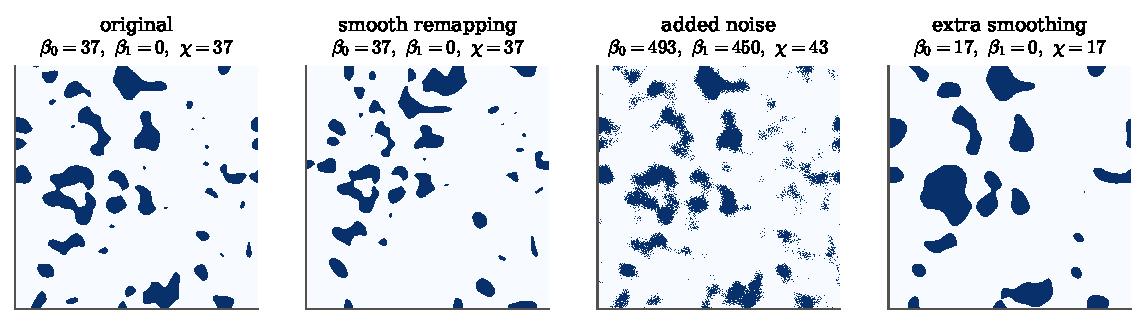
\includegraphics[width=\linewidth]{figures/ch12/nuisance_maps.pdf}
\caption{The pixels above one standard deviation (dark) for the original field and three of the transformed
ones. The smoothly remapped set looks distorted but has the same pieces and holes. Added noise covers the map
with tiny spurious pieces; extra smoothing merges or removes the small ones.}
\label{12a:fig:nuisance}
\end{figure}

\paragraph{Example: lensing of the microwave sky.} \Cref{T3a:sec:lensing} carried out this experiment with
real lensing deflections on flat patches of the simulated CMB sky. When the deflection was applied as a pure
remapping, the Euler characteristic (the pieces minus the holes, defined properly in
\cref{12a:sec:excursion}) changed only at the level of pixel ambiguities; when the beam was applied after the
lensing, the change grew to a few tenths of a per cent. That is the same pattern as the table above, with
the real nuisance in place of a toy one: the remapping is harmless, the smoothing that follows it is not.

\paragraph{Example: polarization singularities.} The polarization of the microwave background has points
where it vanishes and its direction is undefined, and around each the direction turns by a definite
half-integer number of turns, its index (\cref{T3a:sec:polarization}). A smooth one-to-one remapping can move
such a point and distort its surroundings, but it cannot change its index continuously, so the index is
protected \cite{VachaspatiLue2003,HutererVachaspati2005}. It fails exactly where the conditions fail: when two
singularities of opposite index annihilate, when one crosses the edge of the region, or when noise and
finite resolution blur it \cite{ChallinorChon2002}. The method of thought is the same in every example:
\emph{identify the nuisance first, then look for information it cannot easily erase}.

\subsection{Two different questions: what survives, and what changes}
\label{12a:sec:dynamics}

The invariance argument is easy to misuse. Topology is unchanged by smooth one-to-one deformations of a
\emph{region}. That does not mean the topology of a physical field is unchanged by the \emph{dynamics} that
evolves it. Gravitational collapse is not a remapping of the initial density: matter flows together, peaks
merge, filaments form and voids empty. The connectivity of the overdense regions at late times is genuinely
different from that at early times, and simulations of structure formation track exactly this change with
the counts of pieces, loops and voids and their persistence \cite{Pranav2017,Wilding2021}. There the change
\emph{is} the signal.

So topology answers two different questions, and an analysis must say which one it asks. For a nuisance
that acts like a smooth remapping, the question is \emph{what survives}, and the protected counts are the
answer. For a physical process that creates, destroys or reconnects structures, the question is \emph{what
changes because of the physics}, and the same counts are the record of it. In both cases the counts are
summaries of the data that the power spectrum does not expose: two fields can have identical spectra and
very different connectivity, like the rings and their phase-randomised twin of \cref{7a:sec:phases}. That
is the question behind the last row of the taxonomy of summaries in \cref{7a:sec:taxonomy}: is there
physically meaningful information in the way regions of the field are connected that the statistic we are
already using does not expose?
\section{The topology of a field: excursion sets and what we count in them}
\label{12a:sec:excursion}

A weather map shows the temperature over a country. Ask a forecaster for ``the topology of the temperature
field'' and the question has no answer: the country has a shape, and the field puts a number at every place
in it, but a list of numbers has no pieces or holes. Ask instead ``which regions are warmer than
$25^\circ$C?'' and the answer is a set of regions you can colour on the map. That coloured set has a
shape, and the shape can be counted: three warm regions, one of them with a cooler lake inside. This is the
whole trick. We do not assign a topology to the field; we use the field to cut out regions, and we count
the topology of the regions.

\subsection{Excursion sets}
\label{12a:sec:xnu}

Let the field be a map $\phi:\mathcal M\to\R$ from a domain $\mathcal M$ (a square patch, a periodic box,
the sky) to the real numbers. Throughout, $\phi$ is measured in units of its own standard deviation
$\sigma$, so a threshold $\nu=1$ means one standard deviation above the mean.

\begin{workdef}[excursion set, Betti numbers, Euler characteristic]
The \newterm{excursion set} at threshold $\nu$ is
\begin{equation}
  X_\nu=\{\bm x\in\mathcal M:\ \phi(\bm x)>\nu\},
  \label{12a:eq:xnu}
\end{equation}
the part of the domain where the field exceeds $\nu$ \unpack{on a CMB map, the directions hotter than the
threshold}. In two dimensions $\beta_0(X_\nu)$, the zeroth \newterm{Betti number}, is the number of
connected pieces of $X_\nu$ \unpack{pieces that cannot be joined by a path staying inside $X_\nu$}, and
$\beta_1(X_\nu)$ is the number of its holes \unpack{bounded regions of the complement, each fully enclosed by
$X_\nu$}. The \newterm{Euler characteristic} of a set in the plane is
\begin{equation}
  \chi(X_\nu)=\beta_0(X_\nu)-\beta_1(X_\nu) .
  \label{12a:eq:chi}
\end{equation}
\emph{Operationally:} colour the pixels above $\nu$, count the coloured pieces, count the uncoloured
regions that do not reach the edge, subtract.
\end{workdef}

Read \eqref{12a:eq:xnu} as a machine. The input is a field, which carries a number at every point; the
output is a set, which carries a shape. Everything in this chapter measures that set. For a CMB map
$T(\hat{\bm n})$ on the sphere, $X_\nu$ is literally the set of directions $\hat{\bm n}$ with
$T(\hat{\bm n})>\nu\sigma$, the hot spots at that threshold. ``Studying the topology of a field'' means
studying the topology of its excursion sets, threshold by threshold.

\emph{Why pieces minus holes?} Each Betti number on its own is a perfectly good count, and parts 12b
and 12c use them separately. The combination \eqref{12a:eq:chi} is singled out for two
reasons. First, it can be computed by purely local bookkeeping, counting corners, edges and squares, with no
need to find which pixels are connected to which (\cref{12a:sec:vef}). Second, its average over a Gaussian
random field can be calculated exactly (\cref{12a:sec:gkf}), which neither $\beta_0$ nor $\beta_1$ alone
allows. In three dimensions a solid region can also enclose sealed cavities, counted by $\beta_2$, and the
Euler characteristic becomes $\beta_0-\beta_1+\beta_2$ (\cref{T3a:sec:betti}).

\paragraph{Example: three shapes.} A disc has one piece and no hole: $\chi=1-0=1$. The ring of
\cref{12a:fig:deform} has one piece and one hole: $\chi=1-1=0$. A slice of Swiss cheese with three holes has
$\chi=1-3=-2$. Three separate discs have $\chi=3$. So $\chi$ is positive when the set is made of isolated
islands and negative when it is a connected sea full of lakes. A threshold scan will move between these
two extremes (\cref{12a:sec:scan}).

\emph{Why the counts survive deformations.} A continuous deformation that neither tears nor glues sends
paths to paths, so two points that could be joined inside the set can still be joined afterwards, and two
points that could not still cannot; the number of pieces is unchanged. A hole is a piece of the complement
fully surrounded by the set, and the same argument applied to the complement keeps the number of holes. In
fact more is true: the counts are unchanged even by continuous shrinkings, such as squeezing a ring down to a
thin circle, as long as nothing is cut (homotopy invariance; see the topology notes). That is why the
counts are robust to the smooth remapping of \cref{12a:sec:operator}, and why they are blind to how big or
how elongated the pieces are.

\subsection{Pixels: which pixels touch?}
\label{12a:sec:pixels}

A real map is a grid of pixels, and the excursion set is a set of coloured squares. To count pieces we
must decide when two coloured squares belong to the same piece. Two squares that share an edge clearly
touch. Two squares that meet only at a corner are the problem. Under the \newterm{4-neighbour} rule only
the four squares sharing an edge are neighbours; under the \newterm{8-neighbour} rule the four diagonal
squares are neighbours too.

\emph{Does the choice matter?} Look at the smallest troublesome pattern, a $2\times2$ block coloured like a
chessboard (\cref{12a:fig:pixels}, left). Under the 8-neighbour rule the two dark squares form one piece,
connected through their shared corner. If we also used the 8-neighbour rule for the light squares, they
too would form one piece, through the very same corner. Two paths, one dark and one light, would cross at a
point without either being interrupted. That cannot happen for regions in the plane: a closed curve
always separates its inside from its outside (the Jordan curve theorem; see the topology notes). So if the
dark set is 8-connected, its complement must be 4-connected, and vice versa. With this \newterm{dual}
convention every dark corner contact cuts the light squares apart there, and the counts of pieces and of
holes are consistent with each other.

There is a natural way to see which pairing we are using. Take each coloured pixel to be a \emph{closed}
unit square, edges and corners included. Two diagonal squares then share a corner point, so the union is
8-connected. The uncoloured part of the plane is what is left, the union of \emph{open} squares minus every
point that belongs to a coloured square; two uncoloured diagonal squares are separated by the coloured
corner between them, so the complement is 4-connected. Throughout this chapter the excursion set is the
union of closed squares of the pixels above threshold: 8-neighbours for the set, 4-neighbours for the
complement. The opposite choice, 4 for the set and 8 for the complement, is equally consistent; the two
choices give different counts only where the field crosses the threshold at a saddle inside a single
$2\times2$ block, which becomes rare when the field is smooth on the scale of a pixel (the last example of \cref{12a:sec:vef} measures how rare).

\begin{figure}[htbp]
\centering
\begin{tikzpicture}[scale=0.55]
  \begin{scope}[yshift=1.5cm]
    \fill[formblue!55] (0,1) rectangle (1,2);
    \fill[formblue!55] (1,0) rectangle (2,1);
    \draw[faint] (0,0) grid (2,2);
    \draw[very thick,formblue!80!black] (0.5,1.5) -- (1.5,0.5);
    \draw[very thick,fibreorange,dashed] (0.5,0.5) -- (1.5,1.5);
    \node[lbl,align=center,font=\footnotesize] at (1,-0.9) {8 for both:\\ paths cross};
  \end{scope}
  \foreach \thr/\xs/\ttl in {0.5/4.0/{$\nu=0.5$}, 1.5/10.0/{$\nu=1.5$}, 2.5/16.0/{$\nu=2.5$}}{
    \begin{scope}[xshift=\xs cm]
      \foreach \row/\vals in {0/{2,2,2,0,0}, 1/{2,0,2,0,1}, 2/{2,2,3,0,0}, 3/{0,0,0,1,0}, 4/{1,0,0,0,0}}{
        \foreach \v [count=\col from 0] in \vals {
          \pgfmathtruncatemacro{\inset}{\v>\thr ? 1 : 0}
          \ifnum\inset=1
            \fill[formblue!55] (\col,4-\row) rectangle ++(1,1);
          \fi
          \node[font=\scriptsize] at (\col+0.5,4.5-\row) {\v};
        }
      }
      \draw[faint] (0,0) grid (5,5);
      \node[lbl] at (2.5,-0.6) {\ttl};
    \end{scope}
  }
\end{tikzpicture}
\caption{Left: the chessboard pattern. If dark squares touching at a corner were connected and light ones
too, the dark path (solid) and the light path (dashed) would cross without either being broken; so the
complement of an 8-connected set must be 4-connected. Right: the $5\times5$ hand example. Each pixel shows its
field value; the pixels above the threshold are shaded.}
\label{12a:fig:pixels}
\end{figure}

\paragraph{Example: a $5\times5$ field by hand.} Take the field values of \cref{12a:fig:pixels}
(right), with row~1 at the top. At $\nu=0.5$ the coloured pixels are the seven 2s and the 3 that together
surround the central 0, and three 1s. Count the pieces with 8-neighbours. The ring of 2s and the 3 is
one piece. The 1 in row~4, column~4 touches the 3 at a corner, so it joins the ring. The 1 at the right end
of row~2 has no coloured neighbour at all, nor does the 1 at the bottom left. So $\beta_0=3$. Count the holes
with 4-neighbours for the uncoloured pixels: the central 0 of the ring is surrounded on all four sides and
cannot reach the edge, so it is a hole; every other uncoloured pixel reaches the edge. So $\beta_1=1$ and
$\chi=3-1=2$. With the opposite convention, the 1 that touched the 3 only at a corner is a separate piece,
$\beta_0=4$, while the hole remains, so $\chi=3$: the one diagonal contact is where the two conventions
disagree. At $\nu=1.5$ only the ring of 2s and the 3 survive: one piece with one hole, $\chi=0$ under both
conventions. At $\nu=2.5$ only the single 3 survives, $\chi=1$. The script
\pyname{code/ch12/02_grid_counting.py} repeats these counts in code and finds $\GridHandABzero$,
$\GridHandABone$, $\GridHandAChi$ (and $\GridHandAFourChi$ with the opposite convention) at $\nu=0.5$,
$\GridHandBChi$ at $1.5$ and $\GridHandCChi$ at $2.5$.

\paragraph{Counting pieces and holes in code.} Counting the pieces of a binary image is a standard task,
connected-component labelling, and \pyname{scipy.ndimage.label} does it for either neighbour rule. For the
holes we use the definition directly: a hole is a piece of the complement that does not reach the outside.
Surround the image with a one-pixel frame of uncoloured pixels, so that everything outside the image becomes
one single uncoloured piece; then label the uncoloured pixels with the dual rule and subtract that one
outside piece:
\pyfile[firstline=60,lastline=74]{code/ch12/lib_topo.py}{Betti numbers of a pixel set in the plane}
\noindent That a hole of a region in the plane is the same thing as a bounded piece of its complement is a
special property of the plane (and of the sphere), known as Alexander duality (see the topology notes). In
three dimensions holes are tunnels, and they cannot be found this way.

\subsection{The Euler characteristic as vertices minus edges plus faces}
\label{12a:sec:vef}

There is a second way to compute $\chi$ that never asks which pixels are connected. Think of the union of
closed squares as built from three kinds of cells: the lattice points at the corners of coloured pixels
(vertices, $V$ of them), the unit segments on the sides of coloured pixels (edges, $E$), and the coloured
pixels themselves (faces, $F$). Each vertex and each edge is counted once, however many coloured pixels
share it. Then
\begin{equation}
  \chi=V-E+F .
  \label{12a:eq:vef}
\end{equation}
This is the formula Euler found for polyhedra, and it holds for any set built of cells (see the topology
notes for the general statement). We can see why it agrees with $\beta_0-\beta_1$ for pixel sets by
building the set one pixel at a time and checking that both sides change by the same amount at every step.

\emph{One square on its own} has $V=4$, $E=4$, $F=1$: $\chi=4-4+1=1$, one piece and no hole.

\emph{Adding one more square.} Suppose the set is already built and we add one coloured square. The new
square brings one face. Some of its four vertices and four edges may already be present, namely those where
it touches the existing set. Call the part of its boundary where it touches the set the \emph{contact}. The
contact is made of $c$ separate arcs, each a path along the square's boundary made of $k_i$ edges and
$k_i+1$ vertices (an arc can be a single corner, $k_i=0$). Then
\begin{align}
  \Delta\chi
  &\eqby{1}\Delta V-\Delta E+1\nonumber\\
  &\eqby{2}\Big[4-\sum_{i=1}^{c}(k_i+1)\Big]-\Big[4-\sum_{i=1}^{c}k_i\Big]+1\nonumber\\
  &\eqby{3}1-c .
  \label{12a:eq:dchi}
\end{align}
\begin{explain}
  \item One new face; $\Delta V$ and $\Delta E$ are the vertices and edges of the new square that were not
        there before.
  \item The square has 4 vertices and 4 edges; the arcs of the contact already contain $k_i+1$ vertices and
        $k_i$ edges each.
  \item The 4s cancel and each arc contributes $-(k_i+1)+k_i=-1$.
\end{explain}
Now check $\beta_0-\beta_1$ in each case. If $c=0$ the square is isolated: a new piece, $\Delta\beta_0=+1$,
and \eqref{12a:eq:dchi} gives $+1$. If $c=1$ the square is glued to one piece along one arc, which changes
neither the number of pieces nor the number of holes, and \eqref{12a:eq:dchi} gives $0$. If $c=2$ the
square touches the set in two separate places. Either those two places belonged to different pieces, which
the square now joins ($\Delta\beta_0=-1$), or to the same piece, in which case the square closes a loop around
some uncoloured region and creates a hole ($\Delta\beta_1=+1$). Either way $\Delta(\beta_0-\beta_1)=-1=1-c$.
Each further arc merges one more piece or closes one more hole, and costs one more unit. The last case is a
square whose whole boundary is already present, a one-pixel hole being filled: then the contact is a closed
loop with 4 vertices and 4 edges, $\Delta V=\Delta E=0$, $\Delta\chi=+1$, and indeed one hole disappears,
$\Delta\beta_1=-1$. Since both sides start at $0$ for the empty set and change identically at every step,
$V-E+F=\beta_0-\beta_1$ for every pixel set.

\paragraph{Example: the ring by cells.} The $3\times3$ block of the hand example without its centre has the
$4\times4=16$ lattice points as vertices, $12$ horizontal and $12$ vertical unit edges (every side of the
central hole is also a side of a coloured neighbour), and $8$ faces: $\chi=16-24+8=0$, one piece and one hole,
as counted by hand.

The cell count is a sum of local terms, so it vectorises in a few lines of \pyname{numpy}. A lattice vertex is
present if any of the four pixels around it is coloured, an edge if either of the two pixels beside it is:
\pyfile[firstline=77,lastline=108]{code/ch12/lib_topo.py}{Euler characteristic as $V-E+F$ of the pixel complex}
\noindent The other branch builds the dual complex (4-neighbour convention), in which pixels are vertices,
edges join two coloured 4-neighbours and a face fills a fully coloured $2\times2$ block. The \texttt{periodic}
option treats the grid as a torus, which is how a field made with the fast Fourier transform really lives
(\cref{7a:sec:box}). On a torus a set could in principle wrap all the way around and have holes that are not
bounded lakes; at the thresholds and smoothing scales used here this never happens, and $\beta_1=\beta_0-\chi$.

\paragraph{Example: three methods on many fields.} The script \pyname{code/ch12/02_grid_counting.py} draws
$\GridNsim$ Gaussian fields on a $\GridN\times\GridN$ grid, smoothed on $\GridR$ pixels, and at each of $9$
thresholds between $-2$ and $2$ computes $\chi$ four ways: by labelling ($\beta_0-\beta_1$), by cells
($V-E+F$), by \pyname{skimage.measure.euler_number} with 8-connectivity, and by the Betti numbers that the
cubical-complex code of \pyname{gudhi} assigns to the same union of closed squares. In all $\GridNcase$ cases
the four answers agree exactly: $\GridMisBetti$, $\GridMisSk$ and $\GridMisGudhi$ mismatches. The cell count
takes $\GridTimeCells$\,ms per image, labelling $\GridTimeLabel$\,ms; \pyname{gudhi} takes
$\GridTimeGudhi$\,ms per field, but for that price it computes the counts at \emph{every} threshold at once,
which is what persistence will need in part~12b. \Cref{12a:fig:components} shows what is being counted on one
small map.

\begin{figure}[htbp]
\centering
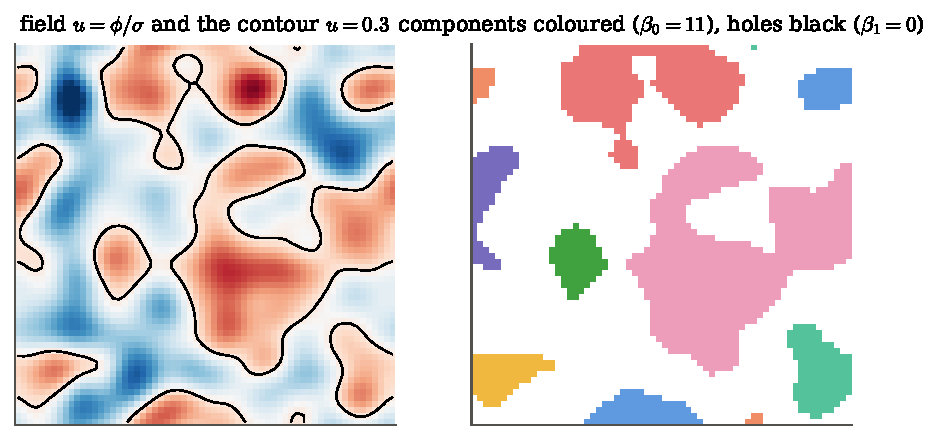
\includegraphics[width=0.9\linewidth]{figures/ch12/grid_components.pdf}
\caption{One $64\times64$ Gaussian field (left) with its contour at $\nu=0.3$, and the excursion set above
that contour (right). Each 8-connected piece has its own colour ($\beta_0=\GridFigBzero$); an uncoloured
region that cannot reach the edge is drawn black; this field has $\beta_1=\GridFigBone$ of them, so $\chi=\GridFigChi$.}
\label{12a:fig:components}
\end{figure}

\paragraph{Example: when does the convention matter?} The same script compares the two conventions on fields
smoothed on $R=1$, $2$, $4$ and $8$ pixels. The average difference $|\chi_8-\chi_4|$, as a fraction of the
average $|\chi_8|$, is $\GridConnDiffOne\%$, $\GridConnDiffTwo\%$, $\GridConnDiffFour\%$ and
$\GridConnDiffEight\%$. A field that changes from pixel to pixel produces many diagonal contacts and the
convention matters a great deal; a field smoothed over several pixels produces few, and the two conventions
converge. The practical rule: smooth the map on a scale of a few pixels or more before counting, and always
state the convention.

\begin{pitfall}[A count without a convention is not a measurement]
The same pixels give different Betti numbers under the 4- and the 8-neighbour rules, and an analysis that
uses 8-neighbours for both the set and its complement (or 4 for both) can report a hole count that is
inconsistent with its piece count. Fix the pairing (8 for the set, 4 for the complement, or the reverse),
use the same one for data and simulations, and smooth on several pixels so that the residual dependence is
small.
\end{pitfall}
\section{Scanning the threshold}
\label{12a:sec:scan}

Imagine flooding a hilly landscape. With the water level very low, only the deepest valleys are lakes and
the dry land is one continent full of holes. As the water rises the lakes grow and join, the continent breaks
into islands, and finally only a few mountain tops stick out. The dry land is the excursion set $X_\nu$ of
the height field, and the water level is the threshold $\nu$, lowered or raised. A single threshold catches
one moment of this story; scanning the threshold tells the whole of it.

\subsection{One map, all thresholds}
\label{12a:sec:onemap}

The script \pyname{code/ch12/03_threshold_scan.py} makes one Gaussian field on a $\ScanN\times\ScanN$ grid,
smoothed on $\ScanR$ pixels (the recipe of \cref{7a:sec:simulate}), scales it to zero mean and unit variance,
and computes $\beta_0$, $\beta_1$ and $\chi$ of the excursion set at thresholds from $-2.5$ to $2.5$ in steps
of $0.25$, with the functions of \cref{12a:sec:pixels}. Three rows of its output:
\begin{center}
\small
\begin{tabular}{rrrr}
\toprule
threshold $\nu$ & pieces $\beta_0$ & holes $\beta_1$ & $\chi=\beta_0-\beta_1$\\
\midrule
$-1$ & $\ScanMoneBzero$ & $\ScanMoneBone$ & $\ScanMoneChi$\\
$0$  & $\ScanZeroBzero$ & $\ScanZeroBone$ & $\ScanZeroChi$\\
$1$  & $\ScanOneBzero$  & $\ScanOneBone$  & $\ScanOneChi$\\
\bottomrule
\end{tabular}
\end{center}
At $\nu=-1$ about $84\%$ of the map is above threshold (a standard normal value exceeds $-1$ with probability
$0.84$). It forms one large connected sea with a few small islands beside it, and the cold spots
below $-1$ are its holes: $\chi$ is large and negative. At $\nu=0$ half the map is coloured and the set is a
tangle of large pieces and holes that nearly cancel. At $\nu=1$ only $16\%$ is coloured, in separate islands
around the hot spots, almost none of them with a hole: $\chi$ is large and positive. The full scan is
\cref{12a:fig:scan}. The number of pieces rises to a maximum of $\ScanBzeroMax$ near $\nu\approx1$ and then
falls, because at still higher thresholds the islands shrink and disappear one by one. The number of holes
does the mirror image at negative thresholds.

\begin{figure}[htbp]
\centering
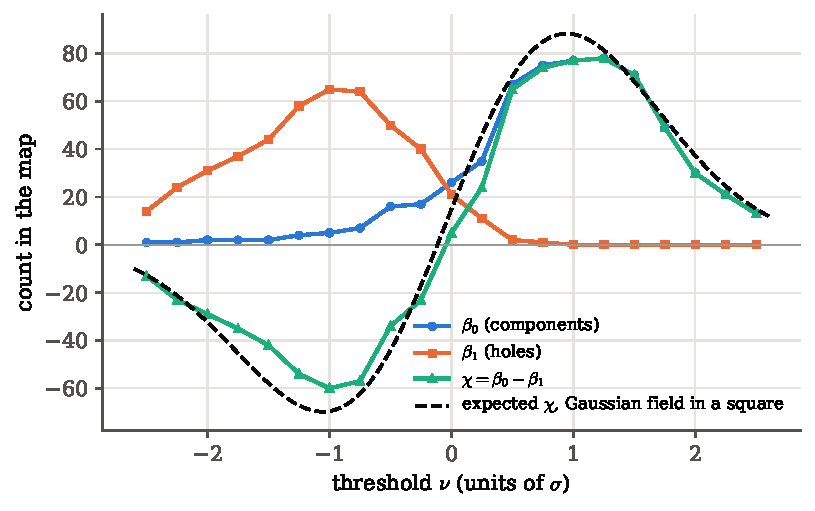
\includegraphics[width=0.75\linewidth]{figures/ch12/threshold_scan.pdf}
\caption{Pieces, holes and their difference for one $256\times256$ Gaussian map as the threshold is scanned.
Holes dominate at negative thresholds and pieces at positive ones; $\chi$ swings from negative to positive.
The dashed curve is the expected $\chi$ for a Gaussian field in a square, derived in
\cref{12a:sec:gkf,12a:sec:edges}.}
\label{12a:fig:scan}
\end{figure}

\paragraph{Example: the mirror symmetry.} The holes at $\nu=-1$ ($\ScanMoneBone$ of them) and the pieces at
$\nu=+1$ ($\ScanOneBzero$) are similar numbers. That is not a coincidence. A hole of $X_{-1}$ is a bounded
region where $\phi<-1$, which is a piece of the excursion set of the field $-\phi$ above $+1$. A Gaussian
field with zero mean is exactly as probable as its negative, so the cold spots of $\phi$ below $-1$ are
statistically identical to the hot spots of $\phi$ above $+1$. On average, then, $\beta_1(-\nu)$ equals
$\beta_0(+\nu)$ and $\chi(-\nu)=-\chi(\nu)$ (up to small corrections from the edges of the map, which
\cref{12a:sec:edges} computes). On one map the two counts differ by the realisation's own fluctuations. A
field whose hot spots and cold spots differ, for example one with a skewed distribution of values, breaks
this symmetry, and the asymmetry of the $\chi$ curve is one of the simplest tests of Gaussianity.

These numbers belong to one random map. They are not yet a measurement of anything: another map from the
same theory gives other numbers. They become a statistic only when we know how they scatter from map to
map, which is what the Monte Carlo of \cref{12a:sec:mc} and the whole of part~12c are about. The scan raises
a second question too: if one threshold is an arbitrary choice, why not keep track of every piece and every
hole as the threshold moves, recording at which level each appears and at which it disappears? That
bookkeeping is persistent homology, the subject of part~12b.

\subsection{A change of the values that changes nothing}
\label{12a:sec:monotone}

Suppose the field we observe is not $\phi$ but a pointwise, increasing function of it,
\begin{equation}
  \phi'(\bm x)=f\big(\phi(\bm x)\big),\qquad f'(\phi)>0 .
  \label{12a:eq:monotone}
\end{equation}
A change of units is such a function; so is the map from the initial density to a lognormal model of the
evolved density, $\phi'=e^{a\phi}$; so is the response of a detector that saturates smoothly. The function
changes every value but moves no point. \emph{What does it do to the excursion sets?} Move the threshold
along with the values:
\begin{align}
  \bm x\in X'_{f(\nu)}
  \;&\relby{1}{\Longleftrightarrow}\; f\big(\phi(\bm x)\big)>f(\nu)
  \;\relby{2}{\Longleftrightarrow}\; \phi(\bm x)>\nu
  \;\relby{3}{\Longleftrightarrow}\; \bm x\in X_\nu .
  \label{12a:eq:monotone-sets}
\end{align}
\begin{explain}
  \item The definition \eqref{12a:eq:xnu} of the excursion set of $\phi'$ at threshold $f(\nu)$.
  \item A strictly increasing function preserves order in both directions: $a>b$ if and only if
        $f(a)>f(b)$.
  \item The definition of the excursion set of $\phi$ at threshold $\nu$.
\end{explain}
So $X'_{f(\nu)}$ and $X_\nu$ are the same subset of the domain, point for point. Their pieces, holes, area and
boundary are identical. A monotone change of the values is a nuisance against which \emph{every} property of
the excursion sets is protected, provided the threshold is relabelled.

\emph{But we do not know $f$.} In practice nobody tells us the function; we only see $\phi'$. If we
threshold $\phi'$ in units of its own standard deviation, as we did for $\phi$, the thresholds no longer
correspond and the curves look different. There is one label that every monotone $f$ respects: the
\emph{fraction of the area} above threshold. By \eqref{12a:eq:monotone-sets} the set $X'_{f(\nu)}$ has the
same area as $X_\nu$. So instead of labelling a threshold by its value, label it by the area it encloses,
and convert that area back to a Gaussian-equivalent threshold $\nu_A$ through
\begin{equation}
  \Psi(\nu_A)=\text{fraction of the map above the threshold},\qquad
  \Psi(\nu)\equiv\int_\nu^\infty\frac{e^{-t^2/2}}{\sqrt{2\pi}}\,\dd t ,
  \label{12a:eq:nuA}
\end{equation}
the probability that a standard normal variable exceeds $\nu$. For a Gaussian field $\nu_A=\nu$ on average,
because the expected area fraction above $\nu$ is exactly $\Psi(\nu)$ (\cref{12a:sec:mfs}). For any monotone
function of a Gaussian field the excursion set at area-fraction threshold $\nu_A$ is the same set as the
Gaussian one at $\nu_A$. In code, the threshold with a given area fraction is a quantile of the map's values:
\pyfile[firstline=69,lastline=72]{code/ch12/03_threshold_scan.py}{The threshold that encloses a given area fraction}

\paragraph{Example: a lognormal field.} The same script takes $\MonoNsim$ Gaussian maps $\phi$ and their
lognormal versions $e^{0.8\phi}$, each standardised to zero mean and unit variance. Thresholded in units of
their own standard deviation (\cref{12a:fig:monotone}, left), the two $\chi$ curves disagree badly. At
$\nu=-1$ the Gaussian maps give a mean $\chi$ of $\MonoGaussMone$, the lognormal ones $\MonoLnRawMone$. The
reason is simple once found: the lognormal field is positive and skewed, so its standardised values cannot
go below about $-1.06$, and at $\nu=-1$ almost the whole map is above threshold, with very few holes.
Relabelled by area fraction (right panel), the two curves are identical; the script checks that the two
excursion sets coincide pixel for pixel at every threshold of every map: \MonoSame.

\paragraph{Example: a field that is not a monotone function of a Gaussian one.} Now take two independent
Gaussian fields $\phi$ and $\psi$ with the same spectrum and form $\phi^2+\psi^2$, a $\chi^2$ field with two
degrees of freedom, standardised. Its values are skewed like the lognormal's, but it is not a pointwise
function of a single Gaussian field: its value at a point depends on two independent fields, and its lowest
values sit only near the isolated points where both happen to vanish. Relabelling by area fraction cannot
undo that. At $\nu_A=1$ its
mean $\chi$ is $\MonoCtwoOne$ against the Gaussian $\MonoGaussOne$, and at $\nu_A=-1$ it is $\MonoCtwoMone$
against $\MonoGaussMone$. The remaining difference is information about how the field is arranged in space,
which no change of units can create or remove.

\begin{figure}[htbp]
\centering
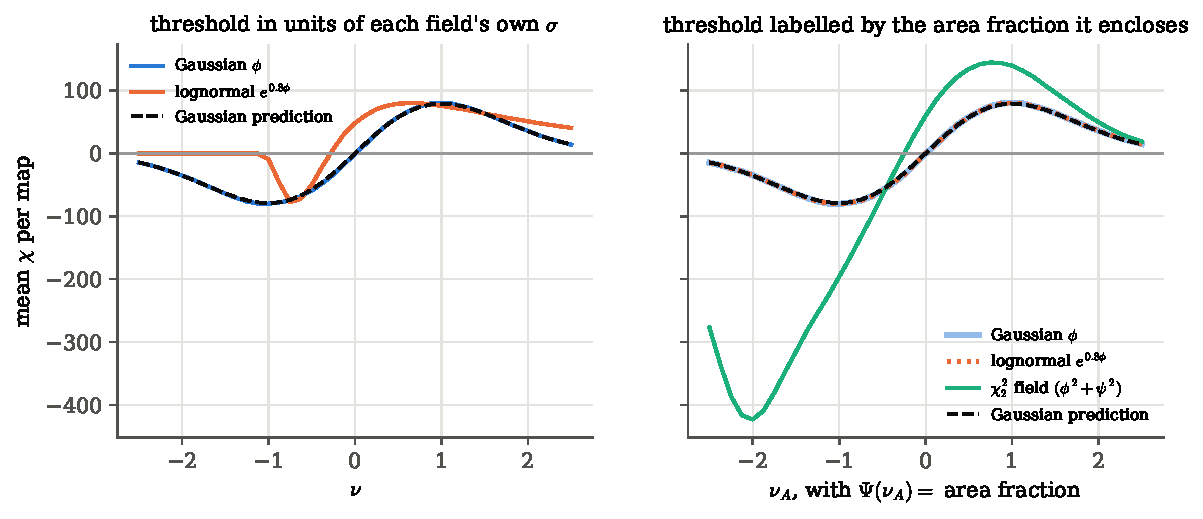
\includegraphics[width=\linewidth]{figures/ch12/monotone.pdf}
\caption{Mean $\chi$ per $256\times256$ map. Left: thresholds in units of each field's standard deviation;
the lognormal field (orange) looks very different from the Gaussian one (blue). Right: thresholds labelled by
the area fraction they enclose; the lognormal and Gaussian curves now lie exactly on top of each other, while
the $\chi^2$ field (green), which is not a monotone function of one Gaussian field, still differs.}
\label{12a:fig:monotone}
\end{figure}

\Cref{T3a:sec:relabel} reached the same conclusion from the other side, for the slightly skewed skies of
weakly non-Gaussian models: the part of the change in the Minkowski functionals that comes from a pointwise
distortion of the values is only a sideways shift of the curves, and it disappears at fixed area fraction.
What the two examples here add is the exact, non-perturbative version: for \emph{any} increasing function,
however strongly non-Gaussian the values, the curves at fixed area fraction are untouched. Two lessons
follow. First, labelling by area fraction separates the information carried by the one-point distribution of
values (which a histogram of the map already gives) from the information about spatial arrangement, which is
what topology is for. Second, the same argument marks the limit of the invariance discussed in
\cref{12a:sec:dynamics}: gravitational evolution is not a pointwise function of the initial density, because
it moves matter, so its effect on the excursion sets does not disappear under relabelling. That is why the
topology of the evolved density field carries information about the dynamics.
\section{Area, boundary length and Euler characteristic}
\label{12a:sec:mfs}

The microwave-sky chapter already measured the shapes of hot spots with three numbers
(\cref{T3a:sec:morphology}): the area fraction of the excursion set, a quarter of its boundary length per
steradian, and its Euler characteristic per steradian, called $v_0$, $v_1$ and $v_2$. There we derived the
expected area fraction and boundary length of a Gaussian sky, \eqref{T3a:eq:v0} and \eqref{T3a:eq:v1}, and
stated the expected Euler characteristic \eqref{T3a:eq:v2} without proof, promising the derivation for this
chapter. Two things are different now. The field lives on a flat square grid, so lengths are in pixels and
there is no curvature of the domain to worry about until \cref{12a:sec:sphere}. And we need the Euler
characteristic not as a number to be quoted but as a quantity we can compute, which means writing it in a
form that the counting argument of \cref{12a:sec:gkf} can attack.

\subsection{Three numbers per threshold}
\label{12a:sec:three}

Why exactly these three? Suppose we want a number $S(X)$ that describes the shape of a region $X$ of the
plane and has three properties. It is \emph{additive}: for two regions,
$S(X\cup Y)=S(X)+S(Y)-S(X\cap Y)$, so the shape number of a set of separate islands is the sum over the
islands. It is \emph{motion invariant}: moving or rotating the region does not change it, which is what we
want on a statistically homogeneous and isotropic sky. And it changes \emph{continuously} when the region is
changed a little. Hadwiger's theorem says that every such $S$ is a linear combination of three numbers: the
area $A$, the boundary length $L$, and the Euler characteristic $\chi$ \cite{SchmalzingGorski1998}. In this
sense the three are a complete set of shape measures of this kind; any other such measure contains no new
information. They are the \newterm{Minkowski functionals} of the region.

\begin{workdef}[Minkowski functionals of an excursion set]
For a field $u=\phi/\sigma$ on a region of area $A_{\rm tot}$, and a threshold $\nu$:
\begin{itemize}[itemsep=1pt,leftmargin=1.2em]
  \item area fraction $a(\nu)=\mathrm{area}(X_\nu)/A_{\rm tot}$ \unpack{the share of pixels above $\nu$};
  \item boundary length per unit area $\ell(\nu)=\mathrm{length}(\partial X_\nu)/A_{\rm tot}$ \unpack{the
        total length of the contour $u=\nu$ per unit area};
  \item Euler characteristic per unit area $c(\nu)=\chi(X_\nu)/A_{\rm tot}$ \unpack{pieces minus holes per
        unit area}.
\end{itemize}
On the sky, $v_0=a$, $v_1=\ell/4$ and $v_2=c$ (with the sphere's own curvature removed, \cref{12a:sec:sphere}).
\end{workdef}

The area fraction and the boundary length are the ``metric'' functionals: a smooth remapping changes them
(\cref{12a:sec:operator}). The Euler characteristic is the topological one. Yet Hadwiger's theorem puts it on
the same footing, as the third member of a family. To see how a count of pieces can be a functional of the
same kind as a length, we need one more way of writing it.

\subsection{The Euler characteristic as the total turning of the boundary}
\label{12a:sec:turning}

Walk once around the boundary of a disc, keeping the disc on your left. Your direction of travel turns
steadily, and by the time you are back at the start it has turned through one full circle, $2\pi$. Now walk
around a lake inside an island, again keeping the land on your left: you go around the lake clockwise, and
your direction turns through $-2\pi$. Deform the island and the lake however you like: the walk can wiggle,
turning left and right, but every left turn that is not undone by a right turn would leave you facing a new
direction at the end, and you must end facing the way you started, having gone once around. So the total
turning of a closed boundary curve without self-crossings is exactly $\pm2\pi$, whatever its shape (the
turning-tangent theorem; see the topology notes).

The rate of turning per unit length is the \newterm{curvature} of the boundary, $\kappa$: on a circle of
radius $r$ it is $1/r$, so the total turning is $\kappa\times$length $=(1/r)(2\pi r)=2\pi$. Add up the total
turning over all the boundary curves of a region, each walked with the region on the left. Each piece has
one outer boundary and contributes $+2\pi$; each hole has one boundary walked clockwise and contributes
$-2\pi$. Therefore
\begin{equation}
  \frac{1}{2\pi}\oint_{\partial X}\kappa\,\dd l=\beta_0(X)-\beta_1(X)=\chi(X) .
  \label{12a:eq:chi-curv}
\end{equation}
This is the bridge. The Euler characteristic is the integral, along the boundary, of a local geometric
quantity, the curvature, exactly as the boundary length is the integral of $1$ along the boundary. That is
why it belongs with the area and the length, and why it is the quantity $V_2$ of
\cite{SchmalzingGorski1998} (their eq.~6, $V_2=\frac{1}{2\pi}\int\kappa\,\dd l$).

\begin{figure}[htbp]
\centering
\begin{tikzpicture}[scale=1.0]
  \fill[formblue!25,even odd rule]
    plot[smooth cycle,tension=0.75] coordinates {(-2.2,0) (-1.4,1.3) (0.2,1.0) (1.6,1.5) (2.4,0.2) (1.2,-1.2) (-0.6,-0.9) (-1.8,-1.1)}
    (0.3,0.05) ellipse (0.75 and 0.45);
  \draw[form,midarrow=0.3]
    plot[smooth cycle,tension=0.75] coordinates {(-2.2,0) (-1.4,1.3) (0.2,1.0) (1.6,1.5) (2.4,0.2) (1.2,-1.2) (-0.6,-0.9) (-1.8,-1.1)};
  \draw[bdry,postaction={decorate},decoration={markings,mark=at position 0.3 with {\arrow{Stealth[length=2.2mm,reversed]}},
        mark=at position 0.8 with {\arrow{Stealth[length=2.2mm,reversed]}}}] (0.3,0.05) ellipse (0.75 and 0.45);
  \draw[vec] (-2.2,0) -- ++(0,-0.7);
  \draw[vec] (1.6,1.5) -- ++(-0.75,0.05);
  \draw[vec] (2.4,0.2) -- ++(0.0,0.75);
  \node[lbl,anchor=west] at (2.7,0.0) {outer boundary: $+2\pi$};
  \node[lbl,bdryred,anchor=north] at (0.3,-0.55) {lake: $-2\pi$};
  \fill[formblue!25] (4.6,1.2) circle (0.45);
  \draw[form,midarrow=0.3] (4.6,1.2) circle (0.45);
  \node[lbl,anchor=west] at (5.15,1.2) {island: $+2\pi$};
\end{tikzpicture}
\caption{Walking each boundary with the set (blue) on the left. The outer boundary of a piece turns in total
by $+2\pi$, however wiggly it is; the shore of a lake is walked clockwise and turns by $-2\pi$. The total
turning divided by $2\pi$ is pieces minus holes, here $2-1=1$. The green arrows show the direction of travel
at three places.}
\label{12a:fig:turning}
\end{figure}

\paragraph{Example: a disc and a ring.} A disc of radius $r$: curvature $1/r$ along a length $2\pi r$, so
\eqref{12a:eq:chi-curv} gives $\frac{1}{2\pi}\cdot2\pi=1$. A ring with radii $r_1<r_2$: the outer circle
gives $+1$, the inner circle, walked clockwise, has curvature $-1/r_1$ along $2\pi r_1$ and gives $-1$; total
$0$. Neither result depends on the radii, as it must not.

\paragraph{Example: a cap on the sphere.} On a curved surface the walk also turns because the surface itself
curves, and \eqref{12a:eq:chi-curv} acquires a term from the area. Take the polar cap of angular radius
$\theta$ on the unit sphere, the set of points within angle $\theta$ of the north pole. Its boundary is a
circle of latitude of length $2\pi\sin\theta$, whose curvature measured within the sphere (the geodesic
curvature) is $\cot\theta$. The surface has Gaussian curvature $K=1$, and the cap has area
$2\pi(1-\cos\theta)$. The Gauss--Bonnet theorem (see the topology notes) adds the integrated surface curvature
to the turning of the boundary:
\begin{align}
  \chi(\text{cap})
  &\eqby{1}\frac{1}{2\pi}\Big[\oint\kappa_g\,\dd l+\int_{\rm cap}K\,\dd A\Big]\nonumber\\
  &\eqby{2}\frac{1}{2\pi}\Big[\cot\theta\cdot2\pi\sin\theta+2\pi(1-\cos\theta)\Big]\nonumber\\
  &\eqby{3}\cos\theta+1-\cos\theta=1 .
  \label{12a:eq:cap}
\end{align}
\begin{explain}
  \item Gauss--Bonnet for a region of a curved surface: boundary turning plus enclosed curvature, over
        $2\pi$.
  \item Geodesic curvature $\cot\theta$ times the length $2\pi\sin\theta$ of the circle; $K=1$ times the area
        of the cap.
  \item $\cot\theta\sin\theta=\cos\theta$.
\end{explain}
The cap is one piece without holes at every size, and the two terms trade off exactly as $\theta$ grows. When
$\theta\to\pi$ the boundary shrinks to a point near the south pole and the area term alone gives
$\frac{1}{2\pi}\cdot4\pi=2$, the Euler characteristic of the whole sphere. This is the origin of the extra
term in the full-sky formula of \cite{SchmalzingGorski1998} (their eq.~7), $\chi=V_2+V_0/(2\pi R^2)$ on a
sphere of radius $R$, which \cref{12a:sec:sphere} needs.

\subsection{Area and length of a Gaussian field, recalled in the plane}
\label{12a:sec:area-length}

Let $u=\phi/\sigma$ be a statistically homogeneous and isotropic Gaussian field with zero mean and unit
variance in the plane. The quantity that sets the scale of everything below is the variance of one
component of its gradient,
\begin{equation}
  \lambda\equiv\big\langle(\partial_xu)^2\big\rangle=\tfrac12\big\langle|\nabla u|^2\big\rangle
  =\frac{\sigma_1^2}{2\sigma_0^2},
  \label{12a:eq:lambda}
\end{equation}
where $\sigma_0^2$ is the variance of $\phi$ and $\sigma_1^2=\langle|\nabla\phi|^2\rangle$ the variance of its
gradient, the spectral moments of \eqref{7a:eq:moments}. The two components contribute equally by isotropy,
hence the $\frac12$. On the sky, \eqref{T3a:eq:thetac} defined the correlation angle $\theta_c=\sigma_0/\sigma_1$,
so $\lambda=1/(2\theta_c^2)$. A large $\lambda$ means a field that changes quickly, with many small spots.

\emph{The area.} The expected fraction of the plane above $\nu$ is the probability that the field at one
point exceeds $\nu$ (the plane average equals the ensemble average at a point, by homogeneity and ergodicity,
\cref{7a:sec:ergodic}):
\begin{equation}
  \E[a(\nu)]=\Prob(u>\nu)=\Psi(\nu) ,
  \label{12a:eq:area}
\end{equation}
with $\Psi$ the Gaussian tail of \eqref{12a:eq:nuA}.

\emph{The length.} Thicken the contour $u=\nu$ into the thin band $\nu<u<\nu+\dd\nu$. Where the gradient is
$|\nabla u|$, the band has width $\dd\nu/|\nabla u|$, so its area is the contour length times
$\dd\nu/|\nabla u|$, averaged along the contour. Turned around, the length per unit area is the area fraction
of the band, weighted by $|\nabla u|$ and divided by $\dd\nu$, which is the expectation of
$|\nabla u|\,\delta(u-\nu)$:
\begin{align}
  \E[\ell(\nu)]
  &\eqby{1}\E\big[|\nabla u|\,\delta(u-\nu)\big]
   \eqby{2}\frac{e^{-\nu^2/2}}{\sqrt{2\pi}}\,\E|\nabla u|
   \eqby{3}\frac{e^{-\nu^2/2}}{\sqrt{2\pi}}\sqrt{\frac{\pi\lambda}{2}}
   \eqby{4}\frac{\sqrt\lambda}{2}\,e^{-\nu^2/2} .
  \label{12a:eq:length}
\end{align}
\begin{explain}
  \item The band argument above (the coarea formula).
  \item At one point $u$ and $\nabla u$ are uncorrelated, $\langle u\,\partial_iu\rangle=\frac12\partial_i\langle
        u^2\rangle=0$ for a homogeneous field, and uncorrelated jointly Gaussian variables are independent; the
        average of $\delta(u-\nu)$ is the standard normal density at $\nu$.
  \item $|\nabla u|$ is the length of a two-component vector with independent $\Normal(0,\lambda)$ components,
        a Rayleigh variable with mean $\sqrt{\lambda}\sqrt{\pi/2}$ (\cref{T3a:sec:mf-gauss}).
  \item $\frac{1}{\sqrt{2\pi}}\sqrt{\frac{\pi}{2}}=\frac12$.
\end{explain}
On the sky \eqref{T3a:eq:v1} is the same result with $v_1=\ell/4$ and $\lambda=1/(2\theta_c^2)$:
$\frac14\cdot\frac{1}{2\sqrt2\,\theta_c}=\frac{1}{8\sqrt2\,\theta_c}$. The Euler characteristic is the one
functional that needs the second derivatives of the field, because curvature is a second derivative. Its
derivation is the next section.

\paragraph{Example: the numbers on simulated maps.} The library function \pyname{mfs_flat}
measures all three on a periodic map: the area fraction by counting pixels, the
length from \eqref{12a:eq:length} with the delta function replaced by a narrow top hat of width $0.1$ and the
gradient computed exactly by the fast Fourier transform, and $\chi$ by $V-E+F$. Over $\GkfNsim$ maps of
$\GkfN\times\GkfN$ pixels with $\lambda=\GkfLamNZero$ per pixel$^2$ (\cref{12a:sec:mc}), the mean area fraction
at $\nu=1$ is $\GkfAreaOneMC$ against $\Psi(1)=\GkfAreaOneTh$, and the mean length per unit area at $\nu=0$ is
$\GkfLenZeroMC$ against $\GkfLenZeroTh$ per pixel from \eqref{12a:eq:length}, a difference of
$\GkfLenZeroRel\%$ (\cref{12a:fig:gkf-plane}).

\begin{figure}[htbp]
\centering
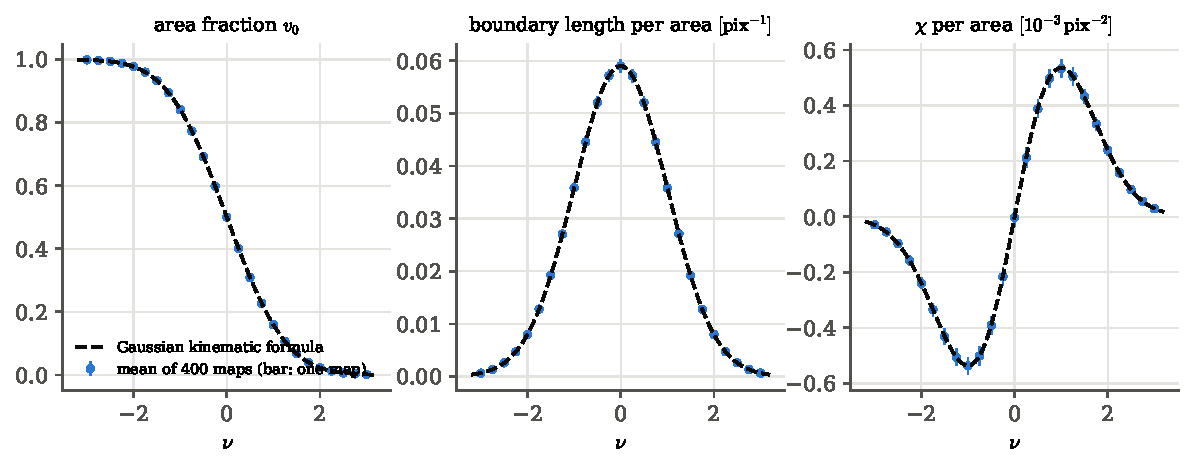
\includegraphics[width=\linewidth]{figures/ch12/gkf_plane.pdf}
\caption{The three Minkowski functionals of the excursion sets of $\GkfNsim$ Gaussian maps
($\GkfN\times\GkfN$ pixels, white noise smoothed on $6$ pixels). Points: the mean over the maps; bars: the
scatter of a single map. Dashed: the Gaussian predictions \eqref{12a:eq:area}, \eqref{12a:eq:length} and,
for $\chi$, \eqref{12a:eq:gkf2}.}
\label{12a:fig:gkf-plane}
\end{figure}

\section{The expected Euler characteristic of a Gaussian field}
\label{12a:sec:gkf}

Counting pieces needs the whole map: to know whether two hot pixels at opposite ends of a long filament
belong to one piece we must follow the filament. An average over random fields of such a global count looks
hopeless. Yet for a Gaussian field the average Euler characteristic at every threshold has a short closed
formula. The trick that makes it possible is to trade the global count for a sum of local events, each of
which happens at a single point, and then to ask how often such points occur. That is a question about
derivatives of the field at one point, and for a Gaussian field the joint distribution of the value and the
derivatives at one point is known exactly. Once the formula is in hand, it tells us what $\chi(\nu)$ can and
cannot know about the power spectrum.

\paragraph{The question.} For a homogeneous, isotropic Gaussian field $u$ with zero mean and unit variance,
what is the expected Euler characteristic of $X_\nu=\{u>\nu\}$ per unit area?

\subsection{From a global count to local events}
\label{12a:sec:morse}

Go back to the flooding picture of \cref{12a:sec:scan}, and lower the water level $\nu$ from far above the
highest peak. The dry land $X_\nu$ changes its pieces and holes only at particular levels, and each change
happens at one point. Which points? A point where the land is sloped is boring: lowering the water a little
just moves the shore there. Something can happen only where the ground is flat, at a \newterm{critical point}
of the height, where the gradient vanishes. In two dimensions there are three kinds, told apart by the
second derivatives (the Hessian matrix $H_{ij}=\partial_i\partial_ju$):
\begin{itemize}[itemsep=1pt,leftmargin=1.2em]
  \item \emph{A peak} (both eigenvalues of $H$ negative). When the water drops below it, a new island appears:
        $\beta_0$ goes up by one, so $\chi$ goes up by one.
  \item \emph{A saddle} (one eigenvalue of each sign), a mountain pass. When the water drops below it, the
        land on its two sides joins through the pass. Either the two sides were different islands, which merge
        ($\beta_0$ down by one), or they were already connected the long way round, and the new connection
        closes a ring around a lake ($\beta_1$ up by one). Either way $\chi$ goes down by one.
  \item \emph{A pit} (both eigenvalues positive), the bottom of a lake. When the water drops below it, the lake
        dries up: $\beta_1$ goes down by one and $\chi$ goes up by one.
\end{itemize}
Starting from the empty set ($\chi=0$) at very high water and adding up the changes,
\begin{equation}
  \chi(X_\nu)=\#\{\text{peaks above }\nu\}-\#\{\text{saddles above }\nu\}+\#\{\text{pits above }\nu\},
  \label{12a:eq:morse}
\end{equation}
for a field on a domain without edges (a periodic box; edges are added in \cref{12a:sec:edges}). This is the
counting rule of Morse theory, and it is the second definition of the Euler characteristic quoted by
\cite{HamiltonGottWeinberg1986} (their eq.~7). Its sign pattern can be written with the Hessian alone: the
determinant $\det H$ is positive at peaks and pits (two eigenvalues of the same sign) and negative at
saddles. So
\begin{equation}
  \chi(X_\nu)=\sum_{\text{critical points }\bm x_c\text{ with }u(\bm x_c)>\nu}\operatorname{sign}\det H(\bm x_c).
  \label{12a:eq:morse-sign}
\end{equation}

\begin{figure}[htbp]
\centering
\begin{tikzpicture}
\begin{axis}[width=8.6cm,height=4.4cm,xmin=0.3,xmax=9.2,ymin=-1.7,ymax=1.9,axis lines=left,
  xlabel={$x$},ylabel={$u(x)$},xtick=\empty,ytick={0.3},yticklabels={$\nu$},
  label style={font=\small},tick label style={font=\small}]
  \addplot[form,domain=0.3:9.2,samples=200,name path=f] {1.2*sin(deg(0.9*x))+0.6*sin(deg(2.5*x+0.5))};
  \addplot[bdryred,thick,domain=0.3:9.2,name path=lev] {0.3};
  \addplot[formblue!25] fill between[of=f and lev,soft clip={domain=0.3:3.42}];
  \addplot[formblue!25] fill between[of=f and lev,soft clip={domain=7.31:9.2}];
  \addplot[only marks,mark=*,mark size=1.8pt] coordinates {(0.68,1.17) (2.71,1.28) (8.12,1.58)};
  \addplot[only marks,mark=o,mark size=1.8pt] coordinates {(1.66,0.60)};
\end{axis}
\end{tikzpicture}
\hspace{0.4cm}
\begin{tikzpicture}[scale=0.85]
  \begin{scope}
    \foreach \r in {0.3,0.6,0.9} \draw[form] (0,0) circle (\r);
    \fill (0,0) circle (1.6pt);
    \node[lbl] at (0,-1.3) {peak: $+1$};
  \end{scope}
  \begin{scope}[xshift=2.6cm]
    \clip (-1.1,-1.1) rectangle (1.1,1.1);
    \foreach \c in {0.15,0.45,0.8} {
      \draw[form,domain=-1:1,samples=40] plot ({\x},{sqrt(\x*\x+\c)});
      \draw[form,domain=-1:1,samples=40] plot ({\x},{-sqrt(\x*\x+\c)});
      \draw[faint,domain=-1:1,samples=40] plot ({sqrt(\x*\x+\c)},{\x});
      \draw[faint,domain=-1:1,samples=40] plot ({-sqrt(\x*\x+\c)},{\x});
    }
    \fill (0,0) circle (1.6pt);
  \end{scope}
  \node[lbl] at (2.6,-1.3) {saddle: $-1$};
  \begin{scope}[xshift=5.2cm]
    \foreach \r in {0.3,0.6,0.9} \draw[faint] (0,0) circle (\r);
    \fill (0,0) circle (1.6pt);
    \node[lbl] at (0,-1.3) {pit: $+1$};
  \end{scope}
\end{tikzpicture}
\caption{Left: in one dimension the excursion set above $\nu$ (red line) is a union of intervals (shaded).
Each interval contains one more peak (filled dots) than pits (open dot) above the level: two peaks and one
pit in the first, one peak in the second. Right: the three kinds of critical point in
two dimensions, drawn as contour lines (blue rising towards the centre, grey falling). Lowering the threshold
past each changes $\chi$ by the amount shown.}
\label{12a:fig:critical}
\end{figure}

\subsection{The simplest case first: a line}
\label{12a:sec:rice}

On a line the excursion set is a union of intervals, and its Euler characteristic is the number of
intervals. Lowering the level, a new interval appears at a peak and two intervals merge at a pit, so the
counting rule reads $\chi=\#\{\text{peaks above }\nu\}-\#\{\text{pits above }\nu\}$ (\cref{12a:fig:critical},
left). On a long line each interval begins where the field crosses $\nu$ going up, so the number of
intervals per unit length is also the rate of \emph{up-crossings} of the level. We compute it both ways; the
agreement is the first check of the method.

\emph{The ingredients.} At one point $x$ we need the joint distribution of the value $u$, the slope $u'$ and
the curvature $u''$. They are jointly Gaussian with zero mean (derivatives of a Gaussian field are linear
combinations of its values, so they are Gaussian too). Write $\lambda=\langle u'^2\rangle$, the
one-dimensional version of \eqref{12a:eq:lambda}. Every covariance we need follows from one identity. For a
homogeneous field the average of any product of the field and its derivatives is the same at every point, so
its derivative vanishes: $\frac{\dd}{\dd x}\langle fg\rangle=0$, hence
\begin{equation}
  \langle f'g\rangle=-\langle fg'\rangle\qquad\text{(moving a derivative costs a sign)}.
  \label{12a:eq:move}
\end{equation}
With $f=g=u$ it gives $\langle u'u\rangle=-\langle uu'\rangle$, so $\langle uu'\rangle=0$. With $f=u'$, $g=u'$
it gives $\langle u''u'\rangle=0$. With $f=u'$, $g=u$ it gives $\langle u''u\rangle=-\langle u'u'\rangle=-\lambda$.
So the slope is uncorrelated with both the value and the curvature, and being jointly Gaussian it is
independent of them; the value and the curvature are correlated, with covariance $-\lambda$.

\emph{How many up-crossings in a short step $\dd x$?} An up-crossing happens between $x$ and $x+\dd x$ if the
field starts below the level and ends above it, $u<\nu<u+u'\dd x$, which needs $u'>0$ and
$\nu-u'\dd x<u<\nu$. The probability of that is
\begin{align}
  \Prob(\text{up-crossing in }\dd x)
  &\eqby{1}\int_0^\infty\dd u'\int_{\nu-u'\dd x}^{\nu}p(u,u')\,\dd u
   \eqby{2}\dd x\int_0^\infty u'\,p(\nu,u')\,\dd u'\nonumber\\
  &\eqby{3}\dd x\;\frac{e^{-\nu^2/2}}{\sqrt{2\pi}}\int_0^\infty u'\,\frac{e^{-u'^2/2\lambda}}{\sqrt{2\pi\lambda}}\,\dd u'
   \eqby{4}\dd x\;\frac{e^{-\nu^2/2}}{\sqrt{2\pi}}\,\sqrt{\frac{\lambda}{2\pi}}
   =\dd x\;\frac{\sqrt\lambda}{2\pi}\,e^{-\nu^2/2}.
  \label{12a:eq:rice}
\end{align}
\begin{explain}
  \item Integrate the joint density of value and slope over the region just described.
  \item The inner range has length $u'\dd x$, so for small $\dd x$ the inner integral is the integrand at
        $u=\nu$ times $u'\dd x$.
  \item The value and the slope are independent, so the joint density factorises into two Gaussians, of
        variance $1$ and $\lambda$.
  \item $\int_0^\infty s\,e^{-s^2/2\lambda}\dd s=\lambda$, divided by $\sqrt{2\pi\lambda}$.
\end{explain}
This is Rice's formula for the rate of level crossings \cite{Rice1944}: the expected number of intervals of
$\{u>\nu\}$ per unit length is $\frac{\sqrt\lambda}{2\pi}e^{-\nu^2/2}$.

\emph{The same number by counting critical points.} Now use the counting rule instead. A critical point is a
zero of the slope $u'$. Near a zero $x_c$ the slope is $u'(x)\approx u''(x_c)(x-x_c)$, so the delta function
$\delta(u'(x))$ integrated over a small neighbourhood gives $1/|u''(x_c)|$; multiplied by $|u''|$ it counts
the zero exactly once. Peaks have $u''<0$ and pits $u''>0$, so $\delta(u')\,(-u'')$ counts peaks as $+1$ and
pits as $-1$, which is exactly the sign rule. Averaging:
\begin{align}
  \frac{\E[\chi]}{\text{length}}
  &\eqby{1}\E\big[\delta(u')\,(-u'')\,\mathbb 1\{u>\nu\}\big]
   \eqby{2}p_{u'}(0)\;\E\big[(-u'')\,\mathbb 1\{u>\nu\}\big]\nonumber\\
  &\eqby{3}\frac{1}{\sqrt{2\pi\lambda}}\int_\nu^\infty\lambda u\,\frac{e^{-u^2/2}}{\sqrt{2\pi}}\,\dd u
   \eqby{4}\frac{\lambda}{\sqrt{2\pi\lambda}}\,\frac{e^{-\nu^2/2}}{\sqrt{2\pi}}
   =\frac{\sqrt\lambda}{2\pi}\,e^{-\nu^2/2}.
  \label{12a:eq:kr1}
\end{align}
\begin{explain}
  \item The counting rule, with each critical point counted by $\delta(u')|u''|$ and signed by
        $-\operatorname{sign}u''$; the indicator $\mathbb 1\{u>\nu\}$ keeps only critical points above the
        level. On a homogeneous line the average per unit length is the average at one point.
  \item The slope is independent of the value and the curvature, so the average splits; the average of
        $\delta(u')$ is the density of $u'$ at zero.
  \item The density of $u'$ at zero is $1/\sqrt{2\pi\lambda}$. For the curvature we only need its average at a
        given value $u$. For jointly Gaussian variables with zero mean the conditional mean is linear,
        $\E[Y\given X]=\frac{\Cov(X,Y)}{\Var X}X$ (\cref{ch:02}); with $\Cov(u,u'')=-\lambda$ and $\Var u=1$,
        $\E[-u''\given u]=\lambda u$.
  \item $\int_\nu^\infty u\,e^{-u^2/2}\dd u=e^{-\nu^2/2}$.
\end{explain}
The two routes agree. The second one is the one that generalises, because it never needed to know what an
interval is, only how to recognise and sign a critical point.

\subsection{The plane}
\label{12a:sec:gkf2}

\emph{Counting critical points in two dimensions.} The critical points are the zeros of the gradient
$\nabla u$, a map from the plane to the plane. Near a zero, $\nabla u(\bm x)\approx H(\bm x_c)(\bm x-\bm x_c)$,
and the two-dimensional delta function $\delta^2(\nabla u)$ integrated over a neighbourhood gives
$1/|\det H|$, the inverse Jacobian of that linear map. So $\delta^2(\nabla u)\,|\det H|$ counts each critical
point once, and $\delta^2(\nabla u)\det H$ counts it with the sign of \eqref{12a:eq:morse-sign}. Averaging
over the field, per unit area,
\begin{equation}
  \E[c(\nu)]=\E\big[\delta^2(\nabla u)\,\det H\;\mathbb 1\{u>\nu\}\big].
  \label{12a:eq:kr2}
\end{equation}
This is the two-dimensional version of the first line of \eqref{12a:eq:kr1}, the Kac--Rice counting
formula. The absolute value that would make the average of $|\det H|$ hard has disappeared, because the sign
rule wants $\det H$ itself, a polynomial in the second derivatives.

\emph{The ingredients.} The identity \eqref{12a:eq:move} holds for derivatives in any direction. It gives,
exactly as on the line:
\begin{itemize}[itemsep=1pt,leftmargin=1.2em]
  \item $\langle u\,\partial_iu\rangle=0$ and $\langle\partial_iu\,\partial_j\partial_ku\rangle=0$: the
        gradient is independent of the value and of the Hessian at the same point.
  \item $\langle u\,\partial_i\partial_ju\rangle=-\langle\partial_iu\,\partial_ju\rangle=-\lambda\delta_{ij}$:
        by isotropy the two gradient components have the same variance $\lambda$ and are uncorrelated.
  \item $\langle\partial_x^2u\,\partial_y^2u\rangle=-\langle\partial_xu\,\partial_x\partial_y^2u\rangle
        =\langle\partial_x\partial_yu\,\partial_x\partial_yu\rangle$: moving one $\partial_x$ across and then
        one $\partial_y$ back. Call this common value $m$.
\end{itemize}
The last line is the one non-obvious fact, and the whole calculation turns on it.

\emph{The average determinant at a given value.} Write $u_{xx}=\partial_x^2u$ and so on. Given the value $u$,
the conditional means are $\E[u_{xx}\given u]=\E[u_{yy}\given u]=-\lambda u$ and $\E[u_{xy}\given u]=0$
(the linear rule of \cref{12a:sec:rice} with the covariances just listed). The conditional covariances are the
unconditional ones minus the part explained by $u$: $\Cov(u_{xx},u_{yy}\given u)=m-\lambda^2$ and
$\Var(u_{xy}\given u)=m-0^2=m$. Then
\begin{align}
  \E[\det H\given u]
  &\eqby{1}\E[u_{xx}u_{yy}\given u]-\E[u_{xy}^2\given u]\nonumber\\
  &\eqby{2}\big[(-\lambda u)^2+m-\lambda^2\big]-\big[0^2+m\big]\nonumber\\
  &\eqby{3}\lambda^2(u^2-1).
  \label{12a:eq:detH}
\end{align}
\begin{explain}
  \item $\det H=u_{xx}u_{yy}-u_{xy}^2$.
  \item For any two variables, $\E[YZ\given u]=\E[Y\given u]\E[Z\given u]+\Cov(Y,Z\given u)$.
  \item The unknown fourth moment $m$ cancels, by the identity
        $\langle u_{xx}u_{yy}\rangle=\langle u_{xy}^2\rangle$.
\end{explain}
Everything about the spectrum beyond $\lambda$ has dropped out.

\emph{Putting it together.}
\begin{align}
  \E[c(\nu)]
  &\eqby{1}p_{\nabla u}(\bm 0)\;\E\big[\det H\;\mathbb 1\{u>\nu\}\big]
   \eqby{2}\frac{1}{2\pi\lambda}\int_\nu^\infty\lambda^2(u^2-1)\,\frac{e^{-u^2/2}}{\sqrt{2\pi}}\,\dd u\nonumber\\
  &\eqby{3}\frac{\lambda}{2\pi}\,\frac{\nu\,e^{-\nu^2/2}}{\sqrt{2\pi}}
   =\frac{\lambda}{(2\pi)^{3/2}}\,\nu\,e^{-\nu^2/2}.
  \label{12a:eq:gkf2}
\end{align}
\begin{explain}
  \item The gradient is independent of the value and the Hessian, so the average of $\delta^2(\nabla u)$
        factors out as the density of $\nabla u$ at zero.
  \item That density is $(2\pi\lambda)^{-1}$, two independent $\Normal(0,\lambda)$ components at zero; then
        average $\det H$ first at fixed $u$ with \eqref{12a:eq:detH} and integrate over $u$ above $\nu$.
  \item $\frac{\dd}{\dd u}\big[-u\,e^{-u^2/2}\big]=(u^2-1)e^{-u^2/2}$, so the integral is $\nu e^{-\nu^2/2}$.
\end{explain}

\begin{keyidea}[Expected Euler characteristic of a Gaussian excursion set]
For a homogeneous, isotropic Gaussian field in units of its standard deviation, with
$\lambda=\langle(\partial_xu)^2\rangle=\sigma_1^2/2\sigma_0^2$, the expected Euler characteristic of
$\{u>\nu\}$ per unit area is
\[
  \E[c(\nu)]=\frac{\lambda}{(2\pi)^{3/2}}\,\nu\,e^{-\nu^2/2}.
\]
The shape $\nu e^{-\nu^2/2}$ is the same for every spectrum; the spectrum enters only through the single
number $\lambda$.
\end{keyidea}

\paragraph{What the formula knows about the spectrum.} The whole power spectrum $P(k)$ enters through one
number. Write $\sigma_j^2=\int\frac{\dd^2k}{(2\pi)^2}k^{2j}P(k)$ for the spectral moments of
\eqref{7a:eq:moments}; then $\lambda=\sigma_1^2/(2\sigma_0^2)$, half the mean of $k^2$ weighted by the power.
Two spectra with the same $\lambda$ give the same expected $\chi$ curve, however different they look. For
example, the family $P\propto k^ne^{-k^2R^2}$ has
\begin{align}
  \lambda
  &\eqby{1}\frac12\,\frac{\int_0^\infty k^{3+n}e^{-k^2R^2}\dd k}{\int_0^\infty k^{1+n}e^{-k^2R^2}\dd k}
   \eqby{2}\frac{1}{2R^2}\,\frac{\Gamma\big(\frac{n}{2}+2\big)}{\Gamma\big(\frac{n}{2}+1\big)}
   \eqby{3}\frac{n+2}{4R^2} .
  \label{12a:eq:lam-family}
\end{align}
\begin{explain}
  \item $\dd^2k=2\pi k\,\dd k$ for an isotropic integrand; the $2\pi$'s cancel in the ratio.
  \item Substitute $t=k^2R^2$: $\int_0^\infty k^{2s-1}e^{-k^2R^2}\dd k=\Gamma(s)/(2R^{2s})$, with $s=\frac n2+2$
        and $s=\frac n2+1$.
  \item $\Gamma(s+1)=s\,\Gamma(s)$.
\end{explain}
So $n=0$ with $R=6$, $n=-1$ with $R=\sqrt{18}$ and $n=2$ with $R=\sqrt{72}$ all have $\lambda=1/72$ and the
same expected $\chi$ curve, although the first is smooth blobs, the second has much more small-scale
structure, and the third has a missing long-wavelength part (\cref{12a:sec:mc} tests this).

Two consequences follow, and they are the reason the formula matters for the rest of the chapter. For a
Gaussian field, the Euler characteristic curve carries no information beyond the power spectrum: it is fixed
by one of its moments. And the \emph{shape} of the curve is universal, $\nu e^{-\nu^2/2}$, so any measured
departure from that shape is a model-independent sign that the field is not Gaussian. Topology is therefore
most useful exactly where the power spectrum is not the whole story, which is the situation of
\cref{7a:sec:phases} and of part~12c.

\paragraph{Example: a $512\times512$ map.} With $\lambda=1/72$ per pixel$^2$ and $512^2=262144$ pixels, the
expected $\chi$ at $\nu=1$ is
\begin{equation*}
  262144\times\frac{1/72}{(2\pi)^{3/2}}\times1\times e^{-1/2}
  =262144\times\frac{0.01389}{15.75}\times0.6065\approx140 .
\end{equation*}
The map has about $140$ more pieces than holes at one standard deviation. At $\nu=0$ the expectation is
zero: pieces and holes balance exactly, on average, at the median.

\subsection{Three dimensions}
\label{12a:sec:gkf3}

In a box the excursion set is a solid region. Lowering the level through a critical point now changes $\chi$
by $+1$ at a peak (three negative eigenvalues, a new piece), by $-1$ at a saddle with two negative
eigenvalues (two pieces merge, or a loop closes around a tunnel), by $+1$ at a saddle with one negative eigenvalue (a tunnel
is closed off or a cavity is sealed), and by $-1$ at a pit (a cavity fills). In each case the change is
$-\operatorname{sign}\det H$, because $\det H$ is the product of three eigenvalues. So
$\E[c_3(\nu)]=\E[\delta^3(\nabla u)(-\det H)\mathbb 1\{u>\nu\}]$ per unit volume, with
$\lambda=\langle(\partial_xu)^2\rangle=\sigma_1^2/3\sigma_0^2$ now a third of the mean of $k^2$.

\emph{The average determinant.} Given $u$, write $H=-\lambda u\,\Id+Z$, with $Z$ the fluctuating part of the
Hessian, which has zero conditional mean. The determinant of $a\Id+Z$ expands as
$a^3+a^2\tr Z+a\,M_2(Z)+\det Z$, where $M_2$ is the sum of the three principal $2\times2$ minors
$Z_{xx}Z_{yy}-Z_{xy}^2$ and so on. Then
\begin{align}
  \E[\det H\given u]
  &\eqby{1}a^3+a\,\E[M_2(Z)\given u]
   \eqby{2}a^3+3a\big[(m-\lambda^2)-m\big]
   \eqby{3}-\lambda^3u^3+3\lambda^3u
   =-\lambda^3(u^3-3u).
  \label{12a:eq:detH3}
\end{align}
\begin{explain}
  \item $\E[\tr Z\given u]=0$, and $\E[\det Z\given u]=0$ because $\det Z$ is a sum of products of three
        zero-mean jointly Gaussian variables, whose average vanishes.
  \item Each of the three minors averages to $\Cov(u_{xx},u_{yy}\given u)-\Var(u_{xy}\given u)$, exactly as in
        \eqref{12a:eq:detH}.
  \item $a=-\lambda u$.
\end{explain}
In two dimensions the same expansion, $\det(a\Id+Z)=a^2+a\tr Z+\det Z$, reproduces \eqref{12a:eq:detH}. Now
\begin{align}
  \E[c_3(\nu)]
  &\eqby{1}\frac{1}{(2\pi\lambda)^{3/2}}\int_\nu^\infty\lambda^3(u^3-3u)\frac{e^{-u^2/2}}{\sqrt{2\pi}}\,\dd u
   \eqby{2}\frac{\lambda^{3/2}}{(2\pi)^2}\,(\nu^2-1)\,e^{-\nu^2/2}.
  \label{12a:eq:gkf3}
\end{align}
\begin{explain}
  \item The density of the three gradient components at zero, and $\E[-\det H\given u]$ from
        \eqref{12a:eq:detH3}.
  \item $\frac{\dd}{\dd u}\big[-(u^2-1)e^{-u^2/2}\big]=(u^3-3u)e^{-u^2/2}$.
\end{explain}
At the median, $\nu=0$, the Euler characteristic is negative: a Gaussian field in three dimensions is a
sponge, with more tunnels than pieces, the property that \cref{T3a:sec:genus} recalled and
\cref{12a:sec:hgw} reproduces.

\subsection{Edges}
\label{12a:sec:edges}

A real map is a square with edges, not a torus. The counting rule still works if we count the critical
points of the field restricted to the closed square, and these include points on the edges. Take the bottom
edge, with the square above it, and let $x$ run along the edge. A point of the edge behaves like a peak of the
field on the closed square if the field has a maximum \emph{along} the edge there ($u_x=0$, $u_{xx}<0$) and
decreases \emph{into} the square ($u_y<0$): lowering the water past it creates a new piece that touches the
edge, $+1$. If instead it is a minimum along the edge and decreases into the square, it behaves like a saddle,
$-1$. Points where the field increases into the square are not critical points of the restricted field. So
the edge contributes, per unit length,
\begin{align}
  \E\big[\delta(u_x)(-u_{xx})\,\mathbb 1\{u_y<0\}\,\mathbb 1\{u>\nu\}\big]
  &\eqby{1}\Prob(u_y<0)\;\E\big[\delta(u_x)(-u_{xx})\,\mathbb 1\{u>\nu\}\big]
   \eqby{2}\frac12\,\frac{\sqrt\lambda}{2\pi}\,e^{-\nu^2/2}.
  \label{12a:eq:edge}
\end{align}
\begin{explain}
  \item The normal derivative $u_y$ is uncorrelated with $u$, $u_x$ and $u_{xx}$ (by \eqref{12a:eq:move} and
        isotropy), hence independent of them.
  \item $u_y$ is symmetric about zero; the remaining average is the one-dimensional count \eqref{12a:eq:kr1}.
\end{explain}
A corner is a critical point of the restricted field when the field decreases into the square along both
edges, which happens with probability $\frac14$, and it then counts $+1$ if it is above $\nu$. For an
$L\times L$ square, with four edges and four corners,
\begin{equation}
  \E[\chi_{\rm square}(\nu)]=L^2\,\frac{\lambda\,\nu\,e^{-\nu^2/2}}{(2\pi)^{3/2}}
   +4L\cdot\frac12\,\frac{\sqrt\lambda\,e^{-\nu^2/2}}{2\pi}+4\cdot\frac14\,\Psi(\nu) .
  \label{12a:eq:square}
\end{equation}
The edge term is largest at $\nu=0$, where the area term vanishes. It is the reason the threshold scan of
\cref{12a:fig:scan} does not pass through zero at $\nu=0$, and it is why masks matter: every edge of a mask
adds such a term, and a mask with a long, ragged boundary adds a lot.

\subsection{The sphere, and the general formula}
\label{12a:sec:sphere}

On the full sky there are no edges, but the domain is curved. The Gauss--Bonnet form of $\chi$ from
\cref{12a:sec:turning} splits the count into two parts: the turning of the boundary of $X_\nu$, and the
curvature of the sphere enclosed by $X_\nu$,
$\chi=\frac{1}{2\pi}\big[\oint\kappa_g\,\dd l+\int_{X_\nu}K\,\dd A\big]$, with $K=1/R^2$. The first part is a sum
of local contributions along the contours and has, per unit area, the same expectation
$\lambda\nu e^{-\nu^2/2}/(2\pi)^{3/2}$ as in the plane, with $\lambda$ now measured per steradian. The second
part is $\frac{1}{2\pi R^2}$ times the area of $X_\nu$, whose expectation is $4\pi R^2\Psi(\nu)$. So, on the
unit sphere,
\begin{equation}
  \E[\chi_{\rm sky}(\nu)]=4\pi\,\frac{\lambda\,\nu\,e^{-\nu^2/2}}{(2\pi)^{3/2}}+2\,\Psi(\nu) ,
  \qquad
  \lambda=\frac{\sum_\ell(2\ell+1)\Cell\,\ell(\ell+1)/2}{\sum_\ell(2\ell+1)\Cell} ,
  \label{12a:eq:sphere}
\end{equation}
where $\lambda=\sigma_1^2/2\sigma_0^2$ follows from the sums \eqref{T3a:eq:sigma0} and \eqref{T3a:eq:sigma1}.
At very low thresholds the excursion set covers the whole sky and $\chi\to2$, the Euler characteristic of a
sphere; that is the $2\Psi$ term. That the plane density carries over exactly to the sphere, with no
correction from the curvature of the sky, is a theorem \cite{AdlerTaylor2007}; \cref{12a:sec:sg98} checks it
numerically.

The formulas \eqref{12a:eq:area}, \eqref{12a:eq:kr1}, \eqref{12a:eq:gkf2}, \eqref{12a:eq:gkf3},
\eqref{12a:eq:square} and \eqref{12a:eq:sphere} are all instances of a single statement, the
\newterm{Gaussian kinematic formula} \cite{Adler1981,AdlerTaylor2007}:
\begin{equation}
  \E[\chi(X_\nu\cap\mathcal M)]=\sum_{j=0}^{d}\mathcal L_j(\mathcal M)\,\rho_j(\nu),
  \qquad
  \begin{aligned}
    \rho_0&=\Psi(\nu), & \rho_1&=\tfrac{\lambda^{1/2}}{2\pi}e^{-\nu^2/2},\\
    \rho_2&=\tfrac{\lambda}{(2\pi)^{3/2}}\,\nu\,e^{-\nu^2/2}, & \rho_3&=\tfrac{\lambda^{3/2}}{(2\pi)^2}(\nu^2-1)e^{-\nu^2/2}.
  \end{aligned}
  \label{12a:eq:gkf}
\end{equation}
The densities $\rho_j$ come from the field: $\rho_j$ is the expected $\chi$ per unit $j$-dimensional volume,
computed by the counting argument in $j$ dimensions. The numbers $\mathcal L_j(\mathcal M)$ come from the
domain alone (they are its Lipschitz--Killing curvatures): $\mathcal L_0$ is its Euler characteristic,
$\mathcal L_1$ half its boundary length (in two dimensions), $\mathcal L_2$ its area. For a square of side $L$,
$(\mathcal L_0,\mathcal L_1,\mathcal L_2)=(1,2L,L^2)$, which is \eqref{12a:eq:square}; for the unit sphere
$(2,0,4\pi)$, which is \eqref{12a:eq:sphere}; for a torus $(0,0,A)$. A mask enters only through the
$\mathcal L_j$ of the unmasked region. The same structure, with the $\rho_j$ replaced by other Hermite
polynomials, gives the expected area and boundary length; \cite{Tomita1986} derived all the Minkowski
functionals of Gaussian fields in any dimension, and \cref{12a:sec:matsubara} matches our results to
Matsubara's general expression.

\begin{figure}[htbp]
\centering
\begin{tikzpicture}
\begin{axis}[width=9cm,height=5cm,xmin=-4,xmax=4,ymin=-1.15,ymax=1.15,axis lines=middle,
  xlabel={$\nu$},xlabel style={anchor=west},ytick={-1,0,1},
  legend style={font=\scriptsize,draw=none,at={(1.02,0.5)},anchor=west},label style={font=\small},
  tick label style={font=\scriptsize}]
  \addplot[softgray,thick,domain=-4:4,samples=120] {0.5*(1-tanh(0.7978845*(x+0.044715*x^3)))};
  \addlegendentry{$\rho_0=\Psi(\nu)$}
  \addplot[tangentgreen,thick,domain=-4:4,samples=120] {exp(-x^2/2)};
  \addlegendentry{$\rho_1\propto e^{-\nu^2/2}$}
  \addplot[formblue,thick,domain=-4:4,samples=120] {x*exp(-x^2/2)/0.60653};
  \addlegendentry{$\rho_2\propto\nu e^{-\nu^2/2}$}
  \addplot[bdryred,thick,domain=-4:4,samples=120] {(x^2-1)*exp(-x^2/2)};
  \addlegendentry{$\rho_3\propto(\nu^2-1)e^{-\nu^2/2}$}
\end{axis}
\end{tikzpicture}
\caption{The shapes of the four Euler-characteristic densities, each scaled to a maximum of one in absolute
value. In one dimension $\chi$ counts intervals, positive everywhere; in two dimensions it changes sign at the
median; in three it is negative (sponge-like) between $\nu=-1$ and $\nu=1$. ($\Psi$ is drawn with a standard
smooth approximation to the normal tail.)}
\label{12a:fig:rhoj}
\end{figure}
\section{Testing the formula on simulated maps}
\label{12a:sec:mc}

The derivation of \cref{12a:sec:gkf} made several moves that deserve to be checked: the counting rule that
turned a global count into critical points, the independence of the gradient from everything else, the
cancellation of the fourth moment $m$, and the claim that nothing but $\lambda$ survives. A formula derived
by hand and code written by hand can both be wrong; when they agree on thousands of simulated maps, both are
probably right. And the simulations give something the formula does not: how much $\chi$ scatters from one
map to the next, which is what any measurement on a single sky needs.

\paragraph{The experiment.} The script \pyname{code/ch12/04_gkf_plane.py} draws $\GkfNsim$ periodic Gaussian
maps of $\GkfN\times\GkfN$ pixels for each of the three spectra $P\propto k^ne^{-k^2R^2}$ of
\eqref{12a:eq:lam-family} with $n=0,-1,2$ and $R=6$, $\sqrt{18}$, $\sqrt{72}$ pixels, which all have
$\lambda=1/72=\GkfLamCont$ per pixel$^2$ in the continuum. On the finite grid the sums over the box modes give
slightly different values, $\GkfLamNZero$, $\GkfLamNMOne$ and $\GkfLamNTwo$ (the $n=-1$ spectrum has the most
power near the grid scale, where the lattice sum departs most from the integral), and the script uses these
exact lattice values in the predictions. For each map it computes the three Minkowski functionals at $25$
thresholds from $-3$ to $3$, with $\chi$ from $V-E+F$ on the torus, and the same maps are also treated as
squares with edges. The run takes a few minutes and is cached in \texttt{data/ch12/}.

\paragraph{The mean.} For $n=0$ the mean of $\chi$ at $\nu=1$ over the $\GkfNsim$ maps is $\GkfChiOneMC$, with a
Monte Carlo error of $\GkfChiOneSe$, against $\GkfChiOneTh$ from \eqref{12a:eq:gkf2}. At $\nu=-1$ the maps give
$\GkfChiMoneMC$ against $\GkfChiMoneTh$, and at $\nu=0$ they give $\GkfChiZeroMC\pm\GkfChiZeroSe$ against
exactly zero. Over all $25$ thresholds the largest deviation of the mean from the formula is $\GkfMaxPull$
times its Monte Carlo error, what one expects from chance among $25$ comparisons. The area and length agree
equally well (\cref{12a:fig:gkf-plane}).

\paragraph{One number from the spectrum.} \Cref{12a:fig:gkf-lambda} shows small corners of one map of each
spectrum, which look clearly different: the $n=-1$ map is rough, the $n=2$ map is dominated by a single
scale. Yet their mean $\chi$ curves lie on the same line. At $\nu=1$ the $n=-1$ maps give $\GkfNMOneChiOne$
(prediction $\GkfNMOneThOne$ with its lattice $\lambda$), the $n=2$ maps give $\GkfNTwoChiOne$ (prediction
$\GkfNTwoThOne$). This is the content of the key idea of \cref{12a:sec:gkf2} seen on data: the mean Euler
characteristic of a Gaussian field cannot tell these three spectra apart.

\begin{figure}[htbp]
\centering
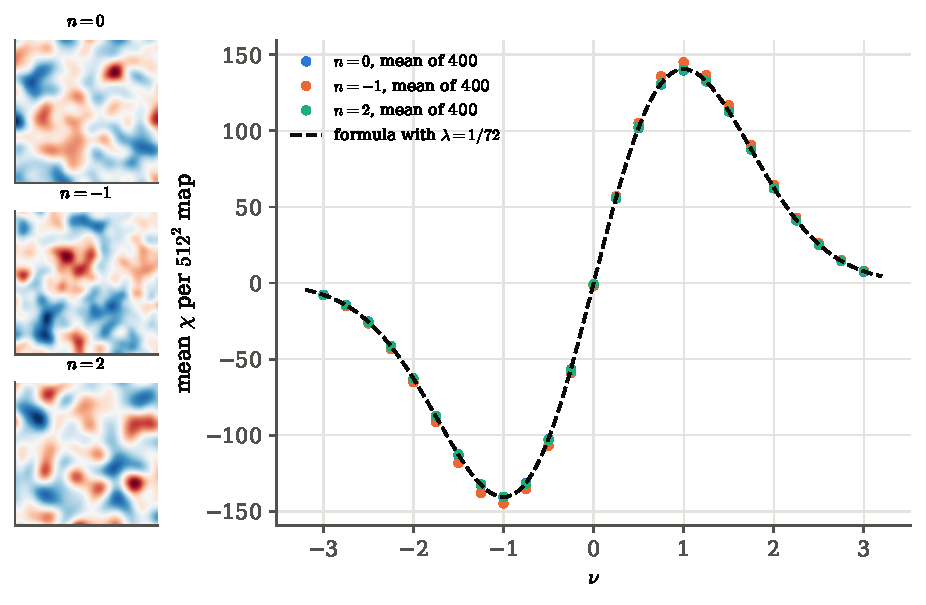
\includegraphics[width=\linewidth]{figures/ch12/gkf_lambda.pdf}
\caption{Three Gaussian fields with different spectra, $P\propto k^ne^{-k^2R^2}$ with $n=0,-1,2$, chosen to have
the same $\lambda$. Left: a $128\times128$ corner of one map of each. Right: their mean $\chi$ over $\GkfNsim$
maps of $\GkfN\times\GkfN$ pixels, all on the single prediction (dashed).}
\label{12a:fig:gkf-lambda}
\end{figure}

\paragraph{But not the same scatter.} The standard deviation of $\chi$ at $\nu=1$ for a single map is
$\GkfChiOneSd$ for $n=0$, $\GkfNMOneChiOneSd$ for $n=-1$ and $\GkfNTwoChiOneSd$ for $n=2$. The means are equal,
the spreads are not. The variance of a count of critical points depends on how critical points are
correlated with one another, which involves the whole correlation function and not only its curvature at the
origin. So for a Gaussian field the mean $\chi$ curve carries one number of the spectrum, while its
covariance carries more. Part~12c, which builds likelihoods for topological summaries, has to take the
covariance from simulations for exactly this reason: no formula as simple as \eqref{12a:eq:gkf2} exists for it.

\paragraph{Example: what the edges add.} The same $n=0$ maps, cut open into $\GkfN\times\GkfN$ squares (no
periodic gluing), have more pieces than the torus: pieces that wrapped across the seam are now counted twice,
and pieces touching an edge are no longer balanced by holes. The edge term of \eqref{12a:eq:square},
$2L\sqrt\lambda\,e^{-\nu^2/2}/2\pi$, is $\GkfEdgeTermZero$ at $\nu=0$, and the full square formula predicts
$\GkfSqZeroTh$; the squares give $\GkfSqZeroMC\pm\GkfSqZeroSe$. At $\nu=1$ the prediction is $\GkfSqOneTh$ and
the squares give $\GkfSqOneMC$ (\cref{12a:fig:gkf-edges}, left). The deficit at $\nu=0$, about one unit or one and a half
Monte Carlo errors, is of the size expected from the pixel grid along the edges, where the counting
convention matters most; we do not pursue it further. The lesson is quantitative: on a $512\times512$ map the
edges contribute as much to $\chi$ at the median as all the topology inside, and a masked sky, with its long
mask boundary, is affected even more.

\paragraph{Example: the sampling distribution of $\chi$.} The right panel of \cref{12a:fig:gkf-edges} is the
histogram of $\chi$ at $\nu=1$ over the $\GkfNsim$ torus maps. It is centred on the formula and close to a
Gaussian with standard deviation $\GkfChiOneSd$, about $6\%$ of the mean. That is the sampling distribution of
the statistic, the thing a likelihood needs (\cref{ch:03}): a single $512\times512$ map measures $\chi(1)$ to
about $6\%$, and a measured value $25$ units away from the Gaussian expectation would be a three-standard-deviation
departure. The near-Gaussian shape is no accident: $\chi$ is a sum of signed counts over many weakly
correlated regions of the map, and the central limit theorem (\cref{ch:02}) applies to such sums.

\begin{figure}[htbp]
\centering
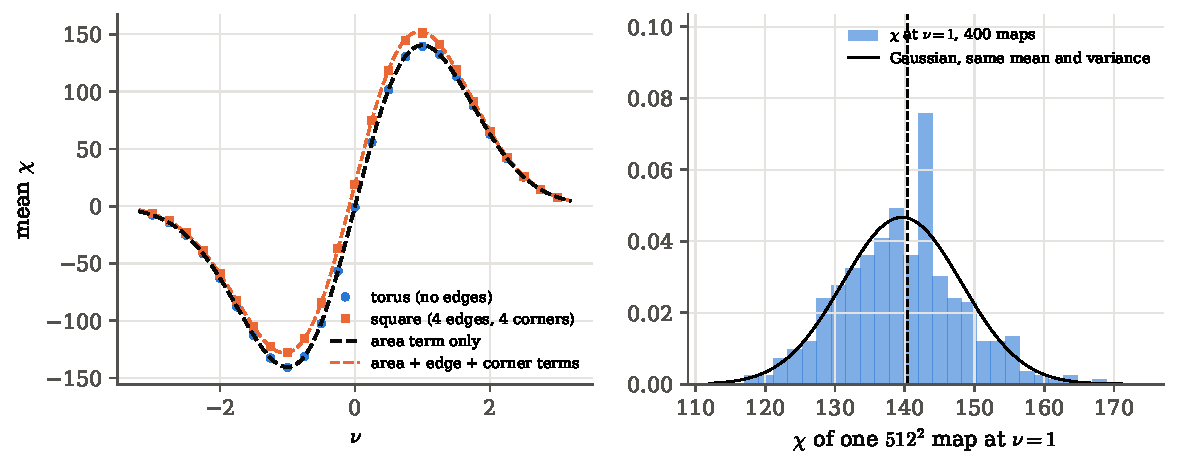
\includegraphics[width=\linewidth]{figures/ch12/gkf_edges.pdf}
\caption{Left: mean $\chi$ of the same maps on a torus (circles) and cut into squares with four edges and
four corners (squares); the black dashed line is the area term alone, the orange dashed line adds the edge and
corner terms of \eqref{12a:eq:square}. Right: the distribution of $\chi$ at $\nu=1$ over $\GkfNsim$ maps on the
torus, with a Gaussian of the same mean and variance and the predicted mean (dashed).}
\label{12a:fig:gkf-edges}
\end{figure}

\begin{inpractice}[Verification here, research instrument elsewhere]
Everything in this section is a \emph{verification}: the expected Euler characteristic of a Gaussian field is
known exactly, and the simulations test the derivation and the code against it. The same machinery becomes the
research instrument wherever no formula exists. The covariance of $\chi$ at different thresholds, the effect of
a real mask with point-source holes, of anisotropic noise, of a non-Gaussian model, of lensing followed by a
beam: none has a closed form, and analyses such as \textit{Planck}'s compare the data with large sets of
simulated skies processed by exactly the same pipeline \cite{Planck2018VII}. In that use the formula
\eqref{12a:eq:gkf} is still valuable, as the check that the pipeline reproduces the Gaussian limit before it
is trusted on anything else.
\end{inpractice}
\section{Reproducing the classic results}
\label{12a:sec:literature}

The Gaussian formula for the Euler characteristic has been derived, tested and used for forty years, in three
dimensions for the galaxy distribution, on the sphere for the microwave sky, and in a general form that also
handles weak non-Gaussianity. Four papers mark the way. Each asked a different question, set its problem up
in its own notation, and checked the answer against its own simulations. Each can be redone with the machinery of \cref{12a:sec:gkf} and our own code. Their conventions (which
variance, which normalisation, which units for the threshold) differ from paper to paper, and are the main
source of confusion when numbers are compared, so each derivation below ends by mapping their symbols to ours.

\subsection{Hamilton, Gott and Weinberg (1986): is the universe a sponge?}
\label{12a:sec:hgw}

\paragraph{Their question.} In the mid-1980s the first redshift surveys showed bubbles and walls, and three
pictures of the large-scale structure competed: isolated clusters in an empty background (``meatballs''),
empty bubbles in a connected background (``Swiss cheese''), or a ``sponge'' in which high- and low-density
regions are both connected and interlock. A Gaussian random field, the prediction of inflation, is
symmetric between overdense and underdense regions, so at the median density it must be a sponge.
Hamilton, Gott and Weinberg proposed to measure this with the curvature of the surfaces of constant
density, and derived what a Gaussian field predicts \cite{HamiltonGottWeinberg1986}.

\paragraph{Their setup.} They smooth the density contrast $\delta(\bm r)$ with a window and take the surface
$\delta=\nu\,\xi(0)^{1/2}$, where $\xi(0)$ is the variance of the smoothed field. On that surface they
integrate the Gaussian curvature $K=1/(a_1a_2)$, with $a_1,a_2$ the two principal radii of curvature at a
point. By the Gauss--Bonnet theorem the integral over one closed surface of genus $g$ (the number of handles)
is $\int K\,\dd A=4\pi(1-g)$ (their eq.~2), so a ball contributes $+4\pi$ and a doughnut $0$. Their statistic is
$C(\nu)$, the total curvature of all the surfaces per unit volume. They test it on eight simulations, each
$5\times32^3$ points laid at random in a periodic box of $32^3$ cells (so pure shot noise with no clustering),
smoothed with $W(r)=e^{-r^2/r_0^2}$ with $r_0$ twice the cell size, and they measure the curvature by tiling
space with cubes, the same idea as our voxel counting.

\paragraph{Their equation, derived.} Two facts connect $C$ to our Euler characteristic. Gauss--Bonnet for a
closed surface reads $\int K\,\dd A=2\pi\chi(\text{surface})$, and the surface bounding a solid region has twice
the Euler characteristic of the solid, $\chi(\partial X)=2\chi(X)$ (a ball: $\chi=1$, its sphere $\chi=2$; see the
topology notes). With $\E[c_3(\nu)]$ from \eqref{12a:eq:gkf3},
\begin{align}
  C(\nu)
  &\eqby{1}\frac{2\pi\,\chi(\partial X_\nu)}{V}
   \eqby{2}4\pi\,\frac{\chi(X_\nu)}{V}
   \eqby{3}4\pi\,\frac{\lambda^{3/2}}{(2\pi)^2}(\nu^2-1)e^{-\nu^2/2}
   \eqby{4}-\frac1\pi\left[\frac{-\xi''(0)}{\xi(0)}\right]^{3/2}(1-\nu^2)e^{-\nu^2/2} .
  \label{12a:eq:hgw}
\end{align}
\begin{explain}
  \item Gauss--Bonnet, summed over all the surfaces in the volume $V$.
  \item The boundary of a solid has twice its Euler characteristic.
  \item Take the expectation with \eqref{12a:eq:gkf3}.
  \item $4\pi/(4\pi^2)=1/\pi$; and for an isotropic field $-\xi''(0)/\xi(0)=\langle k^2\rangle/3=\lambda$, the
        variance of one gradient component in units of the field variance (their eq.~4).
\end{explain}
This is their eq.~(3). Symbol map: their $\xi(0)$ is our $\sigma_0^2$, their $-\xi''(0)$ our $\sigma_0^2\lambda$
in three dimensions, their genus per unit volume is $-\chi/V$. The minimum of $C$ is at $\nu=0$, where
$C=-\lambda^{3/2}/\pi$: a sponge. In their Fig.~4 they plot $C$ in units with $\lambda=1$, so the curve is
$-\pi^{-1}(1-\nu^2)e^{-\nu^2/2}$, with minimum $\HgwThZero$ and maxima $\HgwThMax$ at $\nu=\pm\sqrt3$.

\paragraph{What we compute.} The script \pyname{code/ch12/05_hgw3d.py} reproduces their setup with Poisson
counts of mean $5$ in each of the $32^3$ cells (equivalent, for this purpose, to $5\times32^3$ points dropped at
random), subtracts the mean, smooths with the Fourier transform of their window, and counts
$\chi=V-E+F-C$ of the union of closed voxels above each threshold, the three-dimensional version of
\eqref{12a:eq:vef}; on one non-periodic block the count agrees with \pyname{skimage.measure.euler_number}
($\HgwSkOk$). The result is divided by $\lambda^{3/2}$ computed from the lattice modes, $\lambda=\HgwLamThree$
(the continuum value is $1/r_0^2=0.25$):
\pyfile[firstline=36,lastline=60]{code/ch12/05_hgw3d.py}{Hamilton, Gott and Weinberg's simulation, redone}
It runs their eight simulations, then $400$ more with the same setup, then $200$ boxes of $64^3$ cells with
$r_0=4$ cells, which resolve the smoothing scale twice as finely.

\paragraph{Side by side.} \Cref{12a:fig:hgw} overlays the three runs on their curve, and the table compares
the numbers that can be read off their figure.
\begin{center}
\small
\begin{tabular}{lcccc}
\toprule
 & formula \eqref{12a:eq:hgw} & HGW Fig.~4 (read) & ours, 8 sims & ours, 400 sims \\
\midrule
$C(0)$        & $\HgwThZero$ & $-0.32$ & $\HgwEightZero\pm\HgwEightZeroSe$ & $\HgwFourZero\pm\HgwFourZeroSe$\\
$C(+1.75)$    & $\HgwThPeak$ & $0.15$  & $\HgwEightPeak$ & $\HgwFourPeak\pm0.0008$\\
$C(-1.75)$    & $\HgwThPeak$ & $0.14$  & & $\HgwFourPeakNeg\pm0.0008$\\
\bottomrule
\end{tabular}
\end{center}
Their eight simulations and ours agree with the formula, and with each other, within the scatter of eight
boxes. Their error bars are the scatter of a single box, about $0.045$ at $\nu=0$; with eight boxes the mean is
known to about $0.016$, and our eight boxes give an error of the mean of $\HgwEightZeroSe$.

\begin{figure}[htbp]
\centering
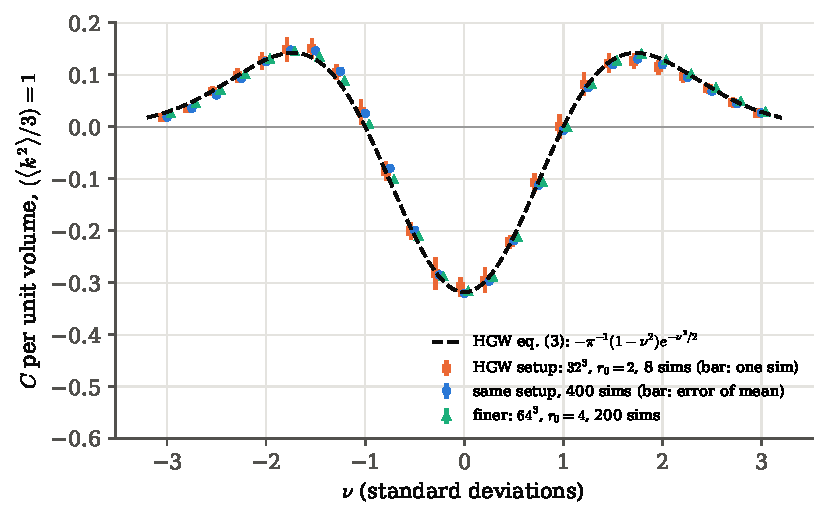
\includegraphics[width=0.78\linewidth]{figures/ch12/hgw_genus.pdf}
\caption{The total curvature of isodensity surfaces per unit volume, in units with $\lambda=1$. Dashed: the
Gaussian prediction \eqref{12a:eq:hgw}. Squares: our redo of the eight simulations of Hamilton, Gott and Weinberg
(bars: scatter of one simulation, as in their Fig.~4). Circles: $400$ simulations of the same setup (bars: error
of the mean). Triangles: $200$ finer simulations.}
\label{12a:fig:hgw}
\end{figure}

\paragraph{Why they differ.} With $400$ boxes the statistical error is small enough to look for two effects that
eight boxes hide. Hamilton, Gott and Weinberg estimated that tiling with cubes half the smoothing length biases $C(0)$
by about $1\%$. At the median our coarse boxes differ from the formula by $\HgwFourRel\%$ (a positive number means more
negative), $\HgwFourPull$ standard errors; the finer boxes differ by $\HgwFineRel\%$, $\HgwFinePull$ standard errors. A
standard error here is about half a per cent, so a $1\%$ bias sits at the edge of what $400$ boxes can see: our runs are
consistent with their estimate, but they cannot prove that the tiling is the cause. The residual non-Gaussianity of shot noise shows elsewhere, at $\nu=\pm1.75$: the coarse boxes give
$\HgwFourPeak$ at $+1.75$ and $\HgwFourPeakNeg$ at $-1.75$, against $\HgwThPeak$ for both. Shot noise is skewed
(a Poisson count has a long tail to high values), so its high peaks are fewer and broader than a Gaussian
field's and its low troughs more numerous; the curve is distorted asymmetrically. In the finer boxes each
smoothing volume holds about eight times more points, the field is closer to Gaussian, and the asymmetry
shrinks to $\HgwFinePeak$ and $\HgwFinePeakNeg$. The size and sign of this distortion is what Matsubara's
formula of \cref{12a:sec:matsubara} predicts from the skewness.

\paragraph{Lesson.} Eight simulations were enough in 1986 to show that a Gaussian field is a sponge; four
hundred show that ``Gaussian'' smoothed shot noise is not quite Gaussian, and that the genus curve is
sensitive enough to notice.

\subsection{Schmalzing and G\'orski (1998): Minkowski functionals on the sky}
\label{12a:sec:sg98}

\paragraph{Their question.} The COBE satellite had mapped the microwave sky with a $7^\circ$ beam, and the
question was whether the fluctuations were Gaussian. Schmalzing and G\'orski set out to measure all three
Minkowski functionals on the sphere, directly from pixelised maps, and asked whether their estimators
reproduce the Gaussian expectations on simulated skies \cite{SchmalzingGorski1998}.

\paragraph{Their setup.} The sky is the unit sphere, the field is the temperature $u$ in mK, and the excursion
set is $Q_\nu=\{u>\nu\}$ with the threshold $\nu$ in mK, not in units of $\sigma$. Their power spectrum is
built to look like COBE's:
\begin{center}
\small
\begin{tabular}{ll}
\toprule
ingredient & value (their eqs.~17--20)\\
\midrule
primordial spectrum & Harrison--Zel'dovich, $n=1$: $\Cell\propto1/\ell(\ell+1)$, with $C_{10}=(7\,\mu{\rm K})^2$\\
beam & Gaussian, $7^\circ$ FWHM: $g_\ell=e^{-\sigma_b^2\ell(\ell+1)/2}$, $\sigma_b=7^\circ/\sqrt{8\ln2}$\\
noise & white, $C_\ell^{\rm noise}=(3\,\mu{\rm K})^2$\\
extra smoothing & Gaussian, $e^{-\omega^2\ell(\ell+1)/2}$ with $\omega=3^\circ$\\
simulations & $1000$ skies on the $6144$ pixels of the COBE map\\
\bottomrule
\end{tabular}
\end{center}
They call the width of the extra smoothing ``$3^\circ$'' without saying whether it is $\omega$ or a FWHM. Their
Fig.~1 settles it: the smoothed noise spectrum $\ell(\ell+1)(3\,\mu{\rm K})^2e^{-\omega^2\ell(\ell+1)}$ peaks where
$\ell(\ell+1)=1/\omega^2$, at height $(3\,\mu{\rm K})^2/(e\,\omega^2)$. For $\omega=3^\circ=0.0524$\,rad this is
$\ell\approx18.6$ and $1.2\times10^{-3}\,{\rm mK}^2$, which is where their dotted curve peaks.

\paragraph{Their equation, derived.} Their eq.~(14) gives the expected functionals in terms of three numbers
measured from the map: the mean $\mu$, the variance (which they call $\sigma$, not $\sigma^2$) and
$\tau=\frac12\langle u_{;i}u_{;i}\rangle$, half the mean squared gradient. In our language $\tau/\sigma$ is exactly
$\lambda=\sigma_1^2/2\sigma_0^2$, and their threshold in standard units is $x=(\nu-\mu)/\sqrt\sigma$. Their
Euler-characteristic density is
\begin{align}
  v_2(\nu)
  &\eqby{1}\frac{\tau}{2\pi^{3/2}\sigma}\,\frac{\nu-\mu}{\sqrt{2\sigma}}\,
     \exp\Big(-\frac{(\nu-\mu)^2}{2\sigma}\Big)
   \eqby{2}\frac{\lambda}{2^{3/2}\pi^{3/2}}\;x\,e^{-x^2/2}
   \eqby{3}\frac{\lambda}{(2\pi)^{3/2}}\,x\,e^{-x^2/2} ,
  \label{12a:eq:sg-v2}
\end{align}
\begin{explain}
  \item Their eq.~(14), third line.
  \item $\tau/\sigma=\lambda$ and $(\nu-\mu)/\sqrt{2\sigma}=x/\sqrt2$.
  \item $2^{3/2}\pi^{3/2}=(2\pi)^{3/2}$.
\end{explain}
which is our \eqref{12a:eq:gkf2}. Their $v_1=\frac{\sqrt\tau}{8\sqrt\sigma}e^{-x^2/2}=\frac{\sqrt\lambda}{8}e^{-x^2/2}$
is a quarter of our length density \eqref{12a:eq:length}, and $v_0$ is $\Psi(x)$. Their eq.~(7),
$\chi=V_2+V_0/(2\pi R^2)$, is the Gauss--Bonnet split of \cref{12a:sec:turning}: on the unit sphere with
$v_j=V_j/4\pi$, $\chi=4\pi v_2+2v_0$, which is \eqref{12a:eq:sphere}.

\emph{A misprint.} Their eq.~(16) gives $\sigma=\sum_\ell(2\ell+1)\Cell$ and
$\tau=\sum_\ell(2\ell+1)\Cell\,\ell(\ell+1)/2$. Both sums lack the factor $1/4\pi$ of the addition theorem: the
variance of a map is $\sum_\ell\frac{2\ell+1}{4\pi}\Cell$ \eqref{T3a:eq:sigma0}. The slip cancels in
$\lambda=\tau/\sigma$, so the shapes and heights of $v_1$, $v_2$ and $\chi$ are unaffected. But it makes the
standard deviation $\sqrt{4\pi}\approx3.5$ times too large ($\SgSigmaBad$ instead of $\SgSigma\,\mu$K for their
spectrum) and would stretch every curve plotted against the threshold in mK by that factor. Their Fig.~2 runs
from $-0.25$ to $+0.25$ mK and its curves have died out by about $\pm0.13$\,mK, three times $\SgSigma\,\mu$K: they
used the correct variance and only the printed equation is wrong.

\paragraph{What we compute.} The script \pyname{code/ch12/06_sphere_sg98.py} builds their spectrum,
\pyfile[firstline=34,lastline=49]{code/ch12/06_sphere_sg98.py}{The COBE-like spectrum of Schmalzing and G\'orski}
\noindent draws $\SgNsim$ skies at HEALPix $N_{\rm side}=128$ ($\SgNpixFine$ pixels of $0.46^\circ$) and again at
$N_{\rm side}=32$ ($\SgNpix$ pixels of $1.8^\circ$, close to the $2.6^\circ$ COBE pixels), and measures the functionals
with the library \pyname{lib_sphere.py}: area by counting pixels; length by the band argument of
\eqref{12a:eq:length} with the gradient computed from the $\alm$; $\chi$ by $V-E+F$ of the HEALPix pixel mesh (which
pixels share each corner and each edge is worked out once from the pixel corners). As a check, $\chi$ is also
computed as pieces of the hot set (pixels touching at an edge or a corner) minus pieces of the cold set (pixels
sharing an edge) plus one, the spherical form of Alexander duality: $\beta_1$ of the hot set is the number of cold
pieces minus one, because on the sphere one cold piece is the ``outside''. In $\SgBettiChecks$ comparisons the two
counts disagree $\SgBettiBad$ times. For this spectrum $\lambda=\SgLam$\,sr$^{-1}$, a correlation angle
$\theta_c=1/\sqrt{2\lambda}=\SgThetaC^\circ$.

\paragraph{Side by side.}
\begin{center}
\small
\begin{tabular}{lccc}
\toprule
 & formula & SG98 Fig.~2 (read) & ours, $N_{\rm side}=128$ \\
\midrule
peak of $v_1$ (at $\nu=0$)            & $\SgVoneMaxTh$ & $\approx0.9$ & $\SgVoneMaxMC$\\
peak of $v_2$ [sr$^{-1}$]             & $\SgVtwoMaxTh$ & $\approx2.1$ & $\SgVtwoMaxMC$\\
$\chi$ at its peak ($\nu\approx\sigma$) & $\SgChiOneTh$ & $\approx26$  & $\SgChiOneMC\pm\SgChiOneSd$ (one sky)\\
threshold of the $\chi$ peak [mK]     & $0.041$ & $\approx0.04$ & $\SgChiPeakMK$\\
$\chi$ at $\nu=-3\sigma$              & $\SgChiMthreeTh$ & $\to2$ at low $\nu$ & $\SgChiMthreeMC$\\
\bottomrule
\end{tabular}
\end{center}
\Cref{12a:fig:sg98} is our version of their Fig.~2. The mean curves of our skies lie on the formula, the
values read from their figure sit on top of both, and the full-sky $\chi$ rises to the sphere's own value
$2$ at low thresholds, the $2v_0$ term without which the curve would go to zero (dotted).

\begin{figure}[htbp]
\centering
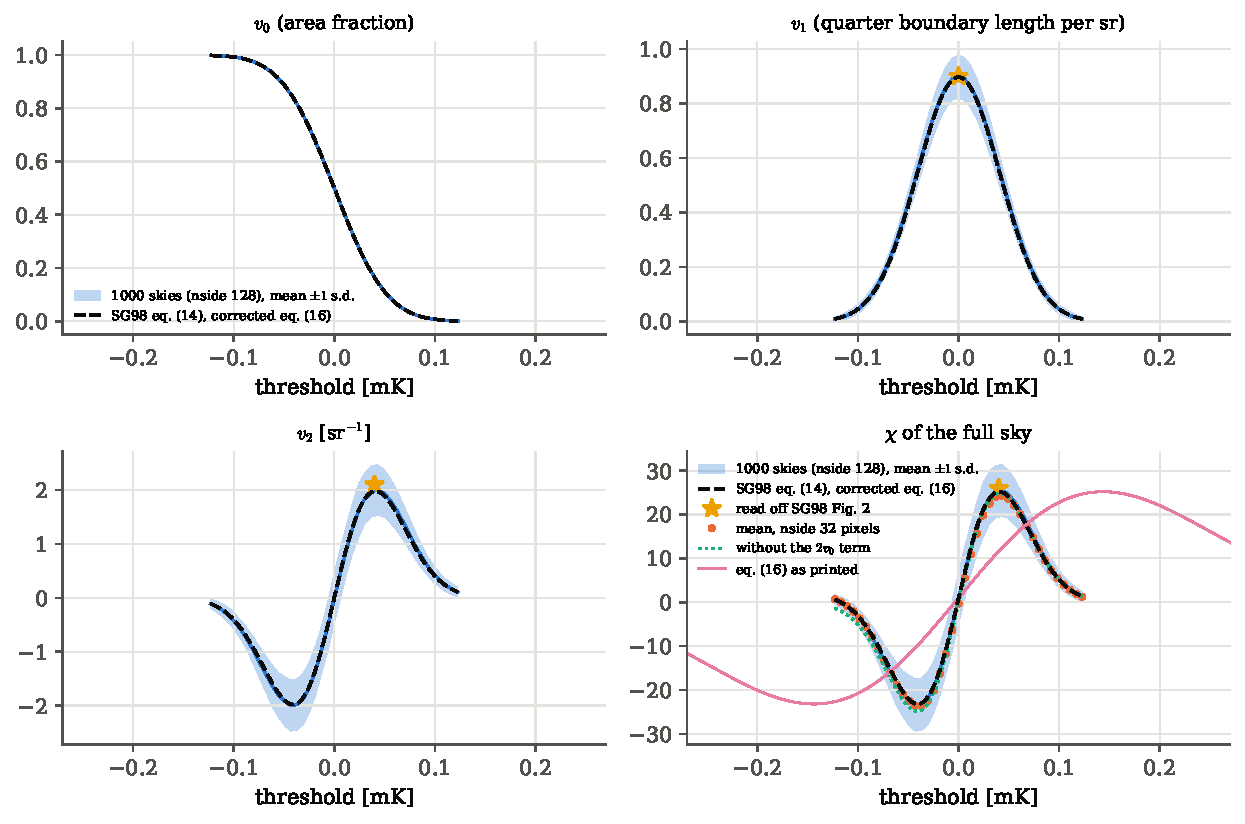
\includegraphics[width=\linewidth]{figures/ch12/sg98_mfs.pdf}
\caption{The Minkowski functionals of $\SgNsim$ COBE-like Gaussian skies against threshold in mK, as in
Schmalzing and G\'orski's Fig.~2. Band: mean $\pm$ one standard deviation of a single sky ($N_{\rm side}=128$).
Dashed: their eq.~(14) with the variance computed correctly. Stars: values read off their figure. In the $\chi$
panel, orange dots are the mean at $N_{\rm side}=32$, the dotted line omits the $2v_0$ term, and the pink line
shows what the printed eq.~(16) would give.}
\label{12a:fig:sg98}
\end{figure}

\paragraph{Why they differ.} Three effects, each small. First, pixel size: at $N_{\rm side}=32$ the pixels are a
third of the correlation angle, and counting $\chi$ on them loses $\SgCoarseDef\pm\SgCoarseDefSe\%$ at the peak
($\SgChiOneCoarse$ instead of $\SgChiOneMC$, on the same skies), because small spots and narrow necks are not resolved. Schmalzing
and G\'orski avoided this by not counting at all: their estimator integrates the curvature formula of their
eq.~(12) over pixels, using derivatives of the field, which does not care whether a spot is resolved by the
grid. Second, our thresholds are in units of each sky's own mean and standard deviation, as theirs are (their
eq.~15). Those two numbers fluctuate from sky to sky, because a sky with a $\SgThetaC^\circ$ correlation angle has
only a few hundred independent spots. Each sky's threshold scale is therefore shifted and stretched a little at
random, and averaging the curve over those random rescalings bends it slightly where it is most curved. The
largest deviation of our $1000$-sky mean from the formula is $\SgMaxPull$ Monte Carlo errors, but only
$\SgMaxDiff$ in $\chi$, at $\nu=\SgMaxPullNu$, against a scatter of several units for one sky; it would disappear
with thresholds fixed in units of the ensemble standard deviation, which a real sky does not offer. Third, the numbers read from their figure are good to about five per cent.

\paragraph{Lesson.} The formula carries over to the sphere with one extra term, the sphere's own Euler
characteristic times the area fraction; and a misprinted normalisation that cancels in every shape still
matters as soon as a curve is plotted against a physical threshold.

\subsection{Matsubara (2003): one formula for every functional}
\label{12a:sec:matsubara}

\paragraph{His question.} The Gaussian predictions are only the starting point: the late universe is not
Gaussian, and the question is how the Minkowski functionals change when it departs slightly. Matsubara
derived the Gaussian functionals and their first non-Gaussian corrections, in any dimension and for every
functional, in a single expression \cite{Matsubara2003}.

\paragraph{His equation, and ours.} For a field with variance $\sigma_0^2$ and gradient variance $\sigma_1^2$ in
$d$ dimensions, his eq.~(3.54) reads, at zeroth order in the non-Gaussianity,
\begin{equation}
  V_k^{(d)}(\nu)=\frac{1}{(2\pi)^{(k+1)/2}}\,\frac{\omega_d}{\omega_{d-k}\,\omega_k}
  \left(\frac{\sigma_1}{\sqrt d\,\sigma_0}\right)^{k}e^{-\nu^2/2}H_{k-1}(\nu),
  \qquad \omega_k=\frac{\pi^{k/2}}{\Gamma(k/2+1)},
  \label{12a:eq:matsubara}
\end{equation}
where $\omega_k$ is the volume of the unit ball in $k$ dimensions ($\omega_0=1$, $\omega_1=2$, $\omega_2=\pi$,
$\omega_3=4\pi/3$) and $H_n$ are the Hermite polynomials $H_0=1$, $H_1=\nu$, $H_2=\nu^2-1$, with
$e^{-\nu^2/2}H_{-1}(\nu)=\int_\nu^\infty e^{-t^2/2}\dd t$. Symbol map: $\sigma_1/(\sqrt d\,\sigma_0)=\sqrt\lambda$,
because $\sigma_1^2/\sigma_0^2$ is the sum of the $d$ equal gradient-component variances. Then, in the plane,
\begin{align}
  V_2^{(2)}
  &\eqby{1}\frac{1}{(2\pi)^{3/2}}\,\frac{\pi}{\omega_0\,\pi}\,\lambda\,e^{-\nu^2/2}\nu
   =\frac{\lambda}{(2\pi)^{3/2}}\,\nu e^{-\nu^2/2},
  \qquad
  V_1^{(2)}\eqby{2}\frac{1}{2\pi}\,\frac{\pi}{2\cdot2}\,\sqrt\lambda\,e^{-\nu^2/2}=\frac{\sqrt\lambda}{8}e^{-\nu^2/2},
  \nonumber\\
  V_0^{(2)}
  &\eqby{3}\frac{1}{\sqrt{2\pi}}\,\frac{\pi}{\pi\cdot1}\int_\nu^\infty e^{-t^2/2}\dd t=\Psi(\nu),
  \qquad
  V_3^{(3)}\eqby{4}\frac{1}{(2\pi)^2}\,\frac{4\pi/3}{1\cdot4\pi/3}\,\lambda^{3/2}e^{-\nu^2/2}(\nu^2-1).
  \label{12a:eq:matsubara-check}
\end{align}
\begin{explain}
  \item $k=d=2$: $\omega_2/(\omega_0\omega_2)=1$, $H_1=\nu$. This is the Euler characteristic density
        \eqref{12a:eq:gkf2}; his eq.~(3.18) for the two-dimensional genus is the same expression.
  \item $k=1$, $d=2$: $\omega_2/(\omega_1\omega_1)=\pi/4$, $H_0=1$. This is a quarter of the length density
        \eqref{12a:eq:length}, the normalisation used for $v_1$ on the sky.
  \item $k=0$: the area fraction \eqref{12a:eq:area}.
  \item $k=d=3$: the three-dimensional Euler characteristic density \eqref{12a:eq:gkf3}, $\rho_3$ of
        \eqref{12a:eq:gkf}; minus it is his three-dimensional genus.
\end{explain}
Every Gaussian result of this part is one line of \eqref{12a:eq:matsubara}, and every Monte Carlo of
\cref{12a:sec:mc,12a:sec:hgw,12a:sec:sg98} is therefore also a check of it: in two dimensions to a few tenths of a
per cent (\cref{12a:sec:mc}), in three to about one per cent (\cref{12a:sec:hgw}), on the sphere to the accuracy
of the pixel counting (\cref{12a:sec:sg98}).

\paragraph{The non-Gaussian part.} Matsubara's formula continues with a term proportional to $\sigma_0$ and to
three skewness parameters $S^{(0)},S^{(1)},S^{(2)}$, averages of $u^3$, $u^2\nabla^2u$ and
$|\nabla u|^2\nabla^2u$ \cite{Matsubara2003}; \cref{T3a:sec:matsubara} wrote it out for the sky and tested it on
skewed maps. Two features matter here. The correction is built from the Hermite polynomials $H_{k+2}$, $H_k$
and $H_{k-2}$, which are odd where the Gaussian term is even and vice versa, so it distorts the curves
asymmetrically, as the shot noise did in \cref{12a:sec:hgw}. And when the threshold is labelled by area fraction
(\cref{12a:sec:monotone}) the term with $S^{(0)}$, the one-point skewness, disappears and only the differences
$S^{(1)}-S^{(0)}$ and $S^{(2)}-S^{(0)}$ survive (his eq.~3.54 in the variable $\nu_A$). That is the perturbative
version of the exact statement of \cref{12a:sec:monotone}: relabelling removes what is in the histogram of the
values and keeps what is in their arrangement.

\paragraph{Lesson.} The four Gaussian densities are one formula. What the field contributes is a single number
per dimension, $\lambda^{k/2}$; everything else is geometry ($\omega_k$) and the Hermite polynomials.

\subsection{\textit{Planck} 2018: are the microwave sky's shapes Gaussian?}
\label{12a:sec:planck}

\paragraph{Their question.} \Cref{T3a:sec:planck-mf} described how the \textit{Planck} collaboration used the
three functionals, at many resolutions, to test whether the temperature and polarization maps are consistent
with Gaussian, isotropic skies \cite{Planck2018VII}. Here we reproduce the Gaussian side of that test, the
curves against which the data are compared (their Fig.~10), and work out in which normalisation those curves are
drawn.

\paragraph{Their setup.} The four component-separated maps are degraded to a chosen $N_{\rm side}$ and smoothed
with a Gaussian beam whose FWHM grows with the pixel size ($40'$ at $N_{\rm side}=256$, their Table~1). A common
mask leaves $75\%$ of the sky. The thresholds are $12$ values from $-3$ to $3$ in units of the map's own standard
deviation $\sigma_0$. At each threshold they compute the area fraction, the boundary length and the genus
(their eqs.~13--15), divide out the part of each that depends on the power spectrum to get what they call
``normalised'' functionals, and compare the $36$ numbers with $999$ FFP10 simulations, which contain the CMB, the noise and the component-separation
pipeline, through a $\chi^2$ with the simulation covariance (their eqs.~20--22).

\paragraph{Their equations, derived.} Their eqs.~(16)--(19) are \eqref{12a:eq:matsubara} with $d=2$:
$V_k=A_kv_k$, with $v_k=e^{-\nu^2/2}H_{k-1}(\nu)$ and
$A_k=\frac{1}{(2\pi)^{(k+1)/2}}\frac{\omega_2}{\omega_{2-k}\omega_k}\big(\frac{\sigma_1}{\sqrt2\sigma_0}\big)^k$. All
the dependence on the spectrum is in the factor $(\sigma_1/\sigma_0)^k$. Its value for their maps follows from the
sums \eqref{T3a:eq:sigma0} and \eqref{T3a:eq:sigma1} with the fiducial spectrum, the $40'$ beam and the
$N_{\rm side}=256$ pixel window: $\sigma_1/\sigma_0=\PlRatioTh$ per radian, a correlation angle
$\theta_c=\PlThetaC'$, compared with a pixel of $\PlPixArcmin'$. The genus amplitude per steradian is then
$\lambda/(2\pi)^{3/2}\approx\PlRatioTh^2/(2\times15.75)\approx370$.

\paragraph{The normalisation of their figure.} Their Fig.~10 shows the boundary length peaking at about
$\PlVoneRead$ and the genus between about $-0.020$ and $+\PlVtwoRead$, at every resolution from
$N_{\rm side}=32$ to $1024$. These cannot be the functionals per steradian (the genus amplitude above is in the
hundreds and grows with resolution), nor the normalised $v_k$ of their eq.~(17) (which peak at $1$ and
$e^{-1/2}=0.61$). They are reproduced exactly by $V_k/(\sigma_1/\sigma_0)^k$, the Gaussian functionals with the
spectral factor divided out but the numerical prefactors of $A_k$ kept:
\begin{align}
  \frac{V_1}{\sigma_1/\sigma_0}
  &\eqby{1}\frac{1}{2\pi}\,\frac{\pi}{2\cdot2}\,\frac{1}{\sqrt2}\,e^{-\nu^2/2}
   =\frac{e^{-\nu^2/2}}{8\sqrt2}\;\;\Rightarrow\;\;\text{peak }\PlVonePeakTh,
  \nonumber\\
  \frac{V_2}{(\sigma_1/\sigma_0)^2}
  &\eqby{2}\frac{1}{(2\pi)^{3/2}}\,\frac12\,\nu\,e^{-\nu^2/2}
   \;\;\Rightarrow\;\;\text{extremes }\pm\frac{e^{-1/2}}{2(2\pi)^{3/2}}=\pm0.0193 .
  \label{12a:eq:planck-norm}
\end{align}
\begin{explain}
  \item $A_1$ with $\sigma_1/\sigma_0$ set to one: $\omega_2/(\omega_1\omega_1)=\pi/4$ and
        $(1/\sqrt2)^1$.
  \item $A_2$ with $\sigma_1/\sigma_0$ set to one: $\omega_2/(\omega_0\omega_2)=1$ and $(1/\sqrt2)^2=\frac12$;
        $\nu e^{-\nu^2/2}$ is extreme at $\nu=\pm1$.
\end{explain}
At their nearest thresholds to the extremes, $\nu=\pm0.27$ for the length and $\pm0.82$ for the genus, these give
$\PlVoneTh$ and $\pm\PlVtwoTh$. Why divide out only $(\sigma_1/\sigma_0)^k$? Because it is the one factor that
changes with resolution (the beam sets $\sigma_1$) and from map to map (cosmic variance); dividing it out makes
the curves at different $N_{\rm side}$ comparable and removes most of the fluctuation of the overall amplitude,
leaving the shape, which is where non-Gaussianity would show. Their eq.~(15), read literally, would add a further
$1/2\pi$ to the genus; the plotted curves do not have it.

\paragraph{What we compute.} The script \pyname{code/ch12/07_planck_mf.py} draws $\PlNsim$ full-sky Gaussian maps
with the fiducial spectrum (\cref{ch:T1}), the $40'$ beam and the pixel window at $N_{\rm side}=256$,
$\ell\le\PlLmax$. For each map it measures $\sigma_0$ and $\sigma_1$ (from the exact derivative maps) and the
functionals at their $12$ thresholds and on a finer grid:
\pyfile[firstline=46,lastline=58]{code/ch12/07_planck_mf.py}{Planck-style normalised functionals of one map}
\noindent The measured $\sigma_1/\sigma_0$ is $\PlRatioMC\pm\PlRatioSd$ per radian against $\PlRatioTh$ from the
spectrum. Then, as \textit{Planck} does, it forms the $36$-number vector of each map, estimates the covariance from
the other $\PlNsim-1$ maps (with the Hartlap factor $\PlHartlap$ \cite{Hartlap2007}), and computes each map's $\chi^2$.

\paragraph{Side by side.}
\begin{center}
\small
\begin{tabular}{lcccc}
\toprule
 & formula & \textit{Planck} Fig.~10 & ours, & ours,\\
 & \eqref{12a:eq:planck-norm} & (read) & mean & one map\\
\midrule
length at $\nu=0.27$  & $\PlVoneTh$ & $\PlVoneRead$ & $\PlVoneMC$ & $\pm\PlVoneSd$\\
genus at $\nu=0.82$   & $\PlVtwoTh$ & $\PlVtwoRead$ & $\PlVtwoMC$ & $\pm\PlVtwoSd$\\
$\chi^2/N_{\rm dof}$, Gaussian sky & $1$ & peak near $1$ & $\PlChiMean$ (median $\PlChiMed$) & \\
\bottomrule
\end{tabular}
\end{center}

\begin{figure}[htbp]
\centering
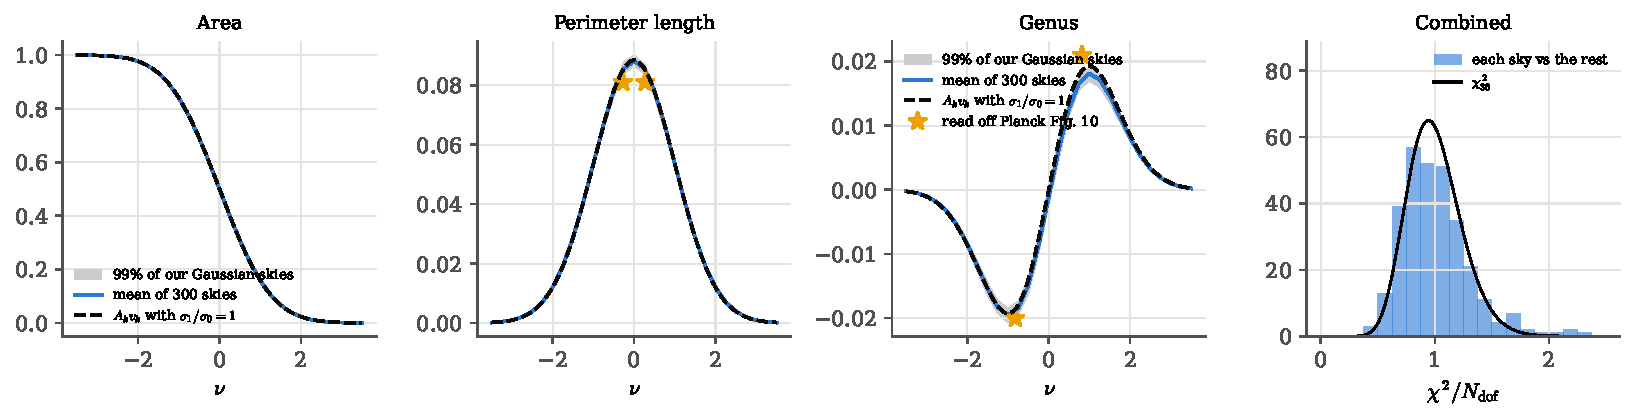
\includegraphics[width=\linewidth]{figures/ch12/planck_mf.pdf}
\caption{Our version of the $N_{\rm side}=256$ row of \textit{Planck}'s Fig.~10. Grey: the central $99\%$ of $\PlNsim$
Gaussian skies; blue: their mean; dashed: \eqref{12a:eq:planck-norm}; stars: values read off the published figure.
Right: $\chi^2/N_{\rm dof}$ of each sky against the other skies, using all $36$ numbers, with the $\chi^2_{36}$
distribution.}
\label{12a:fig:planck}
\end{figure}

\paragraph{Why they differ.} The length agrees with the formula to the third digit and with the published curve
to within the accuracy of reading it. The genus of our maps is $\PlVtwoMC$, about $7\%$ below the formula. That is
the pixel effect of \cref{12a:sec:pixels}, now large because the correlation angle is only $2.3$ pixels. Its
signature is clearest at the median: the full-sky $\chi$ at $\nu=0$ should be $2\Psi(0)=1$, and our skies give
$\PlChiZero\pm\PlChiZeroSe$. Near $\nu=0$ the expected $\chi$ rises with slope $4\pi\lambda/(2\pi)^{3/2}=\PlChiSlope$ per
unit of $\nu$, so this is the whole curve shifted by $\PlShift$ standard deviations towards higher thresholds. The
8-neighbour rule joins hot pixels that touch at a corner, which makes the hot set behave as if the threshold were
slightly lower at every saddle that falls inside a $2\times2$ block of pixels; the effect is as large as the fraction
of saddles that are not resolved by the grid. The same skies sampled at $N_{\rm side}=512$ give a genus of
$\PlVtwoFiveOneTwo$ instead of $\PlVtwoTwoFiveSix$ at $\nu=0.82$, a deficit of $\PlPixDef\%$ that finer pixels mostly
remove. The published curve, read at $\approx\PlVtwoRead$, lies about $10\%$ above the formula.
We cannot settle the reason from the paper: their genus is computed from counts of hot and cold spots on the
masked sky with their own pixel treatment, and the reading of a small figure is uncertain at this level. It does not
matter for their test, and this is the point of their method: data and simulations pass through the identical
estimator, so any such offset is common to both and cancels in the comparison. Finally, the $\chi^2$ of Gaussian skies
against Gaussian skies follows the $\chi^2_{36}$ distribution, mean $\PlChiMean$ per degree of freedom, which is what the
histograms of their right-hand column show for the FFP10 simulations.

\paragraph{Lesson.} A published curve is only reproducible once its normalisation is reverse-engineered; here the
curves are the Gaussian functionals with $\sigma_1/\sigma_0$ divided out. And the reason the \textit{Planck} test is
robust to such details is that it never compares the data with a formula, only with simulations processed the same
way.
\section{How it is done in research}
\label{12a:sec:research}

The calculations so far used clean, full-sky or periodic Gaussian maps, because that is where the answer is
known and the code can be checked. A real analysis of the microwave sky starts from maps that have been
through an instrument and a foreground-cleaning pipeline, covers only part of the sky, and asks whether the
measured curves are consistent with a model whose only complete description is a set of simulations. The
pipeline of the \textit{Planck} temperature and polarization analysis \cite{Planck2018VII} runs as follows,
each step with its purpose.

\paragraph{The data products.} Four maps of the CMB, each produced by a different component-separation method
(Commander, NILC, SEVEM, SMICA), at $N_{\rm side}=2048$; for each, a common mask of the Galaxy and point
sources; and $999$ FFP10 simulations, which are Gaussian CMB skies from the best-fit spectrum, lensed, observed
with the real scanning, beams and noise, and passed through the same component separation. The simulations
are the null hypothesis: a sky that is Gaussian and isotropic apart from everything the instrument and the
pipeline do to it.

\paragraph{The pipeline.}
\begin{enumerate}[itemsep=2pt,leftmargin=1.5em]
  \item \emph{Choose a resolution.} Degrade each map to $N_{\rm side}$ between $16$ and $2048$ and smooth it with a
        Gaussian beam whose FWHM is about three pixels (their Table~1). The smoothing makes the field smooth on the
        pixel scale, which the counting needs (\cref{12a:sec:pixels}), and fixes $\sigma_1/\sigma_0$. Each
        resolution probes a different range of scales.
  \item \emph{Apply the mask.} Only unmasked pixels enter. The mask's boundary adds pieces to the excursion set
        and changes $\chi$ (\cref{12a:sec:edges}); because the simulations are masked identically, the effect is
        carried by the null distribution rather than modelled.
  \item \emph{Set the thresholds.} Twelve thresholds from $-3$ to $3$, in units of the standard deviation measured
        on the unmasked part of the map itself.
  \item \emph{Measure.} The area fraction by counting pixels, the boundary length from the contour lengths, the
        genus from the numbers of hot and cold spots; then divide by $(\sigma_1/\sigma_0)^k$
        (\cref{12a:sec:planck}).
  \item \emph{Repeat on every simulation}, with the identical code, to obtain the sampling distribution of the
        $36$ numbers.
  \item \emph{Compare.} Form the $\chi^2$ of the data vector with the mean and covariance of the simulations; the
        $p$-value is the fraction of simulations with a larger $\chi^2$ (their Table~5). Repeat for each resolution,
        for each component-separation method, and for $E$-mode polarization.
\end{enumerate}

\begin{figure}[htbp]
\centering
\begin{tikzpicture}[
  bx/.style={draw=accent,thick,rounded corners=2pt,fill=ideabg,font=\small,
             minimum height=10mm,align=center,text width=27mm},
  sb/.style={bx,draw=tangentgreen!80!black},
  rb/.style={bx,draw=bdryred!80!black},
  flow/.style={->,thick,accent}]
  \node[bx] (map) at (0,0)     {data map\\ (4 methods)};
  \node[sb] (sim) at (0,-2.1)  {999 FFP10\\ simulations};
  \node[bx] (deg) at (3.6,-1.05) {degrade, smooth,\\ mask};
  \node[bx] (thr) at (7.2,-1.05) {thresholds in\\ units of $\sigma_0$};
  \node[bx] (mf)  at (10.8,-1.05) {$v_0,v_1,v_2$ at 12\\ thresholds};
  \node[sb] (cov) at (10.8,-3.3) {mean and\\ covariance};
  \node[rb] (chi) at (7.2,-3.3)  {$\chi^2$ and\\ $p$-value};
  \draw[flow] (map) -- (deg);
  \draw[flow] (sim) -- (deg);
  \draw[flow] (deg) -- (thr);
  \draw[flow] (thr) -- (mf);
  \draw[flow] (mf) -- (cov);
  \draw[flow] (cov) -- (chi);
  \draw[flow] (mf.south west) to[out=-120,in=60] (chi.north);
\end{tikzpicture}
\caption{The Minkowski-functional test of a sky map. Data and simulations follow the same path; the
simulations (green) provide the mean and covariance of the $36$ numbers, against which the data vector is
compared through a $\chi^2$ (red).}
\label{12a:fig:pipeline}
\end{figure}

\paragraph{The checks.} Each step has a failure mode, and a real analysis tests for it before looking at the
data. The Gaussian limit: on Gaussian simulations without mask the pipeline must reproduce the formulas of
\cref{12a:sec:gkf}, which is what \cref{12a:sec:mc,12a:sec:sg98,12a:sec:planck} did. Convergence: the covariance
of $36$ numbers from $999$ simulations is well determined, but its inverse is biased by the factor
$(n-p-2)/(n-1)$ \cite{Hartlap2007}, $0.96$ for $n=999$ and $p=36$; with fewer simulations, or more thresholds, the
correction grows quickly. Resolution and convention: the counts must be stable when the pixel size is halved at
fixed smoothing (our genus moved by $\PlPixDef\%$ at $N_{\rm side}=256$, \cref{12a:sec:planck}), and the connectivity
convention must be the same for data and simulations. The mask: the counts near the mask boundary are the most
fragile, and their effect is checked by changing the mask. Agreement between the four component-separation
methods is itself a test of foreground residuals.

\subsection{What a mask does, and how the formula absorbs it}
\label{12a:sec:mask}

The general formula \eqref{12a:eq:gkf} says that a mask enters only through three numbers of the unmasked
region: its Euler characteristic $\mathcal L_0$, half its boundary length $\mathcal L_1$ and its area
$\mathcal L_2$. A tempting shortcut, ``the masked sky is a fraction $\fsky$ of the full sky, so multiply the
full-sky prediction by $\fsky$'', misses the boundary term entirely. How much does that matter?

\paragraph{Example: a Galactic band.} The script \pyname{code/ch12/08_mask_gkf.py} masks the band
$|b|<\MkBcut^\circ$ around the Galactic equator, leaving two polar caps of angular radius $70^\circ$
($\fsky=\MkFsky\%$). For two caps, $\mathcal L_0=2$ (two discs), $\mathcal L_1$ is half of the two boundary circles,
$\frac12\cdot2\cdot2\pi\sin70^\circ=\MkLone$, and $\mathcal L_2$ is their area, $2\cdot2\pi(1-\cos70^\circ)=\MkLtwo$\,sr.
On $\MkNsim$ Gaussian skies with the fiducial spectrum, a $\MkFwhm'$ beam and $N_{\rm side}=\MkNside$
($\lambda=\MkLam$\,sr$^{-1}$, a correlation angle of about nine pixels, so that the pixel shift found in
\cref{12a:sec:planck} is negligible), standardised on the unmasked pixels, the mean $\chi$ of the unmasked excursion set at
$\nu=0$ is $\MkZeroMC\pm\MkZeroSe$. The formula with the three $\mathcal L_j$ predicts $\MkZeroTh$, of which the boundary
term $\mathcal L_1\rho_1(0)$ is $\MkEdgeZero$; the $\fsky$ shortcut predicts $\MkZeroNaive$. At $\nu=1$ the skies give
$\MkOneMC$, the formula $\MkOneTh$, the shortcut $\MkOneNaive$ (\cref{12a:fig:mask}). The largest deviation of the
simulated mean from the formula, over all thresholds, is $\MkMaxPull$ Monte Carlo errors, a few per cent of the
peak value of $\chi$: the residual of the pixel counting and of standardising each sky on its own unmasked pixels. So the boundary of a
simple mask adds a known, sizeable amount to $\chi$, and the formula accounts for it exactly; a real mask, with
hundreds of point-source holes each adding its own boundary, makes $\mathcal L_1$ large and is one reason real
analyses rely on simulations masked in the same way.

\begin{figure}[htbp]
\centering
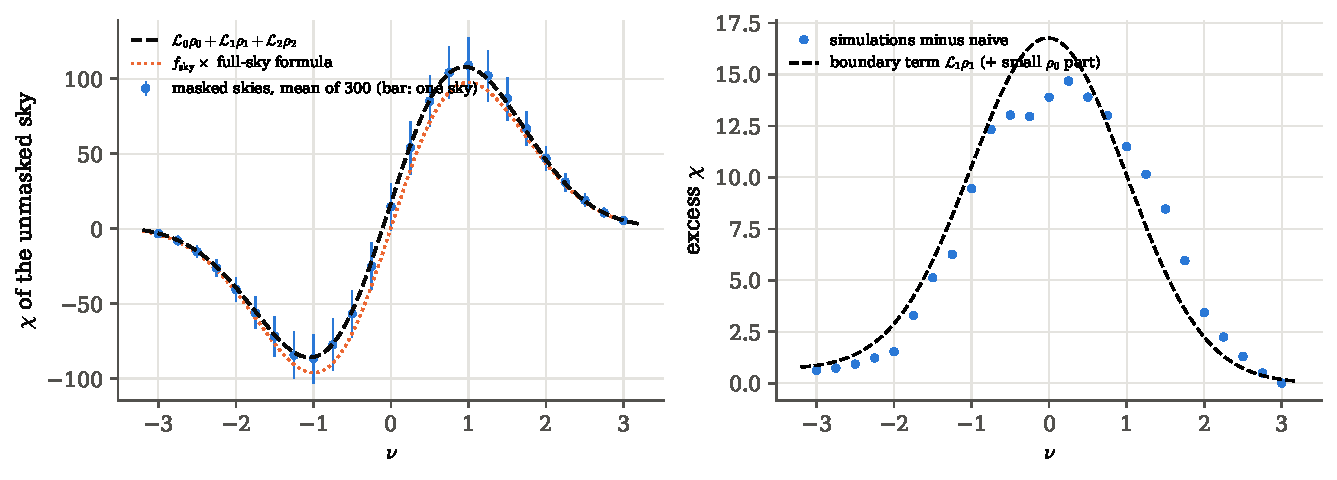
\includegraphics[width=\linewidth]{figures/ch12/mask_gkf.pdf}
\caption{Euler characteristic of the sky outside a $|b|<\MkBcut^\circ$ band. Left: the mean over $\MkNsim$
Gaussian skies (bars: one sky), the formula with the Lipschitz--Killing numbers of the two caps (dashed) and the
full-sky formula scaled by $\fsky$ (dotted). Right: the difference between the simulations and the $\fsky$
shortcut is the boundary term.}
\label{12a:fig:mask}
\end{figure}

\paragraph{Laptop scale, and what it costs.} Every computation in this part was reduced to run in minutes on a
laptop. Each reduction, and what the full analysis does instead:
\begin{itemize}[itemsep=1pt,leftmargin=1.2em]
  \item \textit{Planck} analyses maps up to $N_{\rm side}=2048$ with $999$ end-to-end simulations including noise,
        lensing and component separation; we used $\PlNsim$ Gaussian skies at $N_{\rm side}=256$ without noise, which
        reproduces the Gaussian curves and the $\chi^2$ distribution but cannot test foreground residuals or noise
        inhomogeneity.
  \item \textit{Planck} masks $25\%$ of the sky with a mask full of point-source holes; we used the full sky for the
        reproduction and a simple band for the mask test, which shows the boundary term but understates its size
        for a real mask.
  \item Our flat maps are $512\times512$ pixels with $400$ realisations per spectrum; this resolves the mean $\chi$
        to about $0.3\%$, enough to see the edge term and the lattice value of $\lambda$, not enough to study the
        far tails beyond $|\nu|\approx3$.
  \item Our three-dimensional boxes are $32^3$ and $64^3$ cells, where cosmic-web studies use $512^3$ or more; the
        small boxes reproduce the Gaussian genus curve but resolve only a few correlation lengths per side, so
        the residual shot-noise skewness is larger than in a large survey.
\end{itemize}

\begin{recap}
\begin{itemize}
  \item A nuisance is an operator $\phi\to\mathcal N[\phi]$; a statistic $T$ is protected if
        $T[\mathcal N[\phi]]=T[\phi]$. Counts of pieces and holes are protected against smooth one-to-one
        remappings (lensing, to first order) and monotone changes of the values; not against noise, smoothing,
        tearing, or a feature crossing a mask edge.
  \item The topology of a field is the topology of its excursion sets $X_\nu=\{\phi>\nu\}$. In two dimensions
        $\beta_0$ counts pieces, $\beta_1$ holes, and $\chi=\beta_0-\beta_1$.
  \item On pixels, use dual connectivity (8 for the set, 4 for its complement, or the reverse); $\chi=V-E+F$ of
        the closed-pixel complex equals $\beta_0-\beta_1$; labelling, cell counting, \pyname{scikit-image} and
        \pyname{gudhi} agree exactly.
  \item Under a monotone transform the excursion sets are the same sets with relabelled thresholds; labelling
        thresholds by area fraction removes all pointwise (one-point) non-Gaussianity and keeps only spatial
        information.
  \item The Minkowski functionals (area, length, $\chi$) are the complete set of additive, motion-invariant shape
        measures; $\chi$ is the total turning of the boundary over $2\pi$, plus enclosed curvature on a curved sky.
  \item Counting critical points with the sign of $\det H$ gives, for a Gaussian field,
        $\E[\chi]/A=\lambda\nu e^{-\nu^2/2}/(2\pi)^{3/2}$ with $\lambda=\sigma_1^2/2\sigma_0^2$; in 3-D
        $\lambda^{3/2}(\nu^2-1)e^{-\nu^2/2}/(2\pi)^2$; edges, masks and the sphere enter through
        $\E\chi=\sum_j\mathcal L_j\rho_j$.
  \item For a Gaussian field the mean $\chi$ curve knows only $\lambda$; its covariance knows more. A departure from
        the shape $\nu e^{-\nu^2/2}$ is a model-independent sign of non-Gaussianity.
  \item Reproduced: Hamilton--Gott--Weinberg's sponge (to $1\%$), Schmalzing--G\'orski's sky functionals (and their
        misprinted eq.~16), Matsubara's general formula, and \textit{Planck}'s Gaussian curves, whose plotted
        normalisation is $V_k/(\sigma_1/\sigma_0)^k$.
\end{itemize}
\end{recap}
\providecommand{\PbGrfN}{}\renewcommand{\PbGrfN}{256}
\providecommand{\PbGrfR}{}\renewcommand{\PbGrfR}{4}
\providecommand{\PbGrfNzero}{}\renewcommand{\PbGrfNzero}{207}
\providecommand{\PbGrfNone}{}\renewcommand{\PbGrfNone}{231}
\providecommand{\PbGrfdBgudhi}{}\renewcommand{\PbGrfdBgudhi}{0}
\providecommand{\PbGrfdBripser}{}\renewcommand{\PbGrfdBripser}{1.115\times10^{-7}}
\providecommand{\PbGrfMismatch}{}\renewcommand{\PbGrfMismatch}{0}
\providecommand{\PbGrfMonotone}{}\renewcommand{\PbGrfMonotone}{yes}
\providecommand{\PbTimeOurs}{}\renewcommand{\PbTimeOurs}{1.083}
\providecommand{\PbTimeGudhi}{}\renewcommand{\PbTimeGudhi}{0.09193}
\providecommand{\PbTimeOursBig}{}\renewcommand{\PbTimeOursBig}{15.83}
\providecommand{\PbTimeGudhiBig}{}\renewcommand{\PbTimeGudhiBig}{1.757}
\providecommand{\PbTimeSlope}{}\renewcommand{\PbTimeSlope}{1.001}
\providecommand{\PbGrfMaxPers}{}\renewcommand{\PbGrfMaxPers}{3.427}
\providecommand{\PbGrfShortFrac}{}\renewcommand{\PbGrfShortFrac}{0.3738}
\providecommand{\PbStabTrials}{}\renewcommand{\PbStabTrials}{60}
\providecommand{\PbStabCheck}{}\renewcommand{\PbStabCheck}{0}
\providecommand{\PbStabMaxRatio}{}\renewcommand{\PbStabMaxRatio}{0.9132}
\providecommand{\PbStabEps}{}\renewcommand{\PbStabEps}{0.908}
\providecommand{\PbStabAmp}{}\renewcommand{\PbStabAmp}{0.2}
\providecommand{\PbStabNclean}{}\renewcommand{\PbStabNclean}{60}
\providecommand{\PbStabNnoisy}{}\renewcommand{\PbStabNnoisy}{871}
\providecommand{\PbStabNshort}{}\renewcommand{\PbStabNshort}{863}
\providecommand{\PbStabNsmooth}{}\renewcommand{\PbStabNsmooth}{57}
\providecommand{\PbStabLongClean}{}\renewcommand{\PbStabLongClean}{3.117}
\providecommand{\PbStabLongNoisy}{}\renewcommand{\PbStabLongNoisy}{3.763}
\providecommand{\PbStabTenthClean}{}\renewcommand{\PbStabTenthClean}{1.502}
\providecommand{\PbStabTenthNoisy}{}\renewcommand{\PbStabTenthNoisy}{1.614}
\providecommand{\PbCloudNc}{}\renewcommand{\PbCloudNc}{40}
\providecommand{\PbCloudNk}{}\renewcommand{\PbCloudNk}{12}
\providecommand{\PbCloudN}{}\renewcommand{\PbCloudN}{52}
\providecommand{\PbLoopBirth}{}\renewcommand{\PbLoopBirth}{0.7001}
\providecommand{\PbLoopDeath}{}\renewcommand{\PbLoopDeath}{1.668}
\providecommand{\PbLoopSecond}{}\renewcommand{\PbLoopSecond}{0.00431}
\providecommand{\PbGapEdge}{}\renewcommand{\PbGapEdge}{1.233}
\providecommand{\PbTimeKruskal}{}\renewcommand{\PbTimeKruskal}{5.259\times10^{-4}}
\providecommand{\PbTimeBrute}{}\renewcommand{\PbTimeBrute}{0.3344}
\providecommand{\PbdBbrute}{}\renewcommand{\PbdBbrute}{2.129\times10^{-8}}
\providecommand{\PbdBgudhi}{}\renewcommand{\PbdBgudhi}{2.129\times10^{-8}}
\providecommand{\PbSimplices}{}\renewcommand{\PbSimplices}{23478}
\providecommand{\PbTimeKruskalBig}{}\renewcommand{\PbTimeKruskalBig}{0.23}
\providecommand{\PbTimeRipserBig}{}\renewcommand{\PbTimeRipserBig}{1.394}
\providecommand{\PbCloudBig}{}\renewcommand{\PbCloudBig}{1600}
\providecommand{\PbWebN}{}\renewcommand{\PbWebN}{80}
\providecommand{\PbWebCheck}{}\renewcommand{\PbWebCheck}{0}
\providecommand{\PbWebR}{}\renewcommand{\PbWebR}{2.5}
\providecommand{\PbWebBoxes}{}\renewcommand{\PbWebBoxes}{24}
\providecommand{\PbWebPeakZero}{}\renewcommand{\PbWebPeakZero}{1.7}
\providecommand{\PbWebPeakOne}{}\renewcommand{\PbWebPeakOne}{0}
\providecommand{\PbWebPeakTwo}{}\renewcommand{\PbWebPeakTwo}{-1.6}
\providecommand{\PbWebAmpZero}{}\renewcommand{\PbWebAmpZero}{0.0979}
\providecommand{\PbWebAmpOne}{}\renewcommand{\PbWebAmpOne}{0.2345}
\providecommand{\PbWebAmpTwo}{}\renewcommand{\PbWebAmpTwo}{0.1072}
\providecommand{\PbWebChiZero}{}\renewcommand{\PbWebChiZero}{-0.22}
\providecommand{\PbWebChiPeak}{}\renewcommand{\PbWebChiPeak}{0.09082}
\providecommand{\PbWebBzeroAtZero}{}\renewcommand{\PbWebBzeroAtZero}{0.00651}
\providecommand{\PbWebBtwoAtZero}{}\renewcommand{\PbWebBtwoAtZero}{0.007975}
\providecommand{\PbWebChiDev}{}\renewcommand{\PbWebChiDev}{2.205}
\providecommand{\PbWebChiErr}{}\renewcommand{\PbWebChiErr}{2.772}
\providecommand{\PbWebChiPull}{}\renewcommand{\PbWebChiPull}{1.8}
\providecommand{\PbWebChiNpull}{}\renewcommand{\PbWebChiNpull}{71}
\providecommand{\PbPoisNg}{}\renewcommand{\PbPoisNg}{64}
\providecommand{\PbPoisK}{}\renewcommand{\PbPoisK}{5}
\providecommand{\PbPoisPeakZero}{}\renewcommand{\PbPoisPeakZero}{3.833}
\providecommand{\PbPoisPeakOne}{}\renewcommand{\PbPoisPeakOne}{1.567}
\providecommand{\PbPoisPeakTwo}{}\renewcommand{\PbPoisPeakTwo}{0.9667}
\providecommand{\PbPoisSpread}{}\renewcommand{\PbPoisSpread}{0.1}
\providecommand{\PbRmSide}{}\renewcommand{\PbRmSide}{10}
\providecommand{\PbRmN}{}\renewcommand{\PbRmN}{512}
\providecommand{\PbRmFwhm}{}\renewcommand{\PbRmFwhm}{10}
\providecommand{\PbRmPix}{}\renewcommand{\PbRmPix}{1.172}
\providecommand{\PbRmReal}{}\renewcommand{\PbRmReal}{6}
\providecommand{\PbRmNzero}{}\renewcommand{\PbRmNzero}{919}
\providecommand{\PbRmMatchLow}{}\renewcommand{\PbRmMatchLow}{99.82}
\providecommand{\PbRmRuleLow}{}\renewcommand{\PbRmRuleLow}{99.66}
\providecommand{\PbRmExtraLow}{}\renewcommand{\PbRmExtraLow}{-0.07254}
\providecommand{\PbRmFirstFold}{}\renewcommand{\PbRmFirstFold}{0.3}
\providecommand{\PbRmExtraHigh}{}\renewcommand{\PbRmExtraHigh}{15.6}
\providecommand{\PbRmFoldHigh}{}\renewcommand{\PbRmFoldHigh}{22.73}
\providecommand{\PbRmMatchHigh}{}\renewcommand{\PbRmMatchHigh}{95.72}
\providecommand{\PbRmRuleHigh}{}\renewcommand{\PbRmRuleHigh}{95.48}
\providecommand{\PbRmConsHigh}{}\renewcommand{\PbRmConsHigh}{93.99}
\providecommand{\PbRmConsLow}{}\renewcommand{\PbRmConsLow}{99.43}
\providecommand{\PbRmInFoldHigh}{}\renewcommand{\PbRmInFoldHigh}{7.209}
\providecommand{\PbRmConsMin}{}\renewcommand{\PbRmConsMin}{84.31}
\providecommand{\PbNoiseRawFive}{}\renewcommand{\PbNoiseRawFive}{1.243}
\providecommand{\PbNoiseRawTwenty}{}\renewcommand{\PbNoiseRawTwenty}{5.015}
\providecommand{\PbNoiseSmFive}{}\renewcommand{\PbNoiseSmFive}{1.001}
\providecommand{\PbNoiseSmTwenty}{}\renewcommand{\PbNoiseSmTwenty}{1.005}
\providecommand{\PbNoiseMatchSmTwenty}{}\renewcommand{\PbNoiseMatchSmTwenty}{94.29}
\providecommand{\PbNoiseMatchRawTwenty}{}\renewcommand{\PbNoiseMatchRawTwenty}{37.05}
\providecommand{\PbHvh}{}\renewcommand{\PbHvh}{0.6506}
\providecommand{\PbHvFormHundred}{}\renewcommand{\PbHvFormHundred}{5245}
\providecommand{\PbHvFormFiveHundred}{}\renewcommand{\PbHvFormFiveHundred}{138531}
\providecommand{\PbHvNoreionHundred}{}\renewcommand{\PbHvNoreionHundred}{6082}
\providecommand{\PbHvNoreionFiveHundred}{}\renewcommand{\PbHvNoreionFiveHundred}{139047}
\providecommand{\PbHvNoreionFifty}{}\renewcommand{\PbHvNoreionFifty}{1659}
\providecommand{\PbHvFormFifty}{}\renewcommand{\PbHvFormFifty}{716}
\providecommand{\PbFidFormHundred}{}\renewcommand{\PbFidFormHundred}{5311}
\providecommand{\PbFidFormFiveHundred}{}\renewcommand{\PbFidFormFiveHundred}{133373}
\providecommand{\PbHvSimHundred}{}\renewcommand{\PbHvSimHundred}{6142}
\providecommand{\PbHvSimFiveHundred}{}\renewcommand{\PbHvSimFiveHundred}{137854}
\providecommand{\PbHvSimErrHundred}{}\renewcommand{\PbHvSimErrHundred}{127}
\providecommand{\PbHvSimErrFiveHundred}{}\renewcommand{\PbHvSimErrFiveHundred}{513}
\providecommand{\PbHvRatioHundred}{}\renewcommand{\PbHvRatioHundred}{1.144}
\providecommand{\PbHvRatioFiveHundred}{}\renewcommand{\PbHvRatioFiveHundred}{1.083}
\providecommand{\PbHvSlope}{}\renewcommand{\PbHvSlope}{2.123}
\providecommand{\PbHvSide}{}\renewcommand{\PbHvSide}{30}
\providecommand{\PbHvNsim}{}\renewcommand{\PbHvNsim}{12}
\providecommand{\PbHvGridDev}{}\renewcommand{\PbHvGridDev}{4.663}
\providecommand{\PbHvGridPull}{}\renewcommand{\PbHvGridPull}{2.3}
\providecommand{\PbQnside}{}\renewcommand{\PbQnside}{256}
\providecommand{\PbQnmap}{}\renewcommand{\PbQnmap}{100}
\providecommand{\PbNuHundred}{}\renewcommand{\PbNuHundred}{0.5305}
\providecommand{\PbNuFiveHundred}{}\renewcommand{\PbNuFiveHundred}{0.5273}
\providecommand{\PbNuErrHundred}{}\renewcommand{\PbNuErrHundred}{0.01527}
\providecommand{\PbNuErrFiveHundred}{}\renewcommand{\PbNuErrFiveHundred}{0.009313}
\providecommand{\PbNuDiffFive}{}\renewcommand{\PbNuDiffFive}{0.08}
\providecommand{\PbNuPullFive}{}\renewcommand{\PbNuPullFive}{5.7}
\providecommand{\PbNuPullHundred}{}\renewcommand{\PbNuPullHundred}{0.5}
\providecommand{\PbSigLowHundred}{}\renewcommand{\PbSigLowHundred}{0.1581}
\providecommand{\PbSigHighHundred}{}\renewcommand{\PbSigHighHundred}{2.436}
\providecommand{\PbSigLowFiveHundred}{}\renewcommand{\PbSigLowFiveHundred}{0.3808}
\providecommand{\PbSigHighFiveHundred}{}\renewcommand{\PbSigHighFiveHundred}{4.656}
\providecommand{\PbQside}{}\renewcommand{\PbQside}{40}
\providecommand{\PbQncen}{}\renewcommand{\PbQncen}{40}
\providecommand{\PbNuFlatHundred}{}\renewcommand{\PbNuFlatHundred}{0.4567}
\providecommand{\PbNuFlatFiveHundred}{}\renewcommand{\PbNuFlatFiveHundred}{0.4967}
\providecommand{\PbNuShufHundred}{}\renewcommand{\PbNuShufHundred}{0.8951}
\providecommand{\PbNuShufFiveHundred}{}\renewcommand{\PbNuShufFiveHundred}{0.9041}
\providecommand{\PbNNsame}{}\renewcommand{\PbNNsame}{2.404}
\providecommand{\PbNNopp}{}\renewcommand{\PbNNopp}{1.839}
\providecommand{\PbNNall}{}\renewcommand{\PbNNall}{1.684}
\providecommand{\PbNNcount}{}\renewcommand{\PbNNcount}{9110}
\providecommand{\PbNNratio}{}\renewcommand{\PbNNratio}{1.307}
\providecommand{\PbNNdensity}{}\renewcommand{\PbNNdensity}{0.1423}
\providecommand{\PbNNrandom}{}\renewcommand{\PbNNrandom}{1.325}
\providecommand{\PbWtNsim}{}\renewcommand{\PbWtNsim}{60}
\providecommand{\PbWtSame}{}\renewcommand{\PbWtSame}{-0.4781}
\providecommand{\PbWtOpp}{}\renewcommand{\PbWtOpp}{-0.07559}
\providecommand{\PbWtAll}{}\renewcommand{\PbWtAll}{-0.276}
\providecommand{\PbWtSameErr}{}\renewcommand{\PbWtSameErr}{0.005635}
\providecommand{\PbWtOppErr}{}\renewcommand{\PbWtOppErr}{0.007006}
\providecommand{\PbWtAllErr}{}\renewcommand{\PbWtAllErr}{0.005009}
\providecommand{\PbWtFarMax}{}\renewcommand{\PbWtFarMax}{0.006497}
\providecommand{\PbWtFarSigma}{}\renewcommand{\PbWtFarSigma}{4.379}
\providecommand{\TcPatchCount}{}\renewcommand{\TcPatchCount}{76}
\providecommand{\TcPatchPlus}{}\renewcommand{\TcPatchPlus}{38}
\providecommand{\TcPatchMinus}{}\renewcommand{\TcPatchMinus}{38}
\providecommand{\TcNsim}{}\renewcommand{\TcNsim}{200}
\providecommand{\TcPred}{}\renewcommand{\TcPred}{1510}
\providecommand{\TcMean}{}\renewcommand{\TcMean}{1501}
\providecommand{\TcSd}{}\renewcommand{\TcSd}{39}
\providecommand{\TcSdPoisson}{}\renewcommand{\TcSdPoisson}{39}
\providecommand{\TcSdErr}{}\renewcommand{\TcSdErr}{2}
\providecommand{\TcMeanDevPct}{}\renewcommand{\TcMeanDevPct}{-0.6}
\providecommand{\TcMeanDevSig}{}\renewcommand{\TcMeanDevSig}{3.0}
\providecommand{\TcNetMax}{}\renewcommand{\TcNetMax}{0}
\providecommand{\TcPerDeg}{}\renewcommand{\TcPerDeg}{9.2}
\providecommand{\TcSame}{}\renewcommand{\TcSame}{17.3}
\providecommand{\TcOpp}{}\renewcommand{\TcOpp}{10.6}
\providecommand{\TcPoisson}{}\renewcommand{\TcPoisson}{14.0}
\providecommand{\TcSkyHundred}{}\renewcommand{\TcSkyHundred}{5310}
\providecommand{\TcSkyFiveHundred}{}\renewcommand{\TcSkyFiveHundred}{133315}
\providecommand{\TcSkyFiveHundredPatch}{}\renewcommand{\TcSkyFiveHundredPatch}{133453}
\section{One threshold is not enough: births, deaths and persistence}
\label{12b:sec:filtration}

The threshold scan of \cref{12a:sec:scan} counted the pieces and holes of the excursion set of one Gaussian map
at one threshold after another. At $\nu=1$ it found a certain number of pieces, and that number is all the
scan remembers about $\nu=1$. But the pieces are not all alike. One may be the top of a broad mountain that
stands far above the water; another may be a pebble that pokes out by a hair and would be gone at $\nu=1.05$.
The count gives both the same weight, and a physical conclusion drawn from it can change when we move the
threshold by a small amount that nobody could defend as special. The cure is to stop treating the thresholds
one at a time. We follow every piece and every hole through all thresholds, and record the level at which it
appears and the level at which it disappears. A pebble then shows up as something that lived over a tiny range
of levels, and a mountain as something that lived over a wide range, and the difference is no longer hidden.

The picture to keep in mind is the flooded landscape of \cref{12a:sec:scan}, run in one direction only. The
field $\phi(\bm x)$ is the height of the ground at the point $\bm x$, measured as before in units of its
standard deviation. The water level is $\nu$. The dry land at level $\nu$ is the set of points with height at
least $\nu$,
\begin{equation}
  X_\nu=\{\bm x:\ \phi(\bm x)\geq\nu\},
  \label{12b:eq:superlevel}
\end{equation}
the excursion set of \cref{12a:eq:xnu} with the boundary points included (for a continuous field the two
versions differ only at levels equal to the height of some pixel, and that changes no count we will make). We
start with the water above the highest summit, so nothing is dry, and we let the water drain slowly away.
The dry land only ever grows: if a point is dry at level $\nu$, it is dry at every lower level, so
$X_{\nu}\subseteq X_{\nu'}$ whenever $\nu\geq\nu'$.

\paragraph{The question.} As the water level drops from above the highest peak to below the deepest valley,
at which level does each island first appear, and at which level does it stop being a separate island? At
which level does each lake (a pool of water completely surrounded by land) appear, and at which level does it
drain away?

\subsection{The simplest landscape: a line}
\label{12b:sec:line}

Take a one-dimensional landscape, nine heights at equally spaced points joined by straight lines,
\begin{equation}
  (h_0,\dots,h_8)=(0.2,\ 1.8,\ 0.9,\ 2.6,\ 0.5,\ 1.4,\ 1.1,\ 2.0,\ 0.3),
  \label{12b:eq:line}
\end{equation}
drawn in \cref{12b:fig:line}. It has four summits, at heights $2.6$ (call it A), $2.0$ (D), $1.8$ (B) and
$1.4$ (C), and three valleys between them, at $0.9$, $0.5$ and $1.1$. In one dimension a piece of dry land is
an interval, and nothing can enclose a lake, so islands are the only things to follow. We lower the water and
stop at every level where something happens.

\emph{Level $2.6$.} The top of A breaks the surface. One island exists, born at $2.6$.

\emph{Level $2.0$.} The top of D breaks the surface, far from A. A second island is born, at $2.0$.

\emph{Level $1.8$ and level $1.4$.} The same happens at B and at C. Four islands are now dry: A, D, B and C,
born at $2.6$, $2.0$, $1.8$ and $1.4$.

\emph{Level $1.1$.} The water drops to the bottom of the valley between C and D (the point with height $1.1$).
Below this level the two islands are joined by dry ground. Two islands have become one. Which one stopped
existing? Neither has disappeared physically; they have merged. But the number of islands has dropped by one,
so for the record we must decide which island ends here and which continues.

\emph{The elder rule.} The rule we adopt is that the island that was born later, the one with the lower
summit, dies at the merger, and the older one carries on with the merged land. Here C (born at $1.4$) is
younger than D (born at $2.0$), so C dies at $1.1$, and its record is the pair $(1.4,\,1.1)$. Mountaineers know
this number: the height of a summit above the highest pass on any route from it to higher ground (the pass the best route crosses) is its
\emph{prominence}, and C's prominence is $1.4-1.1=0.3$. The rule is not arbitrary. Suppose the older island died
instead. The highest summit of the whole map, which is the oldest island there is, would then die at the first pass
where it meets any other island, and the diagram would say that the tallest mountain lives only as long as the smallest
pebble beside it. With the elder rule the older island carries on, a summit dies at the first pass, going down from the summit, that reaches
higher ground, and every summit except the highest is paired with exactly one pass, whatever order the pixels are visited in (equal heights are ties, broken in any fixed
order, which changes no persistence).

\emph{Level $0.9$.} The valley between B and A floods dry. B (born at $1.8$) is younger than A (born at $2.6$),
so B dies: the pair $(1.8,\,0.9)$.

\emph{Level $0.5$.} The valley between A and the merged C--D island dries. That island carries the birth level
of D, $2.0$, which is younger than A's $2.6$, so it dies: the pair $(2.0,\,0.5)$.

\emph{Below $0.5$.} Nothing else merges. The edges at $0.2$ and $0.3$ join A as the water sinks further. A never
dies; we give it the death level $-\infty$, the pair $(2.6,\,-\infty)$.

The whole history of the landscape is therefore four pairs,
\begin{equation}
  \{(2.6,-\infty),\ (2.0,0.5),\ (1.8,0.9),\ (1.4,1.1)\},
  \label{12b:eq:line-pairs}
\end{equation}
one for each summit. The differences between birth and death, $\infty$, $1.5$, $0.9$ and $0.3$, are the
prominences, and they rank the summits by how much of the water's descent each survives as a separate island.

\begin{figure}[htbp]
\centering
\begin{tikzpicture}[x=0.85cm,y=1.35cm]
  \foreach \lev in {2.6,2.0,1.8,1.4,1.1,0.9,0.5}{
    \draw[faint,dashed] (-0.3,\lev) -- (8.3,\lev);
    \node[lbl,anchor=east,font=\scriptsize] at (-0.35,\lev) {$\lev$};
  }
  \fill[formblue!12] (0,0) -- (0,0.2) -- (1,1.8) -- (2,0.9) -- (3,2.6) -- (4,0.5) -- (5,1.4) -- (6,1.1)
        -- (7,2.0) -- (8,0.3) -- (8,0) -- cycle;
  \draw[form] (0,0.2) -- (1,1.8) -- (2,0.9) -- (3,2.6) -- (4,0.5) -- (5,1.4) -- (6,1.1) -- (7,2.0) -- (8,0.3);
  \foreach \x/\y in {0/0.2,1/1.8,2/0.9,3/2.6,4/0.5,5/1.4,6/1.1,7/2.0,8/0.3} \fill[formblue] (\x,\y) circle (1.4pt);
  \node[lbl,above] at (3,2.6) {A};
  \node[lbl,above] at (7,2.0) {D};
  \node[lbl,above] at (1,1.8) {B};
  \node[lbl,above] at (5,1.4) {C};
  \draw[faint] (0,0) -- (8,0);
  \node[lbl,font=\scriptsize] at (4,-0.25) {position};
  \draw[faint,->] (9.4,-0.1) -- (9.4,3.0);
  \node[lbl,font=\scriptsize,anchor=south] at (9.4,3.0) {level $\nu$};
  \draw[line width=3pt,formblue] (10.0,2.6) -- (10.0,0.0);
  \draw[formblue,->] (10.0,0.05) -- (10.0,-0.3);
  \draw[line width=3pt,formblue] (10.6,2.0) -- (10.6,0.5);
  \draw[line width=3pt,formblue] (11.2,1.8) -- (11.2,0.9);
  \draw[line width=3pt,formblue] (11.8,1.4) -- (11.8,1.1);
  \node[lbl,above] at (10.0,2.6) {A};
  \node[lbl,above] at (10.6,2.0) {D};
  \node[lbl,above] at (11.2,1.8) {B};
  \node[lbl,above] at (11.8,1.4) {C};
\end{tikzpicture}
\caption{The landscape \eqref{12b:eq:line} and its barcode. The dashed lines are the water levels at which
something happens. On the right each island is a vertical bar drawn against the same height axis: it starts at
the height of its summit, where the island appears, and ends at the height of the pass where it merges into an
older island. The bar of A, the highest summit, never ends.}
\label{12b:fig:line}
\end{figure}

\begin{workdef}[filtration, persistence pair, diagram, barcode]
A \newterm{filtration} is a family of sets $X_\nu$ that only grows as the parameter moves in one direction
\unpack{here the dry land \eqref{12b:eq:superlevel}, which grows as the level $\nu$ drops}. A feature (an island,
a lake, a void) is \newterm{born} at the level $b$ where it first appears and \newterm{dies} at the level $d$
where it merges into an older feature or fills up \unpack{for superlevel sets $b\geq d$, because the level
decreases}. The pair $(b,d)$ is a \newterm{persistence pair} and $b-d$ is its \newterm{persistence}. The
\newterm{persistence diagram} is the set of all pairs, drawn as points in the $(b,d)$ plane, one diagram for
islands ($H_0$) and one for lakes ($H_1$) \unpack{$H_k$ is the standard name for the $k$-dimensional features:
$k=0$ pieces, $k=1$ loops, $k=2$ enclosed voids}. The \newterm{barcode} draws the same pairs as intervals.
\emph{Operationally:} sort the pixels by height, lower the level through them, and write down a pair whenever
a feature dies.
\end{workdef}

The name of the subject comes from the $H_k$: they are the homology groups of algebraic topology, whose
dimensions are the Betti numbers $\beta_k$ of \cref{12a:sec:excursion}. Following them through a filtration is
\newterm{persistent homology} \cite{Edelsbrunner2002}. We need no more of the algebra than the counts
(see the topology notes for the groups themselves), but one fact explains why the record is
trustworthy. Inside a computer the dry land is built from cells: the corners, edges and squares of the pixels.
Adding one cell changes exactly one Betti number, by exactly one. A new corner is a new island. A new edge either
joins two different islands, so one island dies, or joins two corners of the same island, which closes a loop
around some water, so a lake is born. A new square either fills a loop, so a lake dies, or changes nothing.
(A dry pixel brings its square together with any of its edges and corners that are not yet dry, all at the
same level, so several such events can share one level.) Every change of a Betti number is therefore a single
event that either creates a feature or destroys one. Pairing each destruction with the creation it undoes, by
the elder rule, is what makes the history a list of
non-overlapping lifetimes rather than a tangle \cite{Edelsbrunner2002,Otter2017}.

\subsection{A grid by hand: islands and a lake}
\label{12b:sec:grid}

In two dimensions dry land can enclose water, and a second kind of feature appears. Take the $5\times5$ grid of
heights
\begin{equation}
  \phi=\begin{pmatrix}
  0&0&0&0&0\\
  0&9&4&8&0\\
  0&5&1&6&0\\
  0&3&7&2&0\\
  0&0&0&0&0
  \end{pmatrix},
  \label{12b:eq:grid}
\end{equation}
row $0$ at the top. As in \cref{12a:sec:pixels}, a pixel is dry when its height is at least the water level,
dry pixels that touch along an edge or at a corner belong to the same island (8-neighbours), and wet pixels
belong to the same body of water only if they share an edge (4-neighbours). A body of water that does not reach
the edge of the map is a lake. We lower the level through the distinct heights $9,8,7,\dots$ and watch
(\cref{12b:fig:grid-levels}).

\emph{Level 9.} The pixel in row 1, column 1 dries: island A is born at $9$.

\emph{Level 8.} The pixel $(1,3)$ dries. Its eight neighbours are all still wet, so it is a new island, B,
born at $8$.

\emph{Level 7.} The pixel $(3,2)$ dries. Its neighbours $(2,1)$, $(2,2)$, $(2,3)$ have heights $5$, $1$, $6$,
all still wet. A third island, C, is born at $7$.

\emph{Level 6.} The pixel $(2,3)$ dries. It touches B at $(1,3)$ through an edge and C at $(3,2)$ through a
corner, so B and C merge. C is younger (born at $7$ against $8$), so C dies: the pair $(7,6)$.

\emph{Level 5.} The pixel $(2,1)$ dries. It touches A at $(1,1)$ through an edge and the B--C island at $(3,2)$
through a corner. B is younger than A, so B dies: the pair $(8,5)$. All the dry land is now one island.

\emph{Level 4.} The pixel $(1,2)$ dries and joins the island. Nothing merges, but look at the centre pixel
$(2,2)$, height $1$, still wet. Its four edge-neighbours $(1,2)$, $(2,1)$, $(2,3)$, $(3,2)$ are now all dry, so
the water at the centre is cut off from the open water outside: a lake is born at $4$.

\emph{Levels 3 and 2.} The pixels $(3,1)$ and $(3,3)$ dry and join the island. The lake is unchanged.

\emph{Level 1.} The centre itself dries. The lake has drained: it dies at $1$, the pair $(4,1)$.

\emph{Level 0.} The border dries and joins the island. A never dies: $(9,-\infty)$.

The diagrams are
\begin{equation}
  \text{islands }(H_0):\ \{(9,-\infty),\ (8,5),\ (7,6)\},\qquad
  \text{lakes }(H_1):\ \{(4,1)\}.
  \label{12b:eq:grid-pairs}
\end{equation}
A lake is born at the pass where the ring of land around it closes, and dies at the bottom of the lake, the
lowest point it contains; it is the island story turned upside down, which \cref{12b:sec:lakes} turns into an
algorithm. \Cref{12b:fig:grid-diagram} shows the same history as a barcode and as a persistence diagram.

\begin{figure}[htbp]
\centering
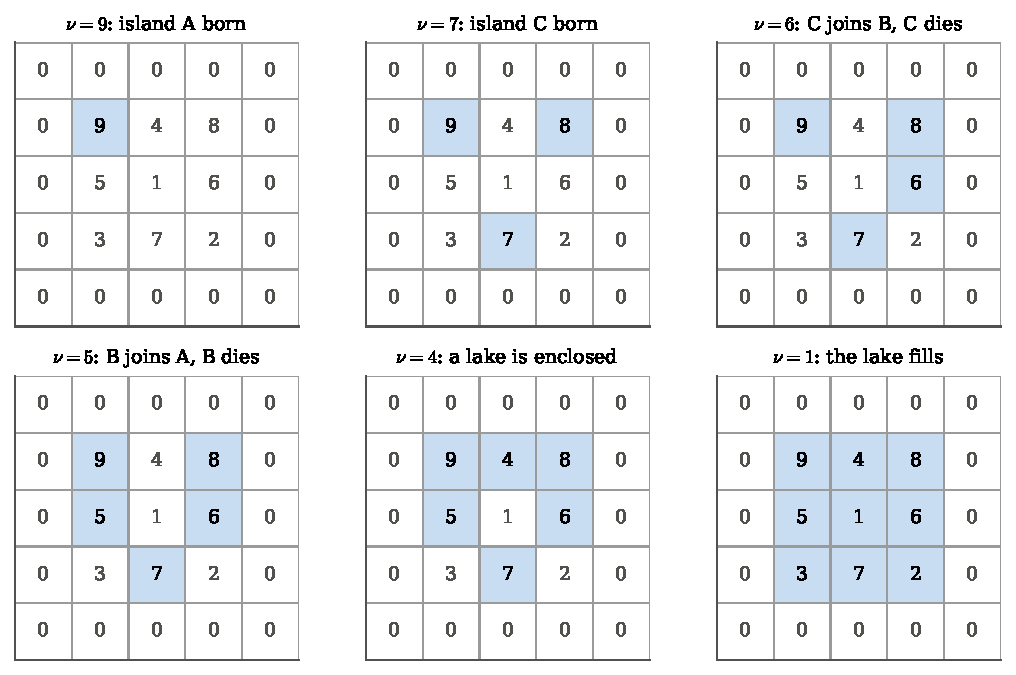
\includegraphics[width=0.86\linewidth]{figures/ch12/b_grid_levels.pdf}
\caption{The $5\times5$ landscape \eqref{12b:eq:grid} at six water levels; dry pixels are shaded. Island A appears
at $9$, B at $8$ (not shown) and C at $7$; C merges into B at $6$ and B into A at $5$. At $4$ the ring of land
around the centre closes and the centre becomes a lake, which drains when the level reaches the centre's height
$1$.}
\label{12b:fig:grid-levels}
\end{figure}

\begin{figure}[htbp]
\centering
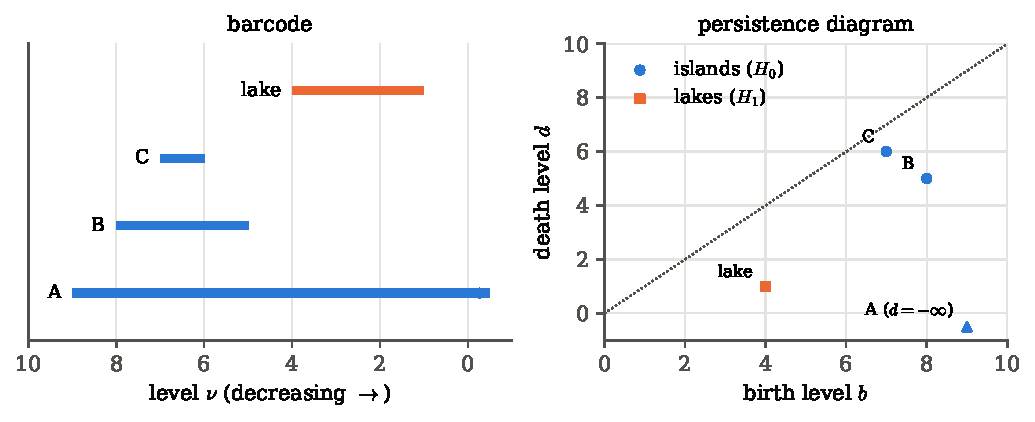
\includegraphics[width=0.86\linewidth]{figures/ch12/b_grid_diagram.pdf}
\caption{The history of \cref{12b:fig:grid-levels} in the two standard forms. Left: the barcode, one bar per
feature, from its birth level to its death level, with the level decreasing to the right. Right: the persistence
diagram, one point $(b,d)$ per feature; the dotted line is $d=b$. Island A, which never dies, is drawn as a
triangle at the bottom of the panel. The farther a point lies below the diagonal, the longer the feature lived.}
\label{12b:fig:grid-diagram}
\end{figure}

\subsection{From the diagram back to the counts}
\label{12b:sec:betti-curve}

The diagram contains every threshold count of \cref{12a:sec:scan}. \emph{How many islands are dry at level
$\nu$?} An island is present at level $\nu$ when it has been born and has not yet died. It is born at $b$ and
the level is decreasing, so it has been born if $\nu\leq b$; it dies at $d$, so it is still alive if $\nu>d$.
Counting the pairs that pass both tests gives the \newterm{Betti curve}
\begin{equation}
  \beta_k(\nu)=\#\{(b,d)\in\mathrm{Dgm}_k:\ d<\nu\leq b\},
  \label{12b:eq:betti-curve}
\end{equation}
where $\mathrm{Dgm}_k$ is the diagram of the $k$-dimensional features. In the diagram plane the condition
$d<\nu\leq b$ picks out the points to the right of the vertical line $b=\nu$ and below the horizontal line
$d=\nu$: a quadrant with its corner on the diagonal at $(\nu,\nu)$ \cite{Pranav2017}.

\paragraph{Example: the line at $\nu=1$.} With the pairs \eqref{12b:eq:line-pairs},
\begin{align*}
  \beta_0(1.0)
  &\eqby{1}\#\{(2.6,-\infty),(2.0,0.5),(1.8,0.9),(1.4,1.1)\ :\ d<1.0\leq b\}\\
  &\eqby{2}\#\{(2.6,-\infty),(2.0,0.5),(1.8,0.9)\}
  = 3 .
\end{align*}
\begin{explain}
  \item Definition \eqref{12b:eq:betti-curve} applied to the four pairs of the line.
  \item All four births are at least $1.0$. The deaths $-\infty$, $0.5$ and $0.9$ are below $1.0$; the death $1.1$
        is not, because C has already merged into D when the water is at $1.0$.
\end{explain}
Directly from \eqref{12b:eq:line}: the heights at least $1.0$ are $h_1=1.8$, $h_3=2.6$ and the run $h_5,h_6,h_7=
1.4,1.1,2.0$, which form three separate intervals. The two counts agree, as they must.

\paragraph{Example: the grid at $\nu=4.5$ and $\nu=3$.} From \eqref{12b:eq:grid-pairs}, at $\nu=4.5$ only the
island pair $(9,-\infty)$ satisfies $d<4.5\leq b$: the pairs $(8,5)$ and $(7,6)$ have deaths $5$ and $6$, not
below $4.5$, so B and C have already merged into A. Hence $\beta_0(4.5)=1$. The lake pair $(4,1)$ fails
$4.5\leq b=4$, so $\beta_1(4.5)=0$: the ring has not closed yet. At $\nu=3$ the lake pair satisfies $1<3\leq4$,
so $\beta_1(3)=1$, and still $\beta_0(3)=1$. The Euler characteristic $\chi=\beta_0-\beta_1$ of
\cref{12a:eq:chi} is $1$ at $\nu=4.5$ and $0$ at $\nu=3$, the values of a disc and of a ring.

\paragraph{Example: the diagram knows more than the curve.} Two different landscapes can have the same Betti curve.
Take one with island pairs $\{(3,1),(2,0)\}$ and another with $\{(3,0),(2,1)\}$, each with one immortal island
besides. In both, $\beta_0$ counts one extra island for $2<\nu\leq3$, two for $1<\nu\leq2$, and one for
$0<\nu\leq1$, so the curves are identical. The diagrams are not. In the first, the island born at $3$ merges
at $1$, and in the second the island born at $3$ survives down to $0$ while the one born at $2$ merges at $1$.
The curve counts how many islands are present at each level; the diagram also says which island is which, so
it knows how long each one lived. That is why research analyses that use Betti curves
\cite{Pranav2017,Wilding2021} also look at the diagrams themselves.

\subsection{Persistence measures robustness to the choice of threshold}
\label{12b:sec:robust}

A feature with pair $(b,d)$ is present in $X_\nu$ for every level in the interval $d<\nu\leq b$, an interval of
width
\begin{equation}
  \Delta\nu=b-d .
  \label{12b:eq:persistence}
\end{equation}
This is the sense in which persistence answers the complaint at the start of the section. Any analysis that
picks one threshold inside that interval sees the feature; any threshold outside it misses it. A feature with
large $\Delta\nu$ is seen by a wide range of reasonable choices, and conclusions drawn from it do not hang on
one of them. A feature with tiny $\Delta\nu$ is seen only in a narrow window of levels, and whether it is
counted at all depends on where the threshold happens to fall. In the diagram, long-lived features are points
far below the diagonal $d=b$, and short-lived ones crowd along it.

\begin{keyidea}[Persistence]
Lowering the threshold through every level turns the excursion sets into a filtration. Each island, lake or
void has a birth level and a death level; the pairs form the persistence diagram, and the number of pairs alive
at any level is the Betti number there \eqref{12b:eq:betti-curve}. The persistence $b-d$ is the range of
thresholds over which a feature exists: points far from the diagonal are structures that no reasonable choice
of threshold can miss.
\end{keyidea}

Whether a short bar is noise or a small real structure is a different question, the question of stability:
if the field is known only up to an error of size $\epsilon$, a feature whose persistence is below about
$2\epsilon$ may have been created by the error, while a feature that persists much longer cannot have been.
\section{Small changes of the field, small changes of the diagram}
\label{12b:sec:stability}

A measured map is never the field itself. It is the field plus instrumental noise, smoothed by a beam, with
the occasional bad pixel. Every wiggle that noise adds to the landscape of \cref{12b:sec:filtration} is a tiny
summit with a tiny pass beside it, so a noisy map has many more islands than the field under it. If each of
them were an equal entry in the persistence diagram, the diagram of the data would have little to do with the
diagram of the physics. What saves the method is that the noise-made islands are not equal entries: they are
born and die at almost the same level, so they sit right next to the diagonal, while the islands of the
underlying field barely move. The statement can be made precise, and checked on simulated maps.

\paragraph{The question.} Suppose every value of the field changes by at most $\epsilon$,
\begin{equation}
  \|f-g\|_\infty\equiv\max_{\bm x}|f(\bm x)-g(\bm x)|\leq\epsilon ,
  \label{12b:eq:supnorm}
\end{equation}
where $f$ is the true field and $g$ the measured one. How far can the persistence diagram of $g$ be from that of
$f$? To answer we need two things: a way to measure the distance between two diagrams, and an argument for
why that distance is small.

\subsection{The simplest case first: a noise wiggle on a slope}
\label{12b:sec:wiggle}

Start where nothing should happen. Let $f$ be a field that only rises along a line, $f(x)\leq f(x')$ whenever
$x<x'$, so its superlevel sets have no features in this stretch: every dry point is joined to the higher
ground on its right. Add noise $\eta(x)$ with $|\eta|\leq\epsilon$, so $g=f+\eta$. Suppose the noise has made a
small summit at $x_p$, a separate island of $g$ born at $g(x_p)$. To merge into the higher ground on its right
it must be joined through the lowest point $x_s>x_p$ between them, the pass, where it dies at $g(x_s)$. How
long can it live?
\begin{align}
  g(x_p)-g(x_s)
  &\eqby{1}\big[f(x_p)-f(x_s)\big]+\big[\eta(x_p)-\eta(x_s)\big]\nonumber\\
  &\relby{2}{\leq} 0+\big[\eta(x_p)-\eta(x_s)\big]\nonumber\\
  &\relby{3}{\leq} \epsilon+\epsilon=2\epsilon .
  \label{12b:eq:wiggle}
\end{align}
\begin{explain}
  \item Write $g=f+\eta$ at both points and regroup.
  \item The pass lies to the right of the summit, $x_s>x_p$, and $f$ rises to the right, so $f(x_p)\leq f(x_s)$.
  \item Each noise value lies between $-\epsilon$ and $\epsilon$, so a difference of two of them is at most
        $2\epsilon$.
\end{explain}
A feature that the noise creates out of nothing has persistence at most $2\epsilon$. Its point $(b,d)$ in the
diagram therefore lies within a vertical (or horizontal) distance $2\epsilon$ of the diagonal, and within
$\epsilon$ of the diagonal point $\big(\tfrac{b+d}2,\tfrac{b+d}2\big)$ in each coordinate. The same chain
read the other way shows that a genuine island of $f$ is not destroyed by the noise unless its own
persistence is below $2\epsilon$, and that its birth (a summit height) and its death (a pass height) each move
by at most $\epsilon$, because every height does.

\subsection{A distance between diagrams}
\label{12b:sec:bottleneck}

To compare two diagrams we pair up their points and ask how far the paired points are. Two complications
appear at once. The diagrams may have different numbers of points, and a short-lived feature present in one may
simply be absent from the other. Both are handled by allowing a point to be paired with the diagonal, which
means ``this feature has shrunk to zero persistence in the other diagram''.

\begin{workdef}[bottleneck distance]
A \newterm{matching} between diagrams $D$ and $D'$ pairs each point of $D$ either with one point of $D'$ or with
the diagonal, and likewise each point of $D'$. The cost of pairing $(b,d)$ with $(b',d')$ is
$\max(|b-b'|,|d-d'|)$ \unpack{the larger of the shift in birth and the shift in death}; the cost of pairing
$(b,d)$ with the diagonal is $(b-d)/2$ \unpack{the shift needed to move it onto the diagonal, to the point
$((b+d)/2,(b+d)/2)$}. The \newterm{bottleneck distance} $d_B(D,D')$ is the smallest possible value of the
largest cost in a matching. \emph{Operationally:} try matchings, record the worst pair in each, and keep the
matching whose worst pair is best.
\end{workdef}

\paragraph{Example: a matching by hand.} Let $D=\{(3,0),\,(2,1.6)\}$ and $D'=\{(2.8,0.1)\}$
(\cref{12b:fig:matching}). Only two matchings are worth trying. In the first, $(3,0)$ goes with $(2.8,0.1)$ and
$(2,1.6)$ goes to the diagonal:
\begin{align*}
  \text{worst cost}
  &\eqby{1}\max\big(\max(|3-2.8|,|0-0.1|),\ \tfrac{2-1.6}{2}\big)
  = \max(0.2,\ 0.2)=0.2 .
\end{align*}
\begin{explain}
  \item The first entry is the cost of the paired points, the second the cost of sending $(2,1.6)$ to the diagonal.
\end{explain}
In the second, $(2,1.6)$ goes with $(2.8,0.1)$ and $(3,0)$ goes to the diagonal: the costs are
$\max(0.8,1.5)=1.5$ and $3/2=1.5$, so the worst is $1.5$. The bottleneck distance is the better of the two,
$d_B=0.2$. In words: the long-lived feature moved by $0.2$, and the short one could have been created or destroyed
by a change of size $0.2$.

\begin{figure}[htbp]
\centering
\begin{tikzpicture}[scale=1.25]
  \draw[faint,->] (-0.2,0) -- (3.9,0) node[lbl,anchor=west] {$b$};
  \draw[faint,->] (0,-0.5) -- (0,3.4) node[lbl,anchor=east] {$d$};
  \draw[faint,dashed] (0,0) -- (3.3,3.3);
  \node[lbl,font=\scriptsize,anchor=south east] at (3.0,3.0) {$d=b$};
  \draw[formblue,thick] (3,0) circle (2.2pt);
  \draw[formblue,thick] (2,1.6) circle (2.2pt);
  \draw[fibreorange,thick] (2.8-0.07,0.1-0.07) rectangle (2.8+0.07,0.1+0.07);
  \draw[thick,black!70] (3,0) -- (2.8,0.1);
  \draw[thick,black!70,dashed] (2,1.6) -- (1.8,1.8);
  \fill[black!70] (1.8,1.8) circle (1.2pt);
  \node[lbl,font=\scriptsize,anchor=north] at (3.0,-0.12) {$(3,0)$};
  \node[lbl,font=\scriptsize,anchor=west] at (2.08,1.52) {$(2,1.6)$};
  \node[lbl,font=\scriptsize,anchor=south] at (2.8,0.2) {$(2.8,0.1)$};
  \node[lbl,font=\scriptsize,anchor=east] at (1.72,1.86) {$(1.8,1.8)$};
\end{tikzpicture}
\caption{The best matching between $D$ (circles) and $D'$ (square). The long-lived point $(3,0)$ is paired with
$(2.8,0.1)$; the short-lived point $(2,1.6)$ has no partner and is sent to the nearest point of the diagonal,
$(1.8,1.8)$, at cost $0.2$. Both costs are $0.2$, so $d_B=0.2$.}
\label{12b:fig:matching}
\end{figure}

\subsection{The stability theorem}
\label{12b:sec:theorem}

The wiggle of \cref{12b:sec:wiggle} gave the bound in the simplest case. Cohen-Steiner, Edelsbrunner and Harer
proved that it holds in general \cite{CohenSteiner2007}.

\begin{keyidea}[Stability of persistence diagrams]
For two fields $f$ and $g$ on the same domain (continuous, with finitely many critical levels, which covers
every pixel map),
\begin{equation*}
  d_B\big(\mathrm{Dgm}_k(f),\,\mathrm{Dgm}_k(g)\big)\leq\|f-g\|_\infty\qquad\text{for every }k.
\end{equation*}
\emph{Physically:} a perturbation of size $\epsilon$ moves every robust feature by at most $\epsilon$ in birth and in
death, and every feature it creates or destroys has persistence at most $2\epsilon$, so it sits within the band
$b-d\leq2\epsilon$ along the diagonal.
\end{keyidea}

\emph{Why it is true, at the physicist's level.} Births and deaths are heights of special points, summits,
passes and lake bottoms, and \eqref{12b:eq:supnorm} says that no height moves by more than $\epsilon$. If the
special points of $g$ were simply the special points of $f$, moved a little, every pair would move by at most
$\epsilon$ in each coordinate and we would be done. The real work in the proof is the case where $g$ has extra
special points (the noise wiggles) or fewer (a feature of $f$ washed out); the slope argument
\eqref{12b:eq:wiggle} shows that such points can only belong to pairs of persistence at most $2\epsilon$, which
the matching sends to the diagonal at cost at most $\epsilon$. The general proof organises this bookkeeping for
all levels at once \cite{CohenSteiner2007}. Note what the theorem does \emph{not} say: it does not bound the number
of new points, only where they can be. A noisy map can have a hundred times more islands than the clean one
and still be within $\epsilon$ of it in the bottleneck distance, because all the extra islands are near the
diagonal \cite{Pranav2017}.

\paragraph{Testing it.} The script \pyname{code/ch12/b03_stability.py} makes a smooth Gaussian field $f$ on a
$128\times128$ grid, adds either white noise or noise smoothed over a pixel and a half, at amplitudes from $0.01$
to $0.4$ standard deviations of $f$, and computes $\|f-g\|_\infty$ and the bottleneck distance between the island
diagrams and between the lake diagrams of $f$ and $g$ (with gudhi's \pyname{bottleneck_distance}, checked once
against persim; they agree to $\PbStabCheck$). Over all $\PbStabTrials$ trials the largest value of
$d_B/\|f-g\|_\infty$ is $\PbStabMaxRatio$: the bound is never broken, and it comes close to being reached
(\cref{12b:fig:stability}, left). It cannot be improved in general, as the simplest perturbation shows: add the same constant
$\epsilon$ to every pixel. Every summit and every pass rises by exactly $\epsilon$, so every point of the diagram moves by
$\epsilon$ in birth and in death, no matching does better, and $d_B=\epsilon=\|f-g\|_\infty$.

\begin{figure}[htbp]
\centering
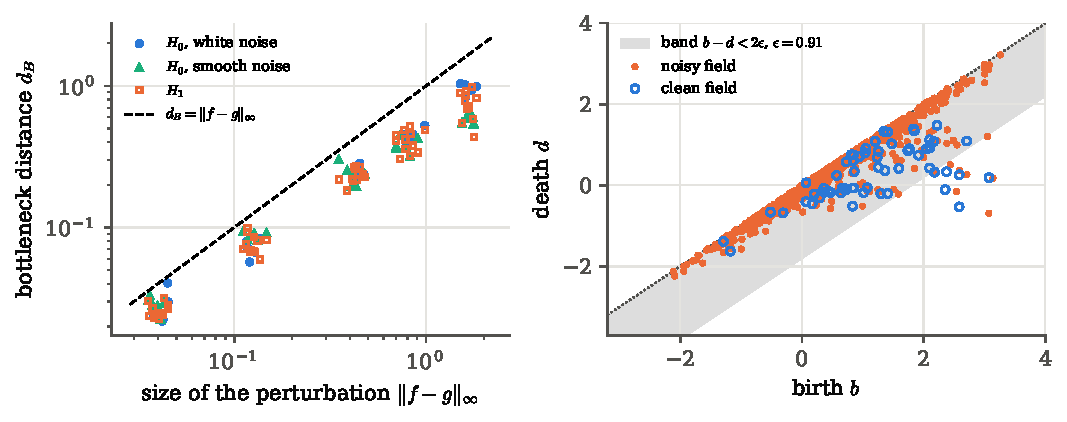
\includegraphics[width=\linewidth]{figures/ch12/b_stability.pdf}
\caption{Left: bottleneck distance between the diagrams of a clean field and a noisy copy, against the size of the
noise, for white and smoothed noise and for islands and lakes. Every point lies below the dashed line
$d_B=\|f-g\|_\infty$. Right: the island diagrams of one clean field (open circles) and of the same field with
white noise of $\PbStabAmp$ standard deviations added (dots). The grey band is $b-d<2\epsilon$. The noise adds a
crowd of points inside the band; the points of the clean field far from the diagonal have partners close by.}
\label{12b:fig:stability}
\end{figure}

\paragraph{Example: where the noise islands sit.} In the right panel of \cref{12b:fig:stability} the white noise
has standard deviation $\PbStabAmp$, but its largest value over the $16\,384$ pixels is $\epsilon=\PbStabEps$ (the
maximum of many Gaussian numbers lies several standard deviations out). The clean field has $\PbStabNclean$
islands; the noisy one has $\PbStabNnoisy$. Of these, $\PbStabNshort$ have persistence below $2\epsilon$, inside the
band the theorem allows for created features. The most persistent island lives for $\PbStabLongClean$ in the clean
field and $\PbStabLongNoisy$ in the noisy one; the tenth most persistent, $\PbStabTenthClean$ and
$\PbStabTenthNoisy$. Smoothing the noisy map over a pixel and a half brings the count back to $\PbStabNsmooth$
islands: the smoothing removes the wiggles that made the short bars, which is the beam of
\cref{8a:sec:beam} doing, for topology, what it does for the power spectrum.

\paragraph{What the bound costs us.} The theorem controls the worst pixel, not the typical one. For Gaussian
noise the worst pixel of a map of $10^4$ to $10^6$ pixels lies about $4$ to $5$ standard deviations out, so the band of $2\epsilon$ is wide,
and many genuine but small features of the field lie inside it, where the theorem cannot tell them from noise.
Worse, one bad pixel (a cosmic-ray hit, an unmasked point source) makes $\epsilon$ large on its own. In practice
we do not rely on the worst-case band. We simulate the noise, pass the simulations through the same pipeline,
and read off where noise features actually fall in the diagram; that is the Monte Carlo of part~12c. The
theorem's job is the qualitative guarantee: features far from the diagonal are safe, and the diagram is a
continuous function of the data, so it is a sensible input to a statistical analysis.

\begin{pitfall}[Bottleneck is not the only distance]
The bottleneck distance looks only at the worst-matched pair and ignores everything else. The
$p$-\newterm{Wasserstein distance} instead adds up the costs, $W_p=\big(\min_{\rm matchings}\sum\text{cost}^p\big)^{1/p}$, so it
feels all the small points near the diagonal too. It is more sensitive to how many noise features there are, and
for that reason it is not bounded by $\|f-g\|_\infty$ alone; its stability needs extra conditions on the fields
\cite{Otter2017}. Use the bottleneck distance when the question is ``did any robust feature move?'', and a
Wasserstein distance when the whole population of features matters.
\end{pitfall}
\section{Computing persistence: union--find and the elder rule}
\label{12b:sec:compute}

The $5\times5$ landscape of \cref{12b:sec:grid} took a page by hand. A $256\times256$ simulated patch has
$65\,536$ pixels, and a HEALPix map at $N_{\rm side}=2048$ has fifty million. The procedure itself does not
change: sort the pixels from the highest to the lowest, let them become dry one at a time, and whenever a new dry
pixel touches dry neighbours, find out which islands those neighbours belong to and merge them, recording a death
by the elder rule. The only hard part is the question ``which island does this pixel belong to?'', asked again
and again. If we answered it by relabelling whole islands at every merger, a big island would be relabelled
thousands of times. The standard answer is a data structure called \newterm{union--find}, which makes each
question cost almost nothing.

\paragraph{The question.} How can a program keep track of which island every dry pixel belongs to, merge two
islands in one step, and remember the summit height of each island, so that it can apply the elder rule?

\subsection{Union--find}
\label{12b:sec:unionfind}

Store each island as a tree of pointers. Every dry pixel $p$ holds one number, $\mathrm{parent}[p]$, the pixel it
points to. Following the pointers from any pixel of an island always ends at the same pixel, the \newterm{root},
which points to itself. The root is the island's name, and we store the island's summit height at the root.
Two operations are needed.
\begin{itemize}[itemsep=1pt,leftmargin=1.2em]
  \item \emph{Find}: to learn which island $p$ belongs to, follow $\mathrm{parent}$ from $p$ until reaching a
        pixel that points to itself.
  \item \emph{Union}: to merge two islands, make the root of one point to the root of the other. One pointer
        changes; nothing else does.
\end{itemize}
Trees made this way can grow long chains, which would make \emph{find} slow. A one-line repair keeps them
shallow: while walking up, make each visited pixel point to its grandparent (\newterm{path halving}). With it, a
long sequence of operations costs, on average, a small constant number of steps each, so the total work is
proportional to the number of pixels, apart from the sort that puts them in order of height
\cite{Otter2017}.

\begin{figure}[htbp]
\centering
\begin{tikzpicture}[
  px/.style={circle,draw=formblue,thick,minimum size=6.5mm,inner sep=0pt,font=\scriptsize},
  rt/.style={px,fill=formblue!15},
  ptr/.style={->,thick,black!60}]
  \begin{scope}
    \node[rt] (a9) at (0,1.6) {9};
    \node[rt] (b8) at (2.4,1.6) {8};
    \node[px] (b6) at (1.9,0.5) {6};
    \node[px] (b7) at (2.9,0.5) {7};
    \draw[ptr] (b6) -- (b8);
    \draw[ptr] (b7) -- (b8);
    \node[lbl,font=\scriptsize,align=center] at (1.2,-0.5) {just before the pixel of height 5:\\ two islands, roots 9 and 8};
  \end{scope}
  \begin{scope}[xshift=6.2cm]
    \node[rt] (A9) at (0.6,2.2) {9};
    \node[px] (A5) at (0.6,1.1) {5};
    \node[px] (B8) at (1.8,1.1) {8};
    \node[px] (B6) at (1.3,0.0) {6};
    \node[px] (B7) at (2.3,0.0) {7};
    \draw[ptr] (A5) -- (A9);
    \draw[ptr,bdryred] (B8) -- (A9);
    \draw[ptr] (B6) -- (B8);
    \draw[ptr] (B7) -- (B8);
    \node[lbl,font=\scriptsize,align=center] at (0.9,-0.8) {one island, root 9;\\ the pair $(8,5)$ is recorded};
  \end{scope}
\end{tikzpicture}
\caption{Union--find on the island step of the $5\times5$ example at level $5$ (\cref{12b:sec:grid}). Each circle
is a dry pixel labelled by its height, each arrow its parent pointer; the shaded circles are roots, which carry the
summit height of their island. When the pixel of height $5$ joins both islands, the root of the younger island
(summit $8$) is made to point to the root of the older one (summit $9$, red arrow), and the death of the younger
island at level $5$ is written down.}
\label{12b:fig:unionfind}
\end{figure}

The whole algorithm for the islands of a pixel map is then the function \pyname{islands} of
\pyname{code/ch12/lib_persist.py}:

\pyfile[firstline=30,lastline=62,firstnumber=30]{code/ch12/lib_persist.py}{Islands ($H_0$) of the superlevel sets by union--find}

\noindent Line 34 sorts the pixels from the highest to the lowest: this is the falling water. Lines 35--36 hold
the two arrays of union--find, \pyname{parent} (with $-1$ for a pixel still under water) and \pyname{peak}, the
summit height stored at each root. Lines 39--43 are \emph{find} with path halving. The loop of line 46 makes one
pixel dry per step. Line 47 makes it a one-pixel island, its own root, with its own height as summit. Lines
49--52 visit the eight neighbours and skip those off the map or still wet. Line 53 finds the roots of the new
pixel and of the neighbour. If they differ, the two islands are merging at the level $h[p]$ of the new pixel. Lines
56--57 apply the elder rule: \pyname{r1} becomes the root with the higher summit. Lines 58--59 record the death of
the younger island, $(\text{its summit},\ h[p])$, unless the younger ``island'' is just the new pixel itself, whose
summit equals $h[p]$ and whose pair would have zero persistence. Line 60 is the \emph{union}. When every pixel is
dry, line 61 adds the island that never dies.

\paragraph{Example: the code on the hand example.} Run on the grid \eqref{12b:eq:grid}, \pyname{islands} returns the
pairs $(7,6)$, $(8,5)$ and $(9,-\infty)$, exactly \eqref{12b:eq:grid-pairs}, in the order in which the deaths happen
(\pyname{code/ch12/b01_hand_examples.py}). gudhi, given the same grid, returns the same three pairs.

\subsection{Lakes from islands: duality in the plane}
\label{12b:sec:lakes}

Lakes need a second idea. A lake of the dry land is a body of water that does not reach the open sea. So instead
of watching the land, watch the water. The water at level $\nu$ is the set $\{\phi<\nu\}$. As the level falls, the
water shrinks; read backwards, with the level rising, the water grows, starting at the lowest points of the map and
spreading. That is exactly the island story for the upside-down landscape $-\phi$: its summits are the lake bottoms
of $\phi$, and its passes are the passes of $\phi$.

\emph{The translation.} Run \pyname{islands} on $-\phi$, with two changes. First, water pixels are connected only
through edges, 4-neighbours, because the land is 8-connected and the two must be dual (\cref{12a:sec:pixels}).
Second, surround the map with a frame of open sea that is always wet, by giving the frame the height $+\infty$ in
$-\phi$; the frame then becomes the oldest island of $-\phi$, and any water connected to the edge of the map merges
into it. Now take a water body of $-\phi$ born at $-\phi=-m$ and merging at $-\phi=-s$. In the language of the land:
the water body has its bottom at height $m$ and joins other water through a pass of height $s>m$. With the level
falling, it is part of a larger body while $\nu>s$; when $\nu$ drops below $s$ it is cut off from the rest, so if
the rest is the sea, a lake is born at $s$; and it drains when $\nu$ drops below its bottom $m$. So a pair
$(-m,-s)$ of $-\phi$ becomes the lake pair $(s,m)$ of $\phi$. On the hand example the centre pixel is a water
island of $-\phi$ born at $-1$. In the reversed picture the water rises; the first of its four edge-neighbours to
go under is the pixel of height $4$, which is already joined to the border, so the centre's water body merges into
the sea at $-4$. The lake pair is $(4,1)$, as found by hand. That this bookkeeping gives exactly the
lakes, the holes of the land, is a case of \newterm{Alexander duality} (see the topology notes): in the plane, the
holes of a set are the bounded pieces of its complement.

\pyfile[firstline=65,lastline=77,firstnumber=65]{code/ch12/lib_persist.py}{Lakes ($H_1$) by duality: the islands of $-\phi$ with a sea around the map}

\noindent Line 74 builds $-\phi$ with the frame of sea, line 75 runs the island code with 4-neighbours, line 76
drops the one immortal water body (the sea), and line 77 translates each pair back.

\emph{On the torus the shortcut fails.} A periodic map, such as a simulation box, has no edge and so no open sea.
Two new things happen. A band of land that wraps around the torus contains a loop that encloses no lake; and the
water can also wrap around, so no water body is ``outside''. The lake count then misses the loops that wind around
the torus, and the frame of sea, if we add it, cuts features that should continue across the edges. For periodic
maps we therefore use gudhi's \pyname{PeriodicCubicalComplex} (\cref{12b:sec:web}), which builds the torus
directly.

\subsection{Checks against the libraries, and timing}
\label{12b:sec:checks}

\pyname{code/ch12/b02_grf_persistence.py} makes one Gaussian field on a $\PbGrfN\times\PbGrfN$ grid, smoothed on
$\PbGrfR$ pixels (the recipe of \cref{7a:sec:simulate}), and runs four independent checks.
\begin{itemize}[itemsep=1pt,leftmargin=1.2em]
  \item \emph{gudhi.} Its \pyname{CubicalComplex}, built from the pixels as squares, computes the persistence of
        the sublevel sets of $-\phi$, which are our superlevel sets of $\phi$ with the same 8- and
        4-neighbour rules. Both codes find $\PbGrfNzero$ island pairs and $\PbGrfNone$ lake pairs, and the
        bottleneck distance between our diagrams and gudhi's (computed by persim) is $\PbGrfdBgudhi$: they are
        identical.
  \item \emph{ripser.} Its \pyname{lower_star_img} computes the island pairs of an image. The bottleneck distance
        to ours is $\PbGrfdBripser$, the rounding error of the single-precision numbers ripser uses internally.
  \item \emph{scipy.} At 61 levels from $-3$ to $3$ we count the islands directly with
        \pyname{scipy.ndimage.label} (8-neighbours) and the lakes as the 4-connected water bodies that do not
        touch the edge. These counts and the Betti curves \eqref{12b:eq:betti-curve} read from our diagrams differ
        by at most $\PbGrfMismatch$ at any level.
  \item \emph{scikit-image.} \pyname{skimage.measure.label} (with \pyname{connectivity=2}, its name for 8-neighbours)
        counts the islands again, and \pyname{skimage.measure.euler_number} computes $\chi$ of the dry land by counting
        cells, as in \cref{12a:sec:vef}. They equal $\beta_0$ and $\beta_0-\beta_1$ from our diagrams at
        every level.
\end{itemize}
A fifth check is a physical one. The field $e^{0.8\phi}$ is a strictly increasing function of $\phi$, so by the
argument of \cref{12a:sec:monotone} its dry land at level $e^{0.8\nu}$ is the dry land of $\phi$ at level $\nu$.
Its diagram must be the diagram of $\phi$ with every level relabelled, and it is: taking the logarithm of its
pairs and dividing by $0.8$ gives back the pairs of $\phi$ exactly.

\begin{figure}[htbp]
\centering
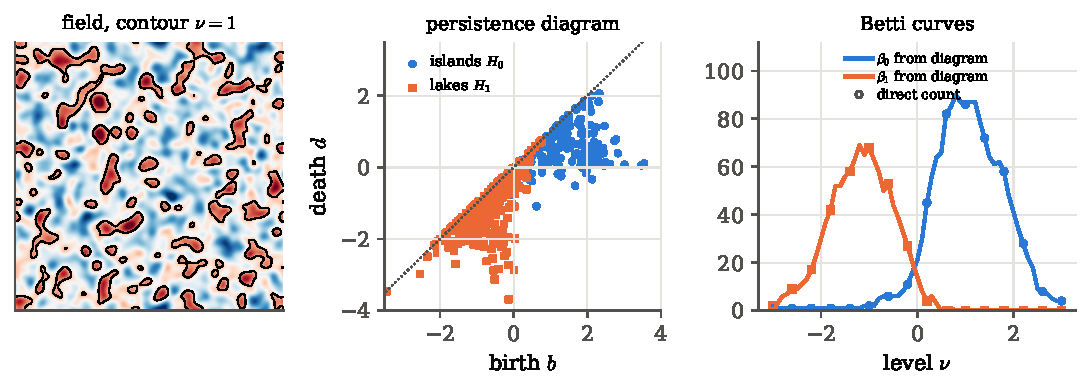
\includegraphics[width=\linewidth]{figures/ch12/b_grf_diagram.pdf}
\caption{One $256\times256$ Gaussian field and its persistence. Left: the field, with the boundary of the dry land
at $\nu=1$. Middle: the diagrams of islands (circles) and lakes (squares). Islands are born at positive levels,
the summits, and lakes die at negative levels, the lake bottoms. Right: the Betti curves read from the diagrams
(lines) and counted directly with \pyname{scipy.ndimage.label} (open symbols).}
\label{12b:fig:grf-diagram}
\end{figure}

\Cref{12b:fig:grf-diagram} shows what the diagram of a smooth random field looks like. The islands are born at
summits, almost all above $\nu=0$, and die at passes, spread from about $-2$ to $2$. The lakes are their mirror
image: born at passes, dying at lake bottoms, almost all below $0$. The mirror symmetry is the one of
\cref{12a:sec:scan}: a Gaussian field is as likely as its negative, so the lakes of $\phi$ are statistically the
islands of $-\phi$. The longest-lived island lives for $\PbGrfMaxPers$, and a fraction $\PbGrfShortFrac$ of the
islands live for less than $0.25$; even without noise, a smooth field has many shallow summits sitting on the
shoulders of bigger ones.

\paragraph{Timing.} The union--find code is plain Python, one loop over pixels. Its run time grows in proportion to
the number of pixels (a fitted power of $\PbTimeSlope$), from about a second at $256^2$ to
$\PbTimeOursBig$\,s for islands and lakes at $1024^2$; gudhi, written in C++, takes $\PbTimeGudhiBig$\,s there
(\cref{12b:fig:timing}). Both are fast enough for every map used in this chapter's experiments. Scaled to a full-resolution \textit{Planck} map of fifty
million pixels, the measured times become about thirteen minutes for the Python code and about a minute and a half for gudhi (on
the sphere the neighbours would come from \pyname{healpy.get_all_neighbours} instead of the grid).

\begin{figure}[htbp]
\centering
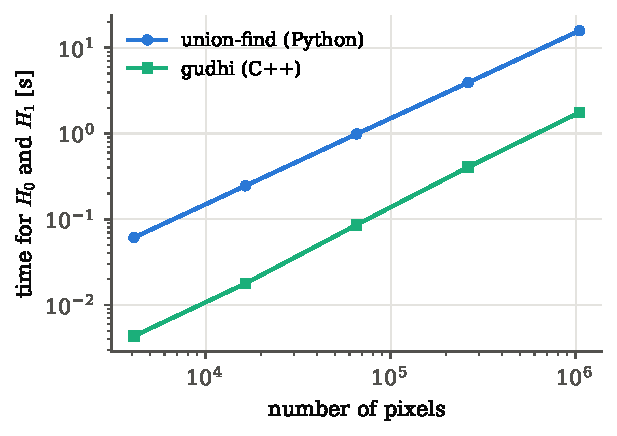
\includegraphics[width=0.55\linewidth]{figures/ch12/b_timing.pdf}
\caption{Time to compute the island and lake diagrams against the number of pixels, for the union--find code of
\cref{12b:sec:unionfind} and for gudhi. Both grow in proportion to the number of pixels; the compiled library is about ten
times faster.}
\label{12b:fig:timing}
\end{figure}

\begin{inpractice}[Persistence software in research]
Research codes never write their own union--find. For pixel maps and simulation boxes the standard tools are
gudhi's cubical complexes (periodic or not), Cubical Ripser, and DIPHA for maps too large for one machine; for point
clouds, ripser and gudhi's Rips and alpha complexes; and for diagrams, persim and gudhi's own distances
\cite{Otter2017}. Cosmic-web studies compute persistence on a Delaunay tessellation of the particles with the
density estimated at each particle, using the PHAT library \cite{Pranav2017,Wilding2021}. The from-scratch code
earns its place as a check: on a small map, a disagreement between it and the library almost always means a
convention has been mixed up (superlevel against sublevel sets, 4- against 8-neighbours, the sign of the field).
\end{inpractice}
\section{Point clouds: shapes grown from points}
\label{12b:sec:points}

A galaxy survey or an $N$-body simulation does not hand us a field. It hands us points: positions of galaxies,
haloes or dark-matter particles. One way forward is to turn the points into a density field on a grid and use
the landscape of the previous sections; \cref{12b:sec:web} does that. The other is to build shapes directly from
the points. Put a small ball around every point and let all the balls grow together. When two balls touch, their
points are linked; when three points are pairwise linked, the triangle between them is filled in. At a small
radius every point is alone. As the radius grows, close points join into clusters, clusters join each other, rings
of points close into loops, and the loops eventually fill in. The radius plays the role the water level played
for a field, and the same bookkeeping of births and deaths applies.

\paragraph{The question.} For a set of points, at which linking distance does each cluster stop being separate,
and at which distances do loops of points appear and fill in? And how do we compute this without drawing balls?

\begin{workdef}[Vietoris--Rips filtration]
For points $\bm x_1,\dots,\bm x_n$ and a scale $r\geq0$, the \newterm{Vietoris--Rips complex} $\mathrm{VR}_r$
contains every point, an edge between $\bm x_i$ and $\bm x_j$ whenever $|\bm x_i-\bm x_j|\leq r$, and a filled
triangle (and higher simplices) on every set of points that are pairwise within $r$ \unpack{a triangle enters
exactly when its longest edge does}. As $r$ grows the complex only gains edges and triangles, so it is a
filtration. Every point is born at $r=0$; a cluster dies at the $r$ where it joins another; a loop is born at the
length of the edge that closes it and dies at the length of the edge that completes the triangles filling it.
\end{workdef}

In this filtration the parameter increases, so births come before deaths, $b\leq d$, and the diagram points lie
above the diagonal; this is the convention of every point-cloud library. \Cref{12b:fig:rips} shows the complex of
a noisy ring of $\PbCloudNc$ points with a small clump of $\PbCloudNk$ beside it at three scales.

\begin{figure}[htbp]
\centering
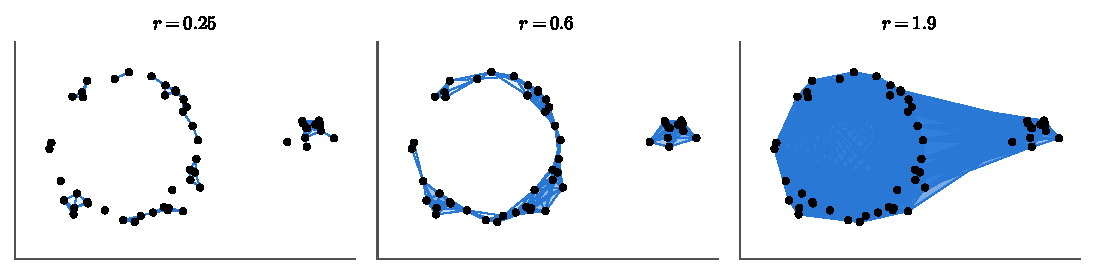
\includegraphics[width=\linewidth]{figures/ch12/b_rips.pdf}
\caption{The Vietoris--Rips complex of a noisy ring with a clump beside it, at three scales $r$. At $r=0.25$ only
near neighbours are linked. At $r=0.6$ the ring is linked all the way round except for one gap on its left, which
closes a little later into a loop around an empty middle, and the clump is one cluster. At $r=1.9$ triangles have filled the middle of the ring and the clump is joined to it: one blob.}
\label{12b:fig:rips}
\end{figure}

\subsection{Clusters: the minimum spanning tree}
\label{12b:sec:mst}

Connectivity in $\mathrm{VR}_r$ is decided by the edges alone: triangles fill area but join nothing that their
edges have not already joined. So to follow the clusters we only need to add the edges in order of length and
ask, for each edge, whether it joins two different clusters. That is \newterm{Kruskal's algorithm}: sort all
$n(n-1)/2$ edges by length; take them one by one; if an edge joins two different clusters, merge them (one dies
at that length) and keep the edge; if it joins a cluster to itself, skip it. The kept edges form the
\newterm{minimum spanning tree}, the shortest network of edges that connects all the points, and their lengths are
exactly the deaths of the island diagram of the points. All births are at $0$, so the elder rule never has to
choose by age; any choice of which cluster dies gives the same pairs.

\paragraph{Example: six points by hand.} Take $A=(0,0)$, $B=(1,0)$, $C=(0,1)$, $D=(4,0)$, $E=(5,0)$, $F=(4,2)$
(\cref{12b:fig:six}). The shortest distances, in order, are $AB=AC=DE=1$, $BC=\sqrt2$, $DF=2$, $EF=\sqrt5$, then
$BD=3$. Kruskal takes $AB$ (one cluster dies at $1$), $AC$ (another at $1$), $DE$ (another at $1$). $BC$ joins $B$
and $C$, already in one cluster through $A$, so it is skipped; at the same length the triangle $ABC$ enters (its
longest edge is $BC$), so no loop ever exists there. $DF$ joins $F$ to the cluster $\{D,E\}$: a death at $2$. $EF$ is
skipped. $BD=3$ joins the two clusters: a death at $3$. The island diagram is
\begin{equation}
  \{(0,1),\ (0,1),\ (0,1),\ (0,2),\ (0,3),\ (0,\infty)\},
  \label{12b:eq:six}
\end{equation}
and the minimum spanning tree has total length $1+1+1+2+3=8$. Read the bars: three die at $1$, the spacing inside
the two groups; one at $2$, the loose point $F$; and one bar, from $0$ to $3$, stands out. It says that there are two
groups of points, separate for all scales between $2$ (when the second group is complete) and $3$ (when they join).
The script \pyname{b04_point_cloud.py} returns exactly these deaths, and so does ripser.

\begin{figure}[htbp]
\centering
\begin{tikzpicture}[scale=0.95]
  \foreach \n/\x/\y/\a in {A/0/0/north east,B/1/0/north west,C/0/1/east,D/4/0/north,E/5/0/north west,F/4/2/east}{
    \fill (\x,\y) circle (2pt);
    \node[lbl,anchor=\a] at (\x,\y) {$\n$};
  }
  \draw[form] (0,0) -- (1,0);
  \draw[form] (0,0) -- (0,1);
  \draw[form] (4,0) -- (5,0);
  \draw[form] (4,0) -- (4,2);
  \draw[bdry] (1,0) -- (4,0);
  \draw[faint,dashed] (1,0) -- (0,1);
  \draw[faint,dashed] (5,0) -- (4,2);
  \node[lbl,font=\scriptsize,anchor=north] at (0.5,-0.05) {$1$};
  \node[lbl,font=\scriptsize,anchor=east] at (-0.05,0.5) {$1$};
  \node[lbl,font=\scriptsize,anchor=south] at (4.5,0.02) {$1$};
  \node[lbl,font=\scriptsize,anchor=east] at (3.95,1.0) {$2$};
  \node[lbl,font=\scriptsize,anchor=south] at (2.5,0.02) {$3$};
\end{tikzpicture}
\caption{The six points of the hand example and their minimum spanning tree. Blue edges join points within a group;
the red edge, of length $3$, is the last one added and joins the two groups. Dashed edges are skipped by Kruskal's
algorithm because their endpoints are already connected.}
\label{12b:fig:six}
\end{figure}

\emph{Two old friends.} Hierarchical clustering with ``single linkage'' joins at each step the two clusters with the
closest pair of members; its merge heights are the edge lengths of the minimum spanning tree, and
\pyname{scipy.cluster.hierarchy.linkage(X, method="single")} returns exactly our deaths. And the friends-of-friends
group finder used on $N$-body simulations, which links any two particles closer than a linking length $b$ and calls
each connected group a halo, returns the clusters of $\mathrm{VR}_b$. The island diagram of the particles therefore
contains the friends-of-friends catalogue for every linking length at once: the number of haloes at linking length
$b$ is the number of bars still alive at $r=b$.

\pyfile[firstline=98,lastline=123,firstnumber=98]{code/ch12/lib_persist.py}{Island diagram of a point cloud: Kruskal's minimum spanning tree}

\noindent Lines 105--106 list every pair of points and its distance. The loop of line 116 takes the edges from the
shortest up; \pyname{root} is the \emph{find} of \cref{12b:sec:unionfind}. Lines 117--120 keep an edge only when it
joins two different clusters, and record its length as a death. After $n-1$ deaths a single cluster is left and the
loop can stop.

\subsection{Loops: reducing the boundary matrix}
\label{12b:sec:reduction}

Loops cannot be found with union--find, which only knows who is connected to whom. The general algorithm keeps,
for every edge and triangle, the list of its faces, and does linear algebra on these lists
\cite{Edelsbrunner2002,Pranav2017}.

\paragraph{Example: the unit square by hand.} Four points at the corners of a unit square, $v_0=(0,0)$,
$v_1=(1,0)$, $v_2=(1,1)$, $v_3=(0,1)$. At $r=1$ the four sides enter. Every triangle on these points needs a
diagonal, of length $\sqrt2$, so no triangle enters yet: the four sides enclose an empty loop, and a loop is born at
$r=1$. At $r=\sqrt2$ both diagonals enter and with them all four triangles, which cover the square: the loop dies.
The loop diagram is $\{(1,\sqrt2)\}$.

\emph{How the algorithm finds this.} List the cells in the order they enter: the four points, then the sides
$e_{01},e_{12},e_{23},e_{03}$ (length $1$), then the diagonals $e_{02},e_{13}$ and the triangles (length $\sqrt2$).
Write each cell as the list of its faces, its \newterm{boundary}: $\partial e_{01}=\{v_0,v_1\}$,
$\partial t_{023}=\{e_{02},e_{23},e_{03}\}$, and so on. Lists are added modulo $2$: a face present in both lists
cancels. Go through the cells in order. For each, look at the latest-entering face in its list, its
\emph{lowest} entry. If an earlier cell already owns that lowest entry, add that cell's (already reduced) list to
this one and look again. Stop when the lowest entry is new, or the list is empty.
\begin{itemize}[itemsep=1pt,leftmargin=1.2em]
  \item $e_{01}$: list $\{v_0,v_1\}$, lowest $v_1$, new. So $e_{01}$ kills the cluster born at $v_1$: the pair $(0,1)$.
        Likewise $e_{12}$ kills $v_2$ and $e_{23}$ kills $v_3$.
  \item $e_{03}$: list $\{v_0,v_3\}$. Lowest $v_3$ is owned by $e_{23}$: add, $\{v_0,v_3\}+\{v_2,v_3\}=\{v_0,v_2\}$.
        Lowest $v_2$ is owned by $e_{12}$: add, giving $\{v_0,v_1\}$; lowest $v_1$ is owned by $e_{01}$: add, giving
        $\{\}$. The list is empty: $e_{03}$ kills nothing, so it creates something. It is the edge that closes the
        loop, born at $r=1$.
  \item The diagonals reduce to empty lists the same way: each closes a new loop at $\sqrt2$.
  \item The triangle $t_{012}$, list $\{e_{01},e_{12},e_{02}\}$, lowest $e_{02}$, new: it kills the loop that $e_{02}$
        created, the pair $(\sqrt2,\sqrt2)$, of zero persistence. The triangle $t_{013}$ kills the loop of $e_{13}$ the
        same way.
  \item The triangle $t_{023}$, list $\{e_{02},e_{23},e_{03}\}$. Lowest $e_{02}$ is owned by $t_{012}$: add, giving
        $\{e_{01},e_{12},e_{23},e_{03}\}$, the four sides. Lowest $e_{03}$, new: $t_{023}$ kills the loop born when
        $e_{03}$ entered, the pair $(1,\sqrt2)$.
\end{itemize}
The reduced list of $t_{023}$ is the boundary of the square: the algorithm has discovered that the two triangles
$t_{012}$ and $t_{023}$ together fill the loop of the four sides. Every pair of a persistence diagram, in any
dimension, is found this way \cite{Edelsbrunner2002}.

\pyfile[firstline=126,lastline=159,firstnumber=126]{code/ch12/lib_persist.py}{Persistence of a Rips filtration by reducing the boundary matrix (small clouds)}

\noindent Lines 133--138 build all points, edges and triangles with their entry scale, the longest edge. Line 139
sorts them, faces before the cells they bound at equal scale. In the loop of line 144, line 145 builds the list of
faces, lines 146--147 do the additions, and lines 148--154 record a pair when the reduced list is not empty (pairs of
zero persistence are dropped). Lines 155--158 add the features that are never killed.

\paragraph{Example: a ring and a clump.} For the $\PbCloudN$ points of \cref{12b:fig:rips}, the loop diagram has one
point far from the diagonal, $(\PbLoopBirth,\,\PbLoopDeath)$: the ring closes at $r\approx\PbLoopBirth$, about the
largest gap between neighbouring points on it, and fills at $r\approx\PbLoopDeath$, when triangles can span its
middle; the next loop lives for only $\PbLoopSecond$. In the island diagram, the longest finite bar ends at
$\PbGapEdge$, the distance at which the clump joins the ring (\cref{12b:fig:cloud-diagram}). Our reduction, ripser and
gudhi's \pyname{RipsComplex} give the same loop diagram: the bottleneck distances between them are $\PbdBbrute$ and
$\PbdBgudhi$, single-precision rounding again. Our Kruskal deaths equal ripser's island deaths and scipy's
single-linkage heights to machine precision.

\begin{figure}[htbp]
\centering
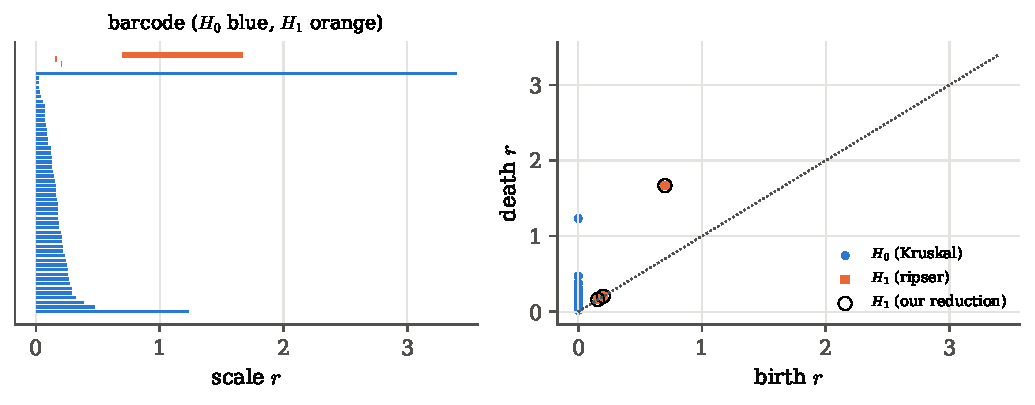
\includegraphics[width=0.92\linewidth]{figures/ch12/b_cloud_diagram.pdf}
\caption{Persistence of the ring and clump of \cref{12b:fig:rips}. Left: the barcode; every island bar starts at $r=0$,
and the one long loop bar (orange, top) is the ring. Right: the diagram, with island points on the vertical axis
(birth $0$) and loop points above the diagonal; the ring's loop, found identically by ripser and by our
reduction (open circles), stands far from the diagonal.}
\label{12b:fig:cloud-diagram}
\end{figure}

\paragraph{Cost.} The reduction works on every triangle, and there are $n(n-1)(n-2)/6$ of them: already
$\PbSimplices$ cells for $\PbCloudN$ points, and our pure-Python reduction takes $\PbTimeBrute$\,s on them. It is a
teaching code. ripser avoids building most of the triangles and reduces cleverly, and handles $\PbCloudBig$ points
(islands and loops) in $\PbTimeRipserBig$\,s; Kruskal alone, for islands only, takes $\PbTimeKruskalBig$\,s there.
For millions of galaxies in three dimensions, research codes replace the Rips complex by the much smaller alpha
complex built on the Delaunay tessellation, which gives the same shapes as growing balls without the explosion of
cells \cite{Otter2017,Pranav2017}.
\section{The cosmic web: clusters, tunnels and voids}
\label{12b:sec:web}

The matter of the late universe is arranged in a web: dense clusters at the nodes, filaments joining them, thin
walls between filaments, and large nearly empty voids (see \cref{ch:T1} for the objects and the cosmology notes for
their physics). The same three-dimensional density contrast $\delta(\bm x)$ has already been met twice. In
\cref{T3a:sec:web} we measured the genus of its excursion sets in simulated Gaussian boxes and found it equal to the
Gaussian formula \cref{T3a:eq:genus3d}: a Gaussian field is a sponge at the median density. In \cref{12a:sec:gkf3}
the expected Euler characteristic of a three-dimensional Gaussian field was derived from its critical points. Both
results are about one number per threshold, the alternating sum $\chi=\beta_0-\beta_1+\beta_2$. What is new here is
to split that sum into its three counts and to follow each feature through the thresholds, as Pranav and
collaborators proposed for the cosmic web \cite{Pranav2017} and Wilding and collaborators carried out for $\Lambda$CDM
simulations \cite{Wilding2021}.

In three dimensions the dry land $X_\nu=\{\delta\geq\nu\}$ (with $\delta$ in units of its standard deviation) has
three kinds of features. $\beta_0$ counts its separate pieces: \emph{clusters}. $\beta_1$ counts independent
\emph{tunnels}: loops in the land around which a string could be threaded, the holes of a doughnut, formed for example
by a ring of filaments around an empty channel. $\beta_2$ counts \emph{voids}: pockets of low density completely sealed
inside the land, like the hollow of a ball. A sum with signs can hide its terms; two clusters and one hollow ball have
the same $\chi=2$ (\cref{T3a:fig:betti}). The separate counts cannot hide them.

\paragraph{Example: three solids.} A solid ball has one piece, no tunnel and no sealed pocket: $(\beta_0,\beta_1,\beta_2)=
(1,0,0)$, $\chi=1$. A solid doughnut has one piece and one tunnel, through its hole: $(1,1,0)$, $\chi=0$. A hollow ball, a
thick shell around an empty pocket, has one piece and one void: $(1,0,1)$, $\chi=2$. A pretzel with two holes has
$(1,2,0)$ and $\chi=-1$. In each case $\chi=\beta_0-\beta_1+\beta_2$, and only the separate counts say whether a
negative $\chi$ comes from tunnels or a positive one from clusters rather than voids.

\paragraph{The question.} As the density threshold is lowered through a Gaussian random field in three dimensions, at
which levels are clusters, tunnels and voids most numerous, and do the three Betti curves, combined with their signs,
reproduce the Euler characteristic predicted for a Gaussian field?

\subsection{Which events create and destroy which features}
\label{12b:sec:events}

\Cref{12a:sec:morse} showed that the topology of the dry land changes only when the level passes the height of a
critical point, a point where the gradient of the field vanishes, and that the type of the point fixes the type of
change. In three dimensions there are four types, told apart by how many of the three principal curvatures of the
field are negative (how many directions the field falls away in). Take them in the order in which the falling level
meets them.
\begin{itemize}[itemsep=1pt,leftmargin=1.2em]
  \item A \emph{maximum} (the field falls in all three directions) is the top of a cluster. Passing it creates a new
        cluster: $\beta_0$ increases by one.
  \item A \emph{filament saddle} (falls in two directions, rises in one) is the lowest point along the spine of a
        filament between two higher regions. Passing it adds a bridge of land. If the bridge joins two clusters, one of
        them dies ($\beta_0$ decreases); if it joins a cluster to itself, it closes a ring, and a tunnel is born
        ($\beta_1$ increases).
  \item A \emph{wall saddle} (falls in one direction, rises in two) is the lowest point of a thin sheet stretched
        across an opening. Passing it adds a membrane of land. If the membrane spans a ring, the tunnel is closed off
        and dies ($\beta_1$ decreases); if it closes the last opening of a pocket, a void is sealed and born ($\beta_2$
        increases).
  \item A \emph{minimum} (the field rises in all directions) is the bottom of a void. Passing it fills the void
        ($\beta_2$ decreases).
\end{itemize}
\Cref{12b:fig:events} summarises the list. It explains the order in which the three Betti curves rise and fall:
clusters are born at maxima, which are mostly high; tunnels at filament saddles, typical of intermediate levels;
voids at wall saddles and they die at minima, mostly low. For a Gaussian field, which is as likely as its negative,
the list is symmetric: the voids of $\delta$ are the clusters of $-\delta$, so $\beta_2$ at level $\nu$ should
behave on average like $\beta_0$ at $-\nu$, and $\beta_1$ should be symmetric about $\nu=0$.

\begin{figure}[htbp]
\centering
\begin{tikzpicture}[
  ev/.style={draw=black!45,rounded corners=2pt,align=center,font=\small,minimum width=2.6cm,minimum height=1.0cm,
             fill=formblue!6},
  arr/.style={->,thick,black!55}]
  \node[ev] (mx) at (0,0) {maximum\\ \scriptsize falls in 3 directions};
  \node[ev] (fs) at (3.6,0) {filament saddle\\ \scriptsize falls in 2};
  \node[ev] (ws) at (7.2,0) {wall saddle\\ \scriptsize falls in 1};
  \node[ev] (mn) at (10.8,0) {minimum\\ \scriptsize falls in 0};
  \draw[arr] (mx) -- (fs);
  \draw[arr] (fs) -- (ws);
  \draw[arr] (ws) -- (mn);
  \node[font=\scriptsize,align=center,anchor=north] at (0,-0.75) {$\beta_0+1$\\ cluster born};
  \node[font=\scriptsize,align=center,anchor=north] at (3.6,-0.75) {$\beta_0-1$ (clusters merge)\\ or $\beta_1+1$ (tunnel born)};
  \node[font=\scriptsize,align=center,anchor=north] at (7.2,-0.75) {$\beta_1-1$ (tunnel closed)\\ or $\beta_2+1$ (void sealed)};
  \node[font=\scriptsize,align=center,anchor=north] at (10.8,-0.75) {$\beta_2-1$\\ void filled};
  \node[font=\scriptsize,anchor=south] at (5.4,0.6) {order in which the falling level typically meets them};
\end{tikzpicture}
\caption{The four kinds of critical point of a three-dimensional field and what passing each does to the dry land
$\{\delta\geq\nu\}$ as the level falls. Every birth or death in the three persistence diagrams happens at one of them.}
\label{12b:fig:events}
\end{figure}

\subsection{Betti curves of Gaussian boxes}
\label{12b:sec:grf3d}

\pyname{code/ch12/b05_cosmic_web.py} draws $\PbWebBoxes$ periodic Gaussian boxes of $\PbWebN^3$ cells with a power
spectrum $P(k)\propto k^{-1.5}e^{-k^2R^2}$, $R=\PbWebR$ cells (the simulator of \cref{7a:sec:simulate} in three
dimensions), and computes the persistence of the superlevel sets on the 3-torus with gudhi's
\pyname{PeriodicCubicalComplex}. The Betti curves are then counted from the diagrams with \eqref{12b:eq:betti-curve}.
A from-scratch check: on the first box, the number of clusters at $\nu=1$ and $\nu=2$ counted by
\pyname{scipy.ndimage.label} (26 neighbours, the three-dimensional version of 8), with labels glued across the periodic
faces, differs from gudhi's by $\PbWebCheck$.

\begin{figure}[htbp]
\centering
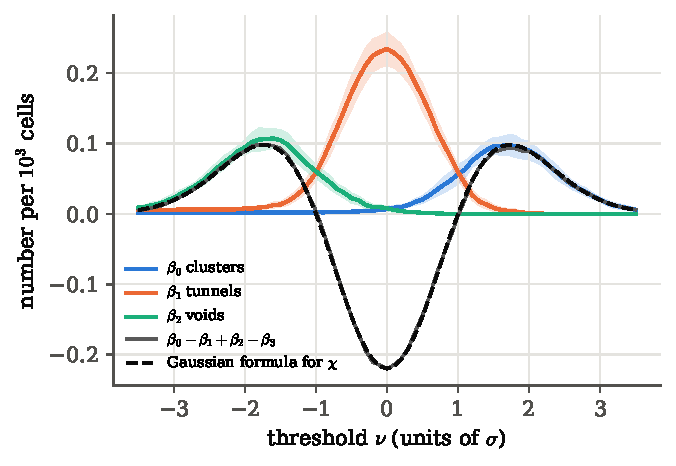
\includegraphics[width=0.62\linewidth]{figures/ch12/b_web_grf.pdf}
\caption{Betti curves of three-dimensional Gaussian boxes: clusters ($\beta_0$), tunnels ($\beta_1$) and voids
($\beta_2$) per thousand cells, mean of $\PbWebBoxes$ boxes with the box-to-box scatter shaded. The grey curve is
$\beta_0-\beta_1+\beta_2-\beta_3$ (the last term is the single three-dimensional class of the whole torus at the
lowest levels) and the dashed curve the Gaussian formula for the Euler characteristic.}
\label{12b:fig:web-grf}
\end{figure}

\Cref{12b:fig:web-grf} shows the result. The clusters peak at $\nu=\PbWebPeakZero$ with $\PbWebAmpZero$ per thousand
cells; the tunnels peak at $\nu=\PbWebPeakOne$, at $\PbWebAmpOne$ per thousand cells, more than twice as many as the
other two at their peaks; the voids peak at $\nu=\PbWebPeakTwo$ with $\PbWebAmpTwo$. The order is the one
\cref{12b:fig:events} predicts, and the symmetry is visible: the void curve is the mirror image of the cluster
curve, and the tunnel curve is centred on zero. The alternating sum agrees with the Gaussian formula for $\chi$
(\cref{12a:sec:gkf3}, \cref{T3a:eq:genus3d}) to within $\PbWebChiDev\%$ of its peak at every threshold, where one
Monte Carlo error is up to $\PbWebChiErr\%$; over all $\PbWebChiNpull$ thresholds the largest deviation is
$\PbWebChiPull$ of its own Monte Carlo errors. At this smoothing the finite cells, which the formula for a continuous field
does not know about, leave no visible trace.

\paragraph{Example: what $\chi$ hides at the median density.} At $\nu=0$ the Euler characteristic is $\PbWebChiZero$ per
thousand cells. Read alone, it says ``more tunnels than clusters and voids''. The Betti curves say how: at $\nu=0$ there
are $\PbWebBzeroAtZero$ clusters and $\PbWebBtwoAtZero$ voids per thousand cells, almost none, against $\PbWebAmpOne$
tunnels. At $\nu=+1.6$, where $\chi$ is $\PbWebChiPeak$, and at $-1.6$, where it has the same size, the curves say which
side we are on: at $+1.6$ the positive $\chi$ is clusters, at $-1.6$ it is voids. The
Euler characteristic cannot tell these two apart without the sign of $\nu$; for a non-Gaussian field, where the two
sides need not mirror each other, only the separate counts can.

\paragraph{Verification and research.} The agreement of the alternating sum with the formula verifies the code: it is
a known answer reproduced. The Betti curves themselves have no known answer. For Gaussian fields there are no exact
expressions for the expected Betti numbers, only approximations and numerical studies \cite{Pranav2017}, and for the
non-Gaussian density of the late universe there is nothing analytic at all. Here the Monte Carlo is not a check of
a formula but the only instrument we have: the expected curves and their scatter are whatever the simulations say,
and part~12c turns exactly these simulated means and covariances into a likelihood.

\subsection{What gravity does to the diagram}
\label{12b:sec:gravity}

The Gaussian box is the starting point of structure formation, not its result. \Cref{12a:sec:dynamics} drew the
distinction: a monotone relabelling of the density, such as $\delta\to e^{\delta}$, changes no excursion set and no
persistence pair beyond relabelling the levels (we checked this on a map in \cref{12b:sec:checks}), but gravitational
evolution moves matter around, merges structures and empties voids, so the topology itself changes. Wilding and
collaborators followed this in $\Lambda$CDM $N$-body simulations, computing the Betti curves and persistence diagrams
of the density estimated on the Delaunay tessellation of the particles at redshifts from $3.8$ to $0$
\cite{Wilding2021}. Their diagrams grow sharp apexes, and the apex of the cluster diagram sits at the density at
which matter detaches from the expansion and begins to collapse; the features near the apex form a self-similar
population that reflects the hierarchical growth of structure. The topology there is not a quantity protected from
the physics; it is the record of the physics. Reproducing those diagrams needs $N$-body simulations and the Delaunay
density estimate, far beyond laptop scale; \cref{12b:sec:repro-pranav} reproduces the simpler reference case
that the same group used to learn to read such diagrams, a random scatter of points.
\section{Polarization singularities: a charge that a remapping cannot change}
\label{12b:sec:polsing}

The CMB polarization at a point is a headless stick: a direction without an arrowhead, described by the Stokes
parameters $Q$ and $U$ combined into $P=Q+iU=|P|e^{2i\alpha}$, with $\alpha$ the angle of the stick
(\cref{T3a:eq:alpha}; see the cosmology notes for where the polarization comes from). Where $Q=U=0$ the stick has no
direction. Walk once around such a point and the stick turns by half a turn, with the walk or against it: the
\emph{index} of the singularity is $+\frac12$ or $-\frac12$ (\cref{T3a:sec:index}). \Cref{T3a:sec:density} counted them
on simulated maps and \cref{T3a:sec:lensing} showed, on lensed patches, that gravitational lensing moves them without
changing their indices. Treated as data, the singularities are a catalogue of points with charges $\pm\frac12$, and
the questions are the statistical ones: what exactly protects the
charges, how do we measure them on a pixel map, and when does the protection fail? In the language of
\cref{12a:sec:nuisance}, lensing is a nuisance operator $\mathcal N$ that acts by remapping the sky, and we want to know
precisely which statistics $T$ satisfy $T[\mathcal N[P]]=T[P]$ and under which conditions.

\paragraph{The question.} If a polarization map is deformed continuously, or remapped by $\bm x\mapsto\bm x+\bm d(\bm x)$,
which properties of its singularities are guaranteed to survive, which can change, and how do they change?

\subsection{Why the charge cannot change continuously}
\label{12b:sec:charge-integer}

Take a closed loop $\Gamma$ on which the polarization never vanishes, and define the charge inside it as the number of
turns of the stick along the loop,
\begin{equation}
  q(\Gamma)=\frac{1}{2\pi}\oint_\Gamma\dd\alpha=\frac{1}{4\pi}\oint_\Gamma\dd\arg P ,
  \label{12b:eq:charge}
\end{equation}
which is the sum of the indices of the singularities inside $\Gamma$ (\cite{VachaspatiLue2003}, their eq.~5). Now let
the map change continuously with a parameter $t$ (time, or the strength of a lensing deflection), $P_t$, and suppose
that no singularity crosses $\Gamma$ while $t$ changes, so $P_t\neq0$ on $\Gamma$ throughout.
\begin{align}
  q_t(\Gamma)
  &\eqby{1}\frac{1}{4\pi}\times(\text{a whole number of turns of }\arg P_t\text{ along }\Gamma)\times2\pi
   \in\tfrac12\Z\nonumber\\
  &\eqby{2}\text{a continuous function of }t\nonumber\\
  &\eqby{3}q_0(\Gamma)\quad\text{for all }t .
  \label{12b:eq:charge-const}
\end{align}
\begin{explain}
  \item Going once around $\Gamma$ brings $P_t$ back to its starting value, so its phase changes by $2\pi$ times a whole
        number, and \eqref{12b:eq:charge} divides by $4\pi$: $q$ is a multiple of $\frac12$.
  \item $\arg P_t$ at each point of $\Gamma$ changes continuously with $t$ because $P_t$ does and never passes through
        $0$ there, so the integral changes continuously.
  \item A continuous function whose values are restricted to the separated numbers $\dots,-\frac12,0,\frac12,\dots$
        cannot jump from one to another, so it is constant.
\end{explain}
So the total charge inside a fixed loop can change only when a singularity crosses the loop. Inside the loop,
singularities can move, and a $+\frac12$ and a $-\frac12$ can be created together or annihilate together, because that
leaves the total unchanged; a single charge can never appear or vanish on its own \cite{VachaspatiLue2003}.

\subsection{The index of a zero, and what a remapping does to it}
\label{12b:sec:index-det}

\emph{The simplest zero first.} Near a zero at the origin, $Q$ and $U$ both vanish linearly, so
$Q+iU\approx f(z)=c_1z+c_2\bar z$, with $z=x+iy$ and complex constants $c_1,c_2$. The real map
$(x,y)\mapsto(Q,U)$ has the Jacobian matrix $J$ with rows $\nabla Q$ and $\nabla U$. Its determinant is
\begin{align}
  \det J
  &\eqby{1}Q_xU_y-Q_yU_x\eqby{2}\operatorname{Im}\big(\overline{f_x}\,f_y\big)\nonumber\\
  &\eqby{3}\operatorname{Im}\big((\bar c_1+\bar c_2)(ic_1-ic_2)\big)\nonumber\\
  &\eqby{4}\operatorname{Re}\big(|c_1|^2-|c_2|^2+c_1\bar c_2-\bar c_1c_2\big)
   \eqby{5}|c_1|^2-|c_2|^2 .
  \label{12b:eq:detJ}
\end{align}
\begin{explain}
  \item The determinant of the $2\times2$ matrix with rows $(Q_x,Q_y)$ and $(U_x,U_y)$; subscripts are partial
        derivatives.
  \item With $f_x=Q_x+iU_x$ and $f_y=Q_y+iU_y$, the product $\overline{f_x}f_y=(Q_xQ_y+U_xU_y)+i(Q_xU_y-U_xQ_y)$.
  \item From $f=c_1(x+iy)+c_2(x-iy)$: $f_x=c_1+c_2$ and $f_y=ic_1-ic_2$.
  \item Multiply out and use $\operatorname{Im}(iw)=\operatorname{Re}w$.
  \item $c_1\bar c_2-\bar c_1c_2$ is a number minus its complex conjugate, which is purely imaginary.
\end{explain}
\emph{Which way does $P$ turn?} If $|c_1|>|c_2|$, write $f=c_1z\,(1+w)$ with $w=(c_2/c_1)(\bar z/z)$. On a circle
around the origin $|w|=|c_2/c_1|<1$, so $1+w$ stays in a disc around $1$ that does not contain $0$ and its phase returns
to where it started without turning; the phase of $f$ then turns exactly as $z$ does, once, with the loop. The index is
$+\frac12$. If $|c_2|>|c_1|$, the same argument with $f=c_2\bar z(1+\dots)$ gives one turn against the loop: index
$-\frac12$. With \eqref{12b:eq:detJ} both cases read
\begin{equation}
  \text{index of a zero}=\tfrac12\,\sgn\det J .
  \label{12b:eq:index-det}
\end{equation}
This is the rule the plaquette finder of \cref{T3a:sec:index} applies implicitly: summing the phase steps around a
$2\times2$ block measures the sign of the local Jacobian.

\emph{A remapping.} The remapped map is $\tilde P(\bm x)=P(\bm F(\bm x))$ with $\bm F(\bm x)=\bm x+\bm d(\bm x)$, and its
zeros are the points $\bm x_0$ with $\bm F(\bm x_0)=\bm y_0$ a zero of $P$. By the chain rule the Jacobian of $\tilde P$ at
$\bm x_0$ is $J(\bm y_0)\,\mathsf A(\bm x_0)$, where $\mathsf A=\Id+\partial\bm d$ is the Jacobian of the remapping, the
magnification matrix of lensing (\cref{T3a:sec:protect}). Then
\begin{align}
  \text{index of }\tilde P\text{ at }\bm x_0
  &\eqby{1}\tfrac12\,\sgn\det\big(J(\bm y_0)\mathsf A(\bm x_0)\big)
   \eqby{2}\tfrac12\,\sgn\det J(\bm y_0)\ \sgn\det\mathsf A(\bm x_0)\nonumber\\
  &\eqby{3}\sgn\det\mathsf A(\bm x_0)\times\big(\text{index of }P\text{ at }\bm y_0\big) .
  \label{12b:eq:index-remap}
\end{align}
\begin{explain}
  \item The rule \eqref{12b:eq:index-det} applied to $\tilde P$, whose Jacobian is $J\mathsf A$.
  \item The determinant of a product is the product of the determinants.
  \item The rule \eqref{12b:eq:index-det} read backwards for $P$ at $\bm y_0$.
\end{explain}
Where the remapping keeps orientation, $\det\mathsf A>0$, every zero keeps its index. Where the sky is folded over
itself, $\det\mathsf A<0$, the image is a mirror image and the index flips.

\emph{Folds create pairs.} If $\det\mathsf A>0$ everywhere, the remapping is one-to-one and each zero of $P$ has exactly
one image, with the same index. If the displacement is strong enough to fold the sky, a point $\bm y_0$ can have three
preimages: one before the fold, one inside it (with $\det\mathsf A<0$), one after it. Their indices are, by
\eqref{12b:eq:index-remap}, $+q$, $-q$, $+q$, which add up to $q$. The one-dimensional cartoon of
\cref{12b:fig:fold} shows why the signs alternate: the curve $F(x)$ must cross the level $y_0$ going up, then down, then
up again. Seen from the remapped sky, a fold has created a pair of opposite charges and kept the total. This is
the exact form of the statement that a continuous change can only create or annihilate pairs.

\begin{figure}[htbp]
\centering
\begin{tikzpicture}[x=0.7cm,y=0.55cm]
  \fill[black!8] (-0.84,-4.3) rectangle (0.84,4.3);
  \draw[faint,->] (-4.4,0) -- (4.6,0) node[lbl,anchor=north] {$x$};
  \draw[faint,->] (0,-4.4) -- (0,4.6) node[lbl,anchor=east] {$F(x)$};
  \draw[faint,dashed] (-4,-4) -- (4,4);
  \draw[form,domain=-4:4,samples=120] plot (\x,{\x-1.5*sin(\x r)});
  \draw[bdry,thin] (-4.4,0) -- (4.4,0);
  \foreach \x/\s in {-1.496/+,0/-,1.496/+}{
    \fill[bdryred] (\x,0) circle (2.5pt);
  }
  \node[lbl,font=\scriptsize,anchor=north east] at (-1.55,-0.1) {slope $>0$};
  \node[lbl,font=\scriptsize,anchor=south] at (0,0.95) {slope $<0$};
  \node[lbl,font=\scriptsize,anchor=south west] at (1.55,0.1) {slope $>0$};
  \node[lbl,font=\scriptsize,anchor=west] at (4.05,4.0) {$F(x)=x$};
  \node[lbl,font=\scriptsize,anchor=west] at (4.05,2.5) {$F(x)=x-1.5\sin x$};
\end{tikzpicture}
\caption{A one-dimensional remapping $F(x)=x-1.5\sin x$ that folds: in the shaded strip its slope is negative. The level
$F=0$ (red line), the position of one singularity of the original map, is reached at three points (dots) with slopes of
signs $+,-,+$. The three images carry indices $+q,-q,+q$, which add up to the original $q$. The dashed line is the
identity map, which has a single crossing.}
\label{12b:fig:fold}
\end{figure}

\subsection{Testing the protection on simulated maps}
\label{12b:sec:remap-test}

\pyname{code/ch12/b06_pol_remap.py} draws $\PbRmReal$ E-mode polarization maps on periodic $\PbRmSide^\circ\times
\PbRmSide^\circ$ patches with $\PbRmN^2$ pixels of $\PbRmPix'$, smoothed by a $\PbRmFwhm'$ beam, from the fiducial
$C_\ell^{EE}$; each has about $\PbRmNzero$ singularities. For each map it draws a smooth random potential, coherent over
about a degree, takes $\bm d$ as its gradient, and scales it so that the convergence $\kappa=-\frac12\nabla\cdot\bm d$
has a chosen root-mean-square value $\kappa_{\rm rms}$, from $0.03$ (the size of real CMB lensing on these scales) up to
$0.8$. The remapped maps $\tilde Q(\bm x)=Q(\bm x+\bm d)$ and $\tilde U(\bm x)=U(\bm x+\bm d)$ are computed by cubic
interpolation. (On the curved sky the polarization must also be carried from the displaced point by parallel transport
\cite{ChallinorChon2002}, \cref{T3a:sec:remap}; on a flat patch that step is the identity.) For every singularity of
the remapped map the code follows $\bm d$ to the point
$\bm x+\bm d(\bm x)$ and looks there for a singularity of the original map within a pixel and a half; it checks the
index rule \eqref{12b:eq:index-remap} with the sign of $\det\mathsf A$ at that point; and for every original singularity
it adds up the indices of all its images and compares with its own index.

\begin{figure}[htbp]
\centering
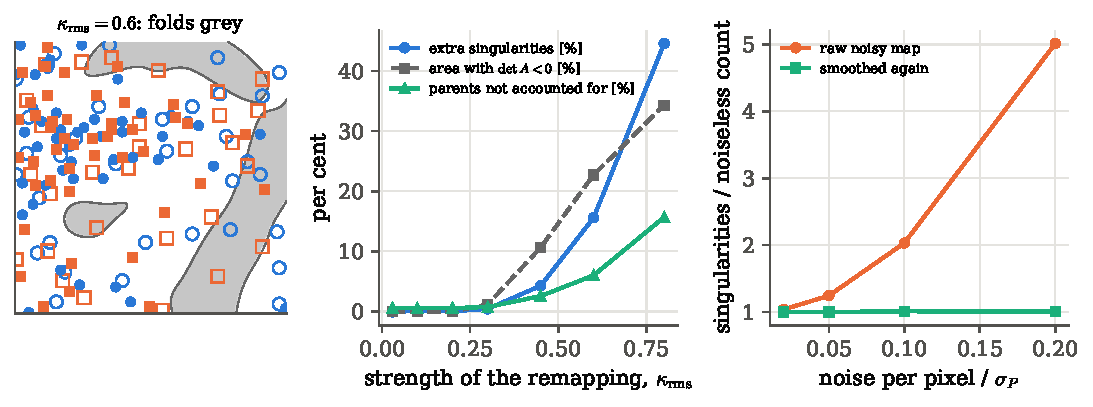
\includegraphics[width=\linewidth]{figures/ch12/b_remap.pdf}
\caption{Left: a $2.5^\circ\times2.5^\circ$ corner of one map remapped with $\kappa_{\rm rms}=0.6$; grey regions are
folded ($\det\mathsf A<0$). Open markers: singularities of the original map; filled: of the remapped map (circles
$+\frac12$, squares $-\frac12$). Middle: against the strength of the remapping, the fraction of extra singularities,
the folded area, and the fraction of original singularities whose images do not add up to their index. Right: noise is
not a remapping; white noise added to the map multiplies the number of singularities (orange), and smoothing the noisy
map again removes the extra ones (green).}
\label{12b:fig:remap}
\end{figure}

\paragraph{Example: realistic lensing strength.} At $\kappa_{\rm rms}=0.03$ no point of any map is folded. The remapped
maps have the same number of singularities as the originals (the change is $\PbRmExtraLow\%$); $\PbRmMatchLow\%$ of them sit
on an original singularity at the far end of their displacement, and $\PbRmRuleLow\%$ also carry the index the rule
\eqref{12b:eq:index-remap} predicts. The few exceptions are zeros that fall at the corner shared by two $2\times2$
blocks, where the pixel finder can put them in either block. This is the result of \cref{T3a:sec:lens-code} seen from
the other side: the catalogue of charges is unchanged, point by point, up to the resolution of the grid.

\paragraph{Example: folding the sky.} The first folds appear at $\kappa_{\rm rms}\approx\PbRmFirstFold$
(\cref{12b:fig:remap}, middle). At $\kappa_{\rm rms}=0.6$, $\PbRmFoldHigh\%$ of the area is folded and the remapped
maps have $\PbRmExtraHigh\%$ more singularities than the originals, all of them created in pairs, as the left panel
shows: inside and beside the grey regions, one original singularity has three images, the middle one with the opposite
index. For $\PbRmConsHigh\%$ of the original singularities the indices of the images still add up to the original
index, and $\PbRmRuleHigh\%$ of the images obey the sign rule. The failures grow with the folding because the remapped
field is squeezed near the fold lines, and some of the created pairs are closer together than a pixel: the grid can no
longer resolve them. Real CMB lensing, with a convergence of a few hundredths, is about ten times too weak to fold the sky; the experiment shows what the
protection rests on, and where it would end.

\paragraph{Example: noise is not a remapping.} White noise added to $Q$ and $U$ in each pixel, at a level of
$5\%$ of the polarization amplitude, raises the number of singularities by a factor $\PbNoiseRawFive$; at $20\%$, by a
factor $\PbNoiseRawTwenty$, and only $\PbNoiseMatchRawTwenty\%$ of the singularities of the noisy map lie on one of the
original map. The noise creates pairs on the scale of a pixel, wherever the polarization is weak. Smoothing the noisy map
over two pixels removes almost all of them: the count returns to $\PbNoiseSmTwenty$ times that of the equally smoothed
clean map, and $\PbNoiseMatchSmTwenty\%$ of the singularities match. The order matters, as \cref{T3a:sec:break} found
for the beam: a smoothing that acts on the remapped, noisy sky is part of the nuisance, and its effect must be measured by
simulating it.

\subsection{What is protected, and what is not}
\label{12b:sec:caveats}

Putting the pieces together, for a map changed by a smooth remapping or any continuous deformation:
\begin{itemize}[itemsep=1pt,leftmargin=1.2em]
  \item \emph{Protected:} the total charge inside any loop that no singularity crosses \eqref{12b:eq:charge-const}; and,
        while the remapping is one-to-one, the whole catalogue, singularity by singularity, with its indices
        \eqref{12b:eq:index-remap}.
  \item \emph{Not protected:} the positions (they move with the remapping); the number of singularities once folds
        appear (pairs are created); the charge inside a loop that singularities cross, which is the situation at the
        edge of any finite patch or mask; pairs closer than the resolution, which a beam or a pixel grid can merge or
        hide; and anything that noise touches, because noise is not a deformation of the map but an addition to it.
  \item \emph{A non-local step breaks it:} the $E$-mode and $B$-mode maps are built from $Q$ and $U$ by a non-local
        filter, so the singularities of an $E$-only map are not those of the full map and are not protected
        (\cref{T3a:sec:break}).
\end{itemize}
This is the caution of \cref{12a:sec:conditional} made concrete: a topological statistic is protected only against a
named class of transformations, and every analysis must say which class its nuisance belongs to.
\section{Reproducing the literature}
\label{12b:sec:repro}

Three papers carry the quantitative claims about persistence and singularities: Huterer and Vachaspati counted the polarization
singularities of simulated CMB maps and measured how their charges are arranged \cite{HutererVachaspati2005}, testing
a prediction of Vachaspati and Lue \cite{VachaspatiLue2003}; and Pranav and collaborators built the reference
Betti curves and diagrams against which the cosmic web is read \cite{Pranav2017}. We redo each of their measurements with our own
code, starting from what they asked and what they assumed, deriving the equation behind the number they plot, and then
putting their numbers next to ours and tracing every difference to a cause.

\subsection{How many singularities: Huterer and Vachaspati's counts}
\label{12b:sec:repro-hv}

\emph{Their question.} In 2004 the first CMB polarization maps were arriving, and Huterer and Vachaspati asked what
the singularities of a polarization map from the standard cosmological model should look like, so that the
predictions would be ready when the data were. The first number they report is the simplest: how many singularities a
full-sky map has, and how that grows with the angular resolution of the map.

\emph{Their setup.} They computed the spectra of a flat $\Lambda$CDM model with CMBFAST, drew Gaussian $E$ and $B$
coefficients from them up to a maximum multipole $\ell_{\max}$, made HEALPix maps at $N_{\rm side}=256$ and found the
singularities with the winding rule of \cref{T3a:sec:index}. With no tensor modes and no lensing, $C_\ell^{BB}=0$, so
the maps are pure $E$. Their parameters, as stated in the paper:

\begin{center}
\small
\begin{tabular}{lll}
\toprule
quantity & value & meaning\\
\midrule
$\Omega_m$ & $0.3$ & matter fraction of the critical density\\
$\Omega_mh^2$, $\Omega_bh^2$ & $0.127$, $0.021$ & physical matter and baryon densities ($h=\PbHvh$ follows)\\
$n_s$ & $1$ & primordial spectral index (scale-invariant)\\
tensors, lensing & none & so $B=0$\\
optical depth $\tau$ & not stated & sets the large-scale reionization signal in $C_\ell^{EE}$\\
\bottomrule
\end{tabular}
\end{center}

They found about $6000$ singularities for $\ell_{\max}=100$ and about $150\,000$ for $\ell_{\max}=500$, growing
``roughly as the square of'' $\ell_{\max}$.

\emph{Their key equation, here.} The paper gives no formula; the counts come from the maps. But the expected count
follows from the density formula derived in \cref{T3a:eq:density}, $n=\sigma_1^2/(4\pi\sigma_0^2)$ per steradian, with
$\sigma_0^2=\langle Q^2\rangle$ and $\sigma_1^2=\langle|\nabla Q|^2\rangle$. On a flat patch with pure $E$ modes, a Fourier
mode $\bm\ell$ of angle $\varphi_{\bm\ell}$ contributes $Q(\bm\ell)=E(\bm\ell)\cos2\varphi_{\bm\ell}$ (see the cosmology
notes for this relation), and a gradient brings down a factor $i\bm\ell$. So
\begin{align}
  \frac{\sigma_1^2}{\sigma_0^2}
  &\eqby{1}\frac{\int\frac{\dd^2\ell}{(2\pi)^2}\,\ell^2\,C_\ell^{EE}\cos^22\varphi_{\bm\ell}}
                {\int\frac{\dd^2\ell}{(2\pi)^2}\,C_\ell^{EE}\cos^22\varphi_{\bm\ell}}
   \eqby{2}\frac{\int_0^{\ell_{\max}}\ell^3C_\ell^{EE}\,\dd\ell}{\int_0^{\ell_{\max}}\ell\,C_\ell^{EE}\,\dd\ell}
   \equiv\langle\ell^2\rangle_E ,\nonumber\\
  N_{\rm sky}
  &\eqby{3}4\pi\,n\eqby{4}\langle\ell^2\rangle_E
   \;\longrightarrow\;\frac{\sum_{\ell}(2\ell+1)\,\ell(\ell+1)\,C_\ell^{EE}}{\sum_{\ell}(2\ell+1)\,C_\ell^{EE}} .
  \label{12b:eq:nsky}
\end{align}
\begin{explain}
  \item The variance of a Gaussian field is the integral of its spectrum over all modes; for the gradient each mode is
        weighted by $|i\bm\ell|^2=\ell^2$.
  \item Write $\dd^2\ell=\ell\,\dd\ell\,\dd\varphi$. The angular integral of $\cos^22\varphi$ is $\pi$ in both numerator
        and denominator and cancels, as do the $(2\pi)^2$; the spectrum is cut at $\ell_{\max}$.
  \item A full sky is $4\pi$ steradians.
  \item Insert $n=\sigma_1^2/(4\pi\sigma_0^2)$. The arrow is the same average written on the sphere, \cref{T3a:eq:Nsky},
        where a ring of $\dd\ell$ in the flat plane, of circumference $2\pi\ell$, becomes the $2\ell+1$ modes of each
        multipole, and $\ell^2$ becomes the eigenvalue $\ell(\ell+1)$ of the Laplacian.
\end{explain}
The number of singularities on the sky is the power-weighted average of $\ell(\ell+1)$ below $\ell_{\max}$. Because
$C_\ell^{EE}$ rises with $\ell$ up to the first acoustic peaks, most of the weight sits near the cut, the average is a
fixed fraction of $\ell_{\max}^2$, and that is the ``roughly as the square''.

\emph{What we compute.} \pyname{code/ch12/b07_hv_counts.py} runs CAMB for their model twice, once with an optical
depth $\tau=0.06$ and once with reionization switched off, since their $\tau$ is not given; evaluates \eqref{12b:eq:nsky}
for $\ell_{\max}$ from $50$ to $500$; and counts the singularities directly on $\PbHvNsim$ simulated
$\PbHvSide^\circ\times\PbHvSide^\circ$ periodic patches at each $\ell_{\max}$, with at least four pixels per half
wavelength, scaling the counts to the full sky. The grid version of \eqref{12b:eq:nsky}, the same average over the
discrete Fourier modes of the patch, matches the patch counts to $\PbHvGridDev\%$ at every $\ell_{\max}$, at most $\PbHvGridPull$ times the Monte Carlo error of
$\PbHvNsim$ patches. The same
formula with the fiducial \textit{Planck} spectra (\cref{7b:sec:camb}) repeats the numbers of \cref{T3a:sec:hv}.

\emph{Side by side.}
\begin{center}
\small
\begin{tabular}{lccccc}
\toprule
$\ell_{\max}$ & H\&V 2005 & \eqref{12b:eq:nsky}, $\tau=0.06$ & \eqref{12b:eq:nsky}, no reionization & our patches & fiducial \\
\midrule
100 & $\approx6000$ & $\PbHvFormHundred$ & $\PbHvNoreionHundred$ & $\PbHvSimHundred\pm\PbHvSimErrHundred$ & $\PbFidFormHundred$\\
500 & $\approx150\,000$ & $\PbHvFormFiveHundred$ & $\PbHvNoreionFiveHundred$ & $\PbHvSimFiveHundred\pm\PbHvSimErrFiveHundred$ & $\PbFidFormFiveHundred$\\
\bottomrule
\end{tabular}
\end{center}

\begin{figure}[htbp]
\centering
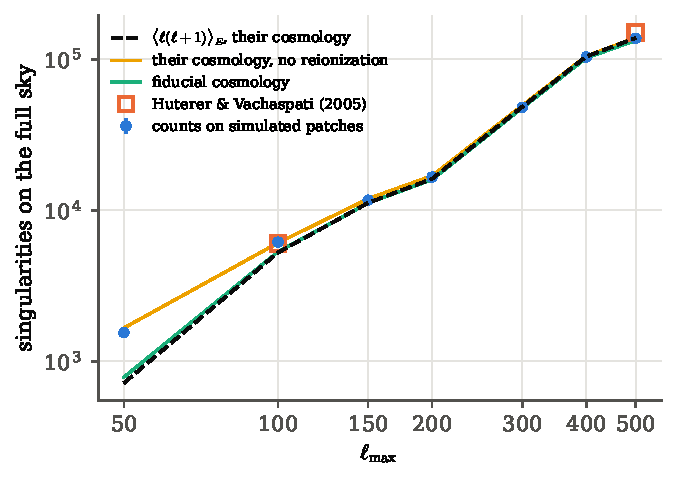
\includegraphics[width=0.62\linewidth]{figures/ch12/b_hv_counts.pdf}
\caption{Number of polarization singularities on the full sky against the maximum multipole of the map. Dashed: the
formula \eqref{12b:eq:nsky} for their cosmology with $\tau=0.06$; orange: the same without reionization; green: the
fiducial \textit{Planck} cosmology; dots: direct counts on simulated patches scaled to the full sky; squares: the two
numbers of Huterer and Vachaspati. The curves differ only at low $\ell_{\max}$, where the reionization signal at
$\ell<12$ carries a large share of the variance.}
\label{12b:fig:hv-counts}
\end{figure}

\emph{Why they differ.} At $\ell_{\max}=100$ the formula gives $\PbHvFormHundred$ with $\tau=0.06$ and
$\PbHvNoreionHundred$ without reionization: the reionization bump of $C_\ell^{EE}$ at $\ell<12$ adds variance $\sigma_0^2$
but almost no gradient variance $\sigma_1^2$, so it lowers the count by $14\%$. The published $6000$ is the
no-reionization number. Our patches agree with that number for a different reason: a $30^\circ$ patch cannot hold
modes with $\ell$ below about $360^\circ/30^\circ=12$, so it does not contain the bump at all
(\cref{12b:fig:hv-counts}; at $\ell_{\max}=50$ the patches follow the orange curve, $\PbHvNoreionFifty$, far from the
$\PbHvFormFifty$ of the dashed one). At $\ell_{\max}=500$ the bump no longer matters and the three numbers for their cosmology (formula with and
without reionization, and patches) agree to about one per cent; the published count is $8\%$ above them. We cannot trace that difference from the paper: their
value is quoted as a round number, their spectrum came from a different Boltzmann code, and their counting on HEALPix
pixels at $N_{\rm side}=256$ samples an $\ell_{\max}=500$ map with only about three pixels per wavelength. The growth
from $100$ to $500$ is a power $\ell_{\max}^{\PbHvSlope}$ in our formula, close to their ``square''.

\emph{The lesson.} Counting singularities measures one moment of the polarization spectrum, $\langle\ell(\ell+1)\rangle$,
and that moment is sensitive to whatever adds large-scale variance, here the reionization of the universe, which has
nothing to do with the small-scale structure where the singularities live. The count itself carries no information
beyond $C_\ell^{EE}$; any new information must be in how the charges are arranged, which the charge statistics below probe.

\subsection{How the charges are arranged: Vachaspati and Lue's exponent}
\label{12b:sec:repro-charge}

\emph{Their question.} Vachaspati and Lue noticed that a polarization map is a field of headless rods, like the
molecules of a nematic liquid crystal, and that the theory of defects in condensed matter predicts how the defects of
such a field are arranged \cite{VachaspatiLue2003}. The prediction concerns the net charge inside a large loop: it
fluctuates around zero, and its root-mean-square value should grow as the square root of the loop's length. Huterer and
Vachaspati measured the exponent on simulated maps \cite{HutererVachaspati2005}.

\emph{Their key equation, derived.} Take a loop $\Gamma$ of length $L$, much longer than the correlation length $\xi$
of the stick directions. Cut it into $m=L/\xi$ stretches of length $\xi$, and let $\delta\alpha_k$ be the change of the
stick angle along stretch $k$. By \eqref{12b:eq:charge} the charge inside is $q=\frac1{2\pi}\sum_k\delta\alpha_k$. The
increments have zero mean (no direction of turning is preferred), and increments along stretches farther apart than
$\xi$ are independent; call their common variance $s^2$. Then
\begin{align}
  \sigma^2(q)
  &\eqby{1}\frac{1}{4\pi^2}\Var\Big(\sum_{k=1}^{m}\delta\alpha_k\Big)
   \eqby{2}\frac{1}{4\pi^2}\sum_{k=1}^{m}\Var(\delta\alpha_k)
   \eqby{3}\frac{m\,s^2}{4\pi^2}=\frac{s^2}{4\pi^2}\,\frac{L}{\xi} ,\nonumber\\
  \sigma(q)&=\frac{s}{2\pi}\Big(\frac{L}{\xi}\Big)^{1/2}\qquad(\nu=\tfrac12).
  \label{12b:eq:nu-half}
\end{align}
\begin{explain}
  \item The variance of a constant times a random variable is the constant squared times its variance.
  \item The variance of a sum of independent terms is the sum of their variances (the covariances vanish).
  \item All $m$ terms have the same variance $s^2$, and $m=L/\xi$.
\end{explain}
This is \cite{VachaspatiLue2003}, their eq.~6, with $\beta=\frac12$. \emph{What the exponent means.} Compare a sky on
which the singularities were scattered at random with random signs, with density $n$. The charge inside a circle of
circumference $L$, area $A=L^2/4\pi$, would then be a sum of $\langle N\rangle=nA$ independent charges $\pm\frac12$:
\begin{align}
  \sigma^2(q)
  &\eqby{1}\langle N\rangle\,\Var(\pm\tfrac12)
   \eqby{2}\frac{nA}{4}
   \eqby{3}\frac{n\,L^2}{16\pi},\qquad \sigma(q)\propto L\quad(\nu=1).
  \label{12b:eq:nu-one}
\end{align}
\begin{explain}
  \item For a Poisson number of independent terms with zero mean, the variance of the sum is the mean number times the
        variance of one term.
  \item A charge $\pm\frac12$ with equal probabilities has variance $\frac14$.
  \item $A=\pi R^2$ and $L=2\pi R$ give $A=L^2/4\pi$.
\end{explain}
So $\nu=\frac12$ is the signature of charges that are not independent: a $+\frac12$ almost always has a $-\frac12$
nearby, and only the pairs that the loop cuts in two contribute to the net charge. Their number grows with the length
of the loop, not with its area. A measured $\nu$ near $\frac12$ says ``the charges are screened''; near $1$, ``they are
not''.

\emph{Their setup.} On a HEALPix map, the pixels of a ring at colatitude $\theta$ form a loop of length $L=2\pi\sin\theta$
around the north pole; the winding of the polarization angle along the ring gives the charge of the polar cap (with a
correction of one unit for the pole, where the local axes themselves turn once; it is the same for every map and
drops out of the spread). They rotated one map in a hundred random directions, measured $\sigma(q)$ ring by ring, and fit
$\sigma\propto L^\nu$ over rings plotted at $L=0.01,0.03,\dots,0.99$; values from $0.01$ to $1$ in equal steps match
$\sin\theta$, the ring length divided by $2\pi$, rather than the length itself, and we read their axis that way. They found $\nu=0.54$ for $\ell_{\max}=100$ and $\nu=0.45$ for
$\ell_{\max}=500$, each with an error of about $0.01$. They also measured the distance from each singularity to its
nearest neighbour of the same and of the opposite index, with means of $3.24^\circ$ and $2.69^\circ$ at
$\ell_{\max}=100$.

\emph{What we compute.} \pyname{code/ch12/b08_charge_stats.py} repeats their ring measurement on $\PbQnmap$
independent full-sky maps at $N_{\rm side}=\PbQnside$, their resolution, with their spectrum (without reionization,
which matched their counts in \cref{12b:sec:repro-hv}), at the $50$ rings with $\sin\theta=0.01,0.03,\dots,0.99$. The error on the fitted exponent comes from refitting it many
times on maps drawn at random, with repeats, from the $\PbQnmap$ (a bootstrap, \cref{3b:sec:bootstrap}). On periodic
$\PbQside^\circ$ flat patches it also catalogues the singularities themselves, measures the charge inside circles of
circumference $L$ with the true indices and with the indices shuffled among the singularities (which turns the
catalogue into the random-sign sky of \eqref{12b:eq:nu-one} at the same positions), and measures nearest-neighbour
distances.

\begin{figure}[htbp]
\centering
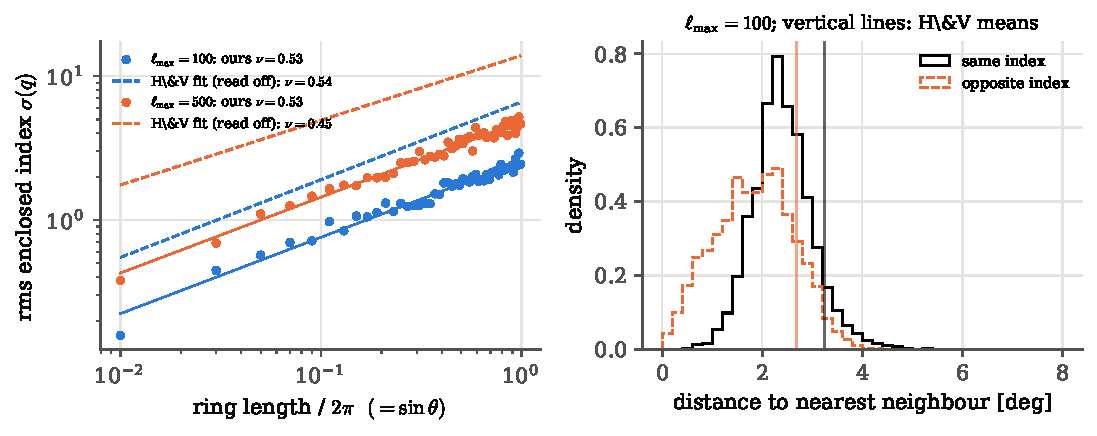
\includegraphics[width=\linewidth]{figures/ch12/b_charge_stats.pdf}
\caption{Left: root-mean-square charge of the polar caps against the ring length divided by $2\pi$, for maps cut at
$\ell_{\max}=100$ and $500$ (dots, with power-law fits), and the fitted laws of Huterer and Vachaspati read off their
figure (dashed). The slopes are close; the normalisations differ by a factor of two to three. Right: distance from each
singularity to its nearest neighbour of the same index and of the opposite index at $\ell_{\max}=100$; vertical lines
are their two means.}
\label{12b:fig:charge}
\end{figure}

\emph{Side by side.}
\begin{center}
\small
\begin{tabular}{lcc}
\toprule
 & H\&V 2005 & ours\\
\midrule
$\nu$, $\ell_{\max}=100$ (rings) & $0.54\pm0.01$ & $\PbNuHundred\pm\PbNuErrHundred$\\
$\nu$, $\ell_{\max}=500$ (rings) & $0.45\pm0.01$ & $\PbNuFiveHundred\pm\PbNuErrFiveHundred$\\
$\nu$ with indices shuffled, $\ell_{\max}=100$ / $500$ (patches) & -- & $\PbNuShufHundred$ / $\PbNuShufFiveHundred$\\
$\sigma(q)$ at $\sin\theta=1$, $\ell_{\max}=100$ / $500$ & $\approx7$ / $\approx14$ (read off) & $\PbSigHighHundred$ / $\PbSigHighFiveHundred$\\
nearest neighbour, same index & $3.24^\circ$ & $\PbNNsame^\circ$\\
nearest neighbour, opposite index & $2.69^\circ$ & $\PbNNopp^\circ$\\
ratio same / opposite & $1.20$ & $\PbNNratio$\\
\bottomrule
\end{tabular}
\end{center}

\begin{figure}[htbp]
\centering
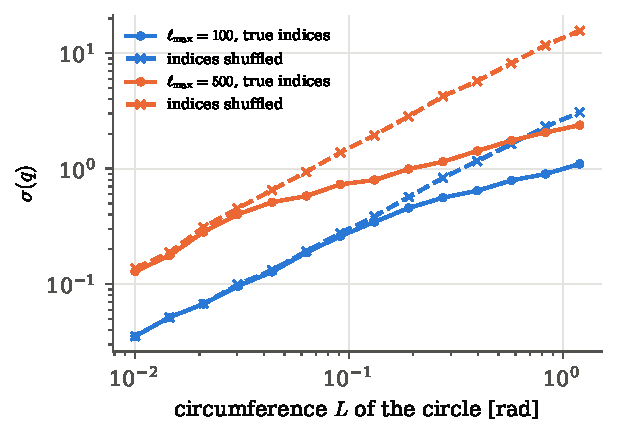
\includegraphics[width=0.55\linewidth]{figures/ch12/b_charge_shuffle.pdf}
\caption{Charge inside circles on flat patches, with the true indices (dots) and with the indices shuffled among the
same positions (crosses). For small circles, which hold at most one singularity, the two agree. For circles much longer
than the distance between a $+\frac12$ and its partner, the true charge grows as about $L^{1/2}$ and the shuffled one
as about $L$.}
\label{12b:fig:shuffle}
\end{figure}

\emph{Why they differ.} At $\ell_{\max}=100$ the two exponents differ by $\PbNuPullHundred$ combined standard errors. At
$\ell_{\max}=500$ ours is $\PbNuDiffFive$ higher, $\PbNuPullFive$ combined standard errors. Two things make the published error bar too small to judge either difference. Their hundred ring sets come from rotations
of one map, so they share that map's particular arrangement of charges, and the error of $0.01$ does not include the
scatter from one sky to another, which ours does. And $\sigma(q)$ is not an exact power of $L$: on small rings the cap
holds at most one singularity, and \eqref{12b:eq:nu-one} applies, with $\nu$ near $1$; only on rings much longer than the
pair separation does \eqref{12b:eq:nu-half} take over (\cref{12b:fig:shuffle}). The fitted slope depends on how much of
each regime the fit range contains, and it is noisy: on the patches, where we fit only circles longer than $0.2$
radians, the slope from one set of simulations to another scatters by about $\pm0.05$. The
normalisation is a separate matter. On the smallest ring, $\sin\theta=0.01$, the polar cap has an area of about
$\pi\times10^{-4}$ steradians, and with $\PbHvNoreionHundred$ singularities on $4\pi$ steradians it holds on average
$\PbHvNoreionHundred\times10^{-4}/4\approx0.15$ of them, so the charge there, made of independent single charges, has a spread of about
$\frac12\sqrt{0.15}\approx0.19$ in units of the fundamental charge $\frac12$, by \eqref{12b:eq:nu-one}; we measure
$\PbSigLowHundred$. Their figure shows about $0.4$ there, and the ratio stays between two and three at all lengths, so
their plotted charge must be in a different unit, which the paper does not state; a constant unit does not affect the
exponent. Finally, their nearest-neighbour distances are both about $1.4$ times ours, while the ratio of the two,
the measure of attraction against repulsion, is close ($1.20$ against $\PbNNratio$). Our distances are consistent with our
count: for random points at our density the mean nearest-neighbour distance would be $\PbNNrandom^\circ$, and we find
$\PbNNall^\circ$ to the nearest singularity of either index. Their own text quotes a mean nearest-neighbour distance
``slightly above $2^\circ$'' for about $6000$ singularities, where our maps with the same number give
$\PbNNall^\circ$, so their absolute distances belong to a sparser map than the one described, and cannot be compared
with ours; the qualitative result, opposite charges closer than equal ones, is reproduced.

\emph{The lesson.} The exponent $\nu$ is a slope fitted over a range of loop sizes on which the charge spread is not an
exact power law; its second decimal place depends on the range and on how many independent skies are used. What is
robust is the contrast between $\nu\approx\frac12$, screened charges born in pairs, and $\nu\approx1$, independent charges,
and the shuffling test shows that contrast directly.

\paragraph{A third look: the angular correlation function.} The charge spread looks at the net charge in a big loop, and
the nearest-neighbour distance at one singularity and its closest partner. A third question puts the two together:
at a separation $\theta$, are there more singularities, or fewer, than points thrown down at random would give, and
does the answer depend on the signs of the two charges? Huterer and Vachaspati answer with the angular correlation
function $w(\theta)$, borrowed from the clustering of galaxies. Its definition is a statement about pairs. If the
singularities were independent of each other, the chance that a given one has a second within a ring of
separations $[\theta_1,\theta_2]$ around it would just be the share of the sky inside the ring,
$f=\tfrac12(\cos\theta_1-\cos\theta_2)$ on a sphere, or $f=\pi(\theta_2^2-\theta_1^2)/A$ on a flat periodic patch of area
$A$. We then write the true chance as $f\,(1+w)$: $w=0$ is random, $w<0$ is repulsion, $w>0$ is attraction (their
eqs.~4--5). Counting over all pairs,
\begin{align}
  \text{pairs found in the ring}
  &\eqby{1}\frac{N(N-1)}{2}\,f\,\big(1+w(\theta)\big),\nonumber\\
  w(\theta)
  &\eqby{2}\frac{DD(\theta)}{RR(\theta)}-1 ,\qquad RR\equiv\frac{N(N-1)}{2}\,f .
  \label{12b:eq:wtheta}
\end{align}
\begin{explain}
  \item There are $N(N-1)/2$ pairs among $N$ singularities, and each lands in the ring with chance $f(1+w)$.
  \item $DD$ is the number of pairs in the data that fall in the ring and $RR$ the number a random scatter would
        give; solving for $w$ gives the Peebles--Hauser estimator \cite{HutererVachaspati2005} (their eq.~6, where the
        two numbers of points differ and so a ratio $N_{\rm rand}/N_{\rm map}$ appears). For pairs of equal charge the
        $N(N-1)/2$ is replaced by the number of such pairs, $N_+(N_+-1)/2+N_-(N_--1)/2$, and for opposite charges by
        $N_+N_-$.
\end{explain}
With no mask there is no selection function to model, and $RR$ is exact; the estimator needs no random catalogue.
\pyname{code/ch12/b09_wtheta.py} computes \eqref{12b:eq:wtheta} on $\PbWtNsim$ periodic $40^\circ$ patches at
$\ell_{\max}=100$ in bins of $2.5^\circ$ (\cref{12b:fig:wtheta}).

\begin{figure}[htbp]
\centering
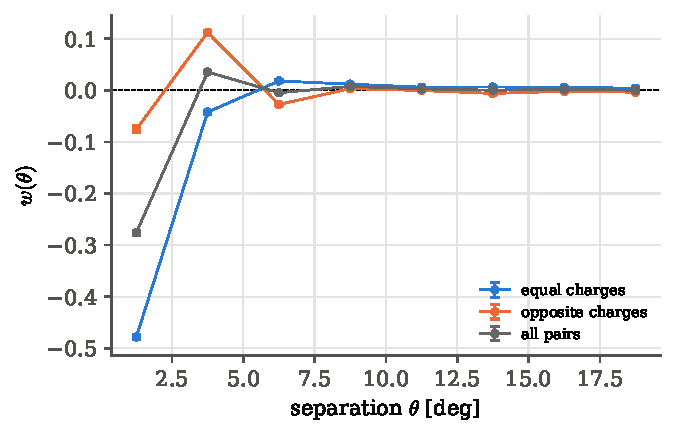
\includegraphics[width=0.55\linewidth]{figures/ch12/b_wtheta.pdf}
\caption{Angular correlation function of the singularities of $E$-mode maps cut at $\ell_{\max}=100$, mean of
$\PbWtNsim$ flat patches with the error of the mean, for all pairs and for pairs of equal and of opposite charge.
Closer than about $5^\circ$ equal charges are strongly deficient and opposite charges are in excess; beyond about
$10^\circ$ all three curves are flat at zero.}
\label{12b:fig:wtheta}
\end{figure}

In the first bin, closer than $2.5^\circ$, equal charges are almost absent ($w=\PbWtSame\pm\PbWtSameErr$) and
opposite charges are also deficient but much less so ($\PbWtOpp\pm\PbWtOppErr$); in the next bin, $2.5^\circ$ to
$5^\circ$, which is where the typical distance to the nearest partner sits, opposite charges are in excess and
equal charges are still deficient. Beyond $10^\circ$ every bin has $|w|\leq\PbWtFarMax$: the singularities are
placed as if at random. (The tiny positive values there are the counterpart of the deficit at short range, since the
pair counts of all bins must add up to $N(N-1)/2$.) This is their result: attraction of opposite and repulsion
of equal charges below about $10^\circ$, randomness above. Their bins have a half-width of $5^\circ$, four times the width of ours, so they cannot resolve the dip below
$2.5^\circ$ that the finer bins show; the two agree on the sign of the effect and on the scale, about $10^\circ$, at which it ends. On the physics: the correlation length of the polarization stick at $\ell_{\max}=100$ is a few
degrees, so there is nothing to correlate beyond it. They also repeated all these measurements for maps with a large tensor
fraction, a very tilted primordial spectrum ($n_s=0$ and $2$) and strongly skewed, non-Gaussian $a_{\ell m}$, and found $\nu$ and $w(\theta)$ unchanged
within errors, while the number of singularities changed with the total power; only a grossly anisotropic spectrum altered the statistics
\cite{HutererVachaspati2005}. We did not repeat these variations. The pairing of charges is a property of any smooth
random headless-vector field, not of a particular cosmology, and that is why these statistics hardly respond to the cosmological model.

\subsection{Betti curves of shot noise: Pranav and collaborators' baseline}
\label{12b:sec:repro-pranav}

\emph{Their question.} To read the Betti numbers and persistence diagrams of the real cosmic web one needs reference
cases where the answer is understood. Pranav and collaborators built such templates from simple point processes
\cite{Pranav2017}. They point out that even for a Gaussian random field no exact expressions for the Betti numbers or
the persistence diagrams exist, so the templates must be computed. The first template is the most featureless one:
points scattered uniformly at random, a Poisson process, whose topology is pure shot noise.

\emph{Their setup.} They put $500\,000$ particles at random in a periodic box of side $200\,h^{-1}$Mpc, estimated the
density at every particle with the Delaunay tessellation field estimator (DTFE, which uses the volume of the
tetrahedra around each particle), and computed the persistence of the superlevel sets. They plotted the Betti curves
against the density threshold divided by the standard deviation of the density, and reported that $\beta_0$ peaks at a
normalised level of about $1.8$, $\beta_1$ at $0.6$ and $\beta_2$ at $0.3$; that the three peaks are well separated, so
the topology is dominated in turn by clusters, tunnels and voids; and that for different mean separations of the
particles the normalised peak positions coincide.

\emph{Their key relation.} The Betti number at level $\nu$ is the number of diagram points with $b\geq\nu>d$
(their \S5.3), which is \eqref{12b:eq:betti-curve}; and the order of the peaks follows from \cref{12b:fig:events}.

\emph{What we compute.} The Poisson part of \pyname{code/ch12/b05_cosmic_web.py} puts particles at random in a periodic
box of $\PbPoisNg^3$ cells with mean separations of $2$, $3$ and $4$ cells (three realisations each), estimates the
density on the grid from the distance to the $\PbPoisK$th nearest particle, $\rho=\PbPoisK/(\frac43\pi r_{\PbPoisK}^3)$,
which adapts to the local density as the DTFE does, and computes the Betti curves of $\rho/\sigma_\rho$ with gudhi's
periodic cubical complex.

\begin{figure}[htbp]
\centering
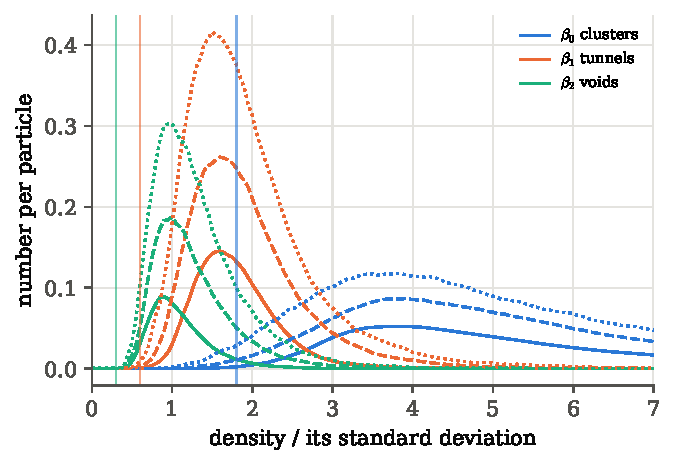
\includegraphics[width=0.62\linewidth]{figures/ch12/b_web_poisson.pdf}
\caption{Betti curves of the density of randomly placed points, per particle, against the density divided by its
standard deviation, for mean separations of $2$ (solid), $3$ (dashed) and $4$ (dotted) cells. Vertical lines: the peak
positions reported by Pranav and collaborators for their Delaunay density estimate. The order of the peaks and their
coincidence across separations are reproduced; the positions themselves depend on the estimator.}
\label{12b:fig:web-poisson}
\end{figure}

\emph{Side by side.}
\begin{center}
\small
\begin{tabular}{lcc}
\toprule
 & Pranav et al.\ 2017 (DTFE) & ours (nearest neighbours)\\
\midrule
peak of $\beta_0$ (clusters) & $\approx1.8$ & $\PbPoisPeakZero$\\
peak of $\beta_1$ (tunnels) & $\approx0.6$ & $\PbPoisPeakOne$\\
peak of $\beta_2$ (voids) & $\approx0.3$ & $\PbPoisPeakTwo$\\
order of the peaks & $\beta_0,\beta_1,\beta_2$ & $\beta_0,\beta_1,\beta_2$\\
peak positions for different separations & coincide & coincide within $\PbPoisSpread$\\
Gaussian field: exact Betti curves & none known & Monte Carlo, \cref{12b:fig:web-grf}\\
\bottomrule
\end{tabular}
\end{center}

\emph{Why they differ.} The levels are absolute densities in units of the standard deviation, not deviations from the
mean, so the peak positions depend on the ratio of the mean density to its spread, and that ratio belongs to the
estimator, not to the points. The DTFE gives very high densities to particles closely surrounded by others and very
low ones in empty regions, a broad distribution with a long tail; Pranav and collaborators note its tendency to form
spikes at clusters. Our nearest-neighbour estimate on a grid averages over five particles and is much narrower, so in
units of its own spread its mean sits higher and all three peaks move up. The order of the peaks and their independence
of the particle density do not depend on the estimator, and both are reproduced. The coincidence across separations is
not an accident: with the estimator tied to the mean separation, the density field of a Poisson process looks the same in
units of that separation, whatever its value.

\emph{The lesson.} A Betti curve of a point set describes the points and the estimator together. Two analyses can only
be compared, or a measurement compared with a model, if the simulated points go through the same density estimate as
the data: the same rule as for the beam and the noise in \cref{12b:sec:stability}.
\section{How it is done in research}
\label{12b:sec:research}

The Gaussian patches, boxes and random points of the experiments are scaled-down versions of analyses that are run in
research. The steps are the same; the data, the sizes and the care taken at each step are not. \Cref{12b:fig:pipeline}
lays out the pipeline as a real analysis runs it. Under each step of the pipeline we say what a real analysis involves, what
we did instead, and what the reduction costs.

\begin{figure}[htbp]
\centering
\begin{tikzpicture}[
  st/.style={draw=black!45,rounded corners=2pt,align=center,font=\footnotesize,text width=3.1cm,minimum height=1.25cm,
             fill=formblue!6},
  ck/.style={draw=bdryred!60,rounded corners=2pt,align=center,font=\scriptsize,text width=3.3cm,
             minimum height=0.9cm,fill=bdryred!4},
  arr/.style={->,thick,black!55}]
  \node[st] (d) at (0,0) {1. data product\\ \scriptsize maps, masks,\\ catalogues};
  \node[st] (f) at (3.7,0) {2. field or complex\\ \scriptsize smoothing,\\ density estimate};
  \node[st] (p) at (7.4,0) {3. persistence\\ \scriptsize diagrams,\\ singularities};
  \node[st] (s) at (11.1,0) {4. summary $S$\\ \scriptsize Betti curves,\\ $\nu$, counts};
  \node[st] (m) at (7.4,-2.6) {5. simulations\\ \scriptsize same pipeline,\\ steps 1--4};
  \node[st] (i) at (11.1,-2.6) {6. likelihood\\ \scriptsize $P(S\given\theta)$, part 12c};
  \draw[arr] (d) -- (f);
  \draw[arr] (f) -- (p);
  \draw[arr] (p) -- (s);
  \draw[arr] (s) -- (i);
  \draw[arr] (m) -- (i);
  \node[ck] (c1) at (1.7,-2.6) {checks: library against a small from-scratch run;\\ pixel convergence;\\ null tests};
  \draw[arr,dashed] (c1) -- (f);
  \draw[arr,dashed] (c1) -- (p);
\end{tikzpicture}
\caption{The pipeline of a persistence or singularity analysis. The data and every simulation go through exactly the
same steps 1--4; the simulations then give the sampling distribution of the summary, which part~12c turns into a
likelihood. The checks (red) guard the two steps where conventions are easiest to get wrong.}
\label{12b:fig:pipeline}
\end{figure}

\paragraph{1. Data products.} For CMB polarization the inputs are the component-separated $Q$ and $U$ maps of
\textit{Planck} (HEALPix, $N_{\rm side}=2048$), or arcminute-resolution maps from ground-based telescopes over part of the
sky, together with the mask of the Galaxy and point sources and a large set of end-to-end simulations of the
instrument's noise and processing (about a thousand for \textit{Planck}). For the cosmic web the inputs are galaxy
catalogues with positions and redshifts, or particle snapshots of $N$-body simulations; Wilding and collaborators used
five $\Lambda$CDM runs, each with $256^3$ particles in a box of $300\,h^{-1}$Mpc, at several redshifts
\cite{Wilding2021}. \emph{Ours:} Gaussian simulations only, flat patches of $10^\circ$ to $40^\circ$ and full-sky maps at
$N_{\rm side}=256$, periodic Gaussian boxes of $80^3$ cells and Poisson points on a $64^3$ grid. \emph{Cost:} no real
noise, no mask, no non-Gaussian structure; these are the baselines a real analysis compares against, not the analysis.

\paragraph{2. From data to a field or a complex.} Maps are smoothed to a common resolution chosen so that the pixel
noise is well below the field on that scale; \cref{12b:sec:stability} showed why: the stability theorem bounds the damage
by the largest noise value, and smoothing is what brings that value down. Particles are turned into a density by the
Delaunay tessellation field estimator, or the Delaunay tessellation itself becomes the complex (an alpha complex)
\cite{Pranav2017}. \emph{Ours:} Gaussian smoothing on a grid and a nearest-neighbour density. \emph{Cost:} the peak
positions of the Betti curves move with the estimator (\cref{12b:sec:repro-pranav}), so our curves are templates of the
same kind as the published ones, not the same templates.

\paragraph{3. Persistence and singularities.} On the sphere the cubical grid is replaced by HEALPix pixels with their
neighbours from \pyname{healpy.get_all_neighbours}, and persistence is computed with gudhi or a dedicated cubical code;
for $N$-body data, by the reduction of the Delaunay complex with PHAT \cite{Pranav2017,Wilding2021}. Polarization
singularities are found on HEALPix by following the polarization angle around small circuits of neighbouring pixels,
with the polarization at neighbouring pixels carried to a common tangent plane by parallel transport before the angles
are compared \cite{VachaspatiLue2003}, and with the correction at the poles of the coordinate system
\cite{HutererVachaspati2005}. The pixel size must resolve the map: Huterer and Vachaspati require
$N_{\rm side}>\ell_{\max}/4$. \emph{Ours:} flat periodic grids, where none of these geometric corrections arise, and
HEALPix rings only for the ring charges. \emph{Cost:} none in the statistics, which are local; but every geometric step we
skipped is a place where a real analysis can go wrong.

\paragraph{4. The summary.} A diagram is a set of points of varying number, which a likelihood cannot take directly. The
standard summaries are the Betti curves on a fixed grid of levels, histograms of the diagram points in birth--death bins
(the ``intensity maps'' of \cite{Pranav2017}), or smooth versions of them; for singularities, the counts by index, the
charge spread $\sigma(q)$ on a grid of loop sizes, nearest-neighbour statistics and the angular correlation function of
the singularities \cite{HutererVachaspati2005}. Each is a fixed-length vector $S$.

\paragraph{5. Simulations through the same pipeline.} Every effect we cannot model analytically, the mask cutting
features at its edges, the noise creating short bars and pairs of singularities, the beam merging them, the estimator,
is put into the simulations and goes through steps 1--4 unchanged. The simulated summaries give the mean and the
covariance of $S$ under each model. \emph{Ours:} a few dozen to a hundred realisations per measurement, each script under
ten minutes on a laptop. \emph{Cost:} Monte Carlo errors of a few per cent on means, as quoted with each result, and too
few realisations for an accurate covariance of a long summary vector, which part~12c addresses.

\paragraph{Checks.} Three checks recur in every serious analysis, and each appeared here. A library run is compared
with a from-scratch run on a small map (\cref{12b:sec:checks}), which catches mixed conventions. The pixel or particle
resolution is changed and the summary must not move (the count of singularities against pixel size,
\cref{12b:sec:repro-hv}). And null tests destroy the structure being measured while keeping everything else: shuffling
the indices among fixed positions (\cref{12b:fig:shuffle}) is one; rotating the map, or flipping the sign of a Gaussian
field, are others.

\begin{recap}
\begin{itemize}[itemsep=1pt,leftmargin=1.2em]
  \item Lowering a threshold through a field turns its excursion sets into a filtration. Each island, lake, tunnel or
        void has a birth level and a death level (\cref{12b:sec:filtration}); with the elder rule the record is unique.
        The persistence diagram is the set of pairs, the barcode draws them as intervals, and the Betti number at any
        level is the number of pairs alive there \eqref{12b:eq:betti-curve}. Persistence $b-d$ is the range of thresholds
        over which a feature exists.
  \item Stability: if the field changes by at most $\epsilon$ everywhere, the diagram moves by at most $\epsilon$ in the
        bottleneck distance; features created by the change have persistence at most $2\epsilon$ and sit by the diagonal
        (\cref{12b:sec:stability}). Verified on noisy maps: the ratio never exceeded $\PbStabMaxRatio$.
  \item Islands are computed by union--find with the elder rule, lakes by the same code on $-\phi$ with a sea around the
        map (Alexander duality in the plane, not on the torus); our code and gudhi, ripser, scipy and scikit-image agree
        exactly (\cref{12b:sec:compute}).
  \item For points, the Vietoris--Rips filtration; its island diagram is the minimum spanning tree (Kruskal, single
        linkage, friends-of-friends), and loops need the reduction of the boundary matrix (\cref{12b:sec:points}).
  \item In three dimensions clusters, tunnels and voids are born and die at maxima, filament saddles, wall saddles and
        minima; for a Gaussian field their curves peak at $\nu\approx\PbWebPeakZero$, $\PbWebPeakOne$ and
        $\PbWebPeakTwo$, and their alternating sum reproduces the Gaussian $\chi$ (\cref{12b:sec:web}). Gravity changes
        this topology; a monotone relabelling does not.
  \item The index of a polarization singularity is $\frac12\sgn\det J$; a remapping multiplies it by $\sgn\det\mathsf A$,
        so a one-to-one remapping keeps every charge, a fold creates pairs, and noise creates pairs on the pixel scale
        (\cref{12b:sec:polsing}).
  \item Reproduced: the singularity counts of Huterer and Vachaspati (the published $6000$ at $\ell_{\max}=100$ is the
        no-reionization value), the exponent $\nu\approx\frac12$ of Vachaspati and Lue and its meaning (screened pairs,
        against $\nu\approx1$ for shuffled charges), and the ordering of the Betti peaks of Pranav and collaborators
        (\cref{12b:sec:repro}).
\end{itemize}
\end{recap}
\providecommand{\WLam}{}\renewcommand{\WLam}{0.0452}
\providecommand{\WLamOmP}{}\renewcommand{\WLamOmP}{0.0465}
\providecommand{\WLamOmM}{}\renewcommand{\WLamOmM}{0.0437}
\providecommand{\WLamRatio}{}\renewcommand{\WLamRatio}{0.62}
\providecommand{\WSigPix}{}\renewcommand{\WSigPix}{0.0129}
\providecommand{\WRatioR}{}\renewcommand{\WRatioR}{0.29}
\providecommand{\WSkewTheory}{}\renewcommand{\WSkewTheory}{0.88}
\providecommand{\WSkewLog}{}\renewcommand{\WSkewLog}{0.88}
\providecommand{\WSkewLogErr}{}\renewcommand{\WSkewLogErr}{0.003}
\providecommand{\WSkewGauss}{}\renewcommand{\WSkewGauss}{0.001}
\providecommand{\WSkewLogSm}{}\renewcommand{\WSkewLogSm}{0.44}
\providecommand{\WSkewGaussSm}{}\renewcommand{\WSkewGaussSm}{0.001}
\providecommand{\WSigGTwo}{}\renewcommand{\WSigGTwo}{0.079}
\providecommand{\WPowDev}{}\renewcommand{\WPowDev}{1.1}
\providecommand{\WPowDevLow}{}\renewcommand{\WPowDevLow}{10.9}
\providecommand{\WPowDevG}{}\renewcommand{\WPowDevG}{10.2}
\providecommand{\WClipped}{}\renewcommand{\WClipped}{0.00}
\providecommand{\WMinLog}{}\renewcommand{\WMinLog}{-0.0356}
\providecommand{\WSigSm}{}\renewcommand{\WSigSm}{0.0064}
\providecommand{\WNsimOne}{}\renewcommand{\WNsimOne}{100}
\providecommand{\WRoundE}{}\renewcommand{\WRoundE}{2.7\times10^{-15}}
\providecommand{\WRoundB}{}\renewcommand{\WRoundB}{1.8\times10^{-15}}
\providecommand{\WGamRms}{}\renewcommand{\WGamRms}{0.0089}
\providecommand{\WKapRms}{}\renewcommand{\WKapRms}{0.0126}
\providecommand{\WSigPixNoise}{}\renewcommand{\WSigPixNoise}{0.0723}
\providecommand{\WNoiseRatioE}{}\renewcommand{\WNoiseRatioE}{1.002}
\providecommand{\WNoiseRatioB}{}\renewcommand{\WNoiseRatioB}{0.990}
\providecommand{\WNoisePow}{}\renewcommand{\WNoisePow}{9.95\times10^{-10}}
\providecommand{\WSigNLat}{}\renewcommand{\WSigNLat}{0.0102}
\providecommand{\WSigNCont}{}\renewcommand{\WSigNCont}{0.0102}
\providecommand{\WSigNMeas}{}\renewcommand{\WSigNMeas}{0.0102}
\providecommand{\WFobs}{}\renewcommand{\WFobs}{0.91}
\providecommand{\WErrNear}{}\renewcommand{\WErrNear}{0.37}
\providecommand{\WErrFar}{}\renewcommand{\WErrFar}{0.023}
\providecommand{\WBNear}{}\renewcommand{\WBNear}{0.36}
\providecommand{\WBFar}{}\renewcommand{\WBFar}{0.018}
\providecommand{\WLeakLow}{}\renewcommand{\WLeakLow}{2}
\providecommand{\WLeakHigh}{}\renewcommand{\WLeakHigh}{0.9}
\providecommand{\WSuppLow}{}\renewcommand{\WSuppLow}{0.90}
\providecommand{\WSuppHigh}{}\renewcommand{\WSuppHigh}{0.90}
\providecommand{\WBestDES}{}\renewcommand{\WBestDES}{4}
\providecommand{\WBestRDES}{}\renewcommand{\WBestRDES}{0.34}
\providecommand{\WBestKiDS}{}\renewcommand{\WBestKiDS}{4}
\providecommand{\WBestRKiDS}{}\renewcommand{\WBestRKiDS}{0.35}
\providecommand{\WBestSfour}{}\renewcommand{\WBestSfour}{2}
\providecommand{\WBestRSfour}{}\renewcommand{\WBestRSfour}{0.55}
\providecommand{\WBestDEShp}{}\renewcommand{\WBestDEShp}{5}
\providecommand{\WBestRDEShp}{}\renewcommand{\WBestRDEShp}{0.44}
\providecommand{\WBestSfourhp}{}\renewcommand{\WBestSfourhp}{2}
\providecommand{\WFobsT}{}\renewcommand{\WFobsT}{0.907}
\providecommand{\WBiasRawMin}{}\renewcommand{\WBiasRawMin}{-18}
\providecommand{\WBiasRawMax}{}\renewcommand{\WBiasRawMax}{-7}
\providecommand{\WBiasRescMax}{}\renewcommand{\WBiasRescMax}{10}
\providecommand{\WBiasDecMax}{}\renewcommand{\WBiasDecMax}{5.4}
\providecommand{\WErrDecMax}{}\renewcommand{\WErrDecMax}{3.1}
\providecommand{\WChiB}{}\renewcommand{\WChiB}{6.9}
\providecommand{\WNbands}{}\renewcommand{\WNbands}{8}
\providecommand{\WSdRatio}{}\renewcommand{\WSdRatio}{1.07}
\providecommand{\WLeakMax}{}\renewcommand{\WLeakMax}{1.3}
\providecommand{\WOffDiag}{}\renewcommand{\WOffDiag}{2}
\providecommand{\WSigOm}{}\renewcommand{\WSigOm}{0.097}
\providecommand{\WSigSe}{}\renewcommand{\WSigSe}{0.145}
\providecommand{\WRcorr}{}\renewcommand{\WRcorr}{-0.999}
\providecommand{\WSigSEight}{}\renewcommand{\WSigSEight}{0.0218}
\providecommand{\WSigSEightRel}{}\renewcommand{\WSigSEightRel}{2.6}
\providecommand{\WAlphaF}{}\renewcommand{\WAlphaF}{0.58}
\providecommand{\WFomCl}{}\renewcommand{\WFomCl}{1503}
\providecommand{\WSigSeFixed}{}\renewcommand{\WSigSeFixed}{0.0069}
\providecommand{\WSigSEightLow}{}\renewcommand{\WSigSEightLow}{0.0427}
\providecommand{\WSigSEightHigh}{}\renewcommand{\WSigSEightHigh}{0.0170}
\providecommand{\WSigSEightGrid}{}\renewcommand{\WSigSEightGrid}{0.0210}
\providecommand{\WSigOmGrid}{}\renewcommand{\WSigOmGrid}{0.099}
\providecommand{\WMargFactor}{}\renewcommand{\WMargFactor}{21.2}
\providecommand{\WNoiseN}{}\renewcommand{\WNoiseN}{9.95\times10^{-10}}
\providecommand{\WMcDiag}{}\renewcommand{\WMcDiag}{2.4}
\providecommand{\WNoiseMcDev}{}\renewcommand{\WNoiseMcDev}{0.76}
\providecommand{\WChiE}{}\renewcommand{\WChiE}{10.4}
\providecommand{\WToyOK}{}\renewcommand{\WToyOK}{agree}
\providecommand{\WGudhiDev}{}\renewcommand{\WGudhiDev}{0}
\providecommand{\WGudhiN}{}\renewcommand{\WGudhiN}{1600}
\providecommand{\WDevBzero}{}\renewcommand{\WDevBzero}{0}
\providecommand{\WDevChi}{}\renewcommand{\WDevChi}{0}
\providecommand{\WNpkClean}{}\renewcommand{\WNpkClean}{490}
\providecommand{\WNpkNoisy}{}\renewcommand{\WNpkNoisy}{685}
\providecommand{\WPkBoost}{}\renewcommand{\WPkBoost}{40}
\providecommand{\WNfidLN}{}\renewcommand{\WNfidLN}{1000}
\providecommand{\WNderLN}{}\renewcommand{\WNderLN}{800}
\providecommand{\WNfidG}{}\renewcommand{\WNfidG}{600}
\providecommand{\WNderG}{}\renewcommand{\WNderG}{400}
\providecommand{\WNmapsTot}{}\renewcommand{\WNmapsTot}{6400}
\providecommand{\WScale}{}\renewcommand{\WScale}{24.4}
\providecommand{\WDstep}{}\renewcommand{\WDstep}{10}
\providecommand{\WSigNoiseSm}{}\renewcommand{\WSigNoiseSm}{0.0102}
\providecommand{\WPall}{}\renewcommand{\WPall}{65}
\providecommand{\WHartAll}{}\renewcommand{\WHartAll}{0.93}
\providecommand{\WRunMin}{}\renewcommand{\WRunMin}{4.8}
\providecommand{\WPkLowSE}{}\renewcommand{\WPkLowSE}{0.060}
\providecommand{\WPkMidSE}{}\renewcommand{\WPkMidSE}{0.020}
\providecommand{\WPkHighSE}{}\renewcommand{\WPkHighSE}{0.014}
\providecommand{\WPkLowFom}{}\renewcommand{\WPkLowFom}{147}
\providecommand{\WPkMidFom}{}\renewcommand{\WPkMidFom}{545}
\providecommand{\WPkHighFom}{}\renewcommand{\WPkHighFom}{872}
\providecommand{\WLClP}{}\renewcommand{\WLClP}{8}
\providecommand{\WLClBias}{}\renewcommand{\WLClBias}{0.0}
\providecommand{\WLClSE}{}\renewcommand{\WLClSE}{0.0164}
\providecommand{\WLClOm}{}\renewcommand{\WLClOm}{0.065}
\providecommand{\WLClFom}{}\renewcommand{\WLClFom}{2321}
\providecommand{\WLClGain}{}\renewcommand{\WLClGain}{1.00}
\providecommand{\WLClSEgain}{}\renewcommand{\WLClSEgain}{0}
\providecommand{\WLClSERaw}{}\renewcommand{\WLClSERaw}{0.0164}
\providecommand{\WLClOmRaw}{}\renewcommand{\WLClOmRaw}{0.065}
\providecommand{\WLClFomRaw}{}\renewcommand{\WLClFomRaw}{2321}
\providecommand{\WLClGainRaw}{}\renewcommand{\WLClGainRaw}{1.00}
\providecommand{\WLClSEgainRaw}{}\renewcommand{\WLClSEgainRaw}{0}
\providecommand{\WLClSECmp}{}\renewcommand{\WLClSECmp}{0.0164}
\providecommand{\WLClOmCmp}{}\renewcommand{\WLClOmCmp}{0.065}
\providecommand{\WLClFomCmp}{}\renewcommand{\WLClFomCmp}{2321}
\providecommand{\WLClGainCmp}{}\renewcommand{\WLClGainCmp}{1.00}
\providecommand{\WLClSEgainCmp}{}\renewcommand{\WLClSEgainCmp}{-0}
\providecommand{\WLClR}{}\renewcommand{\WLClR}{-0.998}
\providecommand{\WLPkP}{}\renewcommand{\WLPkP}{11}
\providecommand{\WLPkBias}{}\renewcommand{\WLPkBias}{0.1}
\providecommand{\WLPkSE}{}\renewcommand{\WLPkSE}{0.0130}
\providecommand{\WLPkOm}{}\renewcommand{\WLPkOm}{0.069}
\providecommand{\WLPkFom}{}\renewcommand{\WLPkFom}{1796}
\providecommand{\WLPkGain}{}\renewcommand{\WLPkGain}{0.77}
\providecommand{\WLPkSEgain}{}\renewcommand{\WLPkSEgain}{20}
\providecommand{\WLPkSERaw}{}\renewcommand{\WLPkSERaw}{0.0127}
\providecommand{\WLPkOmRaw}{}\renewcommand{\WLPkOmRaw}{0.066}
\providecommand{\WLPkFomRaw}{}\renewcommand{\WLPkFomRaw}{1879}
\providecommand{\WLPkGainRaw}{}\renewcommand{\WLPkGainRaw}{0.81}
\providecommand{\WLPkSEgainRaw}{}\renewcommand{\WLPkSEgainRaw}{23}
\providecommand{\WLPkSECmp}{}\renewcommand{\WLPkSECmp}{0.0135}
\providecommand{\WLPkOmCmp}{}\renewcommand{\WLPkOmCmp}{0.073}
\providecommand{\WLPkFomCmp}{}\renewcommand{\WLPkFomCmp}{1704}
\providecommand{\WLPkGainCmp}{}\renewcommand{\WLPkGainCmp}{0.73}
\providecommand{\WLPkSEgainCmp}{}\renewcommand{\WLPkSEgainCmp}{17}
\providecommand{\WLPkR}{}\renewcommand{\WLPkR}{-0.997}
\providecommand{\WLMfP}{}\renewcommand{\WLMfP}{30}
\providecommand{\WLMfBias}{}\renewcommand{\WLMfBias}{0.4}
\providecommand{\WLMfSE}{}\renewcommand{\WLMfSE}{0.0127}
\providecommand{\WLMfOm}{}\renewcommand{\WLMfOm}{0.059}
\providecommand{\WLMfFom}{}\renewcommand{\WLMfFom}{2318}
\providecommand{\WLMfGain}{}\renewcommand{\WLMfGain}{1.00}
\providecommand{\WLMfSEgain}{}\renewcommand{\WLMfSEgain}{23}
\providecommand{\WLMfSERaw}{}\renewcommand{\WLMfSERaw}{0.0114}
\providecommand{\WLMfOmRaw}{}\renewcommand{\WLMfOmRaw}{0.050}
\providecommand{\WLMfFomRaw}{}\renewcommand{\WLMfFomRaw}{2743}
\providecommand{\WLMfGainRaw}{}\renewcommand{\WLMfGainRaw}{1.18}
\providecommand{\WLMfSEgainRaw}{}\renewcommand{\WLMfSEgainRaw}{30}
\providecommand{\WLMfSECmp}{}\renewcommand{\WLMfSECmp}{0.0130}
\providecommand{\WLMfOmCmp}{}\renewcommand{\WLMfOmCmp}{0.062}
\providecommand{\WLMfFomCmp}{}\renewcommand{\WLMfFomCmp}{2218}
\providecommand{\WLMfGainCmp}{}\renewcommand{\WLMfGainCmp}{0.96}
\providecommand{\WLMfSEgainCmp}{}\renewcommand{\WLMfSEgainCmp}{21}
\providecommand{\WLMfR}{}\renewcommand{\WLMfR}{-0.996}
\providecommand{\WLBettiP}{}\renewcommand{\WLBettiP}{20}
\providecommand{\WLBettiBias}{}\renewcommand{\WLBettiBias}{0.4}
\providecommand{\WLBettiSE}{}\renewcommand{\WLBettiSE}{0.0184}
\providecommand{\WLBettiOm}{}\renewcommand{\WLBettiOm}{0.093}
\providecommand{\WLBettiFom}{}\renewcommand{\WLBettiFom}{1150}
\providecommand{\WLBettiGain}{}\renewcommand{\WLBettiGain}{0.50}
\providecommand{\WLBettiSEgain}{}\renewcommand{\WLBettiSEgain}{-13}
\providecommand{\WLBettiSERaw}{}\renewcommand{\WLBettiSERaw}{0.0158}
\providecommand{\WLBettiOmRaw}{}\renewcommand{\WLBettiOmRaw}{0.074}
\providecommand{\WLBettiFomRaw}{}\renewcommand{\WLBettiFomRaw}{1437}
\providecommand{\WLBettiGainRaw}{}\renewcommand{\WLBettiGainRaw}{0.62}
\providecommand{\WLBettiSEgainRaw}{}\renewcommand{\WLBettiSEgainRaw}{4}
\providecommand{\WLBettiSECmp}{}\renewcommand{\WLBettiSECmp}{0.0202}
\providecommand{\WLBettiOmCmp}{}\renewcommand{\WLBettiOmCmp}{0.105}
\providecommand{\WLBettiFomCmp}{}\renewcommand{\WLBettiFomCmp}{1019}
\providecommand{\WLBettiGainCmp}{}\renewcommand{\WLBettiGainCmp}{0.44}
\providecommand{\WLBettiSEgainCmp}{}\renewcommand{\WLBettiSEgainCmp}{-23}
\providecommand{\WLBettiR}{}\renewcommand{\WLBettiR}{-0.998}
\providecommand{\WLPbettiP}{}\renewcommand{\WLPbettiP}{26}
\providecommand{\WLPbettiBias}{}\renewcommand{\WLPbettiBias}{0.7}
\providecommand{\WLPbettiSE}{}\renewcommand{\WLPbettiSE}{0.0173}
\providecommand{\WLPbettiOm}{}\renewcommand{\WLPbettiOm}{0.090}
\providecommand{\WLPbettiFom}{}\renewcommand{\WLPbettiFom}{1141}
\providecommand{\WLPbettiGain}{}\renewcommand{\WLPbettiGain}{0.49}
\providecommand{\WLPbettiSEgain}{}\renewcommand{\WLPbettiSEgain}{-5}
\providecommand{\WLPbettiSERaw}{}\renewcommand{\WLPbettiSERaw}{0.0148}
\providecommand{\WLPbettiOmRaw}{}\renewcommand{\WLPbettiOmRaw}{0.070}
\providecommand{\WLPbettiFomRaw}{}\renewcommand{\WLPbettiFomRaw}{1480}
\providecommand{\WLPbettiGainRaw}{}\renewcommand{\WLPbettiGainRaw}{0.64}
\providecommand{\WLPbettiSEgainRaw}{}\renewcommand{\WLPbettiSEgainRaw}{10}
\providecommand{\WLPbettiSECmp}{}\renewcommand{\WLPbettiSECmp}{0.0207}
\providecommand{\WLPbettiOmCmp}{}\renewcommand{\WLPbettiOmCmp}{0.116}
\providecommand{\WLPbettiFomCmp}{}\renewcommand{\WLPbettiFomCmp}{888}
\providecommand{\WLPbettiGainCmp}{}\renewcommand{\WLPbettiGainCmp}{0.38}
\providecommand{\WLPbettiSEgainCmp}{}\renewcommand{\WLPbettiSEgainCmp}{-26}
\providecommand{\WLPbettiR}{}\renewcommand{\WLPbettiR}{-0.997}
\providecommand{\WLClPkP}{}\renewcommand{\WLClPkP}{19}
\providecommand{\WLClPkBias}{}\renewcommand{\WLClPkBias}{0.1}
\providecommand{\WLClPkSE}{}\renewcommand{\WLClPkSE}{0.0112}
\providecommand{\WLClPkOm}{}\renewcommand{\WLClPkOm}{0.043}
\providecommand{\WLClPkFom}{}\renewcommand{\WLClPkFom}{3586}
\providecommand{\WLClPkGain}{}\renewcommand{\WLClPkGain}{1.55}
\providecommand{\WLClPkSEgain}{}\renewcommand{\WLClPkSEgain}{31}
\providecommand{\WLClPkSERaw}{}\renewcommand{\WLClPkSERaw}{0.0111}
\providecommand{\WLClPkOmRaw}{}\renewcommand{\WLClPkOmRaw}{0.042}
\providecommand{\WLClPkFomRaw}{}\renewcommand{\WLClPkFomRaw}{3654}
\providecommand{\WLClPkGainRaw}{}\renewcommand{\WLClPkGainRaw}{1.57}
\providecommand{\WLClPkSEgainRaw}{}\renewcommand{\WLClPkSEgainRaw}{32}
\providecommand{\WLClPkSECmp}{}\renewcommand{\WLClPkSECmp}{0.0115}
\providecommand{\WLClPkOmCmp}{}\renewcommand{\WLClPkOmCmp}{0.044}
\providecommand{\WLClPkFomCmp}{}\renewcommand{\WLClPkFomCmp}{3481}
\providecommand{\WLClPkGainCmp}{}\renewcommand{\WLClPkGainCmp}{1.50}
\providecommand{\WLClPkSEgainCmp}{}\renewcommand{\WLClPkSEgainCmp}{30}
\providecommand{\WLClPkR}{}\renewcommand{\WLClPkR}{-0.995}
\providecommand{\WLClMfP}{}\renewcommand{\WLClMfP}{38}
\providecommand{\WLClMfBias}{}\renewcommand{\WLClMfBias}{0.3}
\providecommand{\WLClMfSE}{}\renewcommand{\WLClMfSE}{0.0111}
\providecommand{\WLClMfOm}{}\renewcommand{\WLClMfOm}{0.042}
\providecommand{\WLClMfFom}{}\renewcommand{\WLClMfFom}{3701}
\providecommand{\WLClMfGain}{}\renewcommand{\WLClMfGain}{1.59}
\providecommand{\WLClMfSEgain}{}\renewcommand{\WLClMfSEgain}{32}
\providecommand{\WLClMfSERaw}{}\renewcommand{\WLClMfSERaw}{0.0105}
\providecommand{\WLClMfOmRaw}{}\renewcommand{\WLClMfOmRaw}{0.038}
\providecommand{\WLClMfFomRaw}{}\renewcommand{\WLClMfFomRaw}{4059}
\providecommand{\WLClMfGainRaw}{}\renewcommand{\WLClMfGainRaw}{1.75}
\providecommand{\WLClMfSEgainRaw}{}\renewcommand{\WLClMfSEgainRaw}{36}
\providecommand{\WLClMfSECmp}{}\renewcommand{\WLClMfSECmp}{0.0113}
\providecommand{\WLClMfOmCmp}{}\renewcommand{\WLClMfOmCmp}{0.043}
\providecommand{\WLClMfFomCmp}{}\renewcommand{\WLClMfFomCmp}{3578}
\providecommand{\WLClMfGainCmp}{}\renewcommand{\WLClMfGainCmp}{1.54}
\providecommand{\WLClMfSEgainCmp}{}\renewcommand{\WLClMfSEgainCmp}{31}
\providecommand{\WLClMfR}{}\renewcommand{\WLClMfR}{-0.995}
\providecommand{\WLClBettiP}{}\renewcommand{\WLClBettiP}{28}
\providecommand{\WLClBettiBias}{}\renewcommand{\WLClBettiBias}{0.2}
\providecommand{\WLClBettiSE}{}\renewcommand{\WLClBettiSE}{0.0132}
\providecommand{\WLClBettiOm}{}\renewcommand{\WLClBettiOm}{0.051}
\providecommand{\WLClBettiFom}{}\renewcommand{\WLClBettiFom}{2991}
\providecommand{\WLClBettiGain}{}\renewcommand{\WLClBettiGain}{1.29}
\providecommand{\WLClBettiSEgain}{}\renewcommand{\WLClBettiSEgain}{20}
\providecommand{\WLClBettiSERaw}{}\renewcommand{\WLClBettiSERaw}{0.0124}
\providecommand{\WLClBettiOmRaw}{}\renewcommand{\WLClBettiOmRaw}{0.047}
\providecommand{\WLClBettiFomRaw}{}\renewcommand{\WLClBettiFomRaw}{3243}
\providecommand{\WLClBettiGainRaw}{}\renewcommand{\WLClBettiGainRaw}{1.40}
\providecommand{\WLClBettiSEgainRaw}{}\renewcommand{\WLClBettiSEgainRaw}{24}
\providecommand{\WLClBettiSECmp}{}\renewcommand{\WLClBettiSECmp}{0.0139}
\providecommand{\WLClBettiOmCmp}{}\renewcommand{\WLClBettiOmCmp}{0.055}
\providecommand{\WLClBettiFomCmp}{}\renewcommand{\WLClBettiFomCmp}{2775}
\providecommand{\WLClBettiGainCmp}{}\renewcommand{\WLClBettiGainCmp}{1.20}
\providecommand{\WLClBettiSEgainCmp}{}\renewcommand{\WLClBettiSEgainCmp}{15}
\providecommand{\WLClBettiR}{}\renewcommand{\WLClBettiR}{-0.996}
\providecommand{\WLClPbettiP}{}\renewcommand{\WLClPbettiP}{34}
\providecommand{\WLClPbettiBias}{}\renewcommand{\WLClPbettiBias}{0.3}
\providecommand{\WLClPbettiSE}{}\renewcommand{\WLClPbettiSE}{0.0131}
\providecommand{\WLClPbettiOm}{}\renewcommand{\WLClPbettiOm}{0.050}
\providecommand{\WLClPbettiFom}{}\renewcommand{\WLClPbettiFom}{3022}
\providecommand{\WLClPbettiGain}{}\renewcommand{\WLClPbettiGain}{1.30}
\providecommand{\WLClPbettiSEgain}{}\renewcommand{\WLClPbettiSEgain}{20}
\providecommand{\WLClPbettiSERaw}{}\renewcommand{\WLClPbettiSERaw}{0.0122}
\providecommand{\WLClPbettiOmRaw}{}\renewcommand{\WLClPbettiOmRaw}{0.046}
\providecommand{\WLClPbettiFomRaw}{}\renewcommand{\WLClPbettiFomRaw}{3337}
\providecommand{\WLClPbettiGainRaw}{}\renewcommand{\WLClPbettiGainRaw}{1.44}
\providecommand{\WLClPbettiSEgainRaw}{}\renewcommand{\WLClPbettiSEgainRaw}{26}
\providecommand{\WLClPbettiSECmp}{}\renewcommand{\WLClPbettiSECmp}{0.0144}
\providecommand{\WLClPbettiOmCmp}{}\renewcommand{\WLClPbettiOmCmp}{0.057}
\providecommand{\WLClPbettiFomCmp}{}\renewcommand{\WLClPbettiFomCmp}{2662}
\providecommand{\WLClPbettiGainCmp}{}\renewcommand{\WLClPbettiGainCmp}{1.15}
\providecommand{\WLClPbettiSEgainCmp}{}\renewcommand{\WLClPbettiSEgainCmp}{12}
\providecommand{\WLClPbettiR}{}\renewcommand{\WLClPbettiR}{-0.996}
\providecommand{\WLAllP}{}\renewcommand{\WLAllP}{65}
\providecommand{\WLAllBias}{}\renewcommand{\WLAllBias}{0.7}
\providecommand{\WLAllSE}{}\renewcommand{\WLAllSE}{0.0109}
\providecommand{\WLAllOm}{}\renewcommand{\WLAllOm}{0.041}
\providecommand{\WLAllFom}{}\renewcommand{\WLAllFom}{3781}
\providecommand{\WLAllGain}{}\renewcommand{\WLAllGain}{1.63}
\providecommand{\WLAllSEgain}{}\renewcommand{\WLAllSEgain}{33}
\providecommand{\WLAllSERaw}{}\renewcommand{\WLAllSERaw}{0.0100}
\providecommand{\WLAllOmRaw}{}\renewcommand{\WLAllOmRaw}{0.035}
\providecommand{\WLAllFomRaw}{}\renewcommand{\WLAllFomRaw}{4391}
\providecommand{\WLAllGainRaw}{}\renewcommand{\WLAllGainRaw}{1.89}
\providecommand{\WLAllSEgainRaw}{}\renewcommand{\WLAllSEgainRaw}{39}
\providecommand{\WLAllSECmp}{}\renewcommand{\WLAllSECmp}{0.0116}
\providecommand{\WLAllOmCmp}{}\renewcommand{\WLAllOmCmp}{0.044}
\providecommand{\WLAllFomCmp}{}\renewcommand{\WLAllFomCmp}{3454}
\providecommand{\WLAllGainCmp}{}\renewcommand{\WLAllGainCmp}{1.49}
\providecommand{\WLAllSEgainCmp}{}\renewcommand{\WLAllSEgainCmp}{29}
\providecommand{\WLAllR}{}\renewcommand{\WLAllR}{-0.994}
\providecommand{\WGClP}{}\renewcommand{\WGClP}{8}
\providecommand{\WGClBias}{}\renewcommand{\WGClBias}{0.0}
\providecommand{\WGClSE}{}\renewcommand{\WGClSE}{0.0164}
\providecommand{\WGClOm}{}\renewcommand{\WGClOm}{0.066}
\providecommand{\WGClFom}{}\renewcommand{\WGClFom}{2207}
\providecommand{\WGClGain}{}\renewcommand{\WGClGain}{1.00}
\providecommand{\WGClSEgain}{}\renewcommand{\WGClSEgain}{0}
\providecommand{\WGClSERaw}{}\renewcommand{\WGClSERaw}{0.0164}
\providecommand{\WGClOmRaw}{}\renewcommand{\WGClOmRaw}{0.066}
\providecommand{\WGClFomRaw}{}\renewcommand{\WGClFomRaw}{2208}
\providecommand{\WGClGainRaw}{}\renewcommand{\WGClGainRaw}{1.00}
\providecommand{\WGClSEgainRaw}{}\renewcommand{\WGClSEgainRaw}{0}
\providecommand{\WGClSECmp}{}\renewcommand{\WGClSECmp}{0.0164}
\providecommand{\WGClOmCmp}{}\renewcommand{\WGClOmCmp}{0.066}
\providecommand{\WGClFomCmp}{}\renewcommand{\WGClFomCmp}{2207}
\providecommand{\WGClGainCmp}{}\renewcommand{\WGClGainCmp}{1.00}
\providecommand{\WGClSEgainCmp}{}\renewcommand{\WGClSEgainCmp}{-0}
\providecommand{\WGClR}{}\renewcommand{\WGClR}{-0.998}
\providecommand{\WGPkP}{}\renewcommand{\WGPkP}{11}
\providecommand{\WGPkBias}{}\renewcommand{\WGPkBias}{0.3}
\providecommand{\WGPkSE}{}\renewcommand{\WGPkSE}{nan}
\providecommand{\WGPkOm}{}\renewcommand{\WGPkOm}{nan}
\providecommand{\WGPkFom}{}\renewcommand{\WGPkFom}{nan}
\providecommand{\WGPkGain}{}\renewcommand{\WGPkGain}{nan}
\providecommand{\WGPkSEgain}{}\renewcommand{\WGPkSEgain}{nan}
\providecommand{\WGPkSERaw}{}\renewcommand{\WGPkSERaw}{0.0431}
\providecommand{\WGPkOmRaw}{}\renewcommand{\WGPkOmRaw}{0.239}
\providecommand{\WGPkFomRaw}{}\renewcommand{\WGPkFomRaw}{508}
\providecommand{\WGPkGainRaw}{}\renewcommand{\WGPkGainRaw}{0.23}
\providecommand{\WGPkSEgainRaw}{}\renewcommand{\WGPkSEgainRaw}{-163}
\providecommand{\WGPkSECmp}{}\renewcommand{\WGPkSECmp}{0.8417}
\providecommand{\WGPkOmCmp}{}\renewcommand{\WGPkOmCmp}{4.748}
\providecommand{\WGPkFomCmp}{}\renewcommand{\WGPkFomCmp}{26}
\providecommand{\WGPkGainCmp}{}\renewcommand{\WGPkGainCmp}{0.01}
\providecommand{\WGPkSEgainCmp}{}\renewcommand{\WGPkSEgainCmp}{-5038}
\providecommand{\WGPkR}{}\renewcommand{\WGPkR}{nan}
\providecommand{\WGMfP}{}\renewcommand{\WGMfP}{30}
\providecommand{\WGMfBias}{}\renewcommand{\WGMfBias}{0.8}
\providecommand{\WGMfSE}{}\renewcommand{\WGMfSE}{0.0365}
\providecommand{\WGMfOm}{}\renewcommand{\WGMfOm}{0.196}
\providecommand{\WGMfFom}{}\renewcommand{\WGMfFom}{706}
\providecommand{\WGMfGain}{}\renewcommand{\WGMfGain}{0.32}
\providecommand{\WGMfSEgain}{}\renewcommand{\WGMfSEgain}{-123}
\providecommand{\WGMfSERaw}{}\renewcommand{\WGMfSERaw}{0.0139}
\providecommand{\WGMfOmRaw}{}\renewcommand{\WGMfOmRaw}{0.065}
\providecommand{\WGMfFomRaw}{}\renewcommand{\WGMfFomRaw}{2145}
\providecommand{\WGMfGainRaw}{}\renewcommand{\WGMfGainRaw}{0.97}
\providecommand{\WGMfSEgainRaw}{}\renewcommand{\WGMfSEgainRaw}{15}
\providecommand{\WGMfSECmp}{}\renewcommand{\WGMfSECmp}{0.0355}
\providecommand{\WGMfOmCmp}{}\renewcommand{\WGMfOmCmp}{0.191}
\providecommand{\WGMfFomCmp}{}\renewcommand{\WGMfFomCmp}{722}
\providecommand{\WGMfGainCmp}{}\renewcommand{\WGMfGainCmp}{0.33}
\providecommand{\WGMfSEgainCmp}{}\renewcommand{\WGMfSEgainCmp}{-117}
\providecommand{\WGMfR}{}\renewcommand{\WGMfR}{-1.000}
\providecommand{\WGBettiP}{}\renewcommand{\WGBettiP}{19}
\providecommand{\WGBettiBias}{}\renewcommand{\WGBettiBias}{0.8}
\providecommand{\WGBettiSE}{}\renewcommand{\WGBettiSE}{0.0226}
\providecommand{\WGBettiOm}{}\renewcommand{\WGBettiOm}{0.120}
\providecommand{\WGBettiFom}{}\renewcommand{\WGBettiFom}{863}
\providecommand{\WGBettiGain}{}\renewcommand{\WGBettiGain}{0.39}
\providecommand{\WGBettiSEgain}{}\renewcommand{\WGBettiSEgain}{-38}
\providecommand{\WGBettiSERaw}{}\renewcommand{\WGBettiSERaw}{0.0161}
\providecommand{\WGBettiOmRaw}{}\renewcommand{\WGBettiOmRaw}{0.075}
\providecommand{\WGBettiFomRaw}{}\renewcommand{\WGBettiFomRaw}{1381}
\providecommand{\WGBettiGainRaw}{}\renewcommand{\WGBettiGainRaw}{0.63}
\providecommand{\WGBettiSEgainRaw}{}\renewcommand{\WGBettiSEgainRaw}{2}
\providecommand{\WGBettiSECmp}{}\renewcommand{\WGBettiSECmp}{0.0313}
\providecommand{\WGBettiOmCmp}{}\renewcommand{\WGBettiOmCmp}{0.181}
\providecommand{\WGBettiFomCmp}{}\renewcommand{\WGBettiFomCmp}{573}
\providecommand{\WGBettiGainCmp}{}\renewcommand{\WGBettiGainCmp}{0.26}
\providecommand{\WGBettiSEgainCmp}{}\renewcommand{\WGBettiSEgainCmp}{-91}
\providecommand{\WGBettiR}{}\renewcommand{\WGBettiR}{-0.998}
\providecommand{\WGPbettiP}{}\renewcommand{\WGPbettiP}{22}
\providecommand{\WGPbettiBias}{}\renewcommand{\WGPbettiBias}{1.0}
\providecommand{\WGPbettiSE}{}\renewcommand{\WGPbettiSE}{0.0357}
\providecommand{\WGPbettiOm}{}\renewcommand{\WGPbettiOm}{0.211}
\providecommand{\WGPbettiFom}{}\renewcommand{\WGPbettiFom}{460}
\providecommand{\WGPbettiGain}{}\renewcommand{\WGPbettiGain}{0.21}
\providecommand{\WGPbettiSEgain}{}\renewcommand{\WGPbettiSEgain}{-118}
\providecommand{\WGPbettiSERaw}{}\renewcommand{\WGPbettiSERaw}{0.0179}
\providecommand{\WGPbettiOmRaw}{}\renewcommand{\WGPbettiOmRaw}{0.089}
\providecommand{\WGPbettiFomRaw}{}\renewcommand{\WGPbettiFomRaw}{1091}
\providecommand{\WGPbettiGainRaw}{}\renewcommand{\WGPbettiGainRaw}{0.49}
\providecommand{\WGPbettiSEgainRaw}{}\renewcommand{\WGPbettiSEgainRaw}{-9}
\providecommand{\WGPbettiSECmp}{}\renewcommand{\WGPbettiSECmp}{0.0531}
\providecommand{\WGPbettiOmCmp}{}\renewcommand{\WGPbettiOmCmp}{0.325}
\providecommand{\WGPbettiFomCmp}{}\renewcommand{\WGPbettiFomCmp}{297}
\providecommand{\WGPbettiGainCmp}{}\renewcommand{\WGPbettiGainCmp}{0.13}
\providecommand{\WGPbettiSEgainCmp}{}\renewcommand{\WGPbettiSEgainCmp}{-224}
\providecommand{\WGPbettiR}{}\renewcommand{\WGPbettiR}{-0.999}
\providecommand{\WGClPkP}{}\renewcommand{\WGClPkP}{19}
\providecommand{\WGClPkBias}{}\renewcommand{\WGClPkBias}{0.2}
\providecommand{\WGClPkSE}{}\renewcommand{\WGClPkSE}{0.0163}
\providecommand{\WGClPkOm}{}\renewcommand{\WGClPkOm}{0.067}
\providecommand{\WGClPkFom}{}\renewcommand{\WGClPkFom}{2208}
\providecommand{\WGClPkGain}{}\renewcommand{\WGClPkGain}{1.00}
\providecommand{\WGClPkSEgain}{}\renewcommand{\WGClPkSEgain}{1}
\providecommand{\WGClPkSERaw}{}\renewcommand{\WGClPkSERaw}{0.0153}
\providecommand{\WGClPkOmRaw}{}\renewcommand{\WGClPkOmRaw}{0.062}
\providecommand{\WGClPkFomRaw}{}\renewcommand{\WGClPkFomRaw}{2376}
\providecommand{\WGClPkGainRaw}{}\renewcommand{\WGClPkGainRaw}{1.08}
\providecommand{\WGClPkSEgainRaw}{}\renewcommand{\WGClPkSEgainRaw}{6}
\providecommand{\WGClPkSECmp}{}\renewcommand{\WGClPkSECmp}{0.0168}
\providecommand{\WGClPkOmCmp}{}\renewcommand{\WGClPkOmCmp}{0.069}
\providecommand{\WGClPkFomCmp}{}\renewcommand{\WGClPkFomCmp}{2128}
\providecommand{\WGClPkGainCmp}{}\renewcommand{\WGClPkGainCmp}{0.96}
\providecommand{\WGClPkSEgainCmp}{}\renewcommand{\WGClPkSEgainCmp}{-2}
\providecommand{\WGClPkR}{}\renewcommand{\WGClPkR}{-0.998}
\providecommand{\WGClMfP}{}\renewcommand{\WGClMfP}{38}
\providecommand{\WGClMfBias}{}\renewcommand{\WGClMfBias}{0.7}
\providecommand{\WGClMfSE}{}\renewcommand{\WGClMfSE}{0.0148}
\providecommand{\WGClMfOm}{}\renewcommand{\WGClMfOm}{0.061}
\providecommand{\WGClMfFom}{}\renewcommand{\WGClMfFom}{2434}
\providecommand{\WGClMfGain}{}\renewcommand{\WGClMfGain}{1.10}
\providecommand{\WGClMfSEgain}{}\renewcommand{\WGClMfSEgain}{9}
\providecommand{\WGClMfSERaw}{}\renewcommand{\WGClMfSERaw}{0.0120}
\providecommand{\WGClMfOmRaw}{}\renewcommand{\WGClMfOmRaw}{0.045}
\providecommand{\WGClMfFomRaw}{}\renewcommand{\WGClMfFomRaw}{3268}
\providecommand{\WGClMfGainRaw}{}\renewcommand{\WGClMfGainRaw}{1.48}
\providecommand{\WGClMfSEgainRaw}{}\renewcommand{\WGClMfSEgainRaw}{27}
\providecommand{\WGClMfSECmp}{}\renewcommand{\WGClMfSECmp}{0.0168}
\providecommand{\WGClMfOmCmp}{}\renewcommand{\WGClMfOmCmp}{0.071}
\providecommand{\WGClMfFomCmp}{}\renewcommand{\WGClMfFomCmp}{2073}
\providecommand{\WGClMfGainCmp}{}\renewcommand{\WGClMfGainCmp}{0.94}
\providecommand{\WGClMfSEgainCmp}{}\renewcommand{\WGClMfSEgainCmp}{-3}
\providecommand{\WGClMfR}{}\renewcommand{\WGClMfR}{-0.997}
\providecommand{\WGClBettiP}{}\renewcommand{\WGClBettiP}{27}
\providecommand{\WGClBettiBias}{}\renewcommand{\WGClBettiBias}{0.4}
\providecommand{\WGClBettiSE}{}\renewcommand{\WGClBettiSE}{0.0148}
\providecommand{\WGClBettiOm}{}\renewcommand{\WGClBettiOm}{0.060}
\providecommand{\WGClBettiFom}{}\renewcommand{\WGClBettiFom}{2443}
\providecommand{\WGClBettiGain}{}\renewcommand{\WGClBettiGain}{1.11}
\providecommand{\WGClBettiSEgain}{}\renewcommand{\WGClBettiSEgain}{10}
\providecommand{\WGClBettiSERaw}{}\renewcommand{\WGClBettiSERaw}{0.0131}
\providecommand{\WGClBettiOmRaw}{}\renewcommand{\WGClBettiOmRaw}{0.051}
\providecommand{\WGClBettiFomRaw}{}\renewcommand{\WGClBettiFomRaw}{2887}
\providecommand{\WGClBettiGainRaw}{}\renewcommand{\WGClBettiGainRaw}{1.31}
\providecommand{\WGClBettiSEgainRaw}{}\renewcommand{\WGClBettiSEgainRaw}{20}
\providecommand{\WGClBettiSECmp}{}\renewcommand{\WGClBettiSECmp}{0.0177}
\providecommand{\WGClBettiOmCmp}{}\renewcommand{\WGClBettiOmCmp}{0.075}
\providecommand{\WGClBettiFomCmp}{}\renewcommand{\WGClBettiFomCmp}{1928}
\providecommand{\WGClBettiGainCmp}{}\renewcommand{\WGClBettiGainCmp}{0.87}
\providecommand{\WGClBettiSEgainCmp}{}\renewcommand{\WGClBettiSEgainCmp}{-8}
\providecommand{\WGClBettiR}{}\renewcommand{\WGClBettiR}{-0.997}
\providecommand{\WGClPbettiP}{}\renewcommand{\WGClPbettiP}{30}
\providecommand{\WGClPbettiBias}{}\renewcommand{\WGClPbettiBias}{0.4}
\providecommand{\WGClPbettiSE}{}\renewcommand{\WGClPbettiSE}{0.0147}
\providecommand{\WGClPbettiOm}{}\renewcommand{\WGClPbettiOm}{0.059}
\providecommand{\WGClPbettiFom}{}\renewcommand{\WGClPbettiFom}{2454}
\providecommand{\WGClPbettiGain}{}\renewcommand{\WGClPbettiGain}{1.11}
\providecommand{\WGClPbettiSEgain}{}\renewcommand{\WGClPbettiSEgain}{10}
\providecommand{\WGClPbettiSERaw}{}\renewcommand{\WGClPbettiSERaw}{0.0131}
\providecommand{\WGClPbettiOmRaw}{}\renewcommand{\WGClPbettiOmRaw}{0.051}
\providecommand{\WGClPbettiFomRaw}{}\renewcommand{\WGClPbettiFomRaw}{2878}
\providecommand{\WGClPbettiGainRaw}{}\renewcommand{\WGClPbettiGainRaw}{1.30}
\providecommand{\WGClPbettiSEgainRaw}{}\renewcommand{\WGClPbettiSEgainRaw}{20}
\providecommand{\WGClPbettiSECmp}{}\renewcommand{\WGClPbettiSECmp}{0.0180}
\providecommand{\WGClPbettiOmCmp}{}\renewcommand{\WGClPbettiOmCmp}{0.077}
\providecommand{\WGClPbettiFomCmp}{}\renewcommand{\WGClPbettiFomCmp}{1896}
\providecommand{\WGClPbettiGainCmp}{}\renewcommand{\WGClPbettiGainCmp}{0.86}
\providecommand{\WGClPbettiSEgainCmp}{}\renewcommand{\WGClPbettiSEgainCmp}{-10}
\providecommand{\WGClPbettiR}{}\renewcommand{\WGClPbettiR}{-0.997}
\providecommand{\WGAllP}{}\renewcommand{\WGAllP}{62}
\providecommand{\WGAllBias}{}\renewcommand{\WGAllBias}{1.2}
\providecommand{\WGAllSE}{}\renewcommand{\WGAllSE}{0.0147}
\providecommand{\WGAllOm}{}\renewcommand{\WGAllOm}{0.061}
\providecommand{\WGAllFom}{}\renewcommand{\WGAllFom}{2422}
\providecommand{\WGAllGain}{}\renewcommand{\WGAllGain}{1.10}
\providecommand{\WGAllSEgain}{}\renewcommand{\WGAllSEgain}{10}
\providecommand{\WGAllSERaw}{}\renewcommand{\WGAllSERaw}{0.0111}
\providecommand{\WGAllOmRaw}{}\renewcommand{\WGAllOmRaw}{0.041}
\providecommand{\WGAllFomRaw}{}\renewcommand{\WGAllFomRaw}{3607}
\providecommand{\WGAllGainRaw}{}\renewcommand{\WGAllGainRaw}{1.63}
\providecommand{\WGAllSEgainRaw}{}\renewcommand{\WGAllSEgainRaw}{32}
\providecommand{\WGAllSECmp}{}\renewcommand{\WGAllSECmp}{0.0187}
\providecommand{\WGAllOmCmp}{}\renewcommand{\WGAllOmCmp}{0.081}
\providecommand{\WGAllFomCmp}{}\renewcommand{\WGAllFomCmp}{1792}
\providecommand{\WGAllGainCmp}{}\renewcommand{\WGAllGainCmp}{0.81}
\providecommand{\WGAllSEgainCmp}{}\renewcommand{\WGAllSEgainCmp}{-14}
\providecommand{\WGAllR}{}\renewcommand{\WGAllR}{-0.997}
\providecommand{\WLAllOverPk}{}\renewcommand{\WLAllOverPk}{2.11}
\providecommand{\WLPkOverCl}{}\renewcommand{\WLPkOverCl}{0.77}
\providecommand{\WLClPkOverPk}{}\renewcommand{\WLClPkOverPk}{2.00}
\providecommand{\WLClPkOverCl}{}\renewcommand{\WLClPkOverCl}{1.55}
\providecommand{\WLPbOverPk}{}\renewcommand{\WLPbOverPk}{0.64}
\providecommand{\WLPbOverPkSE}{}\renewcommand{\WLPbOverPkSE}{-33}
\providecommand{\WLBettiOverPk}{}\renewcommand{\WLBettiOverPk}{0.64}
\providecommand{\WLPbOverBetti}{}\renewcommand{\WLPbOverBetti}{0.99}
\providecommand{\WLClFomDH}{}\renewcommand{\WLClFomDH}{22}
\providecommand{\WLPkFomDH}{}\renewcommand{\WLPkFomDH}{17}
\providecommand{\WLClPkFomDH}{}\renewcommand{\WLClPkFomDH}{34}
\providecommand{\WLPkOverClSE}{}\renewcommand{\WLPkOverClSE}{20}
\providecommand{\WLBettiOverPkSE}{}\renewcommand{\WLBettiOverPkSE}{-41}
\providecommand{\WLcrossDES}{}\renewcommand{\WLcrossDES}{266}
\providecommand{\WThcrossDES}{}\renewcommand{\WThcrossDES}{12.9}
\providecommand{\WLcrossKiDS}{}\renewcommand{\WLcrossKiDS}{286}
\providecommand{\WThcrossKiDS}{}\renewcommand{\WThcrossKiDS}{12.0}
\providecommand{\WLcrossSfour}{}\renewcommand{\WLcrossSfour}{1064}
\providecommand{\WThcrossSfour}{}\renewcommand{\WThcrossSfour}{3.2}
\providecommand{\WCovRatioLNmax}{}\renewcommand{\WCovRatioLNmax}{1.04}
\providecommand{\WCovRatioLNmin}{}\renewcommand{\WCovRatioLNmin}{0.98}
\providecommand{\WCovRatioGmax}{}\renewcommand{\WCovRatioGmax}{1.03}
\providecommand{\WCovRatioGmin}{}\renewcommand{\WCovRatioGmin}{0.93}
\providecommand{\WCovRatioErrLN}{}\renewcommand{\WCovRatioErrLN}{0.045}
\providecommand{\WCovRatioErrG}{}\renewcommand{\WCovRatioErrG}{0.058}
\providecommand{\WCorrLNmax}{}\renewcommand{\WCorrLNmax}{0.08}
\providecommand{\WCorrGmax}{}\renewcommand{\WCorrGmax}{0.11}
\providecommand{\WCorrLNmean}{}\renewcommand{\WCorrLNmean}{-0.00}
\providecommand{\WCorrGmean}{}\renewcommand{\WCorrGmean}{0.011}
\providecommand{\WModesLow}{}\renewcommand{\WModesLow}{28}
\providecommand{\WModesHigh}{}\renewcommand{\WModesHigh}{15208}
\providecommand{\WCostBase}{}\renewcommand{\WCostBase}{0.0218}
\providecommand{\WCostBaseOm}{}\renewcommand{\WCostBaseOm}{0.097}
\providecommand{\WCostLow}{}\renewcommand{\WCostLow}{0.0427}
\providecommand{\WCostLowOm}{}\renewcommand{\WCostLowOm}{0.230}
\providecommand{\WCostM}{}\renewcommand{\WCostM}{0.0245}
\providecommand{\WCostMOm}{}\renewcommand{\WCostMOm}{0.097}
\providecommand{\WCostLowM}{}\renewcommand{\WCostLowM}{0.0438}
\providecommand{\WCostLowMOm}{}\renewcommand{\WCostLowMOm}{0.231}
\providecommand{\WCostDES}{}\renewcommand{\WCostDES}{0.0243}
\providecommand{\WCostDESOm}{}\renewcommand{\WCostDESOm}{0.121}
\providecommand{\WCostSfour}{}\renewcommand{\WCostSfour}{0.0095}
\providecommand{\WCostSfourOm}{}\renewcommand{\WCostSfourOm}{0.007}
\section{Weak-lensing maps to practise on: Gaussian and lognormal convergence}
\label{12w:sec:maps}

Every topological summary of \cref{12a:sec:excursion,12b:sec:filtration} was tried so far on fields we could
simulate in a fraction of a second: Gaussian maps of the CMB, shot noise, Gaussian boxes. The field this part is
about is the weak-lensing convergence $\kappa$ of \cref{ch:T1}: the projected matter between us and a population of
distant galaxies, read off from the tiny stretches of their images. The surveys measure it on thousands of square
degrees, and the questions are the ones \cref{T1b:sec:s8} ended with. How well do the maps measure the amount of
matter, $\Omega_m$, and how clumped it is, $\sigma_8$? And can the peaks, islands and lakes of the map shorten the
long valley along $S_8=\sigma_8(\Omega_m/0.3)^{0.5}$ that the power spectrum leaves open?

To answer with Monte Carlo, in the way of \cref{ch:06,ch:08}, we need many maps whose statistics we trust, and
we need them for several cosmologies. The real tools are ray-traced $N$-body simulations, each of which costs
thousands of processor hours (\cref{12w:sec:research}). On a laptop we need a field that can be made from a power
spectrum by fast Fourier transforms, as in \cref{7a:sec:simulate}, and yet looks like lensing where it matters
for topology. The Gaussian field of \cref{7a:sec:grf} is the obvious first try. It fails in a way that a single
physical fact makes plain.

\paragraph{The question.} What is the smallest value the convergence can take, and what kind of random field
respects that floor while keeping the power spectrum the survey measures?

\subsection{The floor: an empty line of sight}
\label{12w:sec:floor}

Recall from \cref{T1b:sec:objects} how the convergence is built. Cut the line of sight to the galaxies into thick
slices; then $\kappa$ is a weighted sum of the density contrast $\delta_s$ averaged through each slice,
$\kappa=\sum_s w_s\delta_s\,\Delta\chi$, with weight
$w_s=\frac32(H_0/c)^2\Omega_m\,g(\chi_s)\chi_s/a(\chi_s)$. Here $\chi$ is comoving distance (the universe is flat,
so $f_K=\chi$), $a$ the scale factor, and $g(\chi)$ the lensing efficiency of \cref{T1b:sec:objects}: the fraction of
the source light that lies behind $\chi$, weighted by how strongly matter at $\chi$ bends it. Every weight is
positive.

A density contrast is $\delta=\rho/\bar\rho-1$, and a density cannot be negative, so $\delta\ge-1$, with equality
for a slice that is completely empty. A sum of positive weights times numbers that are each at least $-1$ is at
least minus the sum of the weights. So the lowest convergence any line of sight can have is the one with no matter
at all along it, an \newterm{empty beam}:
\begin{align}
\kappa
&\eqby{1}\sum_sw_s\,\delta_s\,\Delta\chi
\relby{2}{\ge}-\sum_sw_s\,\Delta\chi
\eqby{3}-\frac32\Bigl(\frac{H_0}{c}\Bigr)^2\Omega_m\int_0^{\chi_{\max}}\!\dd\chi\,\frac{g(\chi)\,\chi}{a(\chi)}
\equiv-\lambda .
\label{12w:eq:empty-beam}
\end{align}
\begin{explain}
  \item The convergence as a sum over independent slices, \cref{T1b:sec:objects}.
  \item Each $w_s>0$ and each $\delta_s\ge-1$, so each term is at least $-w_s\Delta\chi$.
  \item Thin slices turn the sum into an integral; we give the result a name, $\lambda$, the \newterm{shift}.
\end{explain}
On the other side there is no ceiling: a line of sight that passes through the core of a cluster has $\delta$ of
hundreds in a few slices, and $\kappa$ can reach several tenths. So the distribution of $\kappa$ is lopsided by
construction: a hard wall a little below zero, a long tail above it. A Gaussian has neither.

\paragraph{Example: the size of the floor.}
\pyname{lib_wl.limber_and_shift} evaluates the integral in \eqref{12w:eq:empty-beam} on the same redshift grid as
the Limber integral of \cref{T1b:sec:s8-code}, for the source sample of \cref{T1b:sec:s8-fixed}
($p_z\propto z^2e^{-(z/0.5)^{1.5}}$, median redshift $0.71$) and the Planck cosmology ($\Omega_m=0.3153$,
$\sigma_8=0.8111$). It gives $\lambda=\WLam$. The rms of the convergence in a pixel of $1.5'$ is
$\sigma_\kappa=\WSigPix$ (the square root of the integral of $C_\ell$ over the modes the pixels carry,
\eqref{7a:eq:sigma2}). The wall therefore sits $\lambda/\sigma_\kappa=\WLam/\WSigPix\approx3.5$ standard deviations
below the mean. A Gaussian puts a fraction $2.3\times10^{-4}$ of its pixels beyond $3.5\sigma$ on each side; it would
give about $15$ pixels of a $256\times256$ map a convergence that no arrangement of matter can produce, and, worse,
would make the high tail exactly as thin as the low one.

\paragraph{Example: how the floor moves with the cosmology.}
The shift does not depend on $\sigma_8$ at all: \eqref{12w:eq:empty-beam} contains no clumping, only the
geometry and the mean density. It does depend on $\Omega_m$. Changing $\Omega_m$ by $\pm5\%$ at fixed $h$ gives
$\lambda=\WLamOmP$ and $\WLamOmM$, a logarithmic slope
\[
\frac{\dd\ln\lambda}{\dd\ln\Omega_m}\approx\frac{\ln\WLamOmP-\ln\WLamOmM}{\ln1.05-\ln0.95}=\WLamRatio .
\]
The explicit factor $\Omega_m$ alone would give $1$. The rest comes from the distances: more matter decelerates
the expansion more, so the same source redshift lies at a smaller comoving distance, and the integral of $g\chi/a$
over a shorter path is smaller. This small number will matter in \cref{12w:sec:beyond}: it is a property of the
map that responds to $\Omega_m$ but not to $\sigma_8$, which the power spectrum, responding to both in nearly
the same way, cannot provide.

\subsection{The shifted lognormal field}
\label{12w:sec:lognormal}

What is the simplest random field with a floor at $-\lambda$, a mean of zero, and a prescribed power spectrum?
State the inputs first, and separate physics from convenience.
\begin{itemize}[itemsep=1pt,leftmargin=1.2em]
  \item \emph{Physical inputs.} The convergence never goes below $-\lambda$ \eqref{12w:eq:empty-beam}; its mean
        over the sky is zero (lensing conserves the mean, since the matter fluctuations average to zero); its power
        spectrum is the Limber $C_\ell^{\kappa\kappa}$ of \cref{T1b:sec:objects}.
  \item \emph{Mathematical choice.} Build $\kappa$ from a Gaussian field $G$ by the simplest increasing
        transformation with a floor: an exponential. This is a choice, not a law. Its only justification is that it
        is the simplest such map and that it describes simulated matter fields reasonably well
        \cite{Xavier2016}.
\end{itemize}
The \newterm{shifted lognormal} convergence is then
\begin{equation}
\kappa(\bm\theta)=\lambda\Bigl[e^{\,G(\bm\theta)-s^2/2}-1\Bigr],\qquad
G\ \text{Gaussian, mean }0,\ \text{variance }s^2,\ \text{correlation function }\xi_G(\vartheta).
\label{12w:eq:lognormal}
\end{equation}
The exponential is positive, so $\kappa>-\lambda$ automatically. Two questions remain, and each is answered by one
property of the Gaussian. Why the $-s^2/2$ in the exponent? And which $\xi_G$ gives the convergence the
correlation function we want? (Xavier and collaborators write the same field as $X=e^Z-\lambda$ with a
mean $\mu$ for $Z$; their $\alpha=\langle X\rangle+\lambda$ is our $\lambda$ when $\langle X\rangle=0$
\cite[eqs.~1, 4, 6]{Xavier2016}.)

\emph{The one fact we use.} For a Gaussian variable $Y$ with mean $m$ and variance $v$,
\begin{equation}
\langle e^{Y}\rangle=e^{m+v/2},
\label{12w:eq:mgf}
\end{equation}
the moment generating function of the Gaussian at $t=1$ (complete the square in the exponent of the density, as
in \cref{7a:sec:grf}). A sum of jointly Gaussian variables is again Gaussian, so the fact applies to any sum
$G_1+G_2$ as well.

\emph{The mean.} Take $Y=G-s^2/2$, with mean $-s^2/2$ and variance $s^2$:
\begin{align}
\langle\kappa\rangle
&\eqby{1}\lambda\bigl[\langle e^{G-s^2/2}\rangle-1\bigr]
\eqby{2}\lambda\bigl[e^{-s^2/2+s^2/2}-1\bigr]=0 .
\label{12w:eq:ln-mean}
\end{align}
\begin{explain}
  \item The average of a sum is the sum of the averages; $\lambda$ is a constant.
  \item \Cref{12w:eq:mgf} with $m=-s^2/2$ and $v=s^2$.
\end{explain}
The $-s^2/2$ is exactly what cancels the upward pull of the exponential: $e^G$ alone has mean $e^{s^2/2}>1$,
because the exponential lifts the high values of $G$ more than it lowers the low ones.

\emph{The correlation function.} Take two directions a separation $\vartheta$ apart, write $G_1$, $G_2$ for the
Gaussian field there and $\kappa_1$, $\kappa_2$ for the convergence. Their sum $G_1+G_2$ is Gaussian with mean zero
and variance $s^2+s^2+2\xi_G(\vartheta)$. Then
\begin{align}
\xi_\kappa(\vartheta)\equiv\langle\kappa_1\kappa_2\rangle
&\eqby{1}\lambda^2\bigl\langle\bigl(e^{G_1-s^2/2}-1\bigr)\bigl(e^{G_2-s^2/2}-1\bigr)\bigr\rangle
\nonumber\\
&\eqby{2}\lambda^2\Bigl[e^{-s^2}\bigl\langle e^{G_1+G_2}\bigr\rangle-1-1+1\Bigr]
\nonumber\\
&\eqby{3}\lambda^2\Bigl[e^{-s^2}\,e^{s^2+\xi_G(\vartheta)}-1\Bigr]
=\lambda^2\bigl[e^{\xi_G(\vartheta)}-1\bigr],
\label{12w:eq:ln-xi}\\
\xi_G(\vartheta)&\eqby{4}\ln\Bigl[1+\frac{\xi_\kappa(\vartheta)}{\lambda^2}\Bigr].
\label{12w:eq:ln-xig}
\end{align}
\begin{explain}
  \item The definition \eqref{12w:eq:lognormal} at the two points; the mean of $\kappa$ is zero
        \eqref{12w:eq:ln-mean}, so $\langle\kappa_1\kappa_2\rangle$ is the covariance.
  \item Multiply out. The two cross terms are each $\langle e^{G-s^2/2}\rangle=1$ by \eqref{12w:eq:ln-mean}.
  \item \Cref{12w:eq:mgf} for $Y=G_1+G_2$, with $m=0$ and $v=2s^2+2\xi_G$, so $\langle e^Y\rangle=e^{s^2+\xi_G}$.
  \item Solve for $\xi_G$.
\end{explain}
\Cref{12w:eq:ln-xi,12w:eq:ln-xig} are eqs.~(6) and (7) of \cite{Xavier2016}, in our notation. They are the
recipe: from the wanted $\xi_\kappa$ compute $\xi_G$ point by point, turn it into a power spectrum $P_G$, and make
$G$ by the method of \cref{7a:sec:recipe}. The transformation acts point by point in real space, so the correlation
function, not the power spectrum, is the natural place to apply it. At zero separation it fixes the variance of
$G$: $s^2=\xi_G(0)=\ln(1+\sigma_\kappa^2/\lambda^2)$.

\emph{The skewness.} How lopsided is this field? Write $Y=e^{G-s^2/2}$, so $\kappa=\lambda(Y-1)$ and the skewness
of $\kappa$ is that of $Y$. By \eqref{12w:eq:mgf} with $m=-ns^2/2$ and $v=n^2s^2$ for the variable $nG-ns^2/2$,
$\langle Y^n\rangle=e^{n(n-1)s^2/2}$, that is $1$, $e^{s^2}$, $e^{3s^2}$ for $n=1,2,3$. Call
$q\equiv e^{s^2}-1=\sigma_\kappa^2/\lambda^2$ (the zero-separation case of \eqref{12w:eq:ln-xi}). Then
\begin{align}
\bigl\langle(Y-1)^2\bigr\rangle&\eqby{1}e^{s^2}-2+1=q,
\nonumber\\
\bigl\langle(Y-1)^3\bigr\rangle&\eqby{2}e^{3s^2}-3e^{s^2}+3-1
\eqby{3}(1+q)^3-3(1+q)+2
\eqby{4}q^2(3+q),
\nonumber\\
\gamma_\kappa\equiv\frac{\langle(Y-1)^3\rangle}{\langle(Y-1)^2\rangle^{3/2}}
&\eqby{5}\sqrt q\,(3+q)=r\,(3+r^2),\qquad r\equiv\frac{\sigma_\kappa}{\lambda}.
\label{12w:eq:ln-skew}
\end{align}
\begin{explain}
  \item Expand the square and use $\langle Y\rangle=1$, $\langle Y^2\rangle=e^{s^2}$.
  \item Expand the cube, $(Y-1)^3=Y^3-3Y^2+3Y-1$, and use the three moments.
  \item $e^{s^2}=1+q$ and $e^{3s^2}=(1+q)^3$.
  \item Multiply out: $1+3q+3q^2+q^3-3-3q+2=3q^2+q^3$.
  \item Divide by $q^{3/2}$; $\sqrt q=\sigma_\kappa/\lambda$.
\end{explain}
This is eq.~(10) of \cite{Xavier2016} with their $\alpha=\lambda$ and $v=\sigma_\kappa^2$. The whole one-point
shape is controlled by one number, the ratio $r$ of the rms to the depth of the floor. A shallow floor (small
$\lambda$) or a large rms makes a strongly skewed field; when $r\to0$ the field becomes Gaussian.

\paragraph{Example: the skewness by hand.}
With $\sigma_\kappa=\WSigPix$ and $\lambda=\WLam$, $r=\WRatioR$ and $\gamma_\kappa=0.29\times(3+0.084)\approx0.89$;
the unrounded numbers give $\WSkewTheory$. The skewness of a Gaussian is zero. A map smoothed with a Gaussian of
$3'$, as the peak and topology analyses will use, has a smaller rms, $\WSigSm$, so $r\approx0.0064/0.0452=0.14$ and
\eqref{12w:eq:ln-skew} suggests $\gamma\approx0.14\times3.02\approx0.43$. This last number is only a guide:
smoothing averages neighbouring pixels, and an average of lognormal variables is not exactly lognormal.

\paragraph{Example: why the skewness carries what the spectrum does not.}
The literature often quotes the \newterm{reduced skewness}, the third moment divided by the square of the second,
$S_3\equiv\langle\kappa^3\rangle/\langle\kappa^2\rangle^2=\gamma_\kappa/\sigma_\kappa$. For a weakly skewed
lognormal field \eqref{12w:eq:ln-skew} gives $S_3\approx3r/\sigma_\kappa=3/\lambda$. The clumping amplitude has
dropped out: $\sigma_8$ raises $\sigma_\kappa$ but not $\lambda$. What remains is $1/\lambda\propto\Omega_m^{-\WLamRatio}$.
Perturbation theory says the same about the real field: the reduced skewness of the lensing signal is independent of
the normalisation of the power spectrum and scales roughly as $\Omega_m^{-1}$ \srcref{BartelmannSchneider2001}{p.~146}.
A low-$\Omega_m$, high-$\sigma_8$ universe and a high-$\Omega_m$, low-$\sigma_8$ one with the same $S_8$ have
nearly the same $C_\ell$ (\cref{T1b:sec:s8-answer}), but the first has fewer lenses, each more clumped, and so a more
lopsided map. The one-point shape is a lever on the valley of \cref{T1b:sec:s8}.

\subsection{Making the maps}
\label{12w:sec:maps-code}

The patch is $256\times256$ pixels of $1.5'$, a square of $6.4^\circ$ on a side ($\WScale$ such patches make
$1000\,\mathrm{deg}^2$), periodic as every FFT simulation is. \pyname{w01_lognormal.py} computes the Limber
spectrum with our own integral over CAMB's halofit matter spectrum (the hand-made Limber code of
\cref{T1b:sec:s8-code}, now inside \pyname{lib_wl}) and $\lambda$ for the fiducial cosmology and for $\Omega_m$ and
$\sigma_8$ moved by $\pm5\%$, and caches all five for the later scripts. The lognormal recipe is four lines:

\pyfile[firstline=127,lastline=145,firstnumber=127]{code/ch12/lib_wl.py}{From the target spectrum to a shifted lognormal map}

Line~133 turns the target spectrum on the FFT grid into the correlation function at every pixel separation
(the inverse transform of the Wiener--Khinchin relation, \cref{7a:sec:wk}, with the grid normalisation of
\eqref{7a:eq:fft-target}). Line~134 is \eqref{12w:eq:ln-xig}, point by point. Line~135 transforms $\xi_G$ back into
the spectrum $P_G$ of the Gaussian field. A spectrum must be non-negative, and nothing guarantees that the transform
of $\ln(1+\xi_\kappa/\lambda^2)$ is; this is the limitation Xavier and collaborators analyse, which bites hardest
when several correlated lognormal fields must be made at once \cite[§2.2]{Xavier2016}. For our single map the
negative modes are a fraction $\WClipped\%$ of the grid, and line~137 sets them to zero. Lines~142--145 draw $G$ from
white noise, exponentiate as in \eqref{12w:eq:lognormal}, and remove the tiny mean that one finite map has.
A Gaussian map with the same spectrum is made from the same white noise (\pyname{gaussian_map}), so the two
maps of \cref{12w:fig:ln-maps} have the same phases and differ only through the transformation.

\begin{figure}[htbp]
\centering
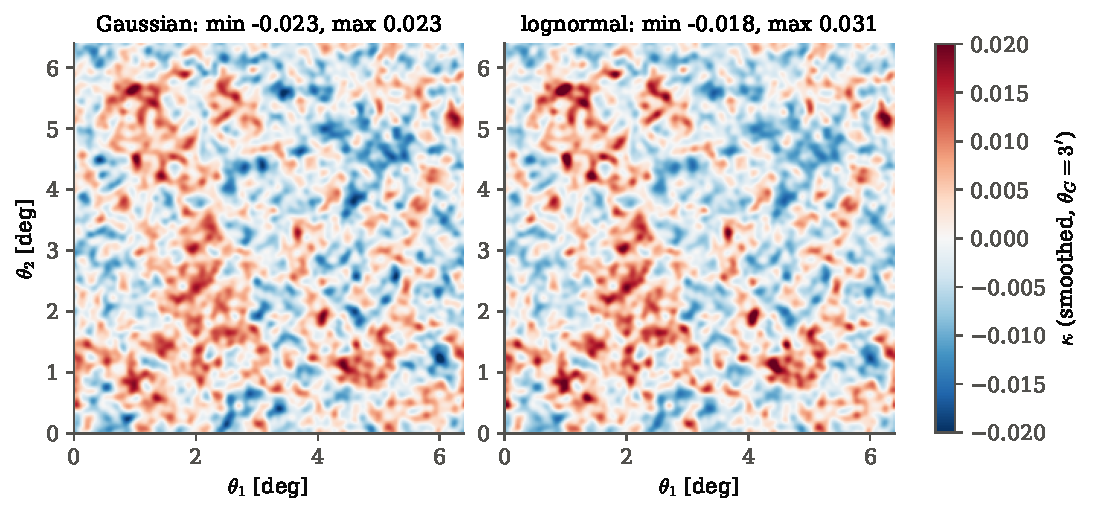
\includegraphics[width=\linewidth]{figures/ch12/w_lognormal_maps.pdf}
\caption{A Gaussian convergence map (left) and a shifted lognormal one (right), built from the same white noise and
with the same power spectrum, both smoothed with a $3'$ Gaussian. The large-scale pattern is identical. The
lognormal map has compact, intense red spots, where many lenses line up, and shallow, wide blue regions, because
it cannot fall far below zero: compare the minimum and maximum in the titles.}
\label{12w:fig:ln-maps}
\end{figure}

\begin{figure}[htbp]
\centering
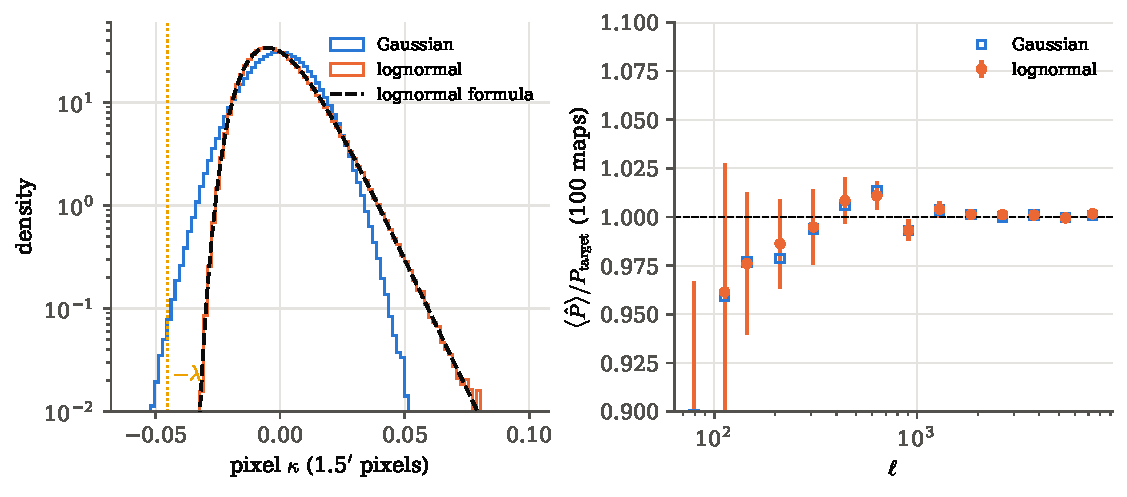
\includegraphics[width=\linewidth]{figures/ch12/w_lognormal_pdf.pdf}
\caption{Left: the distribution of pixel values in 20 Gaussian and 20 lognormal maps ($1.5'$ pixels, logarithmic
vertical axis), with the lognormal density obtained from \eqref{12w:eq:lognormal} by a change of variables (dashed).
The Gaussian is symmetric; the lognormal stops at the floor $-\lambda$ (dotted line) and has a long tail to high
$\kappa$. Right: the band powers of $100$ maps of each kind divided by the target spectrum. Both reproduce it; the
scatter at low $\ell$, the same for both since the maps share their white noise, is the sampling variance of the
few modes there.}
\label{12w:fig:ln-pdf}
\end{figure}

\paragraph{What the maps show.} Over $\WNsimOne$ maps, the measured skewness of the lognormal pixels is
$\WSkewLog$, against $\WSkewTheory$ from \eqref{12w:eq:ln-skew}; the Gaussian maps give $\WSkewGauss$. After
$3'$ smoothing the lognormal skewness is $\WSkewLogSm$ (the guide above said about $0.43$) and the Gaussian
$\WSkewGaussSm$. The lowest lognormal pixel in 20 maps is $\WMinLog$, inside the wall at $-\WLam$. The power spectrum
survives the transformation: for $\ell>300$ the mean band powers of the lognormal maps differ from the target by at
most $\WPowDev\%$; including the lowest bands the largest deviation is $\WPowDevLow\%$, the same as the Gaussian
maps' $\WPowDevG\%$, which is the sampling scatter of a handful of modes and not an error of the method
(\cref{12w:fig:ln-pdf}, right). So the two families of maps share their two-point statistics and differ in
everything else. That is exactly the situation in which a summary beyond $C_\ell$ can win.

\paragraph{What the lognormal model gets wrong.} It is a model of the one-point shape with one free number, and the
number we chose, the empty-beam shift, is not the best one. Xavier and collaborators made convergence maps the
honest way, as sums of correlated lognormal density slices along the line of sight, and asked which shift a
lognormal fitted to them needs. For sources at $z=2.1$ the empty-beam value is $0.2115$, while matching the
first three moments gives $0.1288$ \cite[Table~2]{Xavier2016}. The empty beam overestimates the shift by about
$60\%$, so by $S_3\approx3/\lambda$ it underestimates the skewness by a similar factor: our maps are less
non-Gaussian than the real sky, and any gain we find from non-Gaussian summaries is, if anything, too small. The
reason is physical: a real line of sight is never empty, and the deepest voids have $\delta\approx-0.8$, not $-1$.
A sum of lognormal slices is also not itself lognormal \cite[§3.3]{Xavier2016}, and a lognormal field has no
haloes, no filaments and no lensing of lensing. For each of these the research analyses use ray-traced $N$-body
maps \cite{Takahashi2017sims}; we return to the cost in \cref{12w:sec:research}.
\section{From galaxy shapes to a mass map}
\label{12w:sec:ks}

A survey never sees the convergence. It sees galaxies, each with a measured ellipticity
$\varepsilon\approx\varepsilon^{(0)}+\gamma$: its own random shape $\varepsilon^{(0)}$ plus the shear $\gamma$ of
\cref{T1b:sec:objects}, a spin-2 quantity, a headless stick. Peaks, islands and lakes are properties of a map
of $\kappa$, so before any of the summaries of \cref{12a:sec:excursion,12b:sec:filtration} can be computed, the
convergence must be reconstructed from the sticks. Three things stand between the sticks and the map. The
reconstruction itself is non-local: the shear at one point is caused by matter everywhere. The shapes carry noise
some thirty times larger than the signal (\cref{T1b:sec:noise}). And part of every survey is missing, behind bright
stars and beyond its edges.

\paragraph{The question.} Given the shear on a patch of sky, which convergence produced it? And how faithful is the
answer when each galaxy's shape is mostly its own, and when some of the patch is blank?

\subsection{The inversion, mode by mode}
\label{12w:sec:ks-chain}

Recall the two second-derivative relations of \cref{T1b:sec:objects}, in the flat angles $\theta_1,\theta_2$ of
\cref{T1b:fig:sky-plane}: the convergence is half the Laplacian of the lensing potential, $\kappa=\frac12(\psi_{,11}
+\psi_{,22})$, and the shear is $\gamma\equiv\gamma_1+i\gamma_2$ with $\gamma_1=\frac12(\psi_{,11}-\psi_{,22})$ and
$\gamma_2=\psi_{,12}$, a comma meaning a derivative. Both are linear in one unknown function, so we should eliminate
it. Derivatives become multiplications in Fourier space. Write each field on the patch as a sum of plane waves,
$f(\bm\theta)=\int\frac{\dd^2\ell}{(2\pi)^2}\hat f(\bm\ell)e^{i\bm\ell\cdot\bm\theta}$, with
$\bm\ell=(\ell_1,\ell_2)=\ell(\cos\varphi_\ell,\sin\varphi_\ell)$, so that $\partial/\partial\theta_a$ acting on a
wave multiplies it by $i\ell_a$. Then, for every $\bm\ell\neq\bm0$,
\begin{align}
\hat\kappa
&\eqby{1}\tfrac12\bigl[(i\ell_1)^2+(i\ell_2)^2\bigr]\hat\psi=-\tfrac12\ell^2\hat\psi,
\nonumber\\
\hat\gamma\equiv\hat\gamma_1+i\hat\gamma_2
&\eqby{2}\tfrac12\bigl[(i\ell_1)^2-(i\ell_2)^2\bigr]\hat\psi+i\,(i\ell_1)(i\ell_2)\hat\psi
=-\tfrac12\bigl(\ell_1^2-\ell_2^2+2i\ell_1\ell_2\bigr)\hat\psi
\nonumber\\
&\eqby{3}-\tfrac12(\ell_1+i\ell_2)^2\hat\psi
\eqby{4}-\tfrac12\ell^2e^{2i\varphi_\ell}\hat\psi
\eqby{5}e^{2i\varphi_\ell}\,\hat\kappa ,
\label{12w:eq:ks-forward}\\
\hat\kappa&\eqby{6}e^{-2i\varphi_\ell}\,\hat\gamma .
\label{12w:eq:ks}
\end{align}
\begin{explain}
  \item The Laplacian of a plane wave: each derivative brings down $i\ell_a$, and $i^2=-1$.
  \item The two shear components with the same rule, combined into one complex number.
  \item $(\ell_1+i\ell_2)^2=\ell_1^2-\ell_2^2+2i\ell_1\ell_2$.
  \item $\ell_1+i\ell_2=\ell e^{i\varphi_\ell}$, the polar form of the wavevector.
  \item The first line: $-\frac12\ell^2\hat\psi=\hat\kappa$.
  \item Multiply both sides by $e^{-2i\varphi_\ell}$, which has modulus one.
\end{explain}
\Cref{12w:eq:ks} is the \newterm{Kaiser--Squires inversion} \cite{KaiserSquires1993}. In the notation of
\srcref{BartelmannSchneider2001}{p.~88, eqs.~5.2--5.3} it reads $\hat\kappa=\pi^{-1}\hat{\mathcal D}^*\hat\gamma$ with
$\hat{\mathcal D}=\pi e^{2i\varphi_\ell}$, the row of the table in \cref{T1b:sec:objects}. In words: a convergence
wave of any orientation produces a shear wave of the same wavelength whose sticks are turned by twice the angle of
the wavevector, and undoing the turn returns the convergence. Nothing is lost in either direction, because a
phase has modulus one.

Two remarks complete the inversion. First, the chain needs $\bm\ell\neq\bm0$: a uniform convergence $\kappa_0$
comes from $\psi=\frac12\kappa_0\theta^2$, whose $\psi_{,11}=\psi_{,22}$ and $\psi_{,12}=0$, so it makes no shear
at all. The map is therefore known only up to an added constant, the \newterm{mass-sheet degeneracy}
\srcref{BartelmannSchneider2001}{p.~88}. On a periodic simulated patch we fix the constant by requiring zero mean;
a peak height or a threshold measured from the mean is unaffected by it. Second, in real space the multiplication
by $e^{-2i\varphi_\ell}$ is a convolution with a kernel that falls only as $1/\theta^2$
\srcref{BartelmannSchneider2001}{eq.~5.4}: the convergence at a point is a weighted sum of the shear over the whole
patch. This is why a hole in the data will spoil the map well beyond its edge.

\paragraph{$E$ and $B$ from any stick field.}
Apply \eqref{12w:eq:ks} to a stick field that did \emph{not} come from a convergence, such as one with noise or an
error in it. The result is a complex map, and we name its two parts:
\begin{equation}
\kappa_E(\bm\theta)+i\kappa_B(\bm\theta)\equiv\int\!\frac{\dd^2\ell}{(2\pi)^2}\,e^{-2i\varphi_\ell}\,
\hat\gamma(\bm\ell)\,e^{i\bm\ell\cdot\bm\theta}.
\label{12w:eq:eb}
\end{equation}
If the sticks came from a real convergence, the integrand is $\hat\kappa(\bm\ell)$, whose inverse transform is the
real map $\kappa$, so $\kappa_E=\kappa$ and $\kappa_B=0$: lensing makes no $B$, the statement proved in real space
in \eqref{T1b:eq:no-b}. Now turn every stick by $45^\circ$. A stick at angle $\phi$ is $\abs\gamma e^{2i\phi}$, so the
turn multiplies $\gamma$ by $e^{2i\pi/4}=i$, and by linearity the output becomes $i\kappa$: the same map, moved
entirely into $\kappa_B$. This is the swirl pattern of \cref{T1b:fig:kappa-gamma}(b). Pure $E$ and pure $B$ are the
two ways a stick field can be arranged around each point, and \eqref{12w:eq:eb} sorts any field into them.

\pyfile[firstline=148,lastline=157,firstnumber=148]{code/ch12/lib_wl.py}{Shear from convergence and back}

The two functions are \eqref{12w:eq:ks-forward} and \eqref{12w:eq:eb} on the FFT grid: \pyname{E2IPHI} is the array
$e^{2i\varphi_\ell}=(\ell_1+i\ell_2)^2/\ell^2$ (step 3 of the chain, which avoids computing any angle), set to zero
at $\bm\ell=\bm0$, where the mass sheet lives. Lines~150 and 156 multiply every mode by the phase or its conjugate.

\paragraph{Example: the round trip.} Take one lognormal map of \cref{12w:sec:lognormal}, make its shear, and
invert. \pyname{w02_ks.py} finds that the recovered $\kappa_E$ differs from the input by at most $\WRoundE$ of the
map's rms, and $\kappa_B$ is at most $\WRoundB$ of it: zero to the precision of double arithmetic. The input map has
rms $\WKapRms$ and each shear component $\WGamRms$. Why smaller by $\sqrt2$? Because a phase of modulus one keeps
the power of every mode, the complex shear has the variance of $\kappa$, $\langle\abs\gamma^2\rangle=\langle
\gamma_1^2\rangle+\langle\gamma_2^2\rangle=\sigma_\kappa^2$, and on an isotropic sky the two components share it
equally: $\sigma_{\gamma_1}=\sigma_\kappa/\sqrt2=\WKapRms/1.414=0.0091$.

\subsection{Shape noise in the mass map}
\label{12w:sec:ks-noise}

Recall the noise of \eqref{T1b:eq:shape-noise}. With $\sigma_e=0.27$ the rms of one ellipticity component and
$\bar n$ galaxies per unit solid angle, a pixel of solid angle $A$ holds about $\bar nA$ galaxies and its mean
ellipticity scatters by $\sigma_e/\sqrt{\bar nA}$ in each component, independently from pixel to pixel. For the
KiDS-like density $\bar n=6.2\,\mathrm{arcmin}^{-2}$ and our $1.5'$ pixels this is
$0.27/\sqrt{6.2\times2.25}=\WSigPixNoise$ per component, against a signal of $\WGamRms$: the per-pixel
signal-to-noise ratio is about $1/8$. The inversion keeps the power of every mode, so the noise power
$\sigma_e^2/\bar n$ of each component goes, unchanged in total, into $\kappa_E$ and $\kappa_B$, each receiving
$\sigma_e^2/\bar n$; fifty pure-noise maps give $\WNoiseRatioE$ and $\WNoiseRatioB$ times $\sigma_e^2/\bar n=
\WNoisePow$ in $E$ and $B$. The noise is white, the same at every $\ell$, while the signal falls with $\ell$; at
the pixel scale the map is all noise. Shrinking the pixels makes it worse without limit, the ``infinite noise'' of
a direct inversion \srcref{BartelmannSchneider2001}{p.~88}. The cure is to smooth.

\emph{How much noise survives smoothing?} Smooth with a normalised Gaussian of standard deviation $\theta_G$,
$W(\bm\theta)=e^{-\theta^2/2\theta_G^2}/(2\pi\theta_G^2)$. White noise $n(\bm\theta)$ with power $N$ has the
correlation $\langle n(\bm\theta)n(\bm\theta')\rangle=N\,\delta^{(2)}(\bm\theta-\bm\theta')$ (a field of independent
pixels, \cref{T1b:sec:objects}). The smoothed noise is $n_s(\bm\theta)=\int\dd^2\theta'\,W(\bm\theta-\bm\theta')
n(\bm\theta')$, so
\begin{align}
\sigma_{\rm noise}^2\equiv\langle n_s^2\rangle
&\eqby{1}\int\!\dd^2\theta_1\!\int\!\dd^2\theta_2\,W(\bm\theta-\bm\theta_1)W(\bm\theta-\bm\theta_2)\,
N\delta^{(2)}(\bm\theta_1-\bm\theta_2)
\eqby{2}N\!\int\!\dd^2\theta'\,W^2(\bm\theta')
\nonumber\\
&\eqby{3}\frac{N}{(2\pi\theta_G^2)^2}\int_0^\infty\!2\pi\vartheta\,e^{-\vartheta^2/\theta_G^2}\,\dd\vartheta
\eqby{4}\frac{N}{4\pi^2\theta_G^4}\,\pi\theta_G^2
\eqby{5}\frac{\sigma_e^2}{4\pi\theta_G^2\,\bar n}.
\label{12w:eq:sigma-noise}
\end{align}
\begin{explain}
  \item Square the smoothed noise and average; only the noise is random.
  \item The delta function removes one integral; shift the variable.
  \item Insert $W^2$ and use polar coordinates.
  \item $\int_0^\infty2\pi\vartheta e^{-\vartheta^2/\theta_G^2}\dd\vartheta=\pi\theta_G^2$ (substitute $u=\vartheta^2$).
  \item $N=\sigma_e^2/\bar n$ for $\kappa_E$.
\end{explain}
The smoothing area $4\pi\theta_G^2$ counts the galaxies that the filter effectively averages. For $\theta_G=3'$
and $\bar n=6.2\,\mathrm{arcmin}^{-2}$, $\sigma_{\rm noise}^2=0.0729/(4\pi\times9\times6.2)=1.04\times10^{-4}$, so
$\sigma_{\rm noise}=\WSigNCont$. On the pixel grid the same quantity is a lattice sum over the modes, and it gives
$\WSigNLat$; fifty noise maps give $\WSigNMeas$. The smoothed signal has rms $\WSigSm$
(\cref{12w:sec:maps-code}), so even after smoothing each pixel is dominated by noise. Every peak, island and lake of
the mass map will be measured in units of this $\sigma_{\rm noise}$, the signal-to-noise map
$\nu(\bm\theta)\equiv\kappa_{E,s}(\bm\theta)/\sigma_{\rm noise}$.

\paragraph{Example: a published noise level, recovered.}
Kratochvil and collaborators quote the smoothed noise as $\sigma_{\rm noise}^2=\langle\sigma_\gamma^2\rangle/
(2\pi\theta_G^2n_{\rm gal})$ \cite[eq.~9]{Kratochvil2010}, with $\sigma_\gamma$ the rms of one shear component.
Compared with \eqref{12w:eq:sigma-noise} the $4\pi$ has become $2\pi$. The two agree if their $\theta_G$ is the
width in $e^{-\theta^2/\theta_G^2}$, a standard deviation of $\theta_G/\sqrt2$: then $4\pi(\theta_G/\sqrt2)^2=
2\pi\theta_G^2$. Their own numbers confirm this reading. With $\sigma_\gamma=0.15+0.035z=0.22$ for sources at
$z=2$, $n_{\rm gal}=15\,\mathrm{arcmin}^{-2}$ and $\theta_G=1'$, the formula gives $\sigma_{\rm noise}^2=0.0484/
(2\pi\times15)=5.1\times10^{-4}$, $\sigma_{\rm noise}=0.0227$, and their detection threshold of $4.5\sigma_{\rm
noise}$ is $0.102$, the value they quote. A smoothing scale is a number with a convention attached, like the
$\sigma_e$ of \cref{T1b:sec:conventions}.

\subsection{Aperture mass: a filtered map without the inversion}
\label{12w:sec:aperture}

Kaiser--Squires builds the convergence at a point from the shear of the whole patch, and then we smooth it. The
peak analyses of Dietrich and Hartlap and of Heydenreich and collaborators do not do it in two steps. They compute the
\newterm{aperture mass}, a filtered convergence obtained straight from the sticks \cite{DietrichHartlap2010,
Heydenreich2021}. \emph{Can the filter be put inside the inversion?} Choose a round filter $U(\abs{\bm\theta})$ and
ask for
\begin{equation}
M(\bm\theta_0)\equiv\int\!\dd^2\theta\,U(\abs{\bm\theta-\bm\theta_0})\,\kappa(\bm\theta),
\qquad\int\!\dd^2\theta\,U=0,
\label{12w:eq:map-def}
\end{equation}
the convergence averaged around $\bm\theta_0$ with weight $U$. The second condition makes the filter
\newterm{compensated}: positive in the middle and negative in a ring, so that its total weight is zero. We express
$M$ through the shear. The convolution theorem turns \eqref{12w:eq:map-def} into a sum over modes, and
\eqref{12w:eq:ks} replaces $\hat\kappa$:
\begin{align}
M(\bm\theta_0)
&\eqby{1}\int\!\frac{\dd^2\ell}{(2\pi)^2}\,\hat U(\ell)\,\hat\kappa(\bm\ell)\,e^{i\bm\ell\cdot\bm\theta_0}
\eqby{2}\int\!\dd^2\theta\,\gamma(\bm\theta)\,K(\bm\theta_0-\bm\theta),
\nonumber\\
K(\bm x)
&\equiv\int\!\frac{\dd^2\ell}{(2\pi)^2}\,\hat U(\ell)\,e^{-2i\varphi_\ell}\,e^{i\bm\ell\cdot\bm x}
\nonumber\\
&\eqby{3}\int_0^\infty\!\frac{\ell\,\dd\ell}{(2\pi)^2}\,\hat U(\ell)\int_0^{2\pi}\!\dd\varphi_\ell\,
e^{-2i\varphi_\ell}\,e^{i\ell\abs{\bm x}\cos(\varphi_\ell-\varphi_x)}
\nonumber\\
&\eqby{4}-e^{-2i\varphi_x}\,Q(\abs{\bm x}),
\qquad Q(\vartheta)\equiv\int_0^\infty\!\frac{\ell\,\dd\ell}{2\pi}\,\hat U(\ell)\,J_2(\ell\vartheta).
\label{12w:eq:map-chain}
\end{align}
\begin{explain}
  \item The transform of a filtered map is the product of the transforms ($U$ is even, so $\hat U$ is real and
        depends on $\ell$ only).
  \item Insert $\hat\kappa=e^{-2i\varphi_\ell}\hat\gamma$ and write $\hat\gamma(\bm\ell)=\int\dd^2\theta\,\gamma(\bm\theta)
        e^{-i\bm\ell\cdot\bm\theta}$; the $\bm\ell$ integral moves inside and collects into the kernel $K$.
  \item Polar coordinates in $\bm\ell$, with $\varphi_x$ the polar angle of $\bm x$, so that $\bm\ell\cdot\bm x=
        \ell\abs{\bm x}\cos(\varphi_\ell-\varphi_x)$.
  \item Shift the angle, $\varphi_\ell=\varphi_x+\alpha$, which pulls out $e^{-2i\varphi_x}$, and use the Bessel
        integral $\int_0^{2\pi}e^{-2i\alpha}e^{iz\cos\alpha}\dd\alpha=2\pi\,i^{-2}J_{-2}(z)=-2\pi J_2(z)$.
\end{explain}
For a map that is pure $E$ the result is real, so we may keep the real part. With $\bm x=\bm\theta_0-\bm\theta$ the angle
$\varphi_x$ differs from the polar angle $\varphi$ of $\bm\theta-\bm\theta_0$ by $\pi$, which leaves $e^{-2i\varphi_x}=
e^{-2i\varphi}$, and
\begin{equation}
M(\bm\theta_0)=\int\!\dd^2\theta\,Q(\abs{\bm\theta-\bm\theta_0})\,\gamma_t(\bm\theta;\bm\theta_0),
\qquad\gamma_t(\bm\theta;\bm\theta_0)\equiv-\mathrm{Re}\bigl[\gamma(\bm\theta)\,e^{-2i\varphi}\bigr].
\label{12w:eq:map-gt}
\end{equation}
The number $\gamma_t$ is the \newterm{tangential shear}: the component of the stick at $\bm\theta$ along the direction
that circles $\bm\theta_0$. For a stick tangential to the circle, $\gamma=-\abs\gamma e^{2i\varphi}$ (the pattern
around a lump found in \cref{T1b:sec:objects}), so $\gamma_t=+\abs\gamma$; a radial stick gives $-\abs\gamma$. The
real-space form of the weight, $Q(\vartheta)=(2/\vartheta^2)\int_0^\vartheta\vartheta'U(\vartheta')\dd\vartheta'-
U(\vartheta)$, is the one quoted by \cite[eq.~2]{Heydenreich2021}; the Bessel form above is what falls out of our
inversion. Three things follow at once.
\emph{No mass sheet.} The compensation condition says $\hat U(0)=\int U\,\dd^2\theta=0$. A constant $\kappa_0$ lives
only in the mode $\bm\ell=\bm0$, which $\hat U$ removes, so $M$ is blind to it: the degeneracy of
\cref{12w:sec:ks-chain} is built out of the observable.
\emph{Holes cost only what they hold.} \Cref{12w:eq:map-gt} is an integral over the sticks that exist. In the estimator
below a masked galaxy is a term missing from a sum, and the aperture around a hole is merely less well measured,
whereas a Kaiser--Squires map is spoiled over the whole range of its $1/\theta^2$ kernel
(\cref{12w:sec:ks-mask}). Heydenreich and collaborators discard the pixels for which at least half the aperture is
masked \cite[§2.2]{Heydenreich2021}.
\emph{A noise level.} Replace the integral by a sum over the $\bar n$ galaxies per unit solid angle, each carrying its
measured ellipticity $\varepsilon_{t,i}=\varepsilon^{(0)}_{t,i}+\gamma_t$: $\hat M=\bar n^{-1}\sum_iQ_i\,\varepsilon_{t,i}$.
The intrinsic tangential components are independent with variance $\sigma_e^2$, so
\begin{equation}
\sigma_M^2\ \eqby{1}\ \frac{1}{\bar n^2}\,\bar n\!\int\!\dd^2\theta\,Q^2\,\sigma_e^2
\ \eqby{2}\ \frac{\sigma_e^2}{\bar n}\int\!\dd^2\theta\,Q^2(\abs{\bm\theta}) .
\label{12w:eq:map-noise}
\end{equation}
\begin{explain}
  \item The variance of a sum of independent terms is the sum of the variances, and the number of galaxies in
        $\dd^2\theta$ is $\bar n\,\dd^2\theta$.
  \item Collect the constants.
\end{explain}
This is the shape of \eqref{12w:eq:sigma-noise}, in which the Gaussian $W$ played the part of $Q$: smoothed noise is
always $\sigma_e^2/\bar n$ times the integral of the square of the weight. The aperture-mass \newterm{signal-to-noise
map} is $\nu=M/\sigma_M$, and it is the map of the three published analyses; Heydenreich and collaborators choose $Q$
as a smooth function shaped like the lensing signal of a typical dark-matter halo, so that the peaks of $\nu$ are
tuned to haloes \cite[§2.2.1]{Heydenreich2021}. We use the Gaussian-smoothed Kaiser--Squires map, which is
easier to simulate on a periodic grid and has the same noise algebra. The two maps are two different linear filters of
the same shear, so the qualitative behaviour of their peaks and islands, which is what the comparisons of
\cref{12w:sec:beyond-repro} rest on, is the same, and the numbers are not.

\subsection{What a mask does to the map}
\label{12w:sec:ks-mask}

Real data have holes. Our mask removes $40$ discs of radius $3'$ to $9'$ around imagined bright stars and a strip of
$0.4^\circ$ along one edge, keeping a fraction $f_{\rm obs}=\WFobs$ of the patch. Where there is no galaxy, the
measured shear is zero. What does \eqref{12w:eq:eb} do with a shear map that is suddenly zero inside a hole?

A masked shear map is not the shear of any convergence. Inside a hole the true $\kappa$ is not zero, yet the sticks
around it are gone, and the inversion, which builds $\kappa$ at a point from the sticks everywhere with a $1/\theta^2$
kernel, attributes the missing pattern partly to a different convergence and partly to $B$. In Fourier language the
mask multiplies the shear by a window $W(\bm\theta)$, which convolves its transform: the mode $\bm\ell$ of the
masked shear is a mixture of modes $\bm\ell'$ of the true one, each carrying the phase $e^{2i\varphi_{\ell'}}$ of its
own wavevector. Undoing it with the phase $e^{-2i\varphi_\ell}$ of the new wavevector leaves the factor
$e^{2i(\varphi_{\ell'}-\varphi_\ell)}$, whose imaginary part feeds $B$. The equation is derived in \cref{12w:sec:pcl}. The effect should be strongest next to a hole, where the missing sticks are close, and fade with
distance.

\begin{figure}[htbp]
\centering
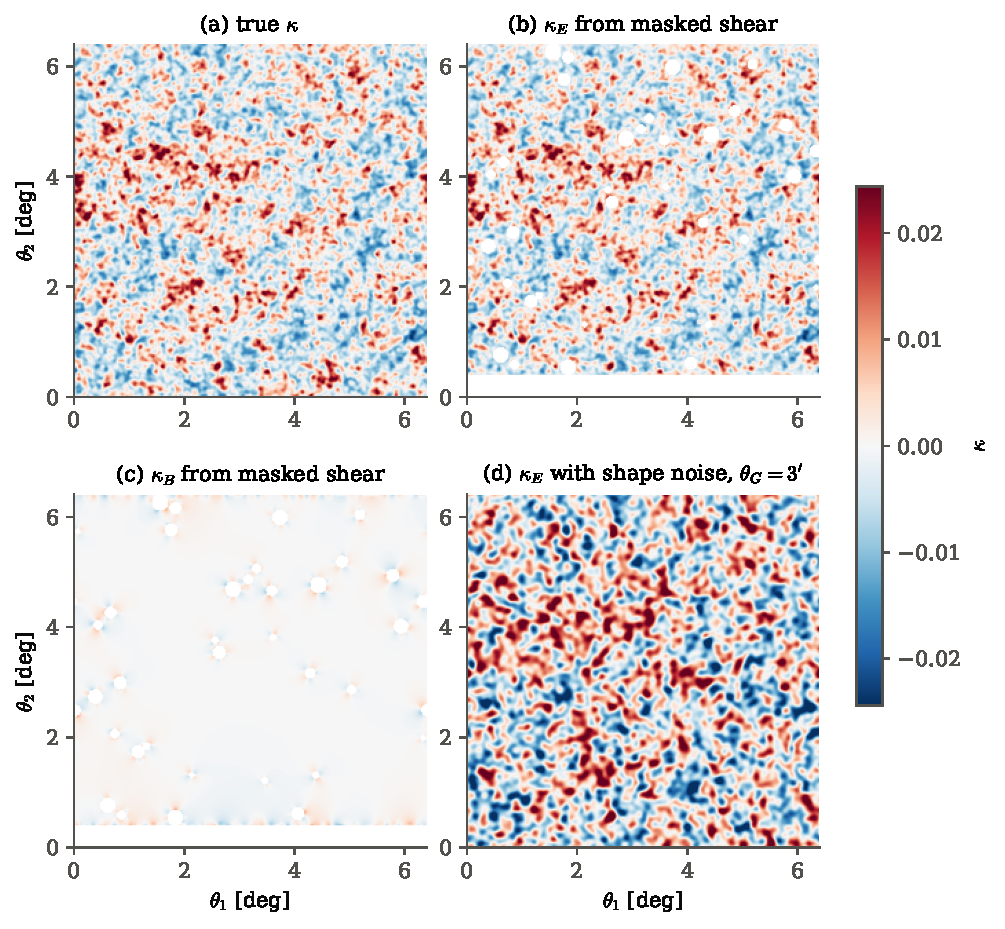
\includegraphics[width=0.92\linewidth]{figures/ch12/w_ks_maps.pdf}
\caption{(a) A lognormal convergence map ($1.5'$ smoothing for display). (b) The $E$ map reconstructed from its
shear with the mask applied: away from the holes and the edge strip (grey) it is the map of panel (a). (c) The $B$
map of the same masked shear: zero far from the mask, rings around every hole. (d) The $E$ map from the full,
unmasked shear with KiDS-like shape noise, smoothed with $\theta_G=3'$: the strongest peaks of panel (a) survive,
the rest of the structure is mixed with noise.}
\label{12w:fig:ks-maps}
\end{figure}

\Cref{12w:fig:ks-maps} shows it, and the numbers confirm it. Within $3'$ of a masked pixel the error of $\kappa_E$
has an rms of $\WErrNear$ times the rms of the map, and $\kappa_B$ has $\WBNear$ of it; farther than $30'$ from any
masked pixel the two fall to $\WErrFar$ and $\WBFar$. In power, the masked $B$ map carries $\WLeakLow\%$ of the $E$
power at the lowest band ($\ell\approx200$) and $\WLeakHigh\%$ at the highest ($\ell\approx5000$), and the $E$ power
is lowered to $\WSuppLow$ and $\WSuppHigh$ of its true value, against an observed fraction $f_{\rm obs}$ of the area: most of the loss is simply the
missing area. For the topological summaries the lesson is local: features near holes are unreliable, and a
research analysis either excludes a margin around the mask or, better, applies the same mask to every simulation, so
that the distortion is part of the model; Heydenreich and collaborators handle masked pixels with relative homology
for the same reason \cite[§2.3.3]{Heydenreich2021}. We sidestep the problem for the summaries of
\cref{12w:sec:beyond} by analysing full periodic patches, and keep the mask for the power spectrum, where
\cref{12w:sec:pcl} shows how to undo it.

\subsection{Reproducing a published test: how much to smooth a mass map}
\label{12w:sec:jeffrey}

\paragraph{Their question.} The Dark Energy Survey published mass maps of its Year~3 footprint, $4143\,\mathrm{deg}^2$
of sky. Jeffrey, Gatti and collaborators asked which reconstruction method, and which amount of smoothing, gives
the map closest to the truth \cite{Jeffrey2021DESmass}. The answer matters for anyone who wants to count peaks or
voids in the map: too little smoothing and the map is noise; too much and the structures are washed out.

\paragraph{Their setup.} A full-sky ray-traced convergence map of \cite{Takahashi2017sims} played the true sky. They
placed the DES Y3 galaxies on it, with the real positions, footprint and weights, $n_{\rm eff}=5.59$ galaxies per
square arcminute, and shape noise drawn by rotating the real ellipticities at random. They reconstructed $\kappa_E$
by Kaiser--Squires on the sphere at HEALPix $N_{\rm side}=1024$ ($3.44'$ pixels), and by three methods with priors,
and smoothed the Kaiser--Squires map with Gaussians of standard deviation $\theta$ from $0$ to $40'$.

\paragraph{Their key equation.} Their inversion is \eqref{12w:eq:ks}; their eq.~(22) is its flat-sky form. Their
score is the \newterm{Pearson correlation coefficient} between the true map $\kappa$ and the reconstruction
$\hat\kappa$ \cite[eq.~35]{Jeffrey2021DESmass}, the correlation coefficient of \cref{ch:01} computed over pixels,
$r=\langle\kappa\hat\kappa\rangle/\sqrt{\langle\kappa^2\rangle\langle\hat\kappa^2\rangle}$ (both maps with zero
mean). Why should $r$ have a maximum as $\theta$ grows? Write the smoothed reconstruction mode by mode as
$\hat\kappa_{\bm\ell}=W_\ell(\kappa_{\bm\ell}+n_{\bm\ell})$, with $W_\ell$ the transform of the smoothing kernel
($e^{-\ell^2\theta^2/2}$ for a Gaussian), $C_\ell$ the signal power and $N$ the noise power. Different modes are
uncorrelated, and the noise is uncorrelated with the signal, so each average is a sum over modes:
\begin{align}
r
&\eqby{1}\frac{\sum_{\bm\ell}W_\ell C_\ell}{\sqrt{\sum_{\bm\ell}C_\ell}\,\sqrt{\sum_{\bm\ell}W_\ell^2(C_\ell+N)}}
\eqby{2}\frac{\sum_{\bm\ell}a_\ell b_\ell}{\sqrt{\sum_{\bm\ell}C_\ell}\,\sqrt{\sum_{\bm\ell}a_\ell^2}}
\relby{3}{\le}\Bigl[\frac{\sum_{\bm\ell}C_\ell^2/(C_\ell+N)}{\sum_{\bm\ell}C_\ell}\Bigr]^{1/2},
\label{12w:eq:pearson}
\end{align}
\begin{explain}
  \item Parseval's theorem turns each pixel average into a sum over modes: $\langle\kappa\hat\kappa\rangle$ picks up
        $W_\ell C_\ell$ from each mode, $\langle\hat\kappa^2\rangle$ picks up $W_\ell^2(C_\ell+N)$.
  \item Name $a_\ell\equiv W_\ell\sqrt{C_\ell+N}$ and $b_\ell\equiv C_\ell/\sqrt{C_\ell+N}$, so that $a_\ell b_\ell=
        W_\ell C_\ell$.
  \item The Cauchy--Schwarz inequality, $\sum ab\le\sqrt{\sum a^2}\sqrt{\sum b^2}$, with equality when $a_\ell\propto b_\ell$.
\end{explain}
The bound is reached when $W_\ell\propto C_\ell/(C_\ell+N)$: pass a mode in proportion to the fraction of its power
that is signal. That filter is the Wiener filter, which is why the Wiener reconstruction of Jeffrey and collaborators
beats every smoothed Kaiser--Squires map in their Fig.~6. A Gaussian $W_\ell$ can only imitate it: it passes
everything below $\ell\sim1/\theta$ and nothing above. If $\theta$ is too small, it passes noise-dominated modes,
which add to the denominator only; if too large, it removes signal-dominated modes from the numerator. The best
$\theta$ puts the cut near the multipole where $C_\ell=N$, which moves to higher $\ell$, so to smaller $\theta$, as
the galaxy density grows. That is the prediction to test.

\paragraph{What we compute.} \pyname{w02_ks.py} makes 20 lognormal maps, adds the shape noise of three surveys (DES
Y3, $n=5.59$, $\sigma_e=0.268$; our KiDS-like $6.2$ and $0.27$; a Stage-IV-like $30$ and $0.27$), inverts, smooths
with $\theta$ from $0.75'$ to $20'$, and computes $r$ against the true map at our $1.5'$ resolution and against the
true map smoothed to the size of an $N_{\rm side}=1024$ pixel, which is what they compared with.

\pyfile[firstline=128,lastline=140,firstnumber=128]{code/ch12/w02_ks.py}{The Pearson test}

\begin{figure}[htbp]
\centering
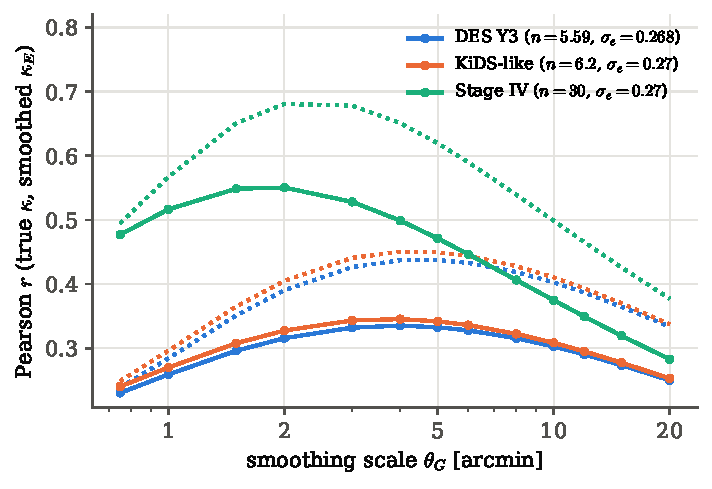
\includegraphics[width=0.75\linewidth]{figures/ch12/w_ks_pearson.pdf}
\caption{Pearson correlation between the true convergence and the smoothed Kaiser--Squires map, as a function of the
smoothing scale, for three galaxy densities (solid: truth at our $1.5'$ pixels; dotted: truth averaged to the size of
a $N_{\rm side}=1024$ pixel, as in the DES Y3 test). Each curve rises while smoothing removes noise faster than signal
and falls once it removes signal; the optimum moves to smaller scales as the galaxy density grows.}
\label{12w:fig:ks-pearson}
\end{figure}

\paragraph{Side by side.} \Cref{12w:fig:ks-pearson} has the predicted shape. For the DES-like density our curve peaks
at $\theta=\WBestDES'$ with $r=\WBestRDES$; against the pixel-averaged truth at $\WBestDEShp'$ with $r=\WBestRDEShp$.
The KiDS-like case peaks at $\WBestKiDS'$ ($r=\WBestRKiDS$), and the Stage-IV case at $\WBestSfour'$ ($r=\WBestRSfour$).
Jeffrey and collaborators find the Kaiser--Squires $r$ rising from $0.20$ unsmoothed to about $0.31$ at $10'$, nearly
flat between $5'$ and $15'$, and slowly falling beyond \cite[Fig.~6]{Jeffrey2021DESmass}.

\paragraph{Why they differ.} The shapes agree and the optimum lies in the same range, a few to ten arcminutes, with
ours at the small end and our $r$ a little higher. Three causes push in this direction. Their truth is a ray-traced
$N$-body map, more strongly non-Gaussian than our lognormal one, with more of its signal in compact peaks that
smoothing removes. Their footprint has edges and holes everywhere, and \cref{12w:sec:ks-mask} showed how a mask
lowers the agreement near them; our patch has none. And their effective density varies over the footprint with the
depth of the images, while ours is uniform. Their grid of smoothing scales ($0,5,10,15,\dots$) also cannot resolve a
maximum this flat to better than $5'$. The galaxy density moves the optimum as \eqref{12w:eq:pearson} predicts: from
$\WBestDES'$ at $n=5.59$ to $\WBestSfour'$ at $n=30$.

\paragraph{The lesson.} The best smoothing scale is not a property of the method but of the data: it is set by
where the signal stops beating the noise, and a mass map from a deeper survey deserves less smoothing. The summaries
of \cref{12w:sec:beyond} use $\theta_G=3'$, close to the optimum for our density.
\section{The two-point analysis: band powers, their errors, and the banana}
\label{12w:sec:twopoint}

Every lensing survey so far has drawn its headline number from a two-point statistic: KiDS-1000 from band powers
and related statistics, DES Year~3 from the correlation functions $\xi_\pm$, HSC from power spectra
(\cref{T1b:sec:s8-surveys}). Before asking what the peaks and the topology of the mass map can add, we need the
number they must beat, computed in the same setting as everything else: our KiDS-like galaxy density, our source
sample, our patches. That calls for three pieces, each met before on the CMB. The band powers must be measured on a
patch with holes, which is the pseudo-$C_\ell$ problem of \cref{8b:sec:pseudo}, now for a spin-2 field. Their
errors must be known, which is the covariance problem of \cref{8b:sec:nsims}. And the errors must be turned into
errors on $(\Omega_m,\sigma_8)$, which is the Fisher matrix of \cref{10a:sec:gauss}.

\paragraph{The question.} On a KiDS-like survey of $1000\,\mathrm{deg}^2$, can the convergence power spectrum be
measured without bias through a mask, and how well does it then measure $\Omega_m$, $\sigma_8$ and $S_8$?

\subsection{Band powers through a mask: \texorpdfstring{$E$}{E} leaks into \texorpdfstring{$B$}{B}}
\label{12w:sec:pcl}

Recall the pseudo-$C_\ell$ idea of \cref{8b:sec:pseudo}: the power spectrum of a masked map is not the true
spectrum, but its \emph{average} is a known linear combination of the true band powers, through a coupling matrix
that depends only on the mask; inverting that matrix (MASTER, \cref{8b:sec:master}) removes the bias. For a scalar
CMB map the coupling comes from the window alone. \Cref{12w:sec:ks-mask} found a second effect for shear: the
mask also moves power from $E$ to $B$. We now derive both at once, on the flat periodic patch.

\emph{The masked shear, mode by mode.} Let the true shear be pure $E$, $\hat\gamma(\bm\ell)=e^{2i\varphi_\ell}
\hat E(\bm\ell)$, where $\hat E$ is the transform of the real map $\kappa$ \eqref{12w:eq:ks-forward}. The mask
$W(\bm\theta)$, one where we see and zero where we do not, multiplies the shear, so its transform $\hat W$ convolves
it. On the grid, with $N_{\rm pix}$ pixels, the convolution is a sum over the grid modes $\bm\ell'$. Apply the
inversion \eqref{12w:eq:eb} to the masked shear, and call the result $X(\bm\ell)=\hat E_W(\bm\ell)+i\hat B_W(\bm\ell)$,
where $\hat E_W$ and $\hat B_W$ are the transforms of the two real maps $\kappa_E$ and $\kappa_B$ made from the masked
shear:
\begin{align}
X(\bm\ell)
&\eqby{1}e^{-2i\varphi_\ell}\frac1{N_{\rm pix}}\sum_{\bm\ell'}\hat W(\bm\ell-\bm\ell')\,e^{2i\varphi_{\ell'}}\hat E(\bm\ell')
=\frac1{N_{\rm pix}}\sum_{\bm\ell'}\hat W(\bm\ell-\bm\ell')\,e^{2i(\varphi_{\ell'}-\varphi_\ell)}\hat E(\bm\ell'),
\nonumber\\
\hat E_W(\bm\ell)
&\eqby{2}\tfrac12\bigl[X(\bm\ell)+X(-\bm\ell)^*\bigr]
\eqby{3}\frac1{N_{\rm pix}}\sum_{\bm\ell'}\hat W(\bm\ell-\bm\ell')\cos\bigl[2(\varphi_{\ell'}-\varphi_\ell)\bigr]\hat E(\bm\ell'),
\nonumber\\
\hat B_W(\bm\ell)
&\eqby{4}\tfrac1{2i}\bigl[X(\bm\ell)-X(-\bm\ell)^*\bigr]
=\frac1{N_{\rm pix}}\sum_{\bm\ell'}\hat W(\bm\ell-\bm\ell')\sin\bigl[2(\varphi_{\ell'}-\varphi_\ell)\bigr]\hat E(\bm\ell').
\label{12w:eq:masked-eb}
\end{align}
\begin{explain}
  \item The transform of a product is the convolution of the transforms (with the $1/N_{\rm pix}$ of the discrete
        transform); then multiply by the phase of the inversion.
  \item A real map has a transform with $\hat f(-\bm\ell)=\hat f(\bm\ell)^*$. $X$ is the transform of the complex map
        $\kappa_E+i\kappa_B$, and the transform of its real part is the average of $X(\bm\ell)$ and $X(-\bm\ell)^*$.
  \item In $X(-\bm\ell)^*$ rename $\bm\ell'\to-\bm\ell'$ and use $\hat W(-\bm q)^*=\hat W(\bm q)$ and
        $\hat E(-\bm\ell')^*=\hat E(\bm\ell')$ (both maps are real), and $\varphi_{-\ell}=\varphi_\ell+\pi$, which leaves
        $e^{2i\varphi}$ unchanged. It becomes the same sum with $e^{-2i(\varphi_{\ell'}-\varphi_\ell)}$, and
        $\frac12(e^{ix}+e^{-ix})=\cos x$.
  \item The imaginary part in the same way, with $\frac1{2i}(e^{ix}-e^{-ix})=\sin x$.
\end{explain}
Each true mode $\bm\ell'$ feeds the masked mode $\bm\ell$ with the window's weight $\hat W(\bm\ell-\bm\ell')$, split
between $E$ and $B$ by the angle between the two wavevectors. Without a mask $\hat W$ is a spike at zero, only
$\bm\ell'=\bm\ell$ contributes, the angle is zero, and everything stays in $E$. With a mask, nearby wavevectors at an
angle leak a fraction $\sin^2$ of their power into $B$.

\emph{The average power.} Different true modes are uncorrelated, $\langle\hat E(\bm\ell')\hat E(\bm\ell'')^*\rangle
=N_{\rm pix}A_{\rm pix}^{-1}C_{\ell'}\,\delta_{\bm\ell'\bm\ell''}$ on the grid \eqref{7a:eq:fft-target}. Squaring
\eqref{12w:eq:masked-eb} and averaging keeps only the diagonal terms:
\begin{equation}
\langle\tilde C^E_\ell\rangle=\sum_{\bm\ell'}w_2(\bm\ell-\bm\ell')\cos^2\bigl[2(\varphi_{\ell'}-\varphi_\ell)\bigr]C_{\ell'},
\qquad
\langle\tilde C^B_\ell\rangle=\sum_{\bm\ell'}w_2(\bm\ell-\bm\ell')\sin^2\bigl[2(\varphi_{\ell'}-\varphi_\ell)\bigr]C_{\ell'},
\label{12w:eq:coupling}
\end{equation}
with $w_2(\bm q)\equiv\abs{\hat W(\bm q)}^2/N_{\rm pix}^2$ the power of the window. Three checks. Without a mask
$w_2$ is one at $\bm q=\bm0$ and zero elsewhere, and \eqref{12w:eq:coupling} returns $C_\ell$ in $E$ and nothing in
$B$. By Parseval, $\sum_{\bm q}w_2(\bm q)=N_{\rm pix}^{-1}\sum_{\bm\theta}W^2=f_{\rm obs}$, the observed fraction,
so a flat spectrum $C_\ell=N$ put into both $E$ and $B$ (shape noise, \cref{12w:sec:ks-noise}) comes out as
$f_{\rm obs}N$ in each, whatever the angles, since $\cos^2+\sin^2=1$: the noise bias of a masked map is simply
$f_{\rm obs}N$. And the formula is the flat-sky version of the spin-2 coupling kernels of the MASTER family
\cite{Hivon2002}, the scalar case of \cref{8b:eq:M} with the cosine and sine as the only new ingredient. Binning
\eqref{12w:eq:coupling} into bands gives four matrices $M^{EE}_{bb'}$, $M^{BE}_{bb'}$ and, by the $45^\circ$
rotation of \cref{12w:sec:ks-chain}, $M^{BB}=M^{EE}$ and $M^{EB}=M^{BE}$; the decoupled band powers are the measured
pseudo band powers, noise subtracted, multiplied by the inverse of the $2\times2$ block matrix, as in
\eqref{8b:eq:bpw}.

\pyfile[firstline=60,lastline=84,firstnumber=60]{code/ch12/w03_twopoint.py}{The coupling matrices from the exact average}

\pyname{coupling_exact} evaluates \eqref{12w:eq:coupling} without a double sum over modes. The identity
$\cos^2x=\frac12(1+\cos2x)$ turns the $\cos^2[2\Delta\varphi]$ into $\frac12[1+\mathrm{Re}\,e^{4i(\varphi_{\ell'}-
\varphi_\ell)}]$, and each term is a convolution of $w_2$ with $C$ times a phase, done by FFT in line~70 (the
convolution theorem again, now used in reverse). Line~79 is the $e^{4i\varphi}$ term, lines~80--83 add or subtract the
two and average over each band. The bands are the eight analysis bands from $\ell=112$ to $5000$ plus one below
and one above, since power outside the analysed range also leaks into it. As a check the same matrices are measured
by brute force (\pyname{coupling}): $100$ Gaussian maps with power in one band at a time, masked, inverted, measured.
The diagonals agree to $\WMcDiag\%$, the Monte Carlo scatter of $100$ maps.

\paragraph{Example: what the coupling matrix says.} For our mask ($f_{\rm obs}=\WFobsT$) the largest off-diagonal
entry of $M^{EE}$, relative to the diagonal, is $\WOffDiag\%$, and the largest $E\to B$ entry is $\WLeakMax\%$ of the
diagonal: a mask of small holes couples neighbouring bands only weakly and leaks about one per cent of $E$ into $B$,
the same order as the $\WLeakLow\%$ to $\WLeakHigh\%$ found from the maps in \cref{12w:sec:ks-mask}.

\begin{figure}[htbp]
\centering
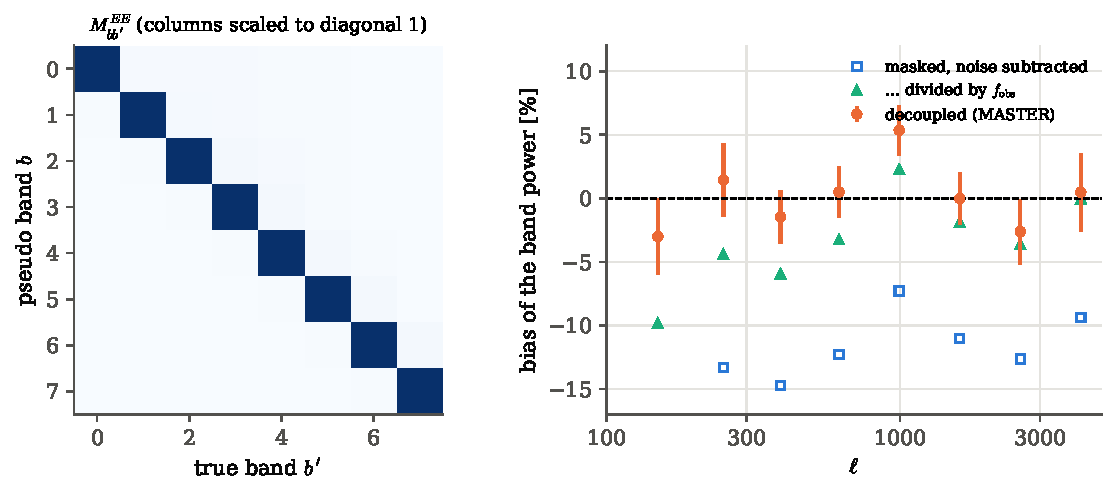
\includegraphics[width=\linewidth]{figures/ch12/w_pcl.pdf}
\caption{Left: the coupling matrix $M^{EE}$ of the masked patch, each column divided by its diagonal entry; it is
nearly diagonal. Right: the bias of the band powers over $200$ lognormal maps with KiDS-like shape noise. Masked and
noise-subtracted (squares): between $\WBiasRawMin\%$ and $\WBiasRawMax\%$, mostly the missing area. Divided by $f_{\rm obs}$ (triangles): up to
$\WBiasRescMax\%$, varying with $\ell$. Decoupled by the inverse coupling matrix (circles, with the Monte Carlo error of the
mean): consistent with zero.}
\label{12w:fig:pcl}
\end{figure}

\paragraph{Example: the recovered spectrum.} \pyname{w03_twopoint.py} makes $200$ lognormal maps with KiDS-like
noise, masks them and measures the band powers three ways (\cref{12w:fig:pcl}). The raw masked band powers, noise
subtracted, are $\WBiasRawMin\%$ to $\WBiasRawMax\%$ off. Dividing by $f_{\rm obs}$, the simplest correction, leaves
errors up to $\WBiasRescMax\%$. The decoupled band powers deviate by at most $\WBiasDecMax\%$ with a Monte Carlo error of
the mean up to $\WErrDecMax\%$; over the $\WNbands$ bands the $\chi^2$ of the mean against the truth is $\WChiE$.
The decoupled $B$ band powers give $\chi^2=\WChiB$ for $\WNbands$ degrees of freedom: consistent with zero, which is
the null test of \eqref{T1b:eq:no-b} passed on a masked map. The price of the mask is a scatter
$\WSdRatio$ times that of the unmasked patch, close to $1/\sqrt{f_{\rm obs}}=1.05$: fewer independent modes, as in
\cref{8a:sec:knox}.

\subsection{How large are the errors? Gaussian formula and simulations}
\label{12w:sec:cl-cov}

The Gaussian band-power error of \eqref{T1b:eq:band-error} assumes that each Fourier mode is a Gaussian variable.
On a flat patch of area $A$ it reads as follows. The grid modes form a lattice of spacing $2\pi/L$, with $L^2=A$, so a
ring of radius $\ell$ and width $\dd\ell$ holds $2\pi\ell\,\dd\ell/(2\pi/L)^2=\ell A\,\dd\ell/2\pi$ modes. The modes
come in pairs $\pm\bm\ell$ with the same power (the map is real), so a band of $n_b$ grid modes has $n_b/2$
independent ones. For a Gaussian mode the measured power $\abs{\hat\kappa}^2$ follows an exponential distribution,
whose standard deviation equals its mean $C_\ell+N$ (the $\chi^2_2$ of \eqref{7b:eq:chi2}, scaled). Averaging
$n_b/2$ independent such powers,
\begin{equation}
\Var\hat C_b=\frac{(C_b+N)^2}{n_b/2}=\frac{2(C_b+N)^2}{n_b},
\qquad n_b\simeq\frac{A}{2\pi}\int_{\rm band}\ell\,\dd\ell .
\label{12w:eq:flat-var}
\end{equation}
On the full sky $A=4\pi f_{\rm sky}$ and $n_b\simeq\int(2\ell+1)f_{\rm sky}\dd\ell$, which is \eqref{T1b:eq:band-error}
again: the same mode counting in a different coordinate system. Our bands hold from $\WModesLow$ grid modes (the
lowest) to $\WModesHigh$ (the highest).

A lognormal field is not Gaussian, and its band powers are not exponential sums: a single bright spot puts power in
many modes at once, so the modes are correlated and the variance is larger. \pyname{w05_costs.py} compares
\eqref{12w:eq:flat-var} with the scatter of the $\WNfidLN$ lognormal and $\WNfidG$ Gaussian fiducial maps of
\cref{12w:sec:beyond} (unmasked, with shape noise). For the Gaussian maps the ratio of the simulated to the
predicted variance lies between $\WCovRatioGmin$ and $\WCovRatioGmax$, within the Monte Carlo error of a variance
from $\WNfidG$ maps, $\sqrt{2/(n-1)}=\WCovRatioErrG$; the largest correlation between two bands is $\WCorrGmax$, also
noise. For the lognormal maps the ratio runs from $\WCovRatioLNmin$ to $\WCovRatioLNmax$, within their own error of
$\WCovRatioErrLN$, and no two bands are correlated by more than $\WCorrLNmax$, less than the noise correlation of the
Gaussian maps (\cref{12w:fig:cov-ratio}): in these maps the excess is too small to see. Shape noise is what rescues
the formula: where it dominates $C_b+N$, the noise, which is Gaussian and white, dilutes the non-Gaussian excess of
the signal.

\begin{figure}[htbp]
\centering
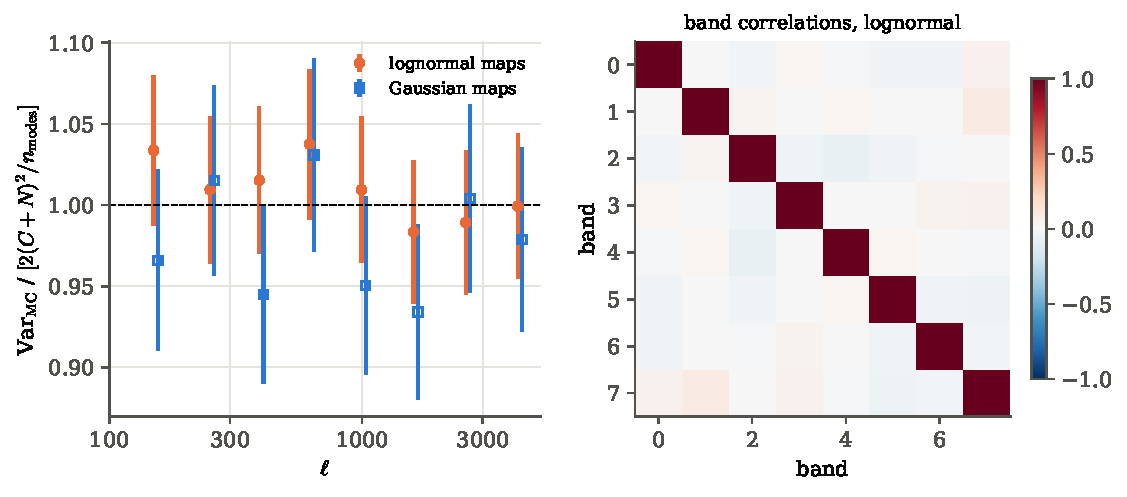
\includegraphics[width=\linewidth]{figures/ch12/w_cov_ratio.pdf}
\caption{Left: the variance of each band power over the simulated maps divided by the Gaussian prediction
\eqref{12w:eq:flat-var}, for lognormal and Gaussian maps with the same spectrum and the same shape noise. Right: the
correlation matrix of the eight band powers of the lognormal maps. Both sets of maps agree with the formula within
the Monte Carlo error, and the lognormal bands are no more correlated than noise allows: with this shape noise the
non-Gaussian excess stays below what $\WNfidLN$ maps can detect.}
\label{12w:fig:cov-ratio}
\end{figure}

This is the situation \cref{8b:sec:nsims} described for the CMB, now with a physical cause: the analytic covariance is
a good start, and simulations are needed for the part the analytic form leaves out. Research analyses add to the
Gaussian term a non-Gaussian term from the trispectrum and a \newterm{super-sample} term, the response of all modes to
density fluctuations larger than the survey, and check the sum against hundreds of simulations
\cite{Asgari2021KiDS,Takahashi2017sims}. Our forecast below uses the Gaussian formula, and \cref{12w:sec:beyond} uses
the simulated covariance throughout.

\subsection{From band powers to \texorpdfstring{$(\Omega_m,\sigma_8)$}{(Omega m, sigma 8)}: the Fisher forecast}
\label{12w:sec:cl-fisher}

Recall the Gaussian Fisher matrix \eqref{10a:eq:gauss-fisher}: for a data vector with mean $\bm\mu(\params)$ and a
covariance that does not depend on the parameters, $F_{ij}=\partial_i\bm\mu\T\Cmat^{-1}\partial_j\bm\mu$. With
independent bands, $\Cmat$ is diagonal with the variances \eqref{12w:eq:flat-var}, so
\begin{equation}
F_{ij}=\sum_b\frac{n_b}{2}\,\frac{\partial_iC_b\,\partial_jC_b}{(C_b+N)^2},
\qquad\params=(\Omega_m,\sigma_8),
\label{12w:eq:cl-fisher}
\end{equation}
the same expression as the signal-to-noise sum \eqref{T1b:eq:sn-one} with the derivative of the amplitude replaced
by the derivatives with respect to the parameters. The derivatives come from the Limber spectra at
$\Omega_m$ and $\sigma_8$ moved by $\pm5\%$, as central differences (\cref{10a:sec:numderiv}), and the survey is
$1000\,\mathrm{deg}^2$ with $n=6.2\,\mathrm{arcmin}^{-2}$ and $\sigma_e=0.27$ in one source bin.

\pyfile[firstline=87,lastline=100,firstnumber=87]{code/ch12/w03_twopoint.py}{The Gaussian band-power Fisher matrix}

Line~94 counts the modes per unit $\ell$ on the survey area, line~95 is the weight $n/2\,(C+N)^{-2}$, and the double
loop adds the products of derivatives.

\paragraph{The answer.} For $100\le\ell\le3000$ the marginal errors are $\sigma(\Omega_m)=\WSigOm$ and
$\sigma(\sigma_8)=\WSigSe$, with a correlation coefficient $r=\WRcorr$ between them, and the error on
$S_8$ is $\sigma(S_8)=\WSigSEight$, a precision of $\WSigSEightRel\%$. The individual errors are large and the
combination is small: the ellipse is a long needle along the valley of \cref{T1b:sec:s8}
(\cref{12w:fig:fisher-cl}). Had $\Omega_m$ been known, $\sigma_8$ would be measured to $\WSigSeFixed$; freeing it
inflates the error by the factor $1/\sqrt{1-r^2}=\WMargFactor$ of \eqref{T1b:eq:marg-cost}.

\paragraph{Example: why $S_8$ is not quite the needle.} The long axis of the ellipse, in the logarithms of the two
parameters, is the direction $\sigma_8\Omega_m^\alpha=$ const with $\alpha=\WAlphaF$, the exponent found multipole by
multipole in \cref{T1b:sec:s8-alpha} (there $0.57$ at $\ell=500$). The survey convention fixes $\alpha=0.5$. Write
\begin{align}
\ln S_8
&\eqby{1}\ln\sigma_8+0.5\ln\Omega_m+\text{const}
\eqby{2}\ln\bigl(\sigma_8\Omega_m^{\alpha}\bigr)-(\alpha-0.5)\ln\Omega_m+\text{const},
\nonumber\\
\sigma(\ln S_8)
&\relby{3}{\approx}\abs{\alpha-0.5}\,\sigma(\ln\Omega_m)
\approx0.08\times\frac{0.097}{0.315}\approx0.025 .
\label{12w:eq:s8-tilt}
\end{align}
\begin{explain}
  \item The definition $S_8=\sigma_8(\Omega_m/0.3)^{0.5}$.
  \item Add and subtract $\alpha\ln\Omega_m$.
  \item The first term is the best-measured combination, nearly fixed; the second inherits the large error of
        $\Omega_m$ along the needle.
\end{explain}
So $\sigma(S_8)\approx0.025\times0.83\approx0.021$, which is most of the $\WSigSEight$: the error on $S_8$ is set less
by the width of the needle than by the small tilt between the needle and the line of constant $S_8$. A survey that
quotes $\sigma_8\Omega_m^\alpha$ with its own $\alpha$, as HSC does with $\alpha=0.45$ \cite{Hikage2019HSC}, quotes the
narrowest number its data allow.

\paragraph{The banana.} The Fisher ellipse is the quadratic approximation of the log-likelihood at the fiducial
point (\cref{10a:sec:fisher}). Away from it the valley curves, because the constant-spectrum line is
$\sigma_8\propto\Omega_m^{-\alpha}$, a curve in the $(\Omega_m,\sigma_8)$ plane. \pyname{w03_twopoint.py} also
evaluates the Gaussian likelihood of the band powers on a $300\times300$ grid, with a power-law emulator
$C_b(\Omega_m,\sigma_8)=C_b^{\rm fid}(\sigma_8/\sigma_8^{\rm fid})^{a_b}(\Omega_m/\Omega_m^{\rm fid})^{b_b}$ built from the same
logarithmic derivatives. Its contours (\cref{12w:fig:fisher-cl}) follow the ellipse near the centre and bend into
the banana familiar from the published contours. From the grid, with a flat prior over the plotted box,
$\sigma(S_8)=\WSigSEightGrid$ and $\sigma(\Omega_m)=\WSigOmGrid$, close to the Fisher values: along $S_8$ the
likelihood is Gaussian, and the curvature only bends the long direction.

\begin{figure}[htbp]
\centering
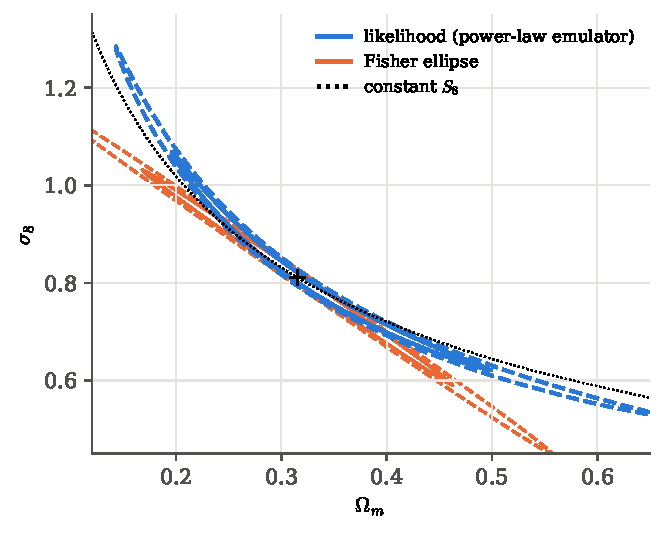
\includegraphics[width=0.62\linewidth]{figures/ch12/w_fisher_cl.pdf}
\caption{The $1\sigma$ and $2\sigma$ regions ($\Delta\chi^2=2.30$, $6.18$) for $(\Omega_m,\sigma_8)$ from the
convergence power spectrum of a KiDS-like $1000\,\mathrm{deg}^2$ survey, $100\le\ell\le3000$, one source bin. The
Fisher ellipse (orange) is the tangent approximation; the likelihood on a grid (blue) curves into a banana along the
dotted line of constant $S_8$.}
\label{12w:fig:fisher-cl}
\end{figure}

\paragraph{How the error depends on the scales used.} With $\ell_{\max}=1500$ instead of $3000$ the forecast becomes
$\sigma(S_8)=\WSigSEightLow$; with $\ell_{\max}=5000$, $\WSigSEightHigh$. The gain flattens because beyond the
crossing multipole, where $C_\ell=N$ ($\ell\approx\WLcrossKiDS$ for our density, $\ell\approx\WLcrossSfour$ for a
Stage-IV density of $30\,\mathrm{arcmin}^{-2}$), each mode carries the factor $[C/(C+N)]^2$ of \cref{T1b:sec:noise-sn}
and adds little.

\subsection{Against the published surveys}
\label{12w:sec:cl-surveys}

\Cref{T1b:sec:s8-surveys} listed the published precisions: $\sigma(S_8)=0.0225$ for KiDS-1000 (symmetrised),
$0.024$ for DES Year~3 and $0.0315$ for HSC Year~1. Our $\WSigSEight$ for a KiDS-like survey is the same size. That
agreement is a coincidence of errors that point in opposite directions, and it is worth taking apart, because each
piece is a choice every analysis makes.
\begin{itemize}[itemsep=1pt,leftmargin=1.2em]
  \item \emph{We use more scales.} KiDS-1000 uses band powers for $100\le\ell\le1500$ \cite{Asgari2021KiDS}, HSC
        $300\le\ell\le1900$ \cite{Hikage2019HSC}; small scales are cut because baryonic feedback and the non-linear
        model are uncertain there (\cref{T1b:sec:objects}). Cutting ours at $1500$ doubles our error, to
        $\WSigSEightLow$.
  \item \emph{We have no nuisance parameters.} Photometric-redshift shifts, the shear calibration $m$, intrinsic
        alignments and baryons are all marginalised in the real analyses. Each adds a direction in parameter space along
        which the spectrum can change, and \eqref{T1b:eq:marg-cost} says what that costs; \cref{12w:sec:research}
        computes the cost of $m$.
  \item \emph{We have no tomography.} KiDS-1000 splits its sources into five redshift bins. Each bin has its own
        exponent $\alpha$ (\cref{T1b:fig:alpha}), so the five needles are not parallel, and their intersection is much
        shorter than any one of them. This is what lets KiDS, with nuisances and a lower $\ell_{\max}$, reach
        $0.0225$ while our single bin to $\ell=1500$ reaches only $\WSigSEightLow$.
  \item \emph{Our covariance is Gaussian.} The non-Gaussian variance, hidden by shape noise in
        \cref{12w:fig:cov-ratio} but present in the signal, and the super-sample term both widen the real errors.
\end{itemize}
The lesson of the comparison: a forecast that matches a published error bar has not been validated by it; only a
forecast that includes the same scales, nuisances and covariance terms can be compared number to number. What we can
do honestly is compare summaries with each other under identical simplifications: whatever the nuisances do to
the spectrum, they do to the peaks and the islands too.
\section{Beyond two points: peaks, shapes and persistence of the mass map}
\label{12w:sec:beyond}

The power spectrum of \cref{12w:sec:twopoint} pins down one combination of $\Omega_m$ and $\sigma_8$ and leaves the
other almost free. \Cref{12w:sec:lognormal} found a property of the map that responds to the two parameters
differently: the lopsidedness of the convergence, whose reduced skewness is $3/\lambda$, set by the empty-beam shift
and so by $\Omega_m$ alone. Two universes on the same $S_8$ line have the same spectrum, but the one with less
matter, more clumped, has rarer and taller peaks and wider, shallower voids. The power spectrum cannot see this; it
is blind to the phases of the Fourier modes, where that arrangement lives (\cref{7b:sec:what-cl-misses}). The peaks,
islands and lakes of the map can.

\paragraph{The question.} For the noisy signal-to-noise map of a KiDS-like survey, how well does each of four
summaries (peak counts, Minkowski functionals, Betti curves, persistent Betti numbers) measure $(\Omega_m,\sigma_8)$,
how much does each add to the power spectrum, and does the gain disappear, as it must, when the map is Gaussian?

\subsection{Four summaries of one map}
\label{12w:sec:summaries}

All four are computed from the same object: the $\kappa_E$ map reconstructed from noisy shear
(\cref{12w:sec:ks-chain}), smoothed with a Gaussian of $\theta_G=3'$ and divided by the rms of the smoothed shape
noise, $\sigma_{\rm noise}=\WSigNoiseSm$ \eqref{12w:eq:sigma-noise}. This is the \newterm{signal-to-noise map}
$\nu(\bm\theta)=\kappa_{E,s}(\bm\theta)/\sigma_{\rm noise}$. The divisor is a fixed number, the same for every
cosmology, so that a threshold $\nu=2$ means the same convergence in every map, and the parameters can move the
summaries. (Dividing each map by its own rms, as one does for a Gaussian field in \cref{12a:sec:excursion}, would
remove the amplitude information we want to keep.) The thresholds are in the range $-1.5\le\nu\le3$, where the
excursion sets are neither empty nor everything.

\begin{itemize}[itemsep=2pt,leftmargin=1.2em]
  \item \emph{Peak counts.} A \newterm{peak} is a pixel higher than all eight of its neighbours. We histogram the
        heights $\nu$ of all peaks in eleven bins from $-1$ to $12$. A peak is a local event; its count at height
        $\nu$ is the number of maxima of the field there, the quantity whose Gaussian average the Kac--Rice method of
        \cref{12a:sec:rice} gives.
  \item \emph{Minkowski functionals.} At each of ten thresholds, the area fraction $V_0$, the boundary length per
        unit area $V_1$ and the Euler characteristic per unit area $V_2$ of the excursion set $\{\nu\ge\nu_t\}$
        (\cref{12a:sec:three}): thirty numbers.
  \item \emph{Betti curves.} At the same thresholds, the number of islands $\beta_0$ and of lakes $\beta_1$ of
        the excursion set (\cref{12b:sec:betti-curve}): twenty numbers. In the plane $V_2\times\text{area}=\beta_0-
        \beta_1$ at every threshold where the set does not wrap around the periodic patch.
  \item \emph{Persistent Betti numbers.} From the persistence diagrams of the superlevel filtration
        (\cref{12b:sec:filtration}), for each pair of thresholds $\nu_{\rm lo}\le\nu_{\rm hi}$ from the grid
        $\{-1,0,1,2,3\}$, the number of islands, and separately of lakes, that exist at every level between them.
\end{itemize}

\begin{workdef}[Persistent Betti number]
Lower a threshold $\nu$ through a map. Each island (or lake) of the excursion set $\{\nu(\bm\theta)\ge\nu\}$ is
born at a level $b$ and dies at a level $d<b$ (\cref{12b:sec:filtration}). The \newterm{persistent Betti number}
\[
\beta_n(\nu_{\rm hi},\nu_{\rm lo})\equiv\#\bigl\{(b,d)\ \text{in the diagram of dimension }n:\ b\ge\nu_{\rm hi}\
\text{and}\ d<\nu_{\rm lo}\bigr\},\qquad\nu_{\rm lo}\le\nu_{\rm hi},
\]
counts the features alive over the whole range $[\nu_{\rm lo},\nu_{\rm hi}]$ \unpack{born at or above the upper
level, not yet dead at the lower one}. For $\nu_{\rm lo}=\nu_{\rm hi}=\nu$ it is the ordinary Betti number
$\beta_n(\nu)$ of \eqref{12b:eq:betti-curve}.
\end{workdef}

This is eq.~(10) of Heydenreich, Br\"uck and Harnois-D\'eraps \cite{Heydenreich2021}, translated. They lower nothing:
they raise a threshold $t$ through the signal-to-noise map and study the sets $\{\nu\le t\}$, the
\newterm{sublevel} filtration, in which a minimum of the map starts a component and a maximum starts a hole. Our
superlevel filtration of $\nu$ is their sublevel filtration of $-\nu$, so their interval $[t_i,t_j)$ is our pair
$(b,d)=(-t_i,-t_j)$ and their condition $t_i\le t\le t'<t_j$ is ours with $\nu_{\rm hi}=-t$, $\nu_{\rm lo}=-t'$. In
our convention the peaks of the map are islands, which matches the way we think of a mass map.

\paragraph{What persistence sees that counts do not: three small maps.}
Heydenreich and collaborators illustrate the difference with three tiny maps \cite[Fig.~4]{Heydenreich2021}, redrawn
in \cref{12w:fig:toy}: a $7\times10$ grid of signal-to-noise values, zero except in a few pixels. Map~1 has four
isolated spikes of heights $4$, $3$, $2$ and $1$. Map~2 has the same four peak heights, but the $4$, the $3$ and the
$2$ sit on one plateau of $1$s and $2$s, with only the $1$ isolated. Map~3 has two separate hills, a $4$ on a ring of
$2$s and a $3$ on a ring of $1$s. Pixels touch through edges and corners, as in \cref{12a:sec:pixels}.

\begin{figure}[htbp]
\centering
\hspace*{4.565cm}\begin{tikzpicture}[x=0.33cm,y=0.33cm]
  \foreach \mapnum/\xoff/\rows in {
      1/0/{{0,0,0,0,0,0,0,0,0,0},{0,0,4,0,0,0,0,0,0,0},{0,0,0,0,0,0,0,1,0,0},{0,0,0,0,0,0,0,0,0,0},{0,0,0,0,0,0,0,0,0,0},{0,2,0,0,0,0,0,0,3,0},{0,0,0,0,0,0,0,0,0,0}},
      2/11/{{0,0,0,0,0,0,0,0,0,0},{0,0,2,2,2,1,1,0,0,0},{0,0,2,4,2,3,1,0,0,0},{0,0,2,2,1,1,1,0,0,0},{0,0,0,0,1,2,1,0,0,0},{0,0,1,0,1,1,1,0,0,0},{0,0,0,0,0,0,0,0,0,0}},
      3/22/{{0,0,0,0,0,0,0,0,0,0},{0,2,2,2,0,0,0,0,0,0},{0,2,4,2,0,0,0,0,0,0},{0,2,2,2,0,0,1,1,1,0},{0,0,0,0,0,0,1,3,1,0},{0,0,0,0,0,0,1,1,1,0},{0,0,0,0,0,0,0,0,0,0}}} {
    \foreach \row [count=\r from 0] in \rows {
      \foreach \v [count=\c from 0] in \row {
        \pgfmathtruncatemacro{\vv}{\v}
        \pgfmathtruncatemacro{\pc}{21*\v}
        \fill[formblue!\pc] (\xoff+\c,-\r) rectangle ++(1,-1);
        \draw[black!25] (\xoff+\c,-\r) rectangle ++(1,-1);
        \ifnum\vv>0 \node[font=\tiny] at (\xoff+\c+0.5,-\r-0.5) {\vv};\fi
      }
    }
    \node[font=\small] at (\xoff+5,0.8) {map \mapnum};
  }
\end{tikzpicture}

\vspace{2mm}
\footnotesize\setlength{\tabcolsep}{0pt}
\begin{tabular}{@{}p{4.4cm}*{3}{>{\centering\arraybackslash}p{3.63cm}}@{}}
\toprule
 & map 1 & map 2 & map 3\\\midrule
peak heights & $4,3,2,1$ & $4,3,2,1$ & $4,3$\\
islands $\beta_0(\nu)$ at $\nu=1,2,3,4$ & $4,3,2,1$ & $2,2,2,1$ & $2,2,2,1$\\
island diagram $(b,d)$ & $(4,\cdot),(3,0),(2,0),(1,0)$ & $(4,\cdot),(3,2),(2,1),(1,0)$ & $(4,\cdot),(3,0)$\\
$\beta_0(\nu_{\rm hi}{=}2,\nu_{\rm lo}{=}1)$ & $3$ & $1$ & $2$\\
\bottomrule
\end{tabular}
\caption{Three signal-to-noise maps after \cite[Fig.~4]{Heydenreich2021} (darker means higher). Peak counts cannot tell
map~1 from map~2; Betti curves cannot tell map~2 from map~3; the persistence diagrams, and the persistent Betti
number in the last row, differ for all three. The dot in $(4,\cdot)$ marks the island that never dies.}
\label{12w:fig:toy}
\end{figure}

Work through them in the order of the question \emph{what does each summary record?}
\emph{Peaks.} A pixel counts if it is higher than all eight neighbours. In map~2 the $3$ (third row) has neighbours
$2,1,1,2,1,1,1,1$, all lower, so it is a peak; so is the $2$ in the fifth row, surrounded by $1$s, and the lone $1$,
surrounded by $0$s. Maps~1 and 2 both have peaks of heights $4,3,2,1$: identical peak counts.
\emph{Betti numbers.} Lower the threshold. In map~2 the set $\{\nu\ge3\}$ is the $4$ and the $3$, two islands
(the $2$ between them is not yet dry); at $\nu=2$ the $2$s join the $4$ and the $3$ into one island while the lower
$2$ appears on its own, still two; at $\nu=1$ the plateau is one island and the lone $1$ another, still two; only
the $4$ is above $4$. So $\beta_0=2,2,2,1$ at $\nu=1,2,3,4$, the same as map~3, where the two hills stay apart at
every level above zero.
\emph{Persistence.} The elder rule of \cref{12b:sec:filtration} records when each island is absorbed. In map~2 the
$3$ is absorbed into the $4$ at level $2$, the pass between them, so its pair is $(3,2)$; the $2$ in the fifth row
joins the plateau at level $1$, $(2,1)$; the lone $1$ joins at $0$, when the background goes dry, $(1,0)$. In maps~1
and 3 every island survives until the background joins it at $0$. The diagrams differ for all three maps. A single
persistent Betti number already separates them: $\beta_0(2,1)$ counts the islands born at or above $2$ that are still
separate at level $1$, which is $3$ in map~1 (the $4$, $3$ and $2$), $1$ in map~2 (only the $4$; the $3$ and the $2$
merged before level $1$) and $2$ in map~3. Peaks record heights, Betti numbers record how many pieces there are at
each level, and persistence records how the pieces are connected across levels: whether a peak stands alone or sits
on the shoulder of a bigger one.

\pyname{w04_beyond.py} repeats the three maps by machine, with the union--find code of \cref{12b:sec:unionfind} and
with its periodic version used for the simulated maps; the diagrams of the two $\WToyOK$ exactly.

The periodic version needs one more idea, for the lakes. On a patch that wraps around, there is no open sea to tell
a lake from the rest of the water, so the trick of \cref{12b:sec:unionfind} (surround the map by sea) is not available.
What is available is a duality between land and water. \emph{When is a lake born?} At the level $s$ where the land
closes a ring around a body of water, which is the level where, seen from the water's side, two water bodies stop
being connected: the pass between them. \emph{When does it die?} At the level $m$ where the last water inside the
ring dries up, which is the water body's lowest point. So a lake of the land with pair $(b,d)=(s,m)$ is the same
object as a water body that, as the level is \emph{raised}, appears at its bottom $m$ and merges with another body at
the pass $s$. Raising the level through $\nu$ is lowering it through $-\nu$, so the water bodies are the islands of
$-\nu$, and the lakes of the map come from the same union--find run on $-\nu$, with four neighbours instead of eight
(two water pixels that touch only at a corner are separated by the land pixels that touch there). The two rings that
wrap around the periodic patch never close up and have no pair; they are left out. The persistence diagrams of all
$\WGudhiN$ fiducial maps were also computed separately, from the same seeds, with \pyname{gudhi}'s
\texttt{PeriodicCubicalComplex} (\pyname{w04b_gudhi_check.py}); the Betti and persistent Betti numbers of the two codes differ by at most
$\WGudhiDev$.

On a simulated $256\times256$ map,
$\beta_0$ from the persistence diagram matches the component count of \pyname{lib_topo} at all ten thresholds (largest
difference $\WDevBzero$), and $\beta_0-\beta_1$ matches the cubical Euler characteristic of \cref{12a:sec:vef} at
every threshold $\nu\ge1$, where nothing wraps around the patch (largest difference $\WDevChi$).

\paragraph{Redundancy between the summaries.} The diagonal of the persistent Betti numbers repeats the Betti curves,
and $V_2$ repeats $\beta_0-\beta_1$. In a combined data vector such exact repetitions make the covariance matrix
singular, and its inverse meaningless. When persistent Betti numbers are combined with Minkowski functionals we
therefore keep only their off-diagonal entries, $\nu_{\rm lo}<\nu_{\rm hi}$, which hold the information the counts at
single levels do not.

\subsection{The machinery: simulated covariance, common random numbers, and a biased Fisher matrix}
\label{12w:sec:mc-fisher}

None of these summaries has a formula for its mean as a function of $(\Omega_m,\sigma_8)$ for a non-Gaussian map,
nor for its covariance. Both come from simulations. The Fisher matrix of a data vector $\bm s$ with mean
$\bm\mu(\params)$ and covariance $\Cmat$ is still $F_{ij}=\partial_i\bm\mu\T\Cmat^{-1}\partial_j\bm\mu$
(eq.~\ref{10a:eq:gauss-fisher}, treating $\bm s$ as Gaussian, which a sum over many peaks or pixels nearly is), but now
every ingredient is estimated, and each estimate has its own error.

\emph{The covariance.} $\WNfidLN$ lognormal maps of the fiducial cosmology, each with independent shape noise, give
the sample covariance $\hat\Cmat$. Its inverse is biased high, and \eqref{8b:eq:hartlap-derived} gives the correction:
multiply $\hat\Cmat^{-1}$ by $(n-p-2)/(n-1)$, with $n$ maps and $p$ entries in the data vector \cite{Hartlap2007}. For
the largest data vector, $p=\WPall$, the factor is $\WHartAll$.

\emph{The derivatives.} At each of $\WNderLN$ seeds we make four maps, with $\Omega_m$ and $\sigma_8$ in turn moved by
$\pm\WDstep\%$, and difference them: $\bm D_k=[\bm s(\theta_i+h_i)-\bm s(\theta_i-h_i)]/2h_i$ for seed $k$, and the
derivative is the average over seeds. Why the same seed for all four? The scatter of a difference is
\begin{equation}
\Var\bigl[s(\theta+h)-s(\theta-h)\bigr]=\Var s(\theta+h)+\Var s(\theta-h)-2\Cov\bigl[s(\theta+h),s(\theta-h)\bigr],
\label{12w:eq:crn}
\end{equation}
and if the two maps share their white noise and their shape noise, they differ only through the small change of
cosmology, the covariance is almost as large as the variances, and the difference is almost noise-free. These are
\newterm{common random numbers}, the antithetic pairs of \cref{6b:sec:antithetic} used the other way round: there
a negative covariance shrinks the variance of a sum, here a positive one shrinks the variance of a difference. For the power spectrum the
cancellation is nearly perfect. For counts it is not: a $10\%$ change of $\sigma_8$ lifts some peaks across a bin
edge and joins some islands, and these whole-unit jumps differ from seed to seed. That is why the steps are
$\pm10\%$ here, twice those of the power spectrum, at the cost of four more CAMB runs (\pyname{w04a_spectra.py}): the
jumps grow in proportion to the step, the difference divided by $2h$ shrinks, and the noise of the derivative falls.

\emph{The bias this noise causes.} Write the estimated derivative as the true one plus an error,
$\hat{\bm d}_i=\bm d_i+\bm\epsilon_i$, with $\langle\bm\epsilon_i\rangle=0$ and, for $N_{\rm der}$ independent seeds,
$\langle\bm\epsilon_i\bm\epsilon_j\T\rangle=\bm\Sigma_{ij}/N_{\rm der}$, where $\bm\Sigma_{ij}$ is the covariance of the
per-seed derivatives $\bm D_k$. The Fisher matrix is quadratic in the derivatives, and a quadratic form of a noisy
vector is biased, exactly as the power of a noisy map is \eqref{8a:eq:cobs-mean}:
\begin{align}
\bigl\langle\hat{\bm d}_i\T\Cmat^{-1}\hat{\bm d}_j\bigr\rangle
&\eqby{1}\bm d_i\T\Cmat^{-1}\bm d_j+\bm d_i\T\Cmat^{-1}\langle\bm\epsilon_j\rangle+\langle\bm\epsilon_i\rangle\T
\Cmat^{-1}\bm d_j+\bigl\langle\bm\epsilon_i\T\Cmat^{-1}\bm\epsilon_j\bigr\rangle
\nonumber\\
&\eqby{2}F_{ij}+\Tr\bigl[\Cmat^{-1}\langle\bm\epsilon_j\bm\epsilon_i\T\rangle\bigr]
\eqby{3}F_{ij}+\frac{\Tr\bigl[\Cmat^{-1}\bm\Sigma_{ji}\bigr]}{N_{\rm der}} .
\label{12w:eq:fisher-bias}
\end{align}
\begin{explain}
  \item Insert $\hat{\bm d}=\bm d+\bm\epsilon$ and multiply out.
  \item The cross terms vanish because $\langle\bm\epsilon\rangle=0$; a number equals its own trace, and
        $\Tr(\bm a\T\mathsf M\bm b)=\Tr(\mathsf M\bm b\bm a\T)$.
  \item The covariance of an average of $N_{\rm der}$ independent terms is that of one term divided by $N_{\rm der}$.
\end{explain}
The bias is positive on the diagonal: noise in the derivatives looks like extra sensitivity. On its own it is small:
for the largest data vector, $\WLAllBias\%$ of the largest diagonal entry. But the quantity we care about is not on
the diagonal. The ellipse is a needle because its two derivative vectors are nearly parallel. With correlation
coefficient $r$ between the two parameter errors, the smallest eigenvalue of $\Fish$, the one that measures the width
across the needle, is a fraction of order $1-r^2$ of the diagonal (for two equal diagonal entries $a$ and off-diagonal
$ra$ the eigenvalues are $a(1\pm r)$, and $1-\abs r\approx(1-r^2)/2$). For the power spectrum $r=\WLClR$, so
$1-r^2\approx0.4\%$ and the smallest eigenvalue is about $0.2\%$ of the diagonal. A bias of $\WLAllBias\%$ of the
diagonal is then larger than the true width: noise in the derivatives turns two parallel vectors into two vectors
at an angle, and an angle is exactly what breaks a degeneracy. The symptom is unmistakable in the Gaussian control
of \cref{12w:sec:beyond-results}: without a correction, the Minkowski functionals of Gaussian maps give a smaller
error on $S_8$ than the power spectrum ($\WGMfSERaw$ against $\WGClSE$), and adding them to the spectrum multiplies
the figure of merit by $\WGClMfGainRaw$. Both are impossible, since for a Gaussian field the spectrum holds all the
information (\cref{7a:sec:grf}).

\begin{pitfall}[A Fisher matrix from simulated derivatives is optimistic]
Estimated derivatives add the positive term \eqref{12w:eq:fisher-bias} to the Fisher matrix, and its effect on the
error along a degeneracy can be larger than the true information. Use common random numbers, steps large enough that
counts change by many units, and many seeds; subtract the bias; and bracket the answer with an estimate that is biased
the other way.
\end{pitfall}

We report three estimates. The \emph{plain} one, $\hat{\bm d}\T\hat\Cmat^{-1}\hat{\bm d}$ with the Hartlap factor, is
biased high. The \emph{corrected} one subtracts \eqref{12w:eq:fisher-bias}, with $\bm\Sigma_{ij}$ estimated from the
scatter of the per-seed derivatives. The \emph{compressed} one splits the seeds in two halves: the first half
defines two combinations of the data vector, $t_i=\hat{\bm d}_i^{(1)\mathsf T}\hat\Cmat^{-1}\bm s$, one per parameter
(a linear compression in the spirit of the score of \cref{10a:sec:two-faces}), and the second half measures how $t$
responds to the parameters; then the halves swap and the two results are averaged. Noisy compression vectors only lose
information, and the second half's noise enters a two-entry vector instead of a $p$-entry one, so this estimate is
biased low. The truth lies between the compressed and the plain values, and the corrected value is our best estimate.

\subsection{What the simulations say}
\label{12w:sec:beyond-results}

The signal-to-noise maps $\nu(\bm\theta)$ of \cref{12w:sec:summaries}, the four summaries computed on them and the
simulated Fisher machinery of \cref{12w:sec:mc-fisher} are all we need. \pyname{w04_beyond.py} makes
$\WNfidLN$ fiducial lognormal maps for the covariance and $\WNderLN$ seeds of four shifted maps each for the
derivatives; then the same again with Gaussian maps of the same spectrum ($\WNfidG$ and $\WNderG$), the control in
which every gain over the power spectrum must vanish. That is $\WNmapsTot$ maps of $256\times256$ pixels. Each patch
is $6.4\times6.4\,\mathrm{deg}$; the Fisher matrices are multiplied by $\WScale$, the number of such patches in a
$1000\,\mathrm{deg}^2$ survey, treating the patches as independent.

\paragraph{How the summaries respond.} \Cref{12w:fig:beyond-response} shows, for four of the summaries, how the
mean of each entry moves when $\ln\sigma_8$ or $\ln\Omega_m$ changes, in units of the scatter of that entry on one
patch. More clumping (larger $\sigma_8$) moves peaks from the middle heights to the top: fewer peaks at $\nu\approx1$,
more above $\nu\approx3$. The Euler characteristic and the island count follow the same pattern, since at high
thresholds islands are almost all there is, and the lakes respond where the excursion set is mostly land, below
$\nu\approx0$. The two curves in each panel have nearly the same shape, the $\Omega_m$ curve about half the
$\sigma_8$ curve.

\begin{figure}[htbp]
\centering
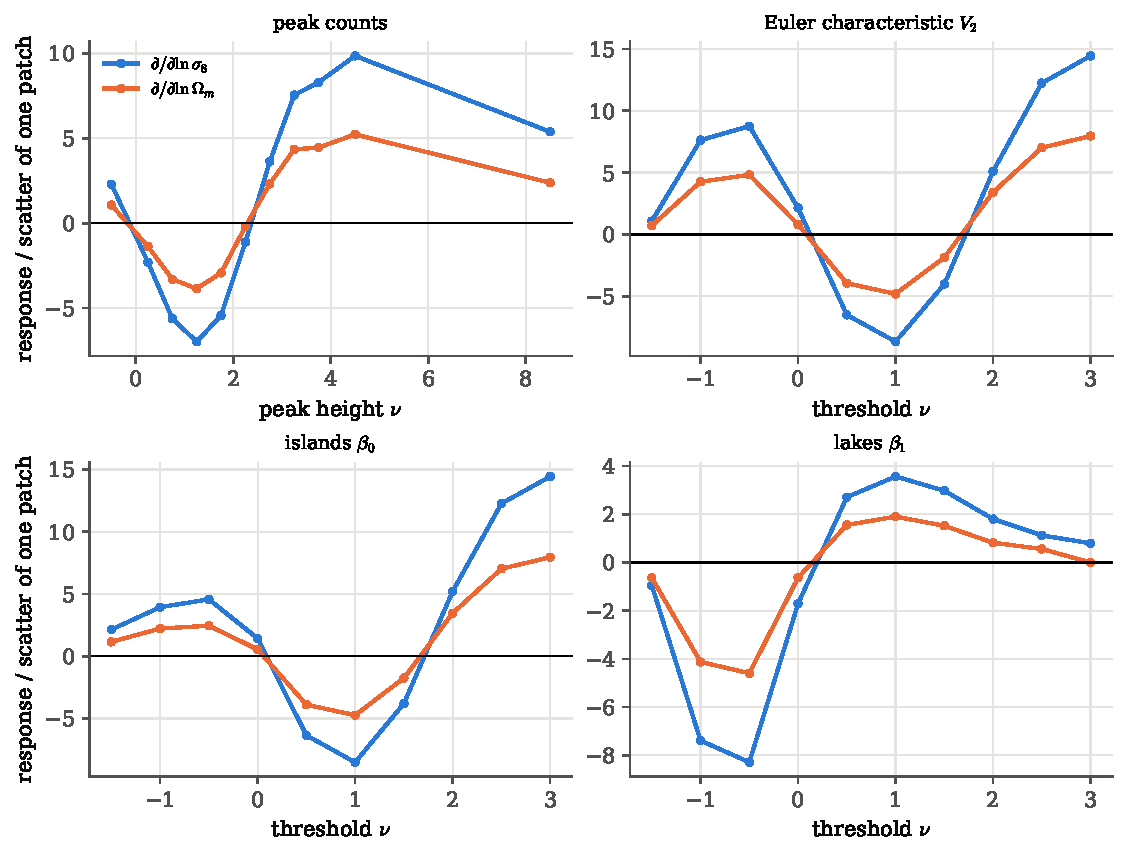
\includegraphics[width=0.92\linewidth]{figures/ch12/w_beyond_response.pdf}
\caption{The response of four summaries of the signal-to-noise map to $\ln\sigma_8$ (blue) and $\ln\Omega_m$ (orange),
each divided by the scatter of that entry on one $41\,\mathrm{deg}^2$ patch. The orange curve is nearly the blue one
halved: this is the $S_8$ degeneracy, entry by entry. The small departures from exact proportionality are what lets a
summary measure the two parameters separately.}
\label{12w:fig:beyond-response}
\end{figure}

\paragraph{Example: reading the degeneracy off the responses.}
Suppose every entry $\mu_a$ of a summary had $\partial\mu_a/\partial\ln\Omega_m=\alpha\,\partial\mu_a/
\partial\ln\sigma_8$ with one number $\alpha$ for all $a$. Move the parameters by $\delta\ln\sigma_8$ and
$\delta\ln\Omega_m$:
\begin{align}
\delta\mu_a
&\eqby{1}\frac{\partial\mu_a}{\partial\ln\sigma_8}\,\delta\ln\sigma_8+\frac{\partial\mu_a}{\partial\ln\Omega_m}\,
\delta\ln\Omega_m
\eqby{2}\frac{\partial\mu_a}{\partial\ln\sigma_8}\bigl(\delta\ln\sigma_8+\alpha\,\delta\ln\Omega_m\bigr)
\eqby{3}\frac{\partial\mu_a}{\partial\ln\sigma_8}\;\delta\ln\bigl(\sigma_8\Omega_m^{\alpha}\bigr).
\label{12w:eq:resp-degen}
\end{align}
\begin{explain}
  \item First-order Taylor expansion of the mean in the two log-parameters.
  \item The assumed proportionality of the two responses.
  \item $\delta\ln\sigma_8+\alpha\,\delta\ln\Omega_m=\delta\ln(\sigma_8\Omega_m^\alpha)$.
\end{explain}
Every entry would then move only through the single combination $\sigma_8\Omega_m^\alpha$; a change along the line
$\sigma_8\Omega_m^\alpha=$ const would change nothing, and the Fisher matrix would have a zero eigenvalue. With
the ratio of about one half read from \cref{12w:fig:beyond-response}, the combination is close to
$\sigma_8\Omega_m^{0.5}\propto S_8$: the peaks, islands and lakes of the map feel the same degeneracy as the power
spectrum, for the same reason (the amplitude of the convergence is set mainly by $S_8$, \cref{T1b:sec:s8}).
Whatever a summary measures beyond $S_8$ comes from the entries where the ratio differs from one half, which is why
the derivative noise of \eqref{12w:eq:fisher-bias}, which also changes that ratio, is so dangerous.

\paragraph{The numbers.} \Cref{12w:tab:beyond} lists, for each summary and for its combination with the power
spectrum, the forecast error on $S_8$ and the figure of merit $1/\sqrt{\det\bm\Sigma}$ of \cref{10a:sec:fom}, where
$\bm\Sigma=\Fish^{-1}$ is the $2\times2$ covariance of $(\Omega_m,\sigma_8)$, divided by that of the power spectrum
alone. All use the corrected estimate of \cref{12w:sec:mc-fisher}; the plain estimate of the Gaussian control is
shown too, to make the bias visible.

\begin{table}[htbp]
\centering
\small
\begin{tabular}{@{}lccccc@{}}
\toprule
 & \multicolumn{2}{c}{lognormal maps} & \multicolumn{3}{c}{Gaussian maps (control)}\\
\cmidrule(lr){2-3}\cmidrule(l){4-6}
summary & $\sigma(S_8)$ & FoM$/$FoM$_{C_\ell}$ & $\sigma(S_8)$ & FoM$/$FoM$_{C_\ell}$ & plain estimate\\\midrule
$C_\ell$ ($\WLClP$ bands) & $\WLClSE$ & $1$ & $\WGClSE$ & $1$ & $1$\\
peaks ($\WLPkP$) & $\WLPkSE$ & $\WLPkGain$ & -- & -- & $\WGPkGainRaw$\\
Minkowski ($\WLMfP$) & $\WLMfSE$ & $\WLMfGain$ & $\WGMfSE$ & $\WGMfGain$ & $\WGMfGainRaw$\\
Betti ($\WLBettiP$) & $\WLBettiSE$ & $\WLBettiGain$ & $\WGBettiSE$ & $\WGBettiGain$ & $\WGBettiGainRaw$\\
persistent Betti ($\WLPbettiP$) & $\WLPbettiSE$ & $\WLPbettiGain$ & $\WGPbettiSE$ & $\WGPbettiGain$ & $\WGPbettiGainRaw$\\\midrule
$C_\ell$ + peaks & $\WLClPkSE$ & $\WLClPkGain$ & $\WGClPkSE$ & $\WGClPkGain$ & $\WGClPkGainRaw$\\
$C_\ell$ + Minkowski & $\WLClMfSE$ & $\WLClMfGain$ & $\WGClMfSE$ & $\WGClMfGain$ & $\WGClMfGainRaw$\\
$C_\ell$ + Betti & $\WLClBettiSE$ & $\WLClBettiGain$ & $\WGClBettiSE$ & $\WGClBettiGain$ & $\WGClBettiGainRaw$\\
$C_\ell$ + persistent Betti & $\WLClPbettiSE$ & $\WLClPbettiGain$ & $\WGClPbettiSE$ & $\WGClPbettiGain$ &
$\WGClPbettiGainRaw$\\
all four & $\WLAllSE$ & $\WLAllGain$ & $\WGAllSE$ & $\WGAllGain$ & $\WGAllGainRaw$\\
\bottomrule
\end{tabular}
\caption{Forecasts for $(\Omega_m,\sigma_8)$ from a KiDS-like $1000\,\mathrm{deg}^2$ survey, one source bin, from each
summary of the signal-to-noise map and from its combination with the power spectrum. The number of entries of each data
vector (lognormal case) is in brackets; entries that never change are dropped. FoM is the figure of merit $1/\sqrt{\det\bm\Sigma}$; for the power
spectrum it is $\WLClFom$ (lognormal) and $\WGClFom$ (Gaussian). The last column is the FoM ratio of the Gaussian
control before the derivative-noise bias is subtracted. For Gaussian maps the corrected peak matrix is not
positive: its measured width across the needle is pure noise.}
\label{12w:tab:beyond}
\end{table}

\emph{The control first.} For Gaussian maps, adding any summary to the power spectrum must leave the figure of merit
unchanged, because the spectrum holds all the information about a Gaussian field. The corrected estimates give
gains between $\WGClPkGain$ and $\WGClPbettiGain$, above one by up to about ten per cent: that excess is the
residual error of our estimator, and any lognormal gain smaller than it means nothing. The plain estimates give gains
up to $\WGClMfGainRaw$, and would have announced a discovery. On their own, the counts of a Gaussian map are much
weaker than its spectrum (FoM ratios between $\WGPbettiGain$ and $\WGBettiGain$, and for the peaks so little that
the corrected matrix is not even positive): they see the amplitude through the heights in units of a fixed
$\sigma_{\rm noise}$, but they lose the scale information of eight separate bands.

\emph{Now the lognormal maps.} Each summary alone is roughly as strong as the power spectrum: the Minkowski
functionals match its figure of merit ($\WLMfGain$), and peaks fall a little short of it ($\WLPkGain$) but give a
smaller error on $S_8$ ($\WLPkSE$ against $\WLClSE$, $\WLPkOverClSE\%$ less). The Betti curves and the persistent Betti
numbers are weaker, about half the figure of merit of the spectrum. Combined with the spectrum, every summary helps
by far more than the ten per cent the control allows: peaks multiply the figure of merit by $\WLClPkGain$, Minkowski
functionals by $\WLClMfGain$, Betti and persistent Betti numbers by about $\WLClBettiGain$, and all four together by
$\WLAllGain$, with $\sigma(S_8)$ down by $\WLAllSEgain\%$. \Cref{12w:fig:beyond-fisher} shows why the combination does
so much more than the parts. All the ellipses are needles along the same $S_8$ line; they differ slightly in angle,
and two needles at a slight angle cross in a short segment.

\begin{figure}[htbp]
\centering
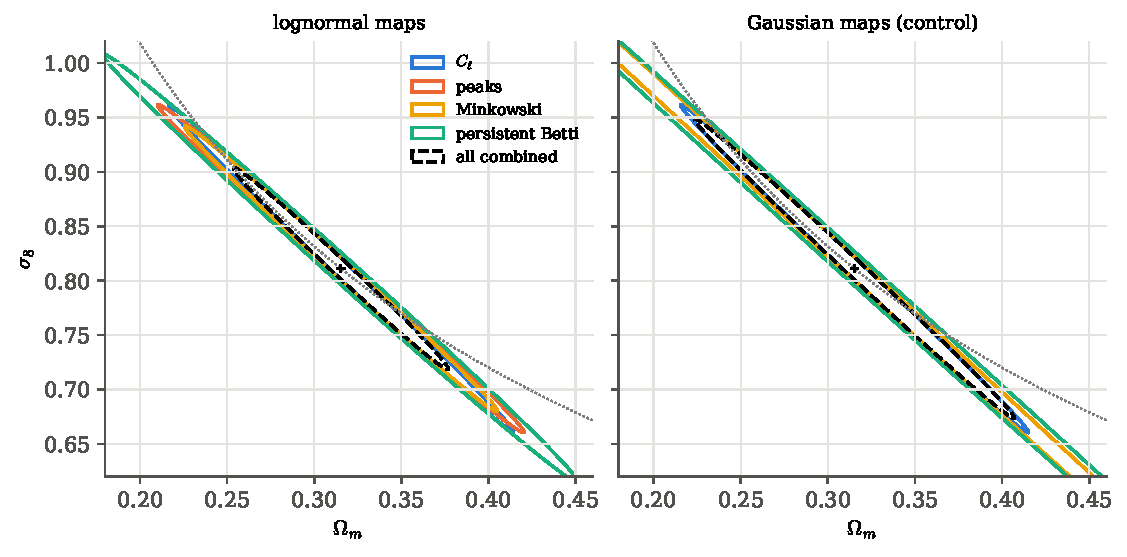
\includegraphics[width=0.95\linewidth]{figures/ch12/w_beyond_fisher.pdf}
\caption{The $1\sigma$ Fisher ellipses ($\Delta\chi^2=2.30$) of $(\Omega_m,\sigma_8)$ for a $1000\,\mathrm{deg}^2$
survey, with the derivative-noise bias subtracted. Left: lognormal maps; the dashed ellipse, all four summaries
together, is the shortest. Right: Gaussian maps of the same spectrum; the combination is hardly shorter than the power
spectrum, as it must be. The dotted curve is the line of constant $S_8$. The Gaussian peak ellipse is missing
because its corrected Fisher matrix is not positive.}
\label{12w:fig:beyond-fisher}
\end{figure}

\emph{Where the extra information comes from.} \Cref{12w:sec:lognormal} gave the answer before any simulation: the
reduced skewness of a lognormal map is $3/\lambda$, and the empty-beam depth $\lambda$ depends on $\Omega_m$ but not on
$\sigma_8$. Two universes on the same $S_8$ line have the same spectrum but differently lopsided maps. Every one of our
summaries sees the lopsidedness: the peak heights through the long upper tail, the Minkowski functionals and Betti
numbers through the asymmetry between high and low thresholds. That is the lever on the valley, and the Gaussian
control, which has no lopsidedness, has no lever.

\paragraph{Example: how much a covariance from simulations costs.}
The Hartlap factor $(n-p-2)/(n-1)$ of \eqref{8b:eq:hartlap-derived} rescales the inverse covariance. For all four
summaries together, $p=\WPall$ entries from $n=\WNfidLN$ maps:
\begin{align*}
\frac{n-p-2}{n-1}=\frac{1000-65-2}{999}\eqby{1}0.934,\qquad
\frac{\sigma_{\rm corrected}}{\sigma_{\rm naive}}\eqby{2}\Bigl(\frac{n-p-2}{n-1}\Bigr)^{-1/2}=1.03 .
\end{align*}
\begin{explain}
  \item Arithmetic: $933/999$.
  \item The Fisher matrix is proportional to $\hat\Cmat^{-1}$, so it shrinks by the factor, and errors, which go as
        $\Fish^{-1/2}$, grow by its inverse square root.
\end{explain}
A $3\%$ correction. With the $126$ simulations that Heydenreich and collaborators used for their covariance
\cite{Heydenreich2021}, the same data vector would have $(126-65-2)/125=0.47$: errors $46\%$ larger, and the
correction itself uncertain. That is why they kept their data vectors short and why they used the $t$-likelihood of
\cref{12w:sec:research} instead of the factor. Simulations for the covariance are the hidden price of every summary
with many entries.

\paragraph{Example: what a figure-of-merit ratio means for the ellipse.}
For a $2\times2$ covariance $\bm\Sigma$ the ellipse $\Delta\chi^2=q$ has area $\pi q\sqrt{\det\bm\Sigma}$
(\cref{10a:sec:fom}), so the ratio of two figures of merit is the inverse ratio of the areas of their ellipses, at any
confidence level. All four summaries together with the spectrum have $\WLAllGain$ times the figure of merit of the
spectrum alone, so their ellipse covers the fraction $1/\WLAllGain$ of the area. Which dimension shrank? The area of a
needle is its length times its width. The width, the error on the best-measured combination $\sigma_8\Omega_m^\alpha$,
is set by the overall amplitude of the map, which the spectrum already measures well. The length is the error along
the valley, which shows up as the error on $\Omega_m$; it falls from $\WLClOm$ to $\WLAllOm$. Almost all of the gain
is a shorter needle. The error on $S_8$ falls by about the same fraction, from $\WLClSE$ to $\WLAllSE$, because, as
\eqref{12w:eq:s8-tilt} showed, $\sigma(S_8)$ is mostly the small tilt between the needle and the line of constant
$S_8$ times the needle's length.

\paragraph{Which peaks carry the information?} Splitting the peak histogram into low ($\nu<0.5$), medium
($0.5\le\nu<2.5$) and high ($\nu\ge2.5$) peaks and computing the Fisher matrix of each part alone gives figures of
merit $\WPkLowFom$, $\WPkMidFom$ and $\WPkHighFom$ (errors on $S_8$ of $\WPkLowSE$, $\WPkMidSE$ and $\WPkHighSE$).
The low peaks, which in a noisy map are mostly noise bumps in underdense regions, carry little. The rest is shared
between the medium and the high peaks; in units of the convergence the high group starts at
$2.5\sigma_{\rm noise}\approx0.026$, well below the height of the peaks made by single massive clusters. The two papers that first asked the question looked at the same split, and their answer
is compared with ours below.

\begin{keyidea}
A summary beyond the power spectrum adds information only to the extent that the field is non-Gaussian. Measure the
gain against a Gaussian control with the same spectrum, with the bias of simulated derivatives removed. For lognormal
convergence maps of a KiDS-like survey every summary adds to the spectrum, all of them together multiplying the
figure of merit by about $\WLAllGain$; for Gaussian maps the gain is zero within the ten-per-cent error of the method.
\end{keyidea}

\subsection{Three published results, reproduced}
\label{12w:sec:beyond-repro}

Three papers asked, in turn, whether peaks are worth counting, whether they add to the two-point analysis, and
whether persistence adds to the peaks. Each compared summaries by the area of a confidence region, so the one
quantity to settle first is that area.

\paragraph{The yardstick.} Dietrich and Hartlap define the figure of merit as one over the area of the $95\%$
region in the $(\Omega_m,\sigma_8)$ plane \cite{DietrichHartlap2010}; Heydenreich and collaborators as one over the
area of the $1\sigma$ region \cite{Heydenreich2021}; we use $1/\sqrt{\det\bm\Sigma}$. \emph{How are they related?}
For a Gaussian posterior the region is the ellipse $\Delta\chi^2\le q$, of area $\pi q\sqrt{\det\bm\Sigma}$
(\cref{10a:sec:fom}), and $q$ is fixed by the probability it must hold. With two parameters $\Delta\chi^2$ follows the
$\chi^2$ distribution with two degrees of freedom, whose density is $\tfrac12e^{-x/2}$ (\cref{ch:02}), so
\begin{align}
\Prob(\Delta\chi^2>q)&\eqby{1}\int_q^\infty\tfrac12e^{-x/2}\,\dd x\eqby{2}e^{-q/2},
\nonumber\\
q_{95\%}&\eqby{3}-2\ln0.05=5.99,\qquad q_{1\sigma}\eqby{4}-2\ln0.317=2.30,
\label{12w:eq:fom-q}
\end{align}
\begin{explain}
  \item The probability outside the ellipse is the tail of the $\chi^2_2$ density.
  \item The antiderivative of $\tfrac12e^{-x/2}$ is $-e^{-x/2}$.
  \item Set the tail to $5\%$ and solve for $q$.
  \item ``$1\sigma$'' in two dimensions means the same $68.3\%$ as in one, so the tail is $31.7\%$.
\end{explain}
and the three figures of merit are $1/(\pi\times5.99\sqrt{\det\bm\Sigma})$, $1/(\pi\times2.30\sqrt{\det\bm\Sigma})$
and $1/\sqrt{\det\bm\Sigma}$. They differ by constant factors, so \emph{the ratio} of the figures of merit of two
summaries is the same in all three conventions, $\sqrt{\det\bm\Sigma_B/\det\bm\Sigma_A}$. That ratio is what we
compare. The absolute values also depend on the survey area $A$: every Fisher matrix grows in proportion to $A$, so
$\bm\Sigma\propto1/A$, $\det\bm\Sigma\propto1/A^2$, and the figure of merit grows in proportion to $A$.

\subsubsection{Peaks, and what shape noise does to them}
\label{12w:sec:repro-kratochvil}

\paragraph{Their question.} In 2009, cluster counts were a strong probe of dark energy, but finding clusters and
weighing them brings selection effects. Kratochvil, Haiman and May asked whether one could skip the clusters and
count the peaks of the lensing map itself, as a function of height, and still tell cosmological models apart
\cite{Kratochvil2010}.

\paragraph{Their setup.} $N$-body simulations of three models with dark-energy equation of state $w=-0.8$, $-1$ and
$-1.2$, with the same primordial amplitude, so that $\sigma_8$ differs ($0.742$, $0.798$, $0.839$). Convergence maps
of $3\times3\,\mathrm{deg}$ by ray tracing, for sources at $z_s=2$; shape noise of $15$ galaxies per arcmin$^2$
added pixel by pixel; Gaussian smoothing with $\theta_G=1'$ in their convention (a standard deviation of $0.71'$,
\cref{12w:sec:ks-noise}); a peak is a pixel higher than its eight neighbours, as for us; peaks histogrammed in bins of
$\kappa$; covariance from $200$ pseudo-independent maps.

\paragraph{Their key equation.} How well can a histogram of peak counts $\bm N$ separate two models? They use
$\chi^2=\Delta\bm N\T\Cmat^{-1}\Delta\bm N$ with $\Delta\bm N$ the difference of the mean histograms
\cite[eq.~14]{Kratochvil2010}. For two nearby models, separated by $\Delta\params$, this is our Fisher matrix:
\begin{equation}
\Delta\bm N\T\Cmat^{-1}\Delta\bm N\eqby{1}\Bigl(\sum_i\frac{\partial\bm N}{\partial\theta_i}\Delta\theta_i\Bigr)\T
\Cmat^{-1}\Bigl(\sum_j\frac{\partial\bm N}{\partial\theta_j}\Delta\theta_j\Bigr)
\eqby{2}\sum_{ij}\Delta\theta_i\,F_{ij}\,\Delta\theta_j .
\label{12w:eq:krat-chi2}
\end{equation}
\begin{explain}
  \item First-order Taylor expansion of the mean histogram.
  \item Collect the terms; $F_{ij}=\partial_i\bm N\T\Cmat^{-1}\partial_j\bm N$ is \eqref{10a:eq:gauss-fisher}.
\end{explain}
So ``which peaks distinguish the models best'' is ``which peaks contribute most to $\Fish$'', the question of which peaks carry the
information, asked at the end of \cref{12w:sec:beyond-results}. Their noise level is the $\sigma_{\rm noise}=0.0227$ worked out in the
example of \cref{12w:sec:ks-noise}, from \eqref{12w:eq:sigma-noise}.

\paragraph{What they found, and what we compute.} Shape noise raised the total number of peaks in a noise-free
smoothed map from $1646$ to $2432$, by about $50\%$, and the peaks of medium height, $0\lesssim\kappa\lesssim0.06$, most
of them not caused by any single cluster, carried most of the power to separate the models; the low peaks,
$\kappa\lesssim0$, carried little. \pyname{w04_beyond.py} counts the peaks of $50$ lognormal maps with and without
shape noise (\cref{12w:fig:beyond-peaks}) and, from the full Fisher run, the information in low, medium and high peaks.

\begin{figure}[htbp]
\centering
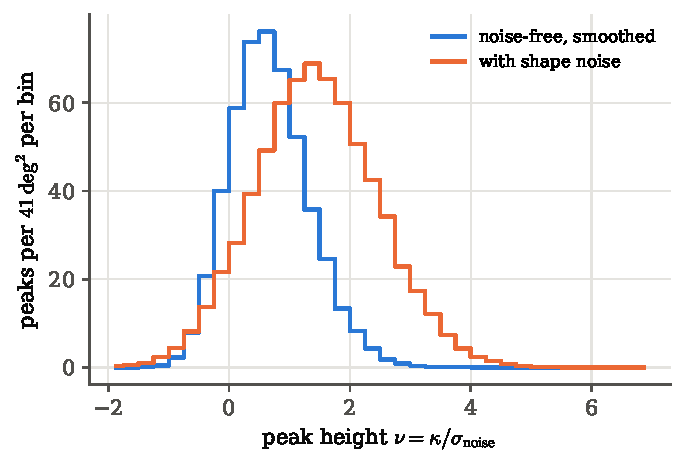
\includegraphics[width=0.62\linewidth]{figures/ch12/w_beyond_peaks.pdf}
\caption{Mean histograms of peak heights on one $41\,\mathrm{deg}^2$ lognormal patch, smoothed with $\theta_G=3'$,
without (blue) and with (orange) shape noise, heights in units of the smoothed noise rms. Noise adds peaks and pushes
the existing ones up and down, so the histogram widens and shifts to larger $\nu$.}
\label{12w:fig:beyond-peaks}
\end{figure}

\paragraph{Side by side.}
\begin{center}
\small
\begin{tabular}{@{}lcc@{}}
\toprule
 & Kratochvil et al.\ (2010) & here\\\midrule
peaks per map, noise-free $\to$ noisy & $1646\to2432$ ($+48\%$) & $\WNpkClean\to\WNpkNoisy$ ($+\WPkBoost\%$)\\
smoothed noise rms $\sigma_{\rm noise}$ & $0.0227$ & $\WSigNoiseSm$\\
least informative peaks & low, $\kappa\lesssim0$ & low, $\nu<0.5$ (FoM $\WPkLowFom$)\\
most informative peaks & medium, $0\lesssim\kappa\lesssim0.06$ & $\nu\ge0.5$ (FoM $\WPkMidFom$, $\WPkHighFom$)\\
\bottomrule
\end{tabular}
\end{center}

\paragraph{Why they differ.} The boost agrees in kind, $+48\%$ against $+\WPkBoost\%$, and the difference of a few points is not
something our single lognormal family can isolate: the smoothing is about four times wider in standard deviation
than theirs, which changes the number of noise maxima per square degree (the Kac--Rice count of \cref{12a:sec:rice},
a few $\theta_G^2$ per maximum) and the share of the smoothed map that is noise, and the maps differ in the strength
of their non-Gaussian peaks. Our split by height is in units of $\sigma_{\rm noise}$ rather than of $\kappa$; translated, our
high bin starts at $\kappa\approx0.026$, inside their medium range, and their result and ours agree that the
information sits a few noise levels up, among peaks made by several structures along the line of sight, and not in
the rare tall peaks of single clusters. Their maps are $N$-body maps of three dark-energy models, ours lognormal maps
varied in $(\Omega_m,\sigma_8)$, so only these qualitative statements carry over.

\paragraph{The lesson.} Shape noise does not just blur the peaks of the mass map, it makes new ones, and they sit on
the signal; a peak count is only meaningful when the simulations it is compared with carry the same noise, processed
the same way.

\subsubsection{Peaks against, and with, cosmic shear}
\label{12w:sec:repro-dh}

\paragraph{Their question.} If most peaks are not clusters, are they just a noisy rewrite of the two-point function,
or do they hold something else? Dietrich and Hartlap measured how well shear peaks constrain $(\Omega_m,\sigma_8)$
compared with cosmic shear, and how much the two do together \cite{DietrichHartlap2010}.

\paragraph{Their setup.} $158$ $N$-body simulations spread over the $(\Omega_m,\sigma_8)$ plane and $35$ more at the
fiducial cosmology, ray-traced into $175$ independent $6\times6\,\mathrm{deg}$ fields; a CFHTLS-like survey of
$180\,\mathrm{deg}^2$ with $25$ galaxies per arcmin$^2$ and total ellipticity dispersion $\sigma_\varepsilon=0.38$
(that is $0.27$ per component, the same as ours); peaks of the aperture-mass signal-to-noise map, a smoothed
convergence map with a compensated filter; a Gaussian likelihood whose inverse covariance from the $175$ fiducial
fields carries the Hartlap factor \cite[eq.~12]{DietrichHartlap2010}, our \eqref{8b:eq:hartlap-derived}.

\paragraph{Their key equation} is the figure of merit, one over the area of the $95\%$ region, which by
\eqref{12w:eq:fom-q} is $1/(\pi\times5.99\sqrt{\det\bm\Sigma})$ for a Gaussian posterior. For a survey of
$180\,\mathrm{deg}^2$ instead of our $1000$, our figures of merit are multiplied by $180/1000$.

\paragraph{Side by side.} Our power spectrum, peaks and their combination, in their convention and for their area:
\begin{center}
\small
\begin{tabular}{@{}lcccc@{}}
\toprule
 & \multicolumn{2}{c}{Dietrich \& Hartlap (2010)} & \multicolumn{2}{c}{here}\\
\cmidrule(lr){2-3}\cmidrule(l){4-5}
 & FoM & ratio to shear & FoM & ratio to $C_\ell$\\\midrule
cosmic shear ($C_\ell$ here) & $71$ & $1$ & $\WLClFomDH$ & $1$\\
peaks & $123$ & $1.73$ & $\WLPkFomDH$ & $\WLPkOverCl$\\
combined & $173$ & $2.44$ & $\WLClPkFomDH$ & $\WLClPkOverCl$\\
\bottomrule
\end{tabular}
\end{center}
The combined value is $1.41$ times their peaks alone\footnote{Their text says the combination has a figure of merit
about $40\%$ larger than cosmic shear alone; their Table~2 makes it $40\%$ larger than the peaks alone and $2.4$ times
cosmic shear alone.}; ours is $\WLClPkOverPk$ times our peaks alone.

\paragraph{Why they differ.} \emph{The absolute values}: their galaxy density is four times ours, so the noise power
$\sigma_e^2/\bar n$ is four times smaller and more multipoles are signal-dominated (\cref{12w:sec:cl-fisher}); their
$N$-body maps carry the non-linear structure our lognormal maps lack; and their regions are the real, curved
likelihood contours, cut by a flat prior, while ours are Fisher ellipses. \emph{The ratios}: their peak statistic
used almost exact source redshifts, while their cosmic shear used only two redshift bins, a mismatch they point out
themselves; ours uses one source bin for both, and the peaks lose the scale-by-scale information of the spectrum.
What survives is the shape of the result: peaks alone are comparable to the two-point analysis, and the combination
beats both by a large factor, larger than either alone.

\paragraph{The lesson.} Two summaries with the same degeneracy are not redundant: their needles differ by a small
angle, and that angle, not the length of either needle, decides the gain of the combination.

\subsubsection{Persistence against peaks}
\label{12w:sec:repro-heydenreich}

\paragraph{Their question.} A peak count records the height of each maximum and nothing about its surroundings.
Heydenreich, Br\"uck and Harnois-D\'eraps asked whether the persistent Betti numbers of the signal-to-noise map, which
also record how features are connected across levels (the three small maps of \cref{12w:fig:toy}), constrain
cosmology better than peaks \cite{Heydenreich2021}.

\paragraph{Their setup.} Aperture-mass signal-to-noise maps of mock KiDS+VIKING-450 data (and, in a second test, of a
$100\,\mathrm{deg}^2$ Euclid-like survey with $30$ galaxies per arcmin$^2$); their means emulated by a Gaussian process
trained on the $26$ cosmologies of the cosmo-SLICS; the covariance from $126$ SLICS runs, with the $t$-likelihood of
Sellentin and Heavens; four parameters ($\Omega_m$, $S_8$, $h$, $w_0$) sampled by MCMC; persistent Betti numbers
evaluated at the pairs of levels that best separate cosmologies, chosen on a dense grid.

\paragraph{Their key equation} is the persistent Betti number of the working definition in \cref{12w:sec:summaries},
their eq.~(10) translated into our superlevel convention, and the figure of merit, one over the area of the $1\sigma$
region, which by \eqref{12w:eq:fom-q} has the same ratios as ours.

\paragraph{Side by side.}
\begin{center}
\small
\begin{tabular}{@{}lcc@{}}
\toprule
 & Heydenreich et al.\ (2021) & here (lognormal)\\\midrule
FoM, persistent Betti $/$ peaks & $1.44$ (KV450-like) & $\WLPbOverPk$\\
$\sigma(S_8)$, persistent Betti vs peaks & $0.045$ vs $0.048$ (KV450) & $\WLPbettiSE$ vs $\WLPkSE$\\
 & $0.027$ vs $0.033$ (Euclid) & \\
$\sigma(S_8)$, persistent Betti vs Betti & $0.045$ vs $0.048$ (KV450) & $\WLPbettiSE$ vs $\WLBettiSE$\\
\bottomrule
\end{tabular}
\end{center}
We do not reproduce their result. In our maps the persistent Betti numbers are no better than the Betti curves and
weaker than the peaks.

\paragraph{Why they differ.} The main reason can be derived. Our map before noise is $\kappa=\lambda[e^{G-s^2/2}-1]$
\eqref{12w:eq:lognormal}, an increasing function of a Gaussian field $G$. For any level $k>-\lambda$,
\begin{equation}
\{\bm\theta:\ \kappa(\bm\theta)\ge k\}
\eqby{1}\Bigl\{\bm\theta:\ e^{G(\bm\theta)-s^2/2}\ge1+\frac k\lambda\Bigr\}
\eqby{2}\Bigl\{\bm\theta:\ G(\bm\theta)\ge\frac{s^2}2+\ln\Bigl(1+\frac k\lambda\Bigr)\Bigr\}.
\label{12w:eq:ln-monotone}
\end{equation}
\begin{explain}
  \item Divide by $\lambda>0$ and add $1$.
  \item The logarithm is increasing, so it keeps the inequality.
\end{explain}
Every superlevel set of the lognormal map \emph{is} a superlevel set of the Gaussian map, at a relabelled level. So
every island and lake, every merger and the pass where it happens, is the Gaussian field's; only the heights at which
they happen are moved. The persistence diagram of a noise-free lognormal map is the Gaussian diagram with its axes
stretched, and the stretch depends on the cosmology only through $\lambda$ and $s$, the one-point distribution that
peak heights already see. Smoothing and noise, applied after the exponential, blur this exact correspondence, but they
do not create the thing persistence was designed to see. Heydenreich and collaborators trace their gain to exactly that
thing: whether peaks stand alone or sit together on a larger overdensity, the environment of haloes in filaments and
superclusters \cite[§4]{Heydenreich2021}, which $N$-body maps have and lognormal maps do not. Their gain also grew
with the galaxy density, as it should if it comes from resolving that structure. Smaller differences push the same
way: their levels were chosen for their power to separate cosmologies, ours form a fixed grid of five, whose diagonal
repeats the Betti curves; and their persistent Betti errors include the error of their emulator, without which their gain on $S_8$ in the
KV450-like case rises from $5\%$ to $8\%$.

\paragraph{The lesson.} A gain from topology is a property of the maps, not of the method. Lognormal maps are a fair
test of the machinery (the covariance, the derivatives, the Fisher bias) and an unfair test of persistence, because
they contain no structure for persistence to find that the one-point distribution does not already give.

\paragraph{The three reproductions together.}
\begin{center}
\small
\begin{tabular}{@{}p{4.3cm}ccp{4.2cm}@{}}
\toprule
result & theirs & ours & main reason for the difference\\\midrule
noise boost of peak counts & $+48\%$ & $+\WPkBoost\%$ & wider smoothing\\
FoM, peaks $/$ two-point & $1.73$ & $\WLPkOverCl$ & their peaks had redshifts, their shear two bins\\
FoM, combined $/$ two-point & $2.44$ & $\WLClPkOverCl$ & as above; density, $N$-body\\
FoM, persistent Betti $/$ peaks & $1.44$ & $\WLPbOverPk$ & lognormal maps have no environment\\
\bottomrule
\end{tabular}
\end{center}
Each published gain beyond the power spectrum appears in our maps exactly as far as the maps contain the structure
behind it: the skewness of a lognormal field, yes; the clustering of haloes, no.
\section{How it is done in research, and what our simplifications cost}
\label{12w:sec:research}

Every number computed so far came from a chain that a real survey also runs, link for link, but with each link
simplified until it fits in a few minutes on a laptop. The chain of \cref{T1b:fig:pipeline} runs from the matter
field to the summaries, with nuisances entering at every step. \Cref{12w:fig:research} sets our version beside the
research version. For each link the surveys do something heavier, we did something cheaper, and the difference has a
price in the width of the error bars.

\begin{figure}[htbp]
\centering
\begin{tikzpicture}[
  box/.style={draw=accent,rounded corners=2pt,fill=ideabg,align=center,font=\scriptsize,
              minimum width=2.45cm,minimum height=1.0cm,inner sep=2pt,text width=2.4cm},
  ours/.style={draw=tangentgreen,rounded corners=2pt,fill=takebg,align=center,font=\scriptsize,
              minimum width=2.45cm,minimum height=1.0cm,inner sep=2pt,text width=2.4cm},
  arr/.style={->,thick,accent}]
  \node[font=\small\bfseries,anchor=east] at (-1.5,0) {research};
  \node[font=\small\bfseries,anchor=east] at (-1.5,-1.8) {here};
  \node[box] (r1) at (0,0)    {$N$-body + ray tracing,\\ $10^2$--$10^3$ runs};
  \node[box] (r2) at (2.85,0) {catalogue: PSF, shear\\ calibration, photo-$z$};
  \node[box] (r3) at (5.7,0)  {masked sphere,\\ tomography, blinding};
  \node[box] (r4) at (8.55,0) {emulator + MCMC,\\ nuisances marginalised};
  \draw[arr] (r1) -- (r2); \draw[arr] (r2) -- (r3); \draw[arr] (r3) -- (r4);
  \node[ours] (o1) at (0,-1.8)    {lognormal maps\\ from a Limber $C_\ell$};
  \node[ours] (o2) at (2.85,-1.8) {Gaussian shape noise,\\ perfect shears};
  \node[ours] (o3) at (5.7,-1.8)  {periodic flat patch,\\ one source bin};
  \node[ours] (o4) at (8.55,-1.8) {Fisher matrix,\\ no nuisances};
  \draw[arr,tangentgreen] (o1) -- (o2); \draw[arr,tangentgreen] (o2) -- (o3); \draw[arr,tangentgreen] (o3) -- (o4);
  \foreach \i in {1,2,3,4} {\draw[dashed,black!35] (r\i) -- (o\i);}
\end{tikzpicture}
\caption{The four links of a weak-lensing analysis, as research does them (top) and as this part did them (bottom).
Each dashed pair is one simplification; the text says what each costs.}
\label{12w:fig:research}
\end{figure}

\paragraph{The maps.} The true sky is non-linear: haloes, filaments, voids, the lensing of lensing. Research analyses
calibrate their summaries on ray-traced $N$-body simulations. Takahashi and collaborators produced $108$ full-sky sets
of convergence and shear maps for sources from $z=0.05$ to $5.3$, whose spectra match theory within $5\%$ to
$\ell=3000$ \cite{Takahashi2017sims}; the DES Y3 mass-map tests of \cref{12w:sec:jeffrey} use one of them
\cite{Jeffrey2021DESmass}. For summaries whose mean has no formula, a separate suite samples the parameters:
Dietrich and Hartlap ran $158$ cosmologies plus $35$ fiducial runs, ray-traced into $175$ independent fields
\cite{DietrichHartlap2010}; Heydenreich and collaborators used the cosmo-SLICS, $26$ cosmologies in a Latin
hypercube, with a Gaussian-process emulator to interpolate between them, and $126$ independent SLICS runs for the
covariance \cite{Heydenreich2021}. Each run costs thousands of processor hours. We replaced all of this by shifted
lognormal fields made from a Limber spectrum in milliseconds (\cref{12w:sec:lognormal}). They have the right spectrum
and the right kind of one-point skewness, too little of it (the empty-beam shift is about $60\%$ too deep,
\cref{12w:sec:maps-code}), and none of the structure of real haloes. The cost is in the size of the non-Gaussian
gains: ours are a statement about lognormal maps, and the real gains are expected to be larger.

\paragraph{The catalogue.} A survey measures shapes, not shears. The telescope's point-spread function smears every
image and must be modelled star by star and removed; the remaining errors are calibrated on image simulations into a
multiplicative bias $m$ per redshift bin, $\varepsilon\to(1+m)\gamma$ (\cref{T1b:sec:objects}), whose prior is
marginalised \cite{Asgari2021KiDS,Amon2022DES}. The redshift distribution of each bin is estimated from photometry and
calibrated against spectroscopic samples, and its uncertainty enters as shifts $\Delta z_i$ or as many realisations
of $n(z)$. Shape noise is measured, not assumed: HSC subtracts the noise power by rotating every galaxy's
ellipticity by a random angle, which destroys the coherent shear and keeps the noise, and averaging many such
rotations \cite{Hikage2019HSC}; DES Y3 builds its mock noise the same way \cite{Jeffrey2021DESmass}. We assumed
perfect shears, a known $n(z)$, and Gaussian noise of known amplitude. How much does the simplest of these nuisances
cost? A multiplicative bias rescales the spectrum by $(1+m)^2$, which is degenerate with the amplitude. With a
Gaussian prior of width $0.02$ on $m$, added as a third parameter to the Fisher matrix of \cref{12w:sec:cl-fisher}
(\cref{10a:sec:priors}), \pyname{w05_costs.py} finds $\sigma(S_8)=\WCostM$ instead of $\WCostBase$; cut at
$\ell_{\max}=1500$, $\WCostLowM$ instead of $\WCostLow$ (\cref{12w:fig:costs}).

\paragraph{The sky.} Real footprints are masked spheres with thousands of holes; analyses either model the mask in
the estimator (pseudo-$C_\ell$, \cref{12w:sec:pcl}) or apply it to every simulation, and topological summaries
treat the masked pixels explicitly, for example with relative homology \cite[§2.3.3]{Heydenreich2021}. The sources
are split into four or five tomographic bins, which shortens the $S_8$ needle (\cref{12w:sec:cl-surveys}), and the
analysis is \newterm{blinded}: the catalogue is distributed with secret shifts (in HSC, offsets in $m$ known only to a
designated person \cite{Hikage2019HSC}; KiDS and DES use several blinded catalogues \cite{Asgari2021KiDS,Amon2022DES})
so that no one can tune the analysis towards an expected $S_8$ before every test has been passed. Our patch is a
periodic flat square without holes for the higher-order summaries, and we did no blinding because there were no data
to fool us. A DES-like survey, $4143\,\mathrm{deg}^2$ at $n=5.59$, $\ell\le1500$, with the same $m$ prior and one
bin, would reach $\sigma(S_8)=\WCostDES$ in our forecast.

\paragraph{The inference.} Real analyses sample the posterior of cosmological and nuisance parameters together by
MCMC (\cref{ch:09}), with emulated or Boltzmann-code predictions, a covariance from simulations or an analytic model,
and a likelihood that accounts for the noise of that covariance: Heydenreich and collaborators use the
$t$-distribution of Sellentin and Heavens, $\ln\Like=-\frac{N_s}2\ln[1+\chi^2/(N_s-1)]$ with $N_s=126$ simulations
\cite[eq.~22]{Heydenreich2021}, the exact version of the Hartlap correction. We computed Fisher matrices, which assume
a Gaussian likelihood and are exact only for a linear model (\cref{10a:sec:fisher}); \cref{12w:fig:fisher-cl} showed
that for the power spectrum the curvature of the banana changes $\sigma(S_8)$ little. Our simulated Fisher matrices
also carry the noise of their derivatives, which \cref{12w:sec:mc-fisher} measured and subtracted.

\begin{figure}[htbp]
\centering
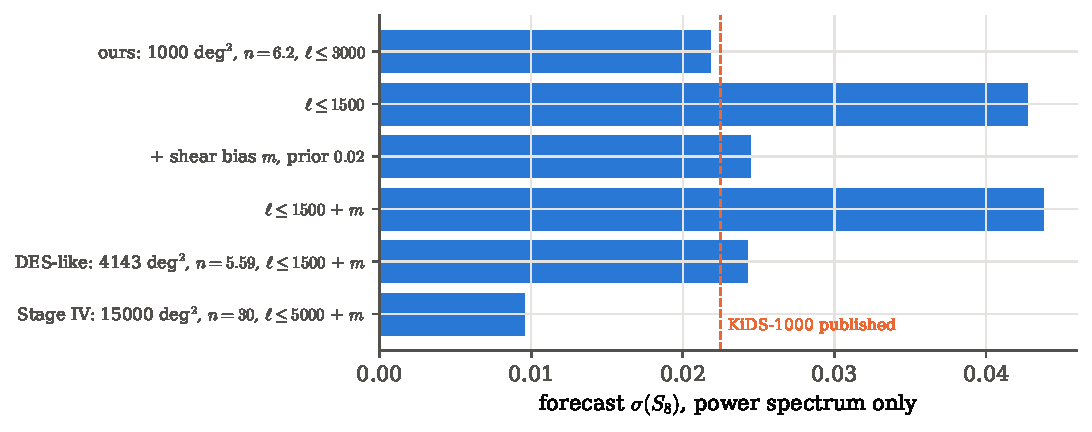
\includegraphics[width=0.85\linewidth]{figures/ch12/w_costs.pdf}
\caption{The forecast error on $S_8$ from the power spectrum alone, one source bin, Gaussian covariance, as the
survey and the nuisances change. A multiplicative shear bias with a $2\%$ prior, and a lower $\ell_{\max}$, each widen
the error; a Stage-IV survey with $30$ galaxies per arcmin$^2$ over $15\,000\,\mathrm{deg}^2$ narrows it, until the
prior on $m$ becomes the limit. The dashed line is the published KiDS-1000 precision, which uses five tomographic bins
and marginalises many more nuisances.}
\label{12w:fig:costs}
\end{figure}

\paragraph{Where the full version would go.} A Stage-IV survey, $15\,000\,\mathrm{deg}^2$ at $30$ galaxies per square
arcminute and $\ell\le5000$, reaches $\sigma(S_8)=\WCostSfour$ in the same forecast, with the $2\%$ prior on $m$; that
number is set mostly by the prior, which is why Stage-IV shear calibration must be ten times better. For the
higher-order summaries, the next step beyond our patch would be the same pipeline on HEALPix maps at
$N_{\rm side}=256$--$512$ cut from the Takahashi simulations, with the survey's mask and noise, a few hundred
covariance maps and an emulator over a few dozen cosmologies; at the cost of each simulation run, that is a cluster
project and not a laptop one.

\begin{inpractice}[The higher-order lensing analyses]
Peak counts have been measured in KiDS, DES and HSC data, and persistent homology, Minkowski functionals and
scattering transforms are being prepared for Stage-IV surveys, always with the same structure: summaries computed
identically on data and on $N$-body mocks that include the mask, the noise and the photometric redshifts; a
covariance from hundreds of independent mocks with the Hartlap or Sellentin--Heavens correction; an emulator of the
mean over a few dozen cosmologies; and an MCMC over cosmology and nuisances. The summaries themselves are the cheap
part, a second per map, as here; the simulations are the expensive part \cite{Kilbinger2015,Heydenreich2021}.
\end{inpractice}

Seen from the pipeline that runs through the whole book, from a physical model to a field, to a summary, to its
sampling distribution and to the parameters, the weak-lensing analysis is the same chain at every scale: research
spends its effort on the first link, realistic maps, and on the nuisances between the maps and the summaries, while the
statistics of the last two links (covariance, Hartlap, Fisher, MCMC) is what we built here and does not change.

\begin{recap}
\begin{itemize}[itemsep=1pt,leftmargin=1.2em]
  \item A shifted lognormal map $\kappa=\lambda[e^{G-s^2/2}-1]$ has the right spectrum and a floor at $-\lambda$, the
        empty beam; its reduced skewness is about $3/\lambda$, set by $\Omega_m$ and not by $\sigma_8$
        (\cref{12w:sec:lognormal}).
  \item Kaiser--Squires inversion is a rotation of each Fourier mode of the shear; it splits the map into $\kappa_E$
        and a $\kappa_B$ that should vanish. Shape noise enters both with power $\sigma_e^2/\bar n$; smoothing with a
        Gaussian of width $\theta_G$ leaves $\sigma_{\rm noise}^2=\sigma_e^2/(4\pi\theta_G^2\bar n)$, and a mask leaks
        $E$ into $B$ (\cref{12w:sec:ks}).
  \item The band powers of a $1000\,\mathrm{deg}^2$ KiDS-like survey measure $S_8$ to $\WLClSE$ in our lognormal
        forecast and leave $\Omega_m$ and $\sigma_8$ separately loose: a needle along $\sigma_8\Omega_m^{\alpha}=$ const,
        which the real likelihood bends into a banana (\cref{12w:sec:twopoint}).
  \item Summaries without a formula need simulated means and covariances: the Hartlap factor for the inverse
        covariance, common random numbers for the derivatives, and the subtraction of the derivative-noise bias
        \eqref{12w:eq:fisher-bias}, without which a Gaussian control shows gains that cannot exist
        (\cref{12w:sec:mc-fisher}).
  \item On lognormal maps, peaks, Minkowski functionals, Betti curves and persistent Betti numbers each add to the
        power spectrum, all together multiplying the figure of merit by $\WLAllGain$; on Gaussian maps they add
        nothing (\cref{12w:sec:beyond-results}). Published peak gains are reproduced in kind; the persistence gain over
        peaks is not, because a lognormal map has the topology of a Gaussian one, relabelled
        \eqref{12w:eq:ln-monotone} (\cref{12w:sec:beyond-repro}).
  \item Research replaces each simplification: ray-traced $N$-body maps, PSF and shear calibration, photometric
        redshifts, masks, tomography, blinding, emulators and MCMC over the nuisances (\cref{12w:sec:research}).
\end{itemize}
\end{recap}
\providecommand{\CtEbZero}{}\renewcommand{\CtEbZero}{1.28125}
\providecommand{\CtEbOne}{}\renewcommand{\CtEbOne}{0.03125}
\providecommand{\CtEchi}{}\renewcommand{\CtEchi}{1.25000}
\providecommand{\CtHandChi}{}\renewcommand{\CtHandChi}{1.25000}
\providecommand{\CtHandbOne}{}\renewcommand{\CtHandbOne}{0.03125}
\providecommand{\CtSdbZero}{}\renewcommand{\CtSdbZero}{0.544}
\providecommand{\CtSdChi}{}\renewcommand{\CtSdChi}{0.586}
\providecommand{\CtCovbb}{}\renewcommand{\CtCovbb}{-0.0088}
\providecommand{\CtPbZeroTwo}{}\renewcommand{\CtPbZeroTwo}{0.1992}
\providecommand{\CtMaxbZero}{}\renewcommand{\CtMaxbZero}{4}
\providecommand{\CtMCbZero}{}\renewcommand{\CtMCbZero}{1.2818}
\providecommand{\CtMCbZeroSe}{}\renewcommand{\CtMCbZeroSe}{0.0017}
\providecommand{\CtMCbOne}{}\renewcommand{\CtMCbOne}{0.0314}
\providecommand{\CsTwinSame}{}\renewcommand{\CsTwinSame}{1.776\times10^{-16}}
\providecommand{\CsSkewU}{}\renewcommand{\CsSkewU}{0.936}
\providecommand{\CsSkewTwin}{}\renewcommand{\CsSkewTwin}{0.038}
\providecommand{\CsPkRatio}{}\renewcommand{\CsPkRatio}{7.0}
\providecommand{\CsPkErr}{}\renewcommand{\CsPkErr}{3.2}
\providecommand{\CsShiftOne}{}\renewcommand{\CsShiftOne}{0.27}
\providecommand{\CsShiftOneSe}{}\renewcommand{\CsShiftOneSe}{0.08}
\providecommand{\CsShiftMone}{}\renewcommand{\CsShiftMone}{0.67}
\providecommand{\CsShiftThree}{}\renewcommand{\CsShiftThree}{2.57}
\providecommand{\CsSdOne}{}\renewcommand{\CsSdOne}{12.7}
\providecommand{\CsChiOne}{}\renewcommand{\CsChiOne}{56.5}
\providecommand{\CsSlopeZero}{}\renewcommand{\CsSlopeZero}{4.29}
\providecommand{\CsSlopeOne}{}\renewcommand{\CsSlopeOne}{4.48}
\providecommand{\CsSlopeTwo}{}\renewcommand{\CsSlopeTwo}{5.19}
\providecommand{\CsLam}{}\renewcommand{\CsLam}{0.0204}
\providecommand{\CsCorrLen}{}\renewcommand{\CsCorrLen}{4.9}
\providecommand{\CsMatNu}{}\renewcommand{\CsMatNu}{-2.0}
\providecommand{\CsMatMC}{}\renewcommand{\CsMatMC}{83}
\providecommand{\CsMatMCse}{}\renewcommand{\CsMatMCse}{3}
\providecommand{\CsMatTh}{}\renewcommand{\CsMatTh}{82}
\providecommand{\CsMatAMaxMC}{}\renewcommand{\CsMatAMaxMC}{19}
\providecommand{\CsMatAMaxTh}{}\renewcommand{\CsMatAMaxTh}{16}
\providecommand{\CsMatRatio}{}\renewcommand{\CsMatRatio}{0.19}
\providecommand{\CsGaussChiOne}{}\renewcommand{\CsGaussChiOne}{51.5}
\providecommand{\CsNseed}{}\renewcommand{\CsNseed}{400}
\providecommand{\CcNnull}{}\renewcommand{\CcNnull}{1000}
\providecommand{\CcNcheck}{}\renewcommand{\CcNcheck}{500}
\providecommand{\CcPb}{}\renewcommand{\CcPb}{26}
\providecommand{\CcTailb}{}\renewcommand{\CcTailb}{6.2}
\providecommand{\CcMaxb}{}\renewcommand{\CcMaxb}{1099}
\providecommand{\CcHartb}{}\renewcommand{\CcHartb}{0.973}
\providecommand{\CcRadj}{}\renewcommand{\CcRadj}{0.59}
\providecommand{\CcRcross}{}\renewcommand{\CcRcross}{0.40}
\providecommand{\CcMeanb}{}\renewcommand{\CcMeanb}{30.4}
\providecommand{\CcMeanbTh}{}\renewcommand{\CcMeanbTh}{26.7}
\providecommand{\CcPp}{}\renewcommand{\CcPp}{98}
\providecommand{\CcMeanp}{}\renewcommand{\CcMeanp}{113.1}
\providecommand{\CcMeanpTh}{}\renewcommand{\CcMeanpTh}{108.9}
\providecommand{\CcHartp}{}\renewcommand{\CcHartp}{0.901}
\providecommand{\CcPs}{}\renewcommand{\CcPs}{94}
\providecommand{\CcNs}{}\renewcommand{\CcNs}{150}
\providecommand{\CcMeans}{}\renewcommand{\CcMeans}{273}
\providecommand{\CcMeansTh}{}\renewcommand{\CcMeansTh}{261}
\providecommand{\CcHarts}{}\renewcommand{\CcHarts}{0.36}
\providecommand{\CcNmPb}{}\renewcommand{\CcNmPb}{974}
\providecommand{\CcNmPs}{}\renewcommand{\CcNmPs}{56}
\providecommand{\CcWidA}{}\renewcommand{\CcWidA}{0.036}
\providecommand{\CcWidB}{}\renewcommand{\CcWidB}{0.021}
\providecommand{\CcWidSum}{}\renewcommand{\CcWidSum}{0.057}
\providecommand{\CcWidRatio}{}\renewcommand{\CcWidRatio}{1.6}
\providecommand{\CcFaShort}{}\renewcommand{\CcFaShort}{100}
\providecommand{\CcFaHart}{}\renewcommand{\CcFaHart}{20}
\providecommand{\CcFaSim}{}\renewcommand{\CcFaSim}{6}
\providecommand{\CcFaHartX}{}\renewcommand{\CcFaHartX}{4}
\providecommand{\CcCalibKS}{}\renewcommand{\CcCalibKS}{0.11}
\providecommand{\CcCalibFive}{}\renewcommand{\CcCalibFive}{5.0}
\providecommand{\CcCalibFiveSd}{}\renewcommand{\CcCalibFiveSd}{1.4}
\providecommand{\CcCalibZ}{}\renewcommand{\CcCalibZ}{0.0}
\providecommand{\CcPt}{}\renewcommand{\CcPt}{22}
\providecommand{\CcRare}{}\renewcommand{\CcRare}{5}
\providecommand{\CcSqrtTwoP}{}\renewcommand{\CcSqrtTwoP}{7}
\providecommand{\CcCritT}{}\renewcommand{\CcCritT}{33.9}
\providecommand{\CcShiftT}{}\renewcommand{\CcShiftT}{11.9}
\providecommand{\CcOmniT}{}\renewcommand{\CcOmniT}{3.5}
\providecommand{\CcOmniRatio}{}\renewcommand{\CcOmniRatio}{1.8}
\providecommand{\CcSigT}{}\renewcommand{\CcSigT}{0.0141}
\providecommand{\CcEpsScore}{}\renewcommand{\CcEpsScore}{0.028}
\providecommand{\CcEpsOmni}{}\renewcommand{\CcEpsOmni}{0.049}
\providecommand{\CcCalibScoreFive}{}\renewcommand{\CcCalibScoreFive}{4.8}
\providecommand{\CcPowPkOmni}{}\renewcommand{\CcPowPkOmni}{4}
\providecommand{\CcPowPkScore}{}\renewcommand{\CcPowPkScore}{5}
\providecommand{\CcPowSkewFive}{}\renewcommand{\CcPowSkewFive}{22}
\providecommand{\CcPowAreaFive}{}\renewcommand{\CcPowAreaFive}{22}
\providecommand{\CcPowChiFive}{}\renewcommand{\CcPowChiFive}{95}
\providecommand{\CcPowBettiFive}{}\renewcommand{\CcPowBettiFive}{97}
\providecommand{\CcPowPdFive}{}\renewcommand{\CcPowPdFive}{92}
\providecommand{\CcPowBettiOmniFive}{}\renewcommand{\CcPowBettiOmniFive}{42}
\providecommand{\CcPowPdOmniFive}{}\renewcommand{\CcPowPdOmniFive}{19}
\providecommand{\CcPowBettiOmniTen}{}\renewcommand{\CcPowBettiOmniTen}{100}
\providecommand{\CcPowBettiTwo}{}\renewcommand{\CcPowBettiTwo}{54}
\providecommand{\CcPowBettiOmniTwo}{}\renewcommand{\CcPowBettiOmniTwo}{12}
\providecommand{\CcPowBettiAFive}{}\renewcommand{\CcPowBettiAFive}{7}
\providecommand{\CcPowBettiATen}{}\renewcommand{\CcPowBettiATen}{10}
\providecommand{\CcPowPdATen}{}\renewcommand{\CcPowPdATen}{9}
\providecommand{\CcPowBettiAOmniTen}{}\renewcommand{\CcPowBettiAOmniTen}{5}
\providecommand{\CcRespSkew}{}\renewcommand{\CcRespSkew}{27}
\providecommand{\CcRespArea}{}\renewcommand{\CcRespArea}{22}
\providecommand{\CcRespBz}{}\renewcommand{\CcRespBz}{27}
\providecommand{\CcRespBo}{}\renewcommand{\CcRespBo}{-26}
\providecommand{\CcCorrAreaTail}{}\renewcommand{\CcCorrAreaTail}{0.84}
\providecommand{\CcCorrAreaTwo}{}\renewcommand{\CcCorrAreaTwo}{0.41}
\providecommand{\CcCorrAreaSkew}{}\renewcommand{\CcCorrAreaSkew}{0.79}
\providecommand{\CcCorrBzTail}{}\renewcommand{\CcCorrBzTail}{0.32}
\providecommand{\CcCorrBzBo}{}\renewcommand{\CcCorrBzBo}{0.09}
\providecommand{\CcCorrBzSkew}{}\renewcommand{\CcCorrBzSkew}{0.36}
\providecommand{\CcOutBin}{}\renewcommand{\CcOutBin}{\beta_1(3)}
\providecommand{\CcOutVal}{}\renewcommand{\CcOutVal}{1}
\providecommand{\CcOutMean}{}\renewcommand{\CcOutMean}{0.00}
\providecommand{\CcOutSd}{}\renewcommand{\CcOutSd}{0.03}
\providecommand{\CcOutZ}{}\renewcommand{\CcOutZ}{32}
\providecommand{\CfSigPk}{}\renewcommand{\CfSigPk}{3.5}
\providecommand{\CfBiasPk}{}\renewcommand{\CfBiasPk}{1.52}
\providecommand{\CfSigSkew}{}\renewcommand{\CfSigSkew}{0.0365}
\providecommand{\CfSigArea}{}\renewcommand{\CfSigArea}{0.0364}
\providecommand{\CfSigChi}{}\renewcommand{\CfSigChi}{0.0145}
\providecommand{\CfSigBetti}{}\renewcommand{\CfSigBetti}{0.0139}
\providecommand{\CfSigPd}{}\renewcommand{\CfSigPd}{0.0133}
\providecommand{\CfSigBettiA}{}\renewcommand{\CfSigBettiA}{0.169}
\providecommand{\CfSigPdA}{}\renewcommand{\CfSigPdA}{0.104}
\providecommand{\CfPdAOverBettiA}{}\renewcommand{\CfPdAOverBettiA}{0.62}
\providecommand{\CfSigBettiSkew}{}\renewcommand{\CfSigBettiSkew}{0.0129}
\providecommand{\CfSigBettiPk}{}\renewcommand{\CfSigBettiPk}{0.0139}
\providecommand{\CfBiasBetti}{}\renewcommand{\CfBiasBetti}{0.1}
\providecommand{\CfBiasPd}{}\renewcommand{\CfBiasPd}{0.3}
\providecommand{\CfBiasPdA}{}\renewcommand{\CfBiasPdA}{3.7}
\providecommand{\CfStepA}{}\renewcommand{\CfStepA}{0.0138}
\providecommand{\CfStepB}{}\renewcommand{\CfStepB}{0.0139}
\providecommand{\CfStepC}{}\renewcommand{\CfStepC}{0.0147}
\providecommand{\CfSigInd}{}\renewcommand{\CfSigInd}{0.0138}
\providecommand{\CfBiasInd}{}\renewcommand{\CfBiasInd}{0}
\providecommand{\CfBiasCrn}{}\renewcommand{\CfBiasCrn}{0.1}
\providecommand{\CfP}{}\renewcommand{\CfP}{26}
\providecommand{\CfBiasEst}{}\renewcommand{\CfBiasEst}{21}
\providecommand{\CfFbetti}{}\renewcommand{\CfFbetti}{5182}
\providecommand{\CfBiasEstPct}{}\renewcommand{\CfBiasEstPct}{0.4}
\providecommand{\CfVarRatio}{}\renewcommand{\CfVarRatio}{62}
\providecommand{\CfRho}{}\renewcommand{\CfRho}{0.983}
\providecommand{\CfRhoFactor}{}\renewcommand{\CfRhoFactor}{61}
\providecommand{\CfConvA}{}\renewcommand{\CfConvA}{0.0135}
\providecommand{\CfConvB}{}\renewcommand{\CfConvB}{0.0135}
\providecommand{\CfConvC}{}\renewcommand{\CfConvC}{0.0139}
\providecommand{\CfConvD}{}\renewcommand{\CfConvD}{0.0140}
\providecommand{\CfConvE}{}\renewcommand{\CfConvE}{0.0139}
\providecommand{\CfFitRes}{}\renewcommand{\CfFitRes}{0.03}
\providecommand{\CfTrue}{}\renewcommand{\CfTrue}{0.05}
\providecommand{\CfGridMean}{}\renewcommand{\CfGridMean}{0.0364}
\providecommand{\CfGridSd}{}\renewcommand{\CfGridSd}{0.0148}
\providecommand{\CfGridLo}{}\renewcommand{\CfGridLo}{0.0216}
\providecommand{\CfGridHi}{}\renewcommand{\CfGridHi}{0.0509}
\providecommand{\CfMhMean}{}\renewcommand{\CfMhMean}{0.0361}
\providecommand{\CfMhSd}{}\renewcommand{\CfMhSd}{0.0147}
\providecommand{\CfMhAcc}{}\renewcommand{\CfMhAcc}{0.59}
\providecommand{\CfMhTau}{}\renewcommand{\CfMhTau}{5.5}
\providecommand{\CfMhNeff}{}\renewcommand{\CfMhNeff}{3400}
\providecommand{\CfEmMean}{}\renewcommand{\CfEmMean}{0.0368}
\providecommand{\CfEmSd}{}\renewcommand{\CfEmSd}{0.0144}
\providecommand{\CfMock}{}\renewcommand{\CfMock}{250}
\providecommand{\CfVarT}{}\renewcommand{\CfVarT}{1.15}
\providecommand{\CfCoverFive}{}\renewcommand{\CfCoverFive}{62}
\providecommand{\CfCoverZero}{}\renewcommand{\CfCoverZero}{72}
\providecommand{\CfZsdFive}{}\renewcommand{\CfZsdFive}{1.05}
\providecommand{\CfZmeanFive}{}\renewcommand{\CfZmeanFive}{0.16}
\providecommand{\CfZsdSe}{}\renewcommand{\CfZsdSe}{0.05}
\providecommand{\CfZmeanSe}{}\renewcommand{\CfZmeanSe}{0.07}
\providecommand{\CfVarTSe}{}\renewcommand{\CfVarTSe}{0.09}
\providecommand{\CfK}{}\renewcommand{\CfK}{1.070}
\providecommand{\CfKinv}{}\renewcommand{\CfKinv}{0.934}
\providecommand{\CfPhiK}{}\renewcommand{\CfPhiK}{0.825}
\providecommand{\CfCovK}{}\renewcommand{\CfCovK}{0.650}
\providecommand{\CfCovKPct}{}\renewcommand{\CfCovKPct}{65}
\providecommand{\CfKPct}{}\renewcommand{\CfKPct}{7}
\providecommand{\CfSdMedFive}{}\renewcommand{\CfSdMedFive}{0.0140}
\providecommand{\CfSdMedZero}{}\renewcommand{\CfSdMedZero}{0.0146}
\providecommand{\CpNside}{}\renewcommand{\CpNside}{128}
\providecommand{\CpLmax}{}\renewcommand{\CpLmax}{383}
\providecommand{\CpPixArcmin}{}\renewcommand{\CpPixArcmin}{27}
\providecommand{\CpTone}{}\renewcommand{\CpTone}{208}
\providecommand{\CpChkBad}{}\renewcommand{\CpChkBad}{0}
\providecommand{\CpChkN}{}\renewcommand{\CpChkN}{26}
\providecommand{\CpLamFourty}{}\renewcommand{\CpLamFourty}{6059}
\providecommand{\CpLamOneSixty}{}\renewcommand{\CpLamOneSixty}{307}
\providecommand{\CpPeakFourty}{}\renewcommand{\CpPeakFourty}{2556}
\providecommand{\CpPeakEighty}{}\renewcommand{\CpPeakEighty}{768}
\providecommand{\CpPeakOneSixty}{}\renewcommand{\CpPeakOneSixty}{163}
\providecommand{\CpRatioObs}{}\renewcommand{\CpRatioObs}{15.7}
\providecommand{\CpRatioLam}{}\renewcommand{\CpRatioLam}{19.8}
\providecommand{\CpChiOneEighty}{}\renewcommand{\CpChiOneEighty}{682}
\providecommand{\CpGkfOneEighty}{}\renewcommand{\CpGkfOneEighty}{752}
\providecommand{\CpChiOneFourty}{}\renewcommand{\CpChiOneFourty}{2327}
\providecommand{\CpGkfOneFourty}{}\renewcommand{\CpGkfOneFourty}{2932}
\providecommand{\CpNfeatZero}{}\renewcommand{\CpNfeatZero}{3897}
\providecommand{\CpNfeatTwenty}{}\renewcommand{\CpNfeatTwenty}{8880}
\providecommand{\CpNfeatFifty}{}\renewcommand{\CpNfeatFifty}{16143}
\providecommand{\CpNfeatFiftyS}{}\renewcommand{\CpNfeatFiftyS}{3555}
\providecommand{\CpShortZero}{}\renewcommand{\CpShortZero}{1119}
\providecommand{\CpShortTwenty}{}\renewcommand{\CpShortTwenty}{2985}
\providecommand{\CpShortFifty}{}\renewcommand{\CpShortFifty}{3004}
\providecommand{\CpShortFiftyS}{}\renewcommand{\CpShortFiftyS}{1307}
\providecommand{\CpHotOneZero}{}\renewcommand{\CpHotOneZero}{765}
\providecommand{\CpHotOneFifty}{}\renewcommand{\CpHotOneFifty}{3114}
\providecommand{\CpHotOneFiftyS}{}\renewcommand{\CpHotOneFiftyS}{568}
\providecommand{\CpFsky}{}\renewcommand{\CpFsky}{0.654}
\providecommand{\CpMaskRatio}{}\renewcommand{\CpMaskRatio}{0.687}
\providecommand{\CpNcov}{}\renewcommand{\CpNcov}{600}
\providecommand{\CpNref}{}\renewcommand{\CpNref}{400}
\providecommand{\CpP}{}\renewcommand{\CpP}{26}
\providecommand{\CpHart}{}\renewcommand{\CpHart}{0.955}
\providecommand{\CpCalib}{}\renewcommand{\CpCalib}{8.0}
\providecommand{\CpCalibN}{}\renewcommand{\CpCalibN}{200}
\providecommand{\CpCalibSd}{}\renewcommand{\CpCalibSd}{2.2}
\providecommand{\CpCalibKS}{}\renewcommand{\CpCalibKS}{0.07}
\providecommand{\CpNnull}{}\renewcommand{\CpNnull}{1000}
\providecommand{\CpNdata}{}\renewcommand{\CpNdata}{100}
\providecommand{\CpNrenorm}{}\renewcommand{\CpNrenorm}{100}
\providecommand{\CpMedTwo}{}\renewcommand{\CpMedTwo}{0.22}
\providecommand{\CpPowTwo}{}\renewcommand{\CpPowTwo}{14}
\providecommand{\CpPclMedTwo}{}\renewcommand{\CpPclMedTwo}{0.42}
\providecommand{\CpPclPowTwo}{}\renewcommand{\CpPclPowTwo}{9}
\providecommand{\CpPclPullMax}{}\renewcommand{\CpPclPullMax}{2.5}
\providecommand{\CpMedFive}{}\renewcommand{\CpMedFive}{0.007}
\providecommand{\CpPowFive}{}\renewcommand{\CpPowFive}{98}
\providecommand{\CpMedFifteen}{}\renewcommand{\CpMedFifteen}{0.002}
\providecommand{\CpPowFifteen}{}\renewcommand{\CpPowFifteen}{100}
\providecommand{\CpPclMedFive}{}\renewcommand{\CpPclMedFive}{0.46}
\providecommand{\CpPclPowFive}{}\renewcommand{\CpPclPowFive}{4}
\providecommand{\CpPclMedFifteen}{}\renewcommand{\CpPclMedFifteen}{0.29}
\providecommand{\CpPclPowFifteen}{}\renewcommand{\CpPclPowFifteen}{23}
\providecommand{\CpPdataG}{}\renewcommand{\CpPdataG}{0.97}
\providecommand{\CpPdataNG}{}\renewcommand{\CpPdataNG}{0.002}
\providecommand{\CpPdataNGfive}{}\renewcommand{\CpPdataNGfive}{0.01}
\providecommand{\CpGudhiN}{}\renewcommand{\CpGudhiN}{198}
\providecommand{\CpGudhiNg}{}\renewcommand{\CpGudhiNg}{198}
\providecommand{\CpGudhiDiff}{}\renewcommand{\CpGudhiDiff}{0.0e+00}
\providecommand{\CbN}{}\renewcommand{\CbN}{20000}
\providecommand{\CbKeep}{}\renewcommand{\CbKeep}{400}
\providecommand{\CbKeepPct}{}\renewcommand{\CbKeepPct}{2}
\providecommand{\CbTobs}{}\renewcommand{\CbTobs}{0.0338}
\providecommand{\CbTol}{}\renewcommand{\CbTol}{0.0028}
\providecommand{\CbMeanT}{}\renewcommand{\CbMeanT}{0.0351}
\providecommand{\CbSdT}{}\renewcommand{\CbSdT}{0.0144}
\providecommand{\CbMeanAll}{}\renewcommand{\CbMeanAll}{0.0377}
\providecommand{\CbSdAll}{}\renewcommand{\CbSdAll}{0.0236}
\providecommand{\CbMeanL}{}\renewcommand{\CbMeanL}{0.0364}
\providecommand{\CbSdL}{}\renewcommand{\CbSdL}{0.0148}
\providecommand{\CbSlope}{}\renewcommand{\CbSlope}{0.92}
\providecommand{\CbScatter}{}\renewcommand{\CbScatter}{0.0163}
\providecommand{\CbSigF}{}\renewcommand{\CbSigF}{0.0140}
\providecommand{\CbScZero}{}\renewcommand{\CbScZero}{0.0136}
\providecommand{\CbScFive}{}\renewcommand{\CbScFive}{0.0143}
\providecommand{\CbDistTol}{}\renewcommand{\CbDistTol}{4.9}
\providecommand{\CbP}{}\renewcommand{\CbP}{26}
\providecommand{\CbNmaps}{}\renewcommand{\CbNmaps}{250}
\providecommand{\CbCover}{}\renewcommand{\CbCover}{65}
\providecommand{\CbCoverErr}{}\renewcommand{\CbCoverErr}{3}
\providecommand{\CbSdMed}{}\renewcommand{\CbSdMed}{0.0166}
\providecommand{\CrBZero}{}\renewcommand{\CrBZero}{0.0245}
\providecommand{\CrRelBZero}{}\renewcommand{\CrRelBZero}{1.76}
\providecommand{\CrThBZero}{}\renewcommand{\CrThBZero}{1.11}
\providecommand{\CrBOne}{}\renewcommand{\CrBOne}{0.0271}
\providecommand{\CrRelBOne}{}\renewcommand{\CrRelBOne}{1.95}
\providecommand{\CrThBOne}{}\renewcommand{\CrThBOne}{1.09}
\providecommand{\CrBBoth}{}\renewcommand{\CrBBoth}{0.0139}
\providecommand{\CrRelBBoth}{}\renewcommand{\CrRelBBoth}{1.00}
\providecommand{\CrThBBoth}{}\renewcommand{\CrThBBoth}{1.00}
\providecommand{\CrPZero}{}\renewcommand{\CrPZero}{0.0229}
\providecommand{\CrRelPZero}{}\renewcommand{\CrRelPZero}{1.65}
\providecommand{\CrThPZero}{}\renewcommand{\CrThPZero}{0.65}
\providecommand{\CrPOne}{}\renewcommand{\CrPOne}{0.0291}
\providecommand{\CrRelPOne}{}\renewcommand{\CrRelPOne}{2.10}
\providecommand{\CrThPOne}{}\renewcommand{\CrThPOne}{0.62}
\providecommand{\CrPBoth}{}\renewcommand{\CrPBoth}{0.0133}
\providecommand{\CrRelPBoth}{}\renewcommand{\CrRelPBoth}{0.96}
\providecommand{\CrThPBoth}{}\renewcommand{\CrThPBoth}{0.59}
\providecommand{\CrNormBZero}{}\renewcommand{\CrNormBZero}{0.0241}
\providecommand{\CrNormBOne}{}\renewcommand{\CrNormBOne}{0.0276}
\providecommand{\CrNormBBoth}{}\renewcommand{\CrNormBBoth}{0.0167}
\providecommand{\CrAnBZeroTwo}{}\renewcommand{\CrAnBZeroTwo}{4}
\providecommand{\CrTpBZeroTwo}{}\renewcommand{\CrTpBZeroTwo}{7}
\providecommand{\CrAnBZeroFive}{}\renewcommand{\CrAnBZeroFive}{12}
\providecommand{\CrTpBZeroFive}{}\renewcommand{\CrTpBZeroFive}{17}
\providecommand{\CrAnBOneTwo}{}\renewcommand{\CrAnBOneTwo}{8}
\providecommand{\CrTpBOneTwo}{}\renewcommand{\CrTpBOneTwo}{4}
\providecommand{\CrAnBOneFive}{}\renewcommand{\CrAnBOneFive}{12}
\providecommand{\CrTpBOneFive}{}\renewcommand{\CrTpBOneFive}{10}
\providecommand{\CrAnPZeroTwo}{}\renewcommand{\CrAnPZeroTwo}{4}
\providecommand{\CrTpPZeroTwo}{}\renewcommand{\CrTpPZeroTwo}{12}
\providecommand{\CrAnPZeroFive}{}\renewcommand{\CrAnPZeroFive}{6}
\providecommand{\CrTpPZeroFive}{}\renewcommand{\CrTpPZeroFive}{24}
\providecommand{\CrAnPOneTwo}{}\renewcommand{\CrAnPOneTwo}{9}
\providecommand{\CrTpPOneTwo}{}\renewcommand{\CrTpPOneTwo}{10}
\providecommand{\CrAnPOneFive}{}\renewcommand{\CrAnPOneFive}{14}
\providecommand{\CrTpPOneFive}{}\renewcommand{\CrTpPOneFive}{23}
\providecommand{\CrAnPkTwo}{}\renewcommand{\CrAnPkTwo}{3}
\providecommand{\CrTpPkTwo}{}\renewcommand{\CrTpPkTwo}{1}
\providecommand{\CrAnPkFive}{}\renewcommand{\CrAnPkFive}{3}
\providecommand{\CrTpPkFive}{}\renewcommand{\CrTpPkFive}{2}
\providecommand{\CrShiftBZero}{}\renewcommand{\CrShiftBZero}{2.0}
\providecommand{\CrPdOverNorm}{}\renewcommand{\CrPdOverNorm}{0.80}
\section{A topological summary is a random number}
\label{12c:sec:random}

In \cref{12a:sec:onemap} we took one Gaussian patch, coloured everything above a threshold, and counted: so many
pieces, so many holes, an Euler characteristic of so much. Run the same script with a different seed and every
one of those numbers changes. Nothing went wrong. A cosmological theory never predicts the map we observe; it
predicts the statistics of maps like it, and the sky hands us one draw. The counts we take from that draw are
therefore draws too. Counting pieces and holes did not take us out of probability. It gave us a new random
variable, and everything the earlier chapters built for random variables applies to it.

Write the parameters of the physical model as $\theta$ (for the moment one number, the amount of non-Gaussianity),
the random field the model produces as $\phi(\bm x;\theta)$, and the summary we compute from it, a Betti curve, an
Euler characteristic curve or a persistence diagram, as $S[\phi]$. Repeating the experiment, new field, same
recipe, gives a distribution of values,
\begin{equation}
  P(S\given\theta),
  \label{12c:eq:sampling}
\end{equation}
the \newterm{sampling distribution} of the summary. It is the bridge between topology and inference. Once we have
it, the ordinary questions return unchanged, and they can be said in words before any symbol:
\begin{enumerate}[itemsep=1pt]
  \item What values does the summary take, and how often, if the model with parameter $\theta$ is true?
  \item What is its average, how much does it scatter from map to map, and how does it co-vary with another summary
        computed from the same map?
  \item If the field were Gaussian, would a value like the one we measured, or one even further from the Gaussian
        average, be something we would reasonably expect?
  \item Which values of $\theta$ could have produced the value we measured, and how readily would each have
        produced it?
\end{enumerate}
The first two are prediction, the last two inference (\cref{ch:05}). Bayes' theorem connects them exactly as
before, $P(\theta\given S)\propto P(S\given\theta)\,P(\theta)$. Topology does not compete with Bayesian inference; it
supplies a representation of the data on which Bayesian inference can act. Two separate questions are in play, and
it helps to keep them apart. \emph{What should we measure}, because it has physical meaning or is robust to what
we consider nuisance? That is what \cref{12a:sec:nuisance,12b:sec:filtration} were about. \emph{How does the
uncertainty in what we measured become a statement about $\theta$?} That is Monte Carlo, covariance, likelihood,
Fisher matrix and Markov chain, the subject of \cref{ch:06,ch:09,ch:10}. In the pipeline of the book,
physical model $\to$ field $\to$ choose what matters $\to$ summary $\to$ sampling distribution $\to$ physics, the
previous parts built the first three arrows; here we walk the last two.

\begin{workdef}[sampling distribution of a summary]
The \newterm{sampling distribution} $P(S\given\theta)$ of a summary $S$ \unpack{a number or a vector of numbers
computed from one map, such as $\beta_0$ at thirteen thresholds} is the distribution of the values of $S$ over
independent realisations of the field \unpack{new random phases and amplitudes, same model, same $\theta$}, each
passed through the same observation and the same computation.
\emph{Operational test:} simulate $n$ fields at $\theta$, compute $S$ on each, histogram; the mean, covariance and
quantiles of that sample estimate those of $P(S\given\theta)$ with errors that fall as $1/\sqrt n$.
\end{workdef}

\subsection{The smallest field: nine pixels}
\label{12c:sec:tiny}

Before any map, take a field small enough that we can list every realisation. A $3\times3$ grid of pixels; each
pixel is ``hot'' (above threshold) independently with probability $p$, and cold with probability $q=1-p$. This is
the excursion set of a field whose pixels are uncorrelated, at the threshold that leaves a fraction $p$ of them hot.
The hot set is the union of the closed hot squares, so two hot pixels that touch only at a corner belong to the same
piece, and a hole is a group of cold pixels, joined through shared sides, that cannot reach the outside of the grid
(the dual conventions of \cref{12a:sec:pixels}).

\paragraph{The question.} How many pieces $\beta_0$ and holes $\beta_1$ does the hot set have, and with what
probabilities? What is the average Euler characteristic $\chi=\beta_0-\beta_1$?

\paragraph{The average Euler characteristic, by hand.}
The pieces depend on how pixels connect, which makes $\beta_0$ awkward to average directly. The Euler characteristic
has a second form that never mentions connections: $\chi=V-E+F$ \eqref{12a:eq:vef}, where $F$ counts hot pixels, $E$
counts unit edges that belong to at least one hot pixel, and $V$ counts lattice points that belong to at least one
hot pixel. Each of $V$, $E$, $F$ is a sum of yes/no indicators, one per cell of the grid, and the average of a sum is
the sum of the averages whether or not the terms are independent. So we only need, for each cell, the probability that
at least one of the pixels touching it is hot.

The $3\times3$ grid has $16$ lattice points and $24$ unit edges, and they come in kinds according to how many pixels
touch them (\cref{12c:fig:tiny-grid}). Of the $16$ points, the $4$ corners of the grid touch one pixel, the $8$ other
points on the boundary touch two, and the $4$ interior points touch four. Of the $24$ edges, the $12$ on the boundary
touch one pixel and the $12$ interior ones touch two. A cell touched by $m$ pixels is present unless all $m$ are cold,
which happens with probability $q^m$. Then
\begin{align}
  \E[\chi]
  &\eqby{1}\E[V]-\E[E]+\E[F]\nonumber\\
  &\eqby{2}\bigl[4(1-q)+8(1-q^2)+4(1-q^4)\bigr]-\bigl[12(1-q)+12(1-q^2)\bigr]+9p\nonumber\\
  &\eqby{3}\bigl[4p+12-8q^2-4q^4\bigr]-\bigl[12p+12-12q^2\bigr]+9p\nonumber\\
  &\eqby{4}p+4q^2-4q^4 .
  \label{12c:eq:tiny-chi}
\end{align}
\begin{explain}
  \item Linearity of the expectation applied to $\chi=V-E+F$.
  \item Each kind of cell contributes (number of such cells)$\times\Prob(\text{not all of its pixels are cold})$; a
        pixel is hot with probability $p$, so $\E[F]=9p$.
  \item $1-q=p$ turns $4(1-q)$ into $4p$ and $12(1-q)$ into $12p$; the other brackets expand as $8(1-q^2)=8-8q^2$,
        $4(1-q^4)=4-4q^4$ and $12(1-q^2)=12-12q^2$.
  \item The constants cancel, $12-12=0$; the $p$ terms give $4p-12p+9p=p$; the $q^2$ terms give $-8q^2+12q^2=4q^2$; and
        $-4q^4$ is left.
\end{explain}
Two quick checks. At $p=1$ (all hot) it gives $1$: one square, no hole. At $p=0$ it gives $4-4=0$: nothing there.

\paragraph{The average number of holes, by hand.}
A hole needs cold pixels that cannot reach the outside through shared sides. Every pixel except the centre lies on the
boundary of the grid and so touches the outside; the only candidate hole is the centre pixel. The centre is enclosed
when it is cold and its four side-neighbours are hot; those four touch each other at their corners, so they form one
piece that rings the centre. The corner pixels do not matter: a cold corner shares no side with the centre. Hence
\begin{align}
  \E[\beta_1]&=\Prob(\text{centre cold})\,\Prob(\text{four side-neighbours hot})=q\,p^4 ,\nonumber\\
  \E[\beta_0]&=\E[\chi]+\E[\beta_1]=p+4q^2-4q^4+p^4q .
  \label{12c:eq:tiny-b}
\end{align}

\begin{figure}[htbp]
\centering
\begin{tikzpicture}[scale=0.95]
  \begin{scope}
    \foreach \i in {0,1,2} \foreach \j in {0,1,2} \draw[black!40] (\i,\j) rectangle ++(1,1);
    \foreach \i in {0,1,2} {\draw[very thick,fibreorange] (\i,0)--(\i+1,0); \draw[very thick,fibreorange] (\i,3)--(\i+1,3);
                            \draw[very thick,fibreorange] (0,\i)--(0,\i+1); \draw[very thick,fibreorange] (3,\i)--(3,\i+1);}
    \foreach \i in {0,1,2} \foreach \k in {1,2} {\draw[very thick,formblue] (\i,\k)--(\i+1,\k); \draw[very thick,formblue] (\k,\i)--(\k,\i+1);}
    \foreach \x/\y in {0/0,3/0,0/3,3/3} \fill[bdryred] (\x,\y) circle (2.6pt);
    \foreach \x/\y in {1/0,2/0,1/3,2/3,0/1,0/2,3/1,3/2} \fill[tangentgreen] (\x,\y) circle (2.6pt);
    \foreach \x/\y in {1/1,2/1,1/2,2/2} \fill[black] (\x,\y) circle (2.6pt);
    \node[lbl,align=left,anchor=north west] at (-0.2,-0.25) {\textcolor{bdryred}{$\bullet$} 4 points, 1 pixel each\\
      \textcolor{tangentgreen}{$\bullet$} 8 points, 2 pixels each\\ $\bullet$ 4 points, 4 pixels each};
    \node[lbl,align=left,anchor=north west] at (-0.2,-1.75) {\textcolor{fibreorange}{\rule[0.5ex]{4mm}{1.2pt}} 12 edges, 1 pixel each\\
      \textcolor{formblue}{\rule[0.5ex]{4mm}{1.2pt}} 12 edges, 2 pixels each};
  \end{scope}
  \begin{scope}[xshift=5.2cm]
    \foreach \i in {0,1,2} \foreach \j in {0,1,2} \draw[black!40] (\i,\j) rectangle ++(1,1);
    \foreach \x/\y in {1/0,0/1,2/1,1/2} \fill[formblue!55] (\x,\y) rectangle ++(1,1);
    \foreach \x/\y in {1/0,0/1,2/1,1/2} \draw[black!40] (\x,\y) rectangle ++(1,1);
    \node[lbl] at (1.5,1.5) {cold};
    \foreach \x/\y in {0/0,2/0,0/2,2/2} \node[lbl,softgray] at (\x+0.5,\y+0.5) {any};
    \node[lbl,align=center,anchor=north] at (1.5,-0.25) {the one way to make a hole:\\ probability $q\,p^4$};
  \end{scope}
\end{tikzpicture}
\caption{The bookkeeping behind \eqref{12c:eq:tiny-chi} and \eqref{12c:eq:tiny-b}. Left: the $16$ lattice points and
$24$ edges of a $3\times3$ grid, sorted by how many pixels touch them; a cell is part of the hot set unless every pixel
touching it is cold. Right: the centre is the only pixel that cannot reach the outside, so the only hole is a cold
centre ringed by four hot side-neighbours; the corners can be anything.}
\label{12c:fig:tiny-grid}
\end{figure}

\paragraph{Example: the numbers at $p=\tfrac12$.} With $q=\tfrac12$, \eqref{12c:eq:tiny-chi} gives
$\E[\chi]=\tfrac12+4\cdot\tfrac14-4\cdot\tfrac1{16}=\tfrac12+1-\tfrac14=1.25$, and \eqref{12c:eq:tiny-b} gives
$\E[\beta_1]=\tfrac12\cdot\tfrac1{16}=\tfrac1{32}=0.03125$ and $\E[\beta_0]=1.28125$. The enumeration below gives
$\E[\chi]=\CtEchi$, $\E[\beta_1]=\CtEbOne$ and $\E[\beta_0]=\CtEbZero$.

\paragraph{Example: when are holes most common?} $\E[\beta_1]=p^4(1-p)$ is small at both ends: with few hot pixels
there is no ring, with many there is no cold centre. Setting the derivative to zero,
\begin{align*}
  \frac{\dd}{\dd p}\bigl[p^4(1-p)\bigr]
  \eqby{1}4p^3-5p^4
  \eqby{2}p^3(4-5p)=0
  \quad\Rightarrow\quad p=\tfrac45,\qquad \E[\beta_1]_{\max}=\bigl(\tfrac45\bigr)^4\tfrac15=0.082 .
\end{align*}
\begin{explain}
  \item Product rule: $\frac{\dd}{\dd p}p^4=4p^3$ and $\frac{\dd}{\dd p}(p^4\cdot p)=5p^4$.
  \item Factor out $p^3$; the root $p=0$ is the minimum.
\end{explain}
The holes peak when four fifths of the pixels are hot, as in the large maps of \cref{12a:sec:scan}, where holes
dominate below the median threshold and pieces above it.

\paragraph{Example: why at most four pieces?} Hot pixels that touch even at a corner are one piece, so separate pieces
need cold pixels between them in every direction. The four corner pixels can be hot and separate if everything else is
cold; a fifth hot pixel anywhere touches at least one of them or sits in the middle, which touches all four corners. So
$\beta_0\le4$, and the enumeration confirms that the largest value is $\CtMaxbZero$.

\paragraph{The whole distribution, and a Monte Carlo of it.}
The averages are not the whole story; we want $P(S\given p)$ itself. With nine pixels there are $2^9=512$
configurations, and each has probability $p^{k}q^{9-k}$ if $k$ of its pixels are hot. The script
\pyname{code/ch12/c01_tiny.py} lists all of them, counts pieces and holes with the from-scratch routines of
\cref{12a:sec:pixels}, adds up the probabilities, and checks every count against scikit-image:
\pyfile[firstline=29,lastline=41]{code/ch12/c01_tiny.py}{All 512 configurations of a $3\times3$ grid, counted twice}
\noindent The loop builds each configuration as a $3\times3$ boolean array, counts it with \pyname{betti_plane} and
\pyname{euler_cubical}, and asserts three things: the Euler relation $\chi=\beta_0-\beta_1$, the number of pieces
from scikit-image's \pyname{measure.label} with the 8-neighbour rule, and $\chi$ from its
\pyname{measure.euler_number}.
All $512\times3$ assertions pass. The last line stores, for each configuration, its counts and its number of hot
pixels, from which its probability follows.

Then, as we would have to for a real map, the script forgets the enumeration and draws $10^5$ random grids:
\pyfile[firstline=55,lastline=61]{code/ch12/c01_tiny.py}{The same distribution by Monte Carlo}
\noindent The Monte Carlo mean number of pieces is $\CtMCbZero\pm\CtMCbZeroSe$ against the exact $\CtEbZero$, and the
mean number of holes $\CtMCbOne$ against $\CtEbOne$. \Cref{12c:fig:tiny} shows the distribution of $\beta_0$ at
$p=\tfrac12$, exact and simulated side by side, and the three averages as functions of $p$.

\begin{figure}[htbp]
\centering
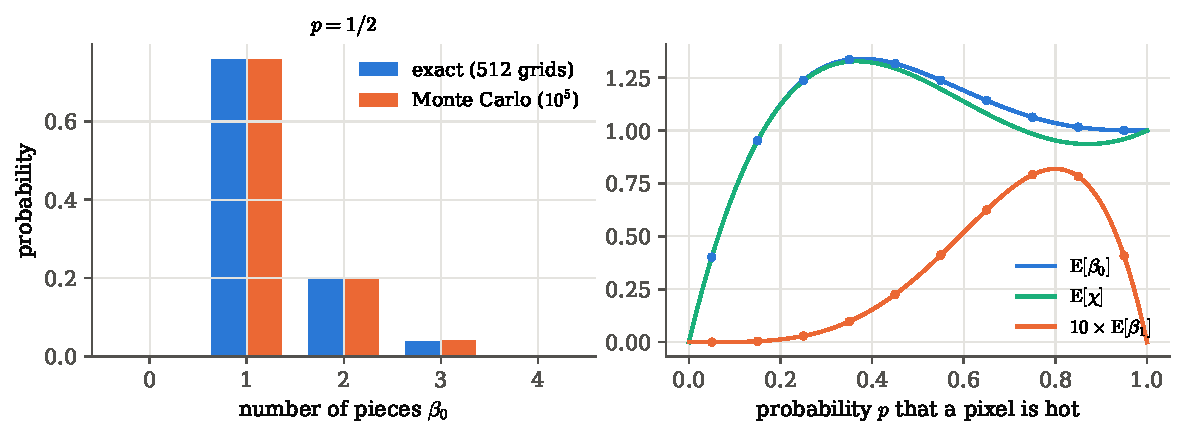
\includegraphics[width=\linewidth]{figures/ch12/c_tiny.pdf}
\caption{Left: the sampling distribution of the number of pieces on a $3\times3$ grid with $p=\frac12$, from all
$512$ configurations (blue) and from $10^5$ random grids (orange). One piece is by far the most common outcome; four,
the largest possible, almost never happens. Right: the averages \eqref{12c:eq:tiny-chi} and \eqref{12c:eq:tiny-b}
(lines) against exact enumeration at ten values of $p$ (dots); holes are multiplied by ten to be visible.}
\label{12c:fig:tiny}
\end{figure}

\paragraph{What the nine pixels already show.} Three things carry over to every real map. First, a count is a random
variable with a shape: at $p=\tfrac12$, $\Prob(\beta_0=2)=\CtPbZeroTwo$ and the standard deviations are
$\sigma(\beta_0)=\CtSdbZero$ and $\sigma(\chi)=\CtSdChi$, comparable to the means. Second, the counts of one map are
correlated with each other: $\Cov(\beta_0,\beta_1)=\CtCovbb$, negative because a hole needs the four side-pixels to be
hot, and four hot side-pixels make one piece out of what could have been several. A likelihood for a vector of counts
therefore needs a covariance matrix, not a list of variances. Third, enumeration stops working almost at once: a
$256\times256$ map has $2^{65536}$ binary configurations, and its pixels are correlated. What remains is the second
route, simulation, whose error falls as $1/\sqrt n$ with the number of maps whatever the size of the map
(\cref{6b:sec:sqrtN}). That route, followed all the way to a posterior, is what the local model of non-Gaussianity needs next.
\section{Two fields with one power spectrum}
\label{12c:sec:twins}

A Gaussian field is fixed completely by its power spectrum (\cref{7a:sec:grf}). The moment a field is not
Gaussian, the spectrum stops being the whole story, and in \cref{7a:sec:phases} we saw two maps with identical
spectra that looked nothing alike. Primordial non-Gaussianity of the local type is the physical version of that
situation: inflation with more than one field can add to the Gaussian potential a small piece of its own square
(\eqref{T3a:eq:local}; see the cosmology notes for the physics). The square adds a little power, but the dominant
signature is in the shapes: high peaks become a little higher and more numerous than deep troughs, or the other way
round. To study that signature cleanly we want a family of fields, labelled by the amount of non-Gaussianity, whose
power spectrum is \emph{exactly} the same for every member. Then whatever separates them cannot have come from the
spectrum.

\paragraph{The question.} Can we build two random fields with the same power spectrum, one Gaussian and one not; and
if so, do the Euler characteristic and the Betti curves of \cref{12a:sec:excursion,12b:sec:betti-curve} tell them
apart on average?

\subsection{The model, and why its spectrum does not depend on $\epsilon$}
\label{12c:sec:model}

Start from a Gaussian field $g$ on an $N\times N$ periodic grid ($N=256$), with zero mean, unit variance per pixel and
power spectrum $S_g(k)\propto k^{-2}$: equal power in every octave of wavenumber, the flat-sky version of a
scale-invariant spectrum. Its correlation function $\xi(\bm r)=\langle g(\bm x)g(\bm x+\bm r)\rangle$ is the inverse
Fourier transform of $S_g$, and $\xi(\bm 0)=1$. The non-Gaussian field adds a quadratic piece,
\begin{equation}
  \phi=g+\epsilon\,(g^2-1),
  \label{12c:eq:local}
\end{equation}
which is the local model with $\epsilon=f_{\rm NL}\sigma_g$ in units where $g$ has unit variance; subtracting $1=\langle
g^2\rangle$ keeps the mean zero. How much power does the quadratic piece add? The power spectrum is the Fourier
transform of the correlation function (Wiener--Khinchin, \eqref{7a:eq:wk}), so we need the correlation of $\phi$ at two
points $\bm x$ and $\bm y$, with $g_x\equiv g(\bm x)$ and $\xi\equiv\xi(\bm x-\bm y)$:
\begin{align}
  \langle\phi_x\phi_y\rangle
  &\eqby{1}\langle g_xg_y\rangle+\epsilon\bigl[\langle g_x(g_y^2-1)\rangle+\langle(g_x^2-1)g_y\rangle\bigr]
   +\epsilon^2\langle(g_x^2-1)(g_y^2-1)\rangle\nonumber\\
  &\eqby{2}\xi+0+\epsilon^2\bigl[\langle g_x^2g_y^2\rangle-\langle g_x^2\rangle-\langle g_y^2\rangle+1\bigr]\nonumber\\
  &\eqby{3}\xi+\epsilon^2\bigl[(1\cdot1+2\xi^2)-1-1+1\bigr]
   \eqby{4}\xi+2\epsilon^2\xi^2 .
  \label{12c:eq:xi-phi}
\end{align}
\begin{explain}
  \item Multiply out $(g_x+\epsilon(g_x^2-1))(g_y+\epsilon(g_y^2-1))$.
  \item The middle terms are averages of an odd number of zero-mean Gaussian factors ($g_xg_y^2$ and $g_x$ alone),
        which vanish by symmetry $g\to-g$.
  \item Wick's theorem \eqref{7a:eq:wick} with the four factors $g_x,g_x,g_y,g_y$: the three pairings give
        $\langle g_x^2\rangle\langle g_y^2\rangle+2\langle g_xg_y\rangle^2=1+2\xi^2$; and $\langle g^2\rangle=1$.
  \item $1+2\xi^2-1-1+1=2\xi^2$.
\end{explain}
Fourier transforming, the spectrum of $\phi$ is $S_\phi=S_g+\epsilon^2S_{2}$, with $S_{2}$ the transform of
$2\xi^2$: positive, of second order in $\epsilon$, and with a shape of its own. We remove it with a fixed linear
filter. Every Fourier mode of $\phi$ is multiplied by $R_\epsilon(k)=\sqrt{S_g(k)/S_\phi(k)}$, and then by a Gaussian
smoothing $W(k)=e^{-k^2s^2/2}$ of $s=2$ pixels, which plays the role of a beam. A linear filter multiplies the power
in each mode by its squared modulus (the convolution theorem, \cref{7a:sec:convolution}), so the observed map
$u=W\,R_\epsilon\,\phi$ has the spectrum
\begin{equation}
  S_u(k)=W^2(k)\,R_\epsilon^2(k)\,S_\phi(k)=W^2(k)\,S_g(k)\qquad\text{for every }\epsilon .
  \label{12c:eq:same-spectrum}
\end{equation}
This is exact, because $\phi$ is a quadratic polynomial in $g$ and \eqref{12c:eq:xi-phi} has no higher terms. The
filter does one more thing we will need: it mixes neighbouring pixels, so $u$ is \emph{not} a pointwise function of a
Gaussian map, and relabelling the thresholds (\cref{12a:sec:monotone}) will not undo $\epsilon$ completely.

\begin{pitfall}[The same ensemble spectrum, not the same spectrum map by map]
$R_\epsilon$ equalises the \emph{average} power in each mode. Each individual map still has its own measured spectrum,
scattered around the average by cosmic variance (\cref{7b:sec:cosmic-variance}), and the scatter itself depends weakly
on $\epsilon$ through the four-point function. ``The power spectrum cannot tell them apart'' means: the estimated spectra
of the two families have the same mean, so a likelihood built on the spectrum has no derivative with respect to
$\epsilon$.
\end{pitfall}

\paragraph{Example: one map and its phase-randomised twin.} A stronger version of the same statement holds for a
single map. Take the Fourier transform of one $\epsilon=0.2$ map, keep every modulus, and replace every phase by a
random one (\pyname{randomise_phases} from \cref{7a:sec:phases}). The two maps have the same $|\tilde u_{\bm k}|$, and so
the same periodogram, to machine precision: the largest relative difference of the moduli is $\CsTwinSame$. Yet the
skewness of the pixel values, $\langle u^3\rangle/\sigma^3$, is $\CsSkewU$ for the original and $\CsSkewTwin$ for the
twin. Random phases make every pixel a sum of many independent contributions, which pushes it towards Gaussian (the
central limit theorem, \cref{ch:02}); the non-Gaussianity of the original lived entirely in how its phases were
aligned. \Cref{12c:fig:twin} shows the two maps and the spectra.

\begin{figure}[htbp]
\centering
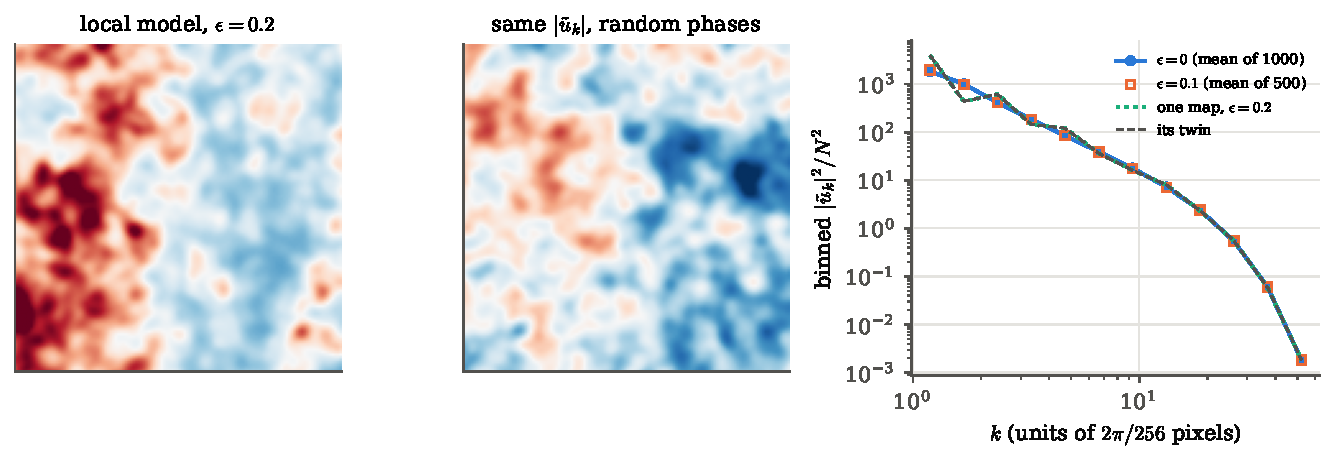
\includegraphics[width=\linewidth]{figures/ch12/c_twin.pdf}
\caption{Left: a quarter of one map of the local model with $\epsilon=0.2$ (red hot, blue cold), with sharp isolated hot
spots and broad shallow cold regions. Middle: the same Fourier moduli with random phases; the hot and cold sides look
alike. Right: binned spectra. The means over $1000$ maps at $\epsilon=0$ and $500$ at $\epsilon=0.1$ coincide, and the
single map and its twin coincide exactly.}
\label{12c:fig:twin}
\end{figure}

\paragraph{The ensembles.} The Monte Carlo behind every result below, \pyname{code/ch12/c02_mc_fnl.py}, draws three
sets of $256\times256$ maps: $1000$ maps at $\epsilon=0$ (the \emph{null} set, for means and covariances), $500$ more at
$\epsilon=0$ (the \emph{check} set, kept apart for calibrating tests), and $500$ seeds at each of
$\epsilon\in\{0,\pm0.025,\pm0.05,\pm0.1\}$ (the \emph{grid} set). In the grid set every value of $\epsilon$ of one seed is
built from the \emph{same} Gaussian field $g$, which will matter for derivatives (\cref{12c:sec:fisher}). For each map it
stores the binned periodogram, the skewness, the area fraction, $\chi$, $\beta_0$ and $\beta_1$ at the thirteen
thresholds $\nu=-3,-2.5,\dots,3$ (in units of the map's own standard deviation), the same three curves at
area-fraction thresholds $\nu_A$ \eqref{12a:eq:nuA}, and two-dimensional histograms of the persistence diagrams
(\cref{12b:sec:filtration}) computed with gudhi, whose diagrams agree exactly with our union--find
(\cref{12b:sec:checks}). The ensemble spectra at $\epsilon=0$ and $\epsilon=0.1$ differ by at most
$\CsPkRatio\%$ in any bin, against a Monte Carlo error of up to $\CsPkErr\%$ on one mean. The difference of two independent means
is noisier than either, and the worst of a dozen bins is expected near two standard errors: no sign of a difference.

\subsection{What the topology sees}
\label{12c:sec:shift}

With the spectrum out of the way, the question is whether the average curves move. Because each grid seed has its
own Gaussian $g$ for all values of $\epsilon$, the difference of a summary between $\epsilon=0.05$ and $\epsilon=0$ for the
same seed contains almost no cosmic variance, and $500$ seeds measure the mean shift precisely. \Cref{12c:fig:shift}
shows the result for $\chi$, $\beta_0$ and $\beta_1$.

\begin{figure}[htbp]
\centering
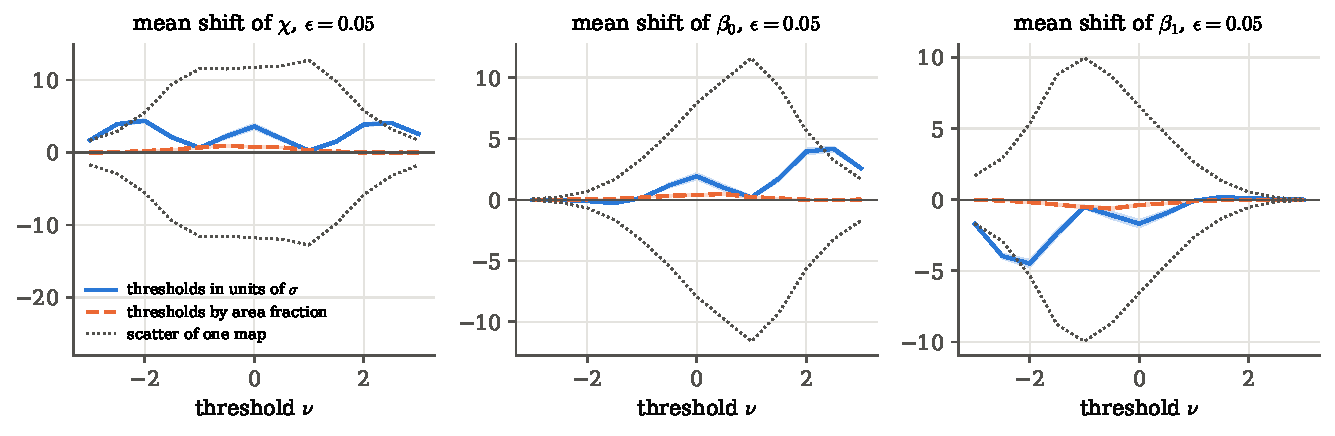
\includegraphics[width=\linewidth]{figures/ch12/c_shift.pdf}
\caption{Average change of the Euler characteristic and the Betti curves when $\epsilon$ goes from $0$ to $0.05$, from
$500$ pairs of maps that share their Gaussian field (bands: $\pm2$ standard errors). Solid: thresholds in units of the
map's $\sigma$; dashed: thresholds by area fraction. Dotted: the scatter of a single map at $\epsilon=0$. The extra hot
peaks show up in $\beta_0$ at high thresholds, the shallower cold regions as fewer lakes in $\beta_1$ at low ones.}
\label{12c:fig:shift}
\end{figure}

Three things are visible. The shift is real and has a shape: at $\nu=1$ the mean Euler characteristic moves by
$\CsShiftOne\pm\CsShiftOneSe$ (out of an average of $\CsChiOne$), at $\nu=-1$ by $\CsShiftMone$, and in the hot tail at
$\nu=3$ by $\CsShiftThree$. It is small compared with the scatter of one map at most thresholds ($\CsSdOne$ at $\nu=1$),
so no single threshold will detect $\epsilon=0.05$; but in the tails, where both the counts and their scatter are small,
the shift is a sizeable fraction of the scatter, and a vector of thresholds adds these pieces of evidence together, which
is the job of the covariance matrix (\cref{12c:sec:mc}). Finally, at area-fraction thresholds the shift almost disappears.
Most of what $\epsilon$ does to the counts is to move pixel values up or down, which is a relabelling of the threshold; what
survives at fixed area fraction is the part that comes from the smoothing mixing neighbours.

\subsection{Checking the shift against Matsubara's formula}
\label{12c:sec:matsubara}

For a weakly non-Gaussian field the first correction to the Euler characteristic is known
(\eqref{T3a:eq:matsubara}, from \cite{Matsubara2003}). In two dimensions, per unit area and with thresholds in units
of $\sigma_0$,
\begin{equation}
  \E[\chi(\nu)]=\frac{\lambda}{(2\pi)^{3/2}}\,e^{-\nu^2/2}\Bigl\{H_1(\nu)+\Bigl[\frac{S^{(0)}}{6}H_4(\nu)
  +\frac{2S^{(1)}}{3}H_2(\nu)+\frac{S^{(2)}}{3}\Bigr]\sigma_0\Bigr\},
  \label{12c:eq:mats}
\end{equation}
where $\lambda=\sigma_1^2/(2\sigma_0^2)$ is the gradient variance per component in units of the field variance
(\cref{12a:sec:gkf}), $H_n$ are the Hermite polynomials ($H_1=\nu$, $H_2=\nu^2-1$, $H_4=\nu^4-6\nu^2+3$), and
$S^{(0)}\sigma_0,S^{(1)}\sigma_0,S^{(2)}\sigma_0$ are the three skewness parameters \eqref{T3a:eq:skewpar}: the averages of
$u^3$, of $u^2\nabla^2u$ and of $|\nabla u|^2\nabla^2u$, suitably normalised. At $\epsilon=0$ the bracket vanishes and
we are back to \eqref{12a:eq:gkf2}.

\paragraph{The derivative with respect to $\epsilon$.} The three skewness parameters vanish at $\epsilon=0$ and grow in
proportion to $\epsilon$; write their slopes as $S_a'\equiv\dd(S^{(a)}\sigma_0)/\dd\epsilon$. For a map of area $A$,
differentiating \eqref{12c:eq:mats} at $\epsilon=0$ gives
\begin{equation}
  \frac{\dd\,\E[\chi(\nu)]}{\dd\epsilon}=\frac{A\lambda}{(2\pi)^{3/2}}\,e^{-\nu^2/2}
  \Bigl[\frac{S_0'}{6}H_4(\nu)+\frac{2S_1'}{3}H_2(\nu)+\frac{S_2'}{3}\Bigr] .
  \label{12c:eq:mats-deriv}
\end{equation}
For a pointwise distortion $u+\epsilon(u^2-1)$ all three slopes would be $6$ (\cref{T3a:sec:relabel}). The Monte Carlo script
\pyname{c02_mc_fnl.py} measures the three parameters on every grid map, and a straight-line fit in $\epsilon$ gives $S_0'=\CsSlopeZero$, $S_1'=\CsSlopeOne$, $S_2'=\CsSlopeTwo$: smaller than
$6$, because smoothing after squaring averages the square over neighbouring pixels, and unequal, because that averaging
treats the field and its derivatives differently.

\paragraph{The same derivative at fixed area fraction.} At area-fraction thresholds the term with $S^{(0)}$, the
one-point skewness, should drop out. Why, and what replaces it? The area fraction above $\nu$ is, to first order
(\eqref{T3a:eq:matsubara}, first line), $\Psi(\nu)+\varphi(\nu)\frac{S^{(0)}\sigma_0}{6}H_2(\nu)$, with $\Psi$ the Gaussian
tail probability \eqref{12a:eq:nuA} and $\varphi(\nu)=e^{-\nu^2/2}/\sqrt{2\pi}$ the Gaussian density. The threshold $\nu$
that encloses the area fraction $\Psi(\nu_A)$ therefore satisfies
\begin{align}
  \Psi(\nu_A)
  &\eqby{1}\Psi(\nu)+\varphi(\nu)\tfrac{S^{(0)}\sigma_0}{6}H_2(\nu)
   \eqby{2}\Psi(\nu_A)-\varphi(\nu_A)(\nu-\nu_A)+\varphi(\nu_A)\tfrac{S^{(0)}\sigma_0}{6}H_2(\nu_A)\nonumber\\
  &\Rightarrow\quad \nu=\nu_A+\tfrac{S^{(0)}\sigma_0}{6}H_2(\nu_A) .
  \label{12c:eq:nuA-shift}
\end{align}
\begin{explain}
  \item The definition of $\nu_A$: the measured area fraction at $\nu$ equals $\Psi(\nu_A)$.
  \item Taylor-expand $\Psi(\nu)$ around $\nu_A$ with $\Psi'=-\varphi$; in the correction term, which is already first
        order, replacing $\nu$ by $\nu_A$ changes only second-order terms.
\end{explain}
Now insert $\nu=\nu_A+\delta$ with $\delta=\frac{S^{(0)}\sigma_0}{6}H_2(\nu_A)$ into the Gaussian part of
\eqref{12c:eq:mats}, $e^{-\nu^2/2}H_1(\nu)$, and keep first order:
\begin{align}
  e^{-\nu^2/2}\nu
  &\eqby{1}e^{-\nu_A^2/2}\nu_A+\delta\,(1-\nu_A^2)\,e^{-\nu_A^2/2}
   \eqby{2}e^{-\nu_A^2/2}\Bigl[H_1-\frac{S^{(0)}\sigma_0}{6}H_2^2\Bigr]\nonumber\\
  &\eqby{3}e^{-\nu_A^2/2}\Bigl[H_1-\frac{S^{(0)}\sigma_0}{6}\bigl(H_4+4H_2+2\bigr)\Bigr] .
  \nonumber
\end{align}
\begin{explain}
  \item $\frac{\dd}{\dd\nu}(\nu e^{-\nu^2/2})=(1-\nu^2)e^{-\nu^2/2}$.
  \item $1-\nu_A^2=-H_2(\nu_A)$, and $\delta$ carries another $H_2$.
  \item $H_2^2=(\nu^2-1)^2=\nu^4-2\nu^2+1=H_4+4H_2+2$, all at $\nu_A$.
\end{explain}
The $H_4$ terms cancel against the $S^{(0)}H_4/6$ of \eqref{12c:eq:mats}, and the remaining $S^{(0)}$ terms combine with
the others:
\begin{equation}
  \frac{\dd\,\E[\chi(\nu_A)]}{\dd\epsilon}=\frac{A\lambda}{(2\pi)^{3/2}}\,e^{-\nu_A^2/2}
  \Bigl[\frac{2(S_1'-S_0')}{3}H_2(\nu_A)+\frac{S_2'-S_0'}{3}\Bigr] ,
  \label{12c:eq:mats-area}
\end{equation}
Matsubara's eq.~(3.54) in the variable $\nu_A$ \cite{Matsubara2003}. Only the differences between the slopes
of the three parameters survive: for the one-point skewness they carry no new information. For a pointwise distortion they vanish; for our smoothed field they are
$\CsSlopeOne-\CsSlopeZero$ and $\CsSlopeTwo-\CsSlopeZero$, small but not zero.

\paragraph{The comparison.} The formula is per unit area of a plane without edges, so the script
\pyname{code/ch12/c03_same_spectrum.py} uses periodic maps (the counting of \cref{12a:sec:vef} with wrap-around) and
$\CsNseed$ pairs at $\epsilon=\pm0.05$ that share $g$, and measures $\lambda=\CsLam$ per pixel$^2$ (a correlation length
$1/\sqrt{2\lambda}=\CsCorrLen$ pixels) on the maps themselves:
\pyfile[firstline=108,lastline=117]{code/ch12/c03_same_spectrum.py}{Matsubara's first-order prediction, at $\sigma$ and at area-fraction thresholds}
\noindent The first lines fit straight lines in $\epsilon$ to the skewness parameters measured on all grid maps (the
slopes $S_a'$) and take $\lambda$ from the $\epsilon=0$ maps; \pyname{amp} is
$A\lambda e^{-\nu^2/2}/(2\pi)^{3/2}$ with $A=N^2$ pixels; \pyname{pred} and \pyname{predA} are \eqref{12c:eq:mats-deriv} and
\eqref{12c:eq:mats-area}. \Cref{12c:fig:matsubara} compares them with the Monte Carlo. At $\nu=\CsMatNu$, where the
predicted derivative is largest, the simulation gives $\CsMatMC\pm\CsMatMCse$ and the formula $\CsMatTh$. At area-fraction
thresholds the derivative is at most $\CsMatAMaxMC$ (formula: $\CsMatAMaxTh$), about $\CsMatRatio$ of the $\sigma$-threshold
amplitude.

\begin{figure}[htbp]
\centering
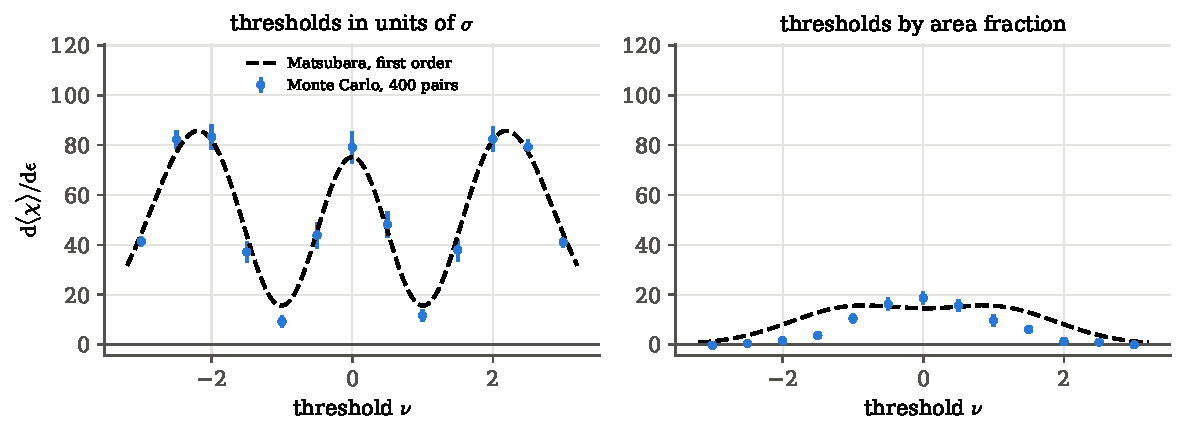
\includegraphics[width=0.92\linewidth]{figures/ch12/c_matsubara.pdf}
\caption{Derivative of the mean Euler characteristic of a periodic $256\times256$ map with respect to $\epsilon$. Points:
$\CsNseed$ pairs of maps at $\epsilon=\pm0.05$ sharing their Gaussian field ($\pm2$ standard errors). Dashed: Matsubara's
first-order formula with the skewness parameters measured on the maps. Left, thresholds in units of $\sigma$: the
$H_4$-dominated shape of a skewed histogram. Right, area-fraction thresholds: what is left is a small bump from the
non-local smoothing.}
\label{12c:fig:matsubara}
\end{figure}

The agreement says two things. The machinery is right: our counting, our maps and a perturbative formula derived by
other means meet within the Monte Carlo errors, apart from the thresholds $\nu=\pm1$ where both the Gaussian $\E\chi$
and its derivative change fastest across a pixel and the lattice effects of \cref{12a:sec:pixels} are largest. And the
physics is clear: most of the topological response to $\epsilon$ is a relabelling of the pixel values, and a smaller part,
about a fifth here, is in how the values are arranged. Both are invisible to the power spectrum.

\begin{keyidea}[Same spectrum, different shapes]
For the renormalised local model the power spectrum is the same for every $\epsilon$ \eqref{12c:eq:same-spectrum}, while the
mean Euler characteristic and Betti curves move in proportion to $\epsilon$, with the shape predicted by Matsubara's
formula. Any statistical power to detect $\epsilon$ in this family comes from beyond the two-point function.
\end{keyidea}
\section{The sampling distribution by simulation}
\label{12c:sec:mc}

Simulated covariances are not new to us. In \cref{8b:sec:nsims,8b:sec:hartlap} we estimated the covariance of masked
CMB band powers from simulated skies and derived why its inverse must be multiplied by $(n-p-2)/(n-1)$; in
\cref{12a:sec:planck} the same recipe gave the $36$-number $\chi^2$ of \textit{Planck}'s Minkowski-functional test on
Gaussian skies; and \cref{12w:sec:mc-fisher} used it for peak counts and Betti numbers of lensing maps. What is the same
here is the recipe: simulate the null model many times, average, form the covariance, invert, correct. What is new is the
use we make of it. In \cref{8b:sec:hartlap} the question was whether the \emph{average} of the inverse is right. To test a
hypothesis we need the whole \emph{distribution} of the $\chi^2$ of one map, including its tail, and our data vector is
made of counts, some of them small integers, which are not Gaussian at all.

\paragraph{The question.} If the field is Gaussian, what values does the $\chi^2$ of one map's Betti curves take, when
the mean and the covariance it is measured against were themselves estimated from a finite number of simulated maps?

\subsection{The data vector and its covariance}
\label{12c:sec:cov}

For each map the data vector stacks the two Betti curves of \cref{12c:sec:shift} at the thirteen thresholds,
$\bm S=(\beta_0(\nu_1),\dots,\beta_0(\nu_{13}),\beta_1(\nu_1),\dots,\beta_1(\nu_{13}))$. One entry, the number of lakes at
$\nu=3$, is zero in all but one of the simulated maps. An entry that never varied would carry no information and would make
the covariance singular, so such entries are dropped; this one varies, if only just, and stays,
leaving $p=\CcPb$ numbers. From the $n=\CcNnull$ null maps ($\epsilon=0$) we form the sample
mean and the sample covariance,
\begin{equation}
  \hat{\bm\mu}=\frac1n\sum_{i=1}^n\bm S_i,\qquad
  \hat\Cmat=\frac1{n-1}\sum_{i=1}^n(\bm S_i-\hat{\bm\mu})(\bm S_i-\hat{\bm\mu})\T ,
  \label{12c:eq:muC}
\end{equation}
exactly as in \cref{3a:sec:cov-noise}. \Cref{12c:fig:cov} shows the mean curves with the scatter of one map, and the
correlation matrix $\hat C_{ij}/\sqrt{\hat C_{ii}\hat C_{jj}}$.

\begin{figure}[htbp]
\centering
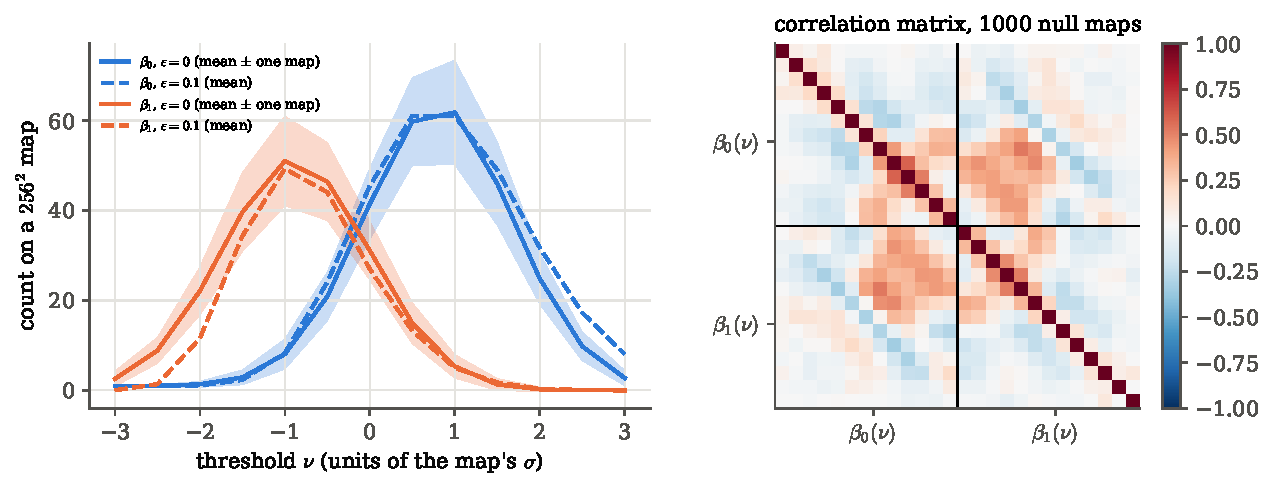
\includegraphics[width=\linewidth]{figures/ch12/c_cov.pdf}
\caption{Left: mean Betti curves of $1000$ Gaussian $256\times256$ maps (solid) with the $\pm1\sigma$ scatter of one map
(bands), and the mean at $\epsilon=0.1$ (dashed). Pieces ($\beta_0$) dominate above the median, lakes ($\beta_1$) below.
Right: the $\CcPb\times\CcPb$ correlation matrix of the counts. Neighbouring thresholds are positively correlated, and a broad
positive block links the hot pieces above the median to the lakes below it.}
\label{12c:fig:cov}
\end{figure}

\paragraph{Reading the correlation matrix.} Two structures stand out. Neighbouring thresholds are correlated, for example
$\CcRadj$ between $\beta_0(1)$ and $\beta_0(1.5)$, because they count largely the same islands: an island that is above
$1.5$ is also above $1$. And there is a positive correlation of $\CcRcross$ between the hot pieces at $\nu=1$ and the cold
lakes at $\nu=-1$, which never share a pixel. Why should they rise and fall together? Because both are counts of
features, and the number of features per unit area of a Gaussian field is set by one number, $\lambda=\sigma_1^2/2\sigma_0^2$
(\cref{12a:sec:gkf}). Thresholds are in units of each map's own standard deviation, and with equal power per octave a
good part of that standard deviation comes from the few longest waves in the box, which differ from map to map. A map whose
long waves happen to be weak has a smaller $\sigma_0$, the same small-scale roughness $\sigma_1$, a larger $\lambda$, and
therefore more islands \emph{and} more lakes at every threshold. Whatever the reason in a given case, the lesson of the
nine pixels returns: the counts of one map are not independent, and a likelihood must use the full matrix.

\paragraph{How many simulations?} Each entry of $\hat\Cmat$ is an average over $n$ maps, so its fractional error is
about $\sqrt{2/n}$, $4.5\%$ for $n=1000$; and the inverse is biased high by $(n-1)/(n-p-2)$, a factor $1/\CcHartb$ here
(\eqref{8b:eq:hartlap-derived}, \cite{Hartlap2007}). Hobson et al.\ make the same point in the language of the inverse
Wishart distribution: the covariance estimated from $n_s$ simulations is usable only if $n_s$ is well above twice the
length of the data vector \srcref{HobsonBMC}{\S3.4.3}. With $p=\CcPb$ and $n=\CcNnull$ we are far into the safe regime; with a
$\CcPp$-bin persistence histogram and $\CcNs$ maps we will not be.

\subsection{The $\chi^2$ of a new map when the covariance is estimated}
\label{12c:sec:hotelling}

Take one more map, independent of the $n$ simulations, and compute
\begin{equation}
  \chi^2=(\bm S-\hat{\bm\mu})\T\,\hat\Cmat^{-1}\,(\bm S-\hat{\bm\mu}) .
  \label{12c:eq:chi2}
\end{equation}
If $\hat{\bm\mu}$ and $\hat\Cmat$ were the true $\bm\mu$ and $\Cmat$, and $\bm S$ were Gaussian, this would be a sum of $p$
squared independent standard normal variables after whitening, a $\chi^2_p$ variable with mean $p$ (\cref{4a:sec:chi2-dist}).
Both estimates add noise. How much?

\paragraph{Its average.} Suppose $\bm S$ and the simulations are Gaussian with mean $\bm\mu$ and covariance $\Cmat$. Three
facts are needed: $\bm S$ is independent of the simulations; for Gaussian samples $\hat{\bm\mu}$ and $\hat\Cmat$ are
independent of each other (\cref{8b:sec:hartlap}); and $\hat{\bm\mu}$ has covariance $\Cmat/n$. Then
\begin{align}
  \E[\chi^2]
  &\eqby{1}\E\Bigl[\Tr\bigl(\hat\Cmat^{-1}(\bm S-\hat{\bm\mu})(\bm S-\hat{\bm\mu})\T\bigr)\Bigr]
   \eqby{2}\Tr\Bigl(\E\bigl[\hat\Cmat^{-1}\bigr]\;\E\bigl[(\bm S-\hat{\bm\mu})(\bm S-\hat{\bm\mu})\T\bigr]\Bigr)\nonumber\\
  &\eqby{3}\Tr\Bigl(\frac{n-1}{n-p-2}\,\Cmat^{-1}\;\Bigl(1+\frac1n\Bigr)\Cmat\Bigr)
   \eqby{4}p\,\Bigl(1+\frac1n\Bigr)\frac{n-1}{n-p-2} .
  \label{12c:eq:chi2-mean}
\end{align}
\begin{explain}
  \item A number is its own trace, and $\Tr(\bm a\T\mathsf M\bm a)=\Tr(\mathsf M\bm a\bm a\T)$.
  \item $\hat\Cmat$ is independent of both $\bm S$ and $\hat{\bm\mu}$, so the average of the product is the product of the
        averages; the trace is linear.
  \item The Hartlap result \eqref{8b:eq:hartlap-derived}; and $\bm S-\hat{\bm\mu}$ has mean zero and covariance
        $\Cmat+\Cmat/n$, because the two terms are independent and their covariances add.
  \item $\Tr(\Cmat^{-1}\Cmat)=\Tr\Id=p$.
\end{explain}
The factor $1+1/n$ comes from the noise in the mean, the factor $(n-1)/(n-p-2)$ from the noise in the covariance.

\paragraph{Its whole distribution.} The same ingredients give the shape. Whiten the problem: in coordinates where
$\Cmat=\Id$, the vector $\bm w=(\bm S-\hat{\bm\mu})/\sqrt{1+1/n}$ is a standard normal vector, so $|\bm w|^2\sim\chi^2_p$.
Now look at $\hat\Cmat^{-1}$ along the direction of $\bm w$. \Cref{8b:sec:hartlap} showed, through the Schur complement
\eqref{8b:eq:schur}, that the diagonal element of $(k\hat\Cmat)^{-1}$ along any fixed direction is one over a
$\chi^2_{k-p+1}$ variable when $\Cmat=\Id$, with $k=n-1$. In whitened coordinates the simulations look the same in every
direction, and they are independent of $\bm w$, so we may take the direction of $\bm w$ as the fixed one. Therefore
\begin{align}
  \chi^2
  &\eqby{1}\Bigl(1+\frac1n\Bigr)|\bm w|^2\;\hat{\bm e}\T\hat\Cmat^{-1}\hat{\bm e}
   \eqby{2}\Bigl(1+\frac1n\Bigr)(n-1)\,\frac{\chi^2_p}{\chi^2_{n-p}}
   \eqby{3}\Bigl(1+\frac1n\Bigr)\frac{(n-1)\,p}{n-p}\;F_{p,\,n-p},
  \label{12c:eq:hotelling}
\end{align}
\begin{explain}
  \item Write $\bm S-\hat{\bm\mu}=\sqrt{1+1/n}\,|\bm w|\,\hat{\bm e}$ with $\hat{\bm e}$ the unit vector along $\bm w$.
  \item $|\bm w|^2\sim\chi^2_p$; $\hat\Cmat=A/(n-1)$ with $A$ the scatter matrix of \cref{8b:sec:hartlap}, and
        $\hat{\bm e}\T A^{-1}\hat{\bm e}=1/\chi^2_{n-p}$ (the degrees of freedom $k-(p-1)=n-p$), independent of the numerator.
  \item The ratio $(\chi^2_p/p)/(\chi^2_{n-p}/(n-p))$ of two independent $\chi^2$ variables, each divided by its degrees of
        freedom, is Fisher's $F$ distribution with $(p,n-p)$ degrees of freedom.
\end{explain}
This is Hotelling's $T^2$ distribution, and its mean, $(n-p)/(n-p-2)$ for the $F$ factor, reproduces
\eqref{12c:eq:chi2-mean}. For $n\to\infty$ the denominator $\chi^2_{n-p}/(n-p)$ tends to one and $\chi^2_p$ returns.

\begin{keyidea}[A $\chi^2$ with a simulated covariance is wider than $\chi^2_p$]
If the mean and covariance of a Gaussian data vector of length $p$ are estimated from $n$ simulations, the $\chi^2$ of a new
independent vector is $(1+\frac1n)\frac{(n-1)p}{n-p}F_{p,n-p}$, with mean $p(1+\frac1n)\frac{n-1}{n-p-2}$. The Hartlap
factor fixes the mean; it does not fix the width, which comes from the $\chi^2_{n-p}$ in the denominator.
\end{keyidea}

\paragraph{How much wider?} The spread of a $\chi^2_k$ variable relative to its mean is $\sqrt{2k}/k=\sqrt{2/k}$, so the
logarithm of $\chi^2_k/k$ has a variance of about $2/k$ (the delta method: $\Var\ln X\approx\Var X/(\E X)^2$). The
logarithm of the ratio in \eqref{12c:eq:hotelling} is a difference of two independent such logarithms, so their variances
add:
\begin{equation}
  \Var\ln\chi^2\approx\frac2p+\frac2{n-p}\qquad\text{instead of}\qquad\frac2p .
  \label{12c:eq:width}
\end{equation}
For the Betti vector, $p=\CcPb$ and $n=\CcNnull$, the second term is $2/\CcNmPb$, negligible next to $2/\CcPb$. For a persistence
histogram with $p=\CcPs$ bins and only $n=\CcNs$ simulations it is $2/\CcNmPs=\CcWidA$ against $2/\CcPs=\CcWidB$: the $\chi^2$ is spread
$\sqrt{\CcWidSum/\CcWidB}\approx\CcWidRatio$ times wider, in the logarithm, than the $\chi^2_p$ table assumes, and no constant factor can
repair a wrong width.

\paragraph{The check.} The script \pyname{code/ch12/c04_test.py} computes \eqref{12c:eq:chi2} for the $\CcNcheck$ maps of the
check set against the mean and covariance of the $\CcNnull$ null maps:
\pyfile[firstline=55,lastline=70]{code/ch12/c04_test.py}{Mean, Hartlap-corrected inverse covariance, and the $\chi^2$ of new maps}
\noindent \pyname{fit} drops the entries that never change (and, if asked through \pyname{rare}, those that almost never
change; we use that in \cref{12c:sec:test}), estimates the mean and the covariance, inverts, and applies the Hartlap factor
if asked; \pyname{chi2} evaluates the quadratic form for a whole stack of maps at once with
\pyname{einsum}. For the Betti vector ($p=\CcPb$, $n=\CcNnull$) the average $\chi^2$ of the independent maps is
$\CcMeanb$, against $\CcMeanbTh$ from \eqref{12c:eq:chi2-mean}; a single map with a rare feature can move this average by a
few units, as the next paragraph shows. For the persistence histograms ($p=\CcPp$, $n=\CcNnull$) it
is $\CcMeanp$ against $\CcMeanpTh$. With only $n=\CcNs$ maps for the covariance ($p=\CcPs$) it is $\CcMeans$ against
$\CcMeansTh$; the Hartlap factor would be $\CcHarts$, and the $\chi^2_p$ table, centred at $\CcPs$, is not even in the right
place. \Cref{12c:fig:chi2} shows the three distributions.

\begin{figure}[htbp]
\centering
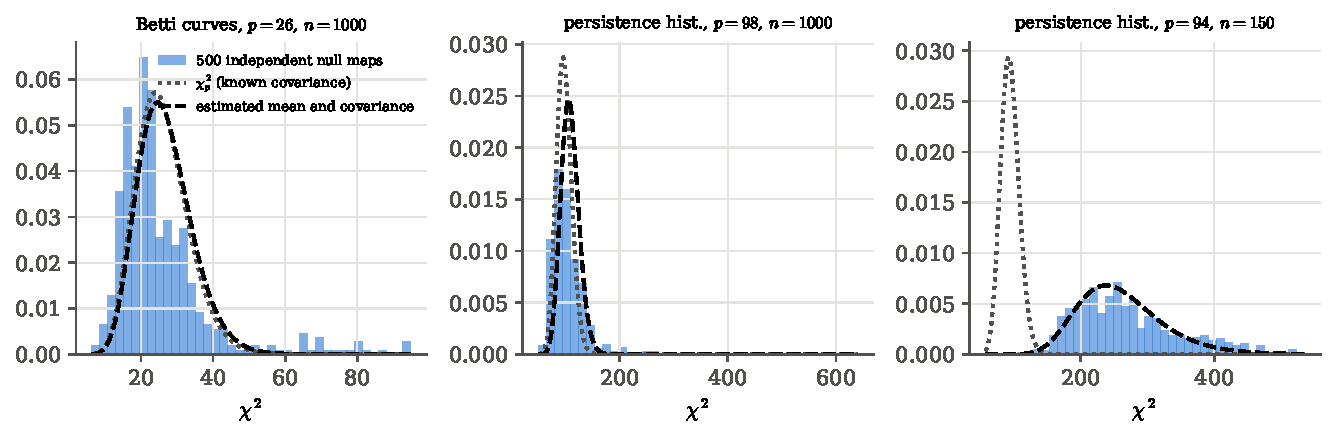
\includegraphics[width=\linewidth]{figures/ch12/c_chi2.pdf}
\caption{The $\chi^2$ \eqref{12c:eq:chi2} of $500$ Gaussian maps that were not used to estimate the mean and covariance
(histograms). Dotted: $\chi^2_p$, correct only if the covariance were known. Dashed: the Hotelling law
\eqref{12c:eq:hotelling}. Left, Betti curves with $1000$ simulations: the two curves nearly coincide. Middle, a
$\CcPp$-bin persistence histogram with $1000$ simulations: shifted and widened. Right, the same with $150$ simulations: the
$\chi^2_p$ curve is far off, the Hotelling law still follows the histogram.}
\label{12c:fig:chi2}
\end{figure}

\paragraph{Where the Gaussian assumption fails.} The derivation assumed Gaussian counts, and the bulk of the histograms
agrees with it. The tail does not. Of the $\CcNcheck$ Betti $\chi^2$ values, $\CcTailb\%$ lie above the $99.9$th
percentile of $\chi^2_{\CcPb}$, where $0.1\%$ were expected, and the largest is $\CcMaxb$. That one map is not exotic.
Its largest deviation is in $\CcOutBin$, a count whose simulated mean is $\CcOutMean$ with a scatter of only $\CcOutSd$; the
map had $\CcOutVal$, a deviation of $\CcOutZ$ standard deviations in one entry, and the square of that dominates the
$\chi^2$. Counts of rare features are small integers, closer to Poisson than to Gaussian, and a bin that is almost always
the same number has a tiny variance that turns an ordinary jump of one into an enormous $\chi^2$.

\begin{pitfall}[Rare-feature bins]
A bin that contains on average one or two features, or that almost never changes, makes the Gaussian $\chi^2$ heavy-tailed
and the covariance nearly singular. Either drop or merge such bins (Cole and Shiu discard bins whose fluctuations are not small
compared with their mean \cite{ColeShiu2018}), or keep them and take the distribution of the statistic from simulations
rather than from a table (\cref{12c:sec:simp}).
\end{pitfall}
\section{Is this map Gaussian? A test with a simulated null}
\label{12c:sec:test}

A colleague hands us one $256\times256$ map. Its power spectrum is exactly what a Gaussian field with spectrum $W^2S_g$
would have, so the spectrum says nothing. Was it drawn from the Gaussian model, $\epsilon=0$, or from one of its
non-Gaussian twins of \cref{12c:sec:model}? The Gaussian model has a special status: it is the hypothesis whose sampling
distribution we \emph{know}, because we can simulate it as often as we like. That is what makes it the null hypothesis
(\cref{4a:sec:null}): we do not try to prove the map is non-Gaussian; we ask whether ``it is just a Gaussian map, and what we
see happened by chance'' is a reasonable account of it.

\paragraph{The question.} If the map were Gaussian, would a $\chi^2$ of its Betti curves as large as the one we measured,
or larger, be something we would reasonably expect? And how often would the test catch a map that really has
$\epsilon=0.05$?

\subsection{A $p$-value from simulations}
\label{12c:sec:simp}

\Cref{12c:sec:hotelling} showed that the $\chi^2$ of a Gaussian map is not distributed as $\chi^2_p$, and that its tail is
heavier still because counts are not Gaussian. Instead of a formula we use simulations a second time. The check set of
\cref{12c:sec:model}, $N=\CcNcheck$ Gaussian maps that played no part in estimating $\hat{\bm\mu}$ and $\hat\Cmat$, gives
$N$ values $\chi^2_1,\dots,\chi^2_N$ of the statistic under the null hypothesis, computed exactly as for the observed map.
With $r$ the number of them at least as large as the observed $\chi^2_{\rm obs}$, define
\begin{equation}
  p=\frac{1+r}{1+N} .
  \label{12c:eq:psim}
\end{equation}

\paragraph{Why this is a valid $p$-value.} If the null hypothesis is true, the observed map is just one more Gaussian map:
its $\chi^2$ and the $N$ reference values are $N+1$ independent draws from the same continuous distribution. Then no draw is
special, and the observed one is equally likely to be the largest, the second largest, \ldots, the smallest. Write $R$ for
its rank counted from the top (the largest has $R=1$); $R=1+r$. For any $k=1,\dots,N+1$,
\begin{align}
  \Prob\Bigl(p\le\frac{k}{N+1}\Bigr)
  &\eqby{1}\Prob(1+r\le k)
   \eqby{2}\Prob(R\le k)
   \eqby{3}\frac{k}{N+1} .
  \label{12c:eq:psim-valid}
\end{align}
\begin{explain}
  \item Multiply both sides of $\frac{1+r}{N+1}\le\frac k{N+1}$ by $N+1$.
  \item $1+r$ is the rank from the top.
  \item Exchangeability: each of the $N+1$ ranks has probability $1/(N+1)$, and $k$ of them are $\le k$.
\end{explain}
So $\Prob(p\le\alpha)=\alpha$ whenever $\alpha$ is a multiple of $1/(N+1)$, and $\Prob(p\le\alpha)\le\alpha$ otherwise: a
$p$-value in the exact sense of \eqref{4a:eq:p-valid}, with no assumption about the shape of the distribution. The $+1$ in
numerator and denominator is not a fudge: it counts the observed map among the draws, and it keeps $p$ from ever being
zero. The smallest attainable value is $1/(N+1)=1/\CcNcheck$ here, so with $500$ reference maps no map can be called
more extreme than about $1$ in $500$.

\begin{workdef}[simulated $p$-value]
For a statistic $T$ whose distribution under $H_0$ can be simulated, draw $N$ independent realisations of $H_0$ through the
same pipeline as the data, compute $T_1,\dots,T_N$, and report $p=(1+\#\{T_i\ge T_{\rm obs}\})/(1+N)$
\unpack{the fraction of the $N+1$ values, the observed one included, that are at least as extreme}. It is exact for any $N$.
Its resolution is $1/(N+1)$.
\end{workdef}

\paragraph{Why the reference maps must be new.} It is tempting to reuse the $1000$ null maps for the reference
distribution. Their $\chi^2$ values against their own mean and covariance are systematically too small:
\begin{align}
  \sum_{i=1}^n(\bm S_i-\hat{\bm\mu})\T\hat\Cmat^{-1}(\bm S_i-\hat{\bm\mu})
  &\eqby{1}\Tr\Bigl(\hat\Cmat^{-1}\sum_{i=1}^n(\bm S_i-\hat{\bm\mu})(\bm S_i-\hat{\bm\mu})\T\Bigr)
   \eqby{2}\Tr\bigl(\hat\Cmat^{-1}(n-1)\hat\Cmat\bigr)
   \eqby{3}(n-1)\,p ,
  \nonumber
\end{align}
\begin{explain}
  \item The trace trick of \eqref{12c:eq:chi2-mean}, and the trace is linear.
  \item The definition \eqref{12c:eq:muC} of $\hat\Cmat$.
  \item $\Tr\Id=p$.
\end{explain}
so their average is $p(n-1)/n$, exactly and for every set of simulations, while a new map has the larger average
\eqref{12c:eq:chi2-mean}. The covariance was fitted to these very maps and ``explains'' them too well. A new map compared with
the in-sample distribution looks too extreme, and the test raises false alarms. The check set exists to avoid this; with a
single set of simulations one leaves each map out in turn, as the sphere analysis of \cref{12c:sec:sphere} does.

\subsection{Is the test honest?}
\label{12c:sec:calib}

Before using a test on data we run it on maps for which we know the answer. The $500$ grid seeds at $\epsilon=0$ are Gaussian
maps independent of both the null and the check set. Their $p$-values should be uniform between $0$ and $1$
(\cref{4a:sec:p-uniform}).

First, a choice the pitfall of \cref{12c:sec:hotelling} asked for. A bin in which almost every map has the same count, such as
the holes of the excursion set at $\nu=3$ or its pieces at $\nu=-3$, has a tiny variance, and one map with a single rare feature there gets an enormous $\chi^2$. Whether such
a bin enters the vector at all then depends on whether one of the $1000$ null maps happened to have the feature. For the tests
we drop every bin in which fewer than $\CcRare\%$ of the null maps differ from the median count. The Betti vector of the tests
has $p=\CcPt$ entries.

Now the check. $\CcCalibFive\%$ of the Gaussian maps get $p<0.05$, where $5\%$ were expected. How far off may that be? The
guarantee \eqref{12c:eq:psim-valid} is for one map and a reference set drawn afresh. Our $500$ maps all share the same $500$
reference values, so the noise of that one set moves every $p$-value together. Two uncertainties add: the binomial one of
$500$ maps, $\sqrt{0.05\times0.95/500}\approx1\%$, and the uncertainty of the $95$th percentile of $500$ reference values, about
the same size. Together they give $\CcCalibFiveSd\%$, so $\CcCalibFive\%$ is $\CcCalibZ$ standard deviations from $5\%$. For the
same reason a Kolmogorov--Smirnov test of the $p$-values against the uniform distribution would be wrong: it assumes independent
draws. The honest question is whether the $500$ values of $\chi^2$ and the $500$ reference values come from one distribution,
and the two-sample Kolmogorov--Smirnov test (\cref{4a:sec:ks}) answers it with $p=\CcCalibKS$.

\paragraph{Example: what goes wrong with a table.} Repeat the test with the persistence histograms and only $n=\CcNs$
simulations for the covariance, and compute the $p$-values of the same Gaussian maps in three ways. The $\chi^2_p$ table
with the raw $\hat\Cmat^{-1}$ rejects $\CcFaShort\%$ of these Gaussian maps at the $5\%$ level: the whole distribution sits
far to the right of the table (\cref{12c:fig:chi2}, right). Multiplying by the Hartlap factor puts the mean in the right
place, and the false alarm rate drops to $\CcFaHart\%$, still about $\CcFaHartX$ times too many: the distribution is too wide
\eqref{12c:eq:width}, and maps pile up at both ends of the $p$-value histogram. The simulated $p$-value \eqref{12c:eq:psim}
gives $\CcFaSim\%$. The left panel of \cref{12c:fig:power} shows the three histograms. When the mean and covariance are
estimated, the honest options are a likelihood that knows it (the $t$-distribution of Sellentin and Heavens, which
integrates over the unknown true covariance \cite{SellentinHeavens2016}) or a reference distribution from independent
simulations.

\subsection{How often does it catch $\epsilon\neq0$? Omnibus and aimed tests}
\label{12c:sec:power}

A test that never raises false alarms is useless if it never raises true ones. The power of a test is the probability that it
rejects $H_0$ when a specific alternative is true (\cref{4a:sec:power}). We measure it directly: compute the simulated
$p$-value for $250$ grid maps at each $\epsilon$ and count the fraction below $0.05$.

The $\chi^2$ test is an \newterm{omnibus} test: it asks whether the map is far from the Gaussian mean in \emph{any} of the
$p$ directions of the data vector. Local non-Gaussianity moves the mean in one particular direction, the derivative
$\bm d=\partial\bm\mu/\partial\epsilon$ that \cref{12c:fig:shift} showed. A test aimed at that direction should do better.

\paragraph{The aimed test is the score.} Model the summary as Gaussian with mean $\bm\mu(\epsilon)$ and a fixed covariance.
The log-likelihood is $\ln\Like(\epsilon)=-\frac12(\bm S-\bm\mu(\epsilon))\T\Cmat^{-1}(\bm S-\bm\mu(\epsilon))+$const, and its
slope at the null value $\epsilon=0$, the score of \cref{10a:sec:two-faces}, is
\begin{align}
  t\equiv\frac{\partial\ln\Like}{\partial\epsilon}\Big|_{\epsilon=0}
  &\eqby{1}-\tfrac12\Bigl[-\bm d\T\Cmat^{-1}(\bm S-\bm\mu_0)-(\bm S-\bm\mu_0)\T\Cmat^{-1}\bm d\Bigr]
   \eqby{2}\bm d\T\Cmat^{-1}(\bm S-\bm\mu_0) .
  \label{12c:eq:score}
\end{align}
\begin{explain}
  \item The product rule on the quadratic form; $\partial(\bm S-\bm\mu)/\partial\epsilon=-\bm d$, with $\bm\mu_0=\bm\mu(0)$.
  \item $\Cmat^{-1}$ is symmetric, so the two terms are equal.
\end{explain}
The score compresses the $p$ numbers into one, weighting each by how strongly it responds to $\epsilon$ and how noisy it is.
Under $H_0$ it has mean zero and variance $\bm d\T\Cmat^{-1}\Cmat\Cmat^{-1}\bm d=\bm d\T\Cmat^{-1}\bm d\equiv F$, the Fisher
information \eqref{10a:eq:gauss-fisher}. At a small $\epsilon$ its mean is $\bm d\T\Cmat^{-1}(\epsilon\bm d)=\epsilon F$, so
$t/\sqrt F$ is a unit normal shifted by $\epsilon\sqrt F$. By the Neyman--Pearson argument of \cref{4a:sec:np}, the one-sided test on $t$ is the most powerful
test of $\epsilon=0$ against a small positive $\epsilon$; since the sign of $\epsilon$ is not known in advance we use $|t|$. In practice $\bm d$ comes from the grid seeds $0$--$249$ and the power
is measured on seeds $250$--$499$, so that the direction is not tuned to the maps it is tested on.

\paragraph{Example: how much the aim is worth.} For the omnibus test write the whitened data as $\bm x=\bm z+\epsilon\Cmat^{-1/2}\bm d$
with $\bm z$ a standard normal vector; then $\chi^2=|\bm x|^2$ has mean
$\E|\bm z|^2+2\epsilon\,\E[\bm z]\T\Cmat^{-1/2}\bm d+\epsilon^2\bm d\T\Cmat^{-1}\bm d=p+\epsilon^2F$. Its null scatter is
$\sqrt{2p}$, so the shift has to compete with $\sqrt{2\cdot\CcPt}\approx\CcSqrtTwoP$ instead of $1$. At the $5\%$ level the score needs
$\epsilon\sqrt F\approx1.96$ for a $50\%$ chance of detection (two-sided, the far tail neglected). The omnibus test needs its
mean $\CcPt+\epsilon^2F$ to reach the $95$th percentile of $\chi^2_{\CcPt}$, $\CcCritT$, so $\epsilon^2F\approx\CcShiftT$ and
$\epsilon\sqrt F\approx\CcOmniT$: the omnibus test needs an $\epsilon$ about $\CcOmniRatio$ times larger. With the Fisher error of the
test's Betti vector, $F^{-1/2}=\CcSigT$ (\cref{12c:sec:fisher}), the score's $50\%$ point is $\epsilon\approx\CcEpsScore$ and the
measured power at $\epsilon=0.025$ is $\CcPowBettiTwo\%$; the omnibus test's estimated $50\%$ point is $\epsilon\approx\CcEpsOmni$,
and the measured powers are $\CcPowBettiOmniFive\%$ at $0.05$ and $\CcPowBettiOmniTen\%$ at $0.1$. Each measured power comes
from $250$ maps, so it is uncertain by a few per cent, and all of them lean on the same reference set and the same covariance.
The estimate ignores that the true null distribution is wider than $\chi^2_{\CcPt}$ (\cref{12c:sec:hotelling}), which lowers
the omnibus power.

\begin{figure}[htbp]
\centering
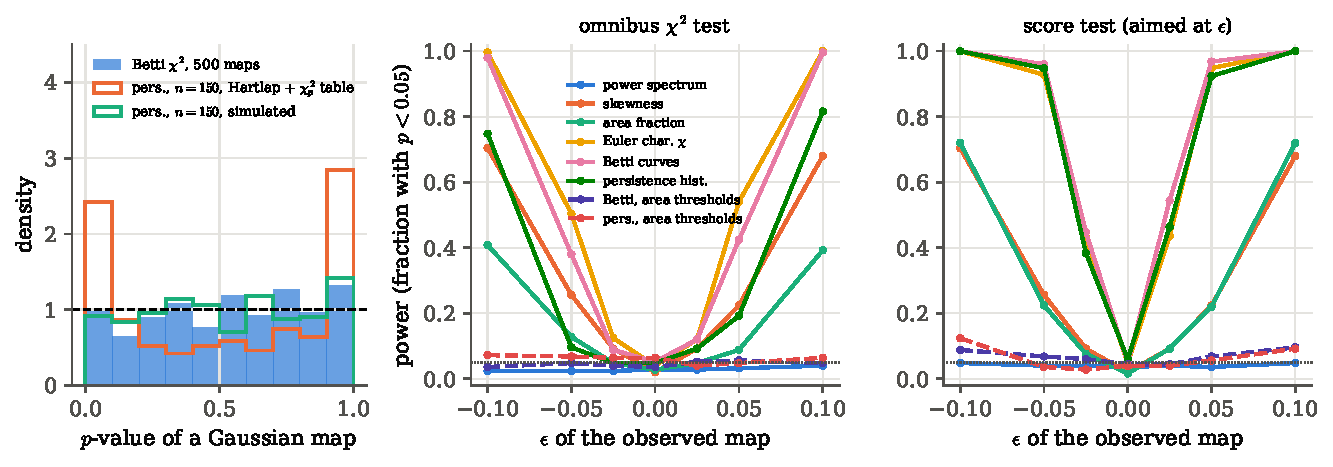
\includegraphics[width=\linewidth]{figures/ch12/c_power.pdf}
\caption{Left: $p$-values of Gaussian maps. Betti $\chi^2$ with a simulated reference (filled): flat within its noise, which is
larger than it looks because all $500$ maps share one reference set.
Persistence histogram with $150$ simulations, Hartlap-corrected $\chi^2$ referred to the $\chi^2_p$ table (orange): too many
small \emph{and} large values. The same with a simulated reference (green): flat. Middle and right: the fraction of maps
rejected at $p<0.05$ as a function of the true $\epsilon$, for the omnibus $\chi^2$ test and for the score test, for eight
summaries. Dashed: summaries at area-fraction thresholds. The power spectrum stays at the $5\%$ false-alarm level for every
$\epsilon$.}
\label{12c:fig:power}
\end{figure}

\paragraph{Which summary sees $\epsilon$?} \Cref{12c:fig:power} answers it for eight summaries. The power spectrum never
rises above the false-alarm rate (score test $\CcPowPkScore\%$ and omnibus $\CcPowPkOmni\%$ at $\epsilon=0.1$): by construction it
cannot. The one-point summaries see $\epsilon$, but weakly: at $\epsilon=0.05$ the score test on the skewness rejects
$\CcPowSkewFive\%$ of maps, on the area fractions $\CcPowAreaFive\%$. The topological summaries are far stronger: Euler
characteristic $\CcPowChiFive\%$, Betti curves $\CcPowBettiFive\%$, persistence histograms $\CcPowPdFive\%$. At area-fraction
thresholds the Betti curves drop to $\CcPowBettiAFive\%$ at $\epsilon=0.05$ and $\CcPowBettiATen\%$ at $0.1$.

\paragraph{Why do counts beat the skewness?} The last number says that most of what the Betti curves detect is the one-point
effect, values pushed up or down. Why then do they detect it so much better than the skewness, which measures exactly that? Look
at single entries. Per unit $\epsilon$, measured in units of its own map-to-map scatter, the skewness responds by $\CcRespSkew$,
the area fraction above $\nu=2.5$ by $\CcRespArea$, the number of pieces above $2.5$ by $\CcRespBz$ and the number of lakes
below $-2.5$ by $\CcRespBo$ (fewer lakes): all about the same size. The difference is in how much the entries repeat each other. The area fractions
above $2.5$ and above $3$ have a correlation of $\CcCorrAreaTail$ across maps, and the area fraction above $2.5$ is correlated
with the skewness at $\CcCorrAreaSkew$ and even with the area fraction below $-2.5$ at $\CcCorrAreaTwo$: they are moments of one
histogram, pulled by the same extreme pixels and the same normalisation. The number of pieces above $2.5$ and above $3$ correlate
at only $\CcCorrBzTail$, with the skewness at $\CcCorrBzSkew$, and the hot pieces above $2.5$ and the cold lakes below $-2.5$ at
$\CcCorrBzBo$: separate peaks in separate places are nearly independent witnesses. The Betti vector collects many such
witnesses, and the score test adds their evidence. The part of the signal that survives at fixed area fraction, the
arrangement of values rather than the values themselves, is real (\cref{12c:sec:matsubara}) but too weak for
one map: even at $\epsilon=0.1$ the score test on it rejects only $\CcPowBettiATen\%$ of the maps (Betti curves) and
$\CcPowPdATen\%$ (persistence histograms), against $5\%$ for Gaussian maps.

\begin{figure}[htbp]
\centering
\begin{tikzpicture}[
  bx/.style={draw=black!45,rounded corners=2pt,align=center,font=\small,text width=2.9cm,minimum height=1.05cm,fill=formblue!6},
  dt/.style={bx,fill=bdryred!6,draw=bdryred!60},
  arr/.style={->,thick,black!55}]
  \node[bx] (chk) at (0,0) {$500$ check maps\\ \scriptsize $\epsilon=0$, new seeds};
  \node[bx] (ref) at (3.8,0) {reference values\\ \scriptsize $\chi^2_1,\dots,\chi^2_{500}$};
  \node[bx] (null) at (0,-1.6) {$1000$ null maps\\ \scriptsize $\epsilon=0$};
  \node[bx] (fit) at (3.8,-1.6) {$\hat{\bm\mu}$, $\hat\Cmat^{-1}$\\ \scriptsize \eqref{12c:eq:muC}, Hartlap};
  \node[dt] (obs) at (0,-3.2) {observed map\\ \scriptsize unknown $\epsilon$};
  \node[dt] (cho) at (3.8,-3.2) {$\chi^2_{\rm obs}$\\ \scriptsize \eqref{12c:eq:chi2}};
  \node[dt,minimum height=3.6cm] (p) at (7.8,-1.6) {$p=\dfrac{1+r}{1+N}$\\ \scriptsize rank of $\chi^2_{\rm obs}$ among $N+1$};
  \draw[arr] (null) -- (fit);
  \draw[arr] (chk) -- (ref);
  \draw[arr] (obs) -- (cho);
  \draw[arr] (fit.north) -- (ref.south);
  \draw[arr] (fit.south) -- (cho.north);
  \draw[arr] (ref.east) -- (p.west |- ref.east);
  \draw[arr] (cho.east) -- (p.west |- cho.east);
\end{tikzpicture}
\caption{The test with a simulated null. One set of Gaussian maps (middle row) fixes the mean and the covariance, which every
$\chi^2$ uses; a second, independent set (top row) gives the distribution of the statistic under the null; the observed map
(bottom row) goes through exactly the same steps, and its
$p$-value is its rank among all of them. Every simulated quantity has its own map, so nothing is fitted to the maps it is
judged by.}
\label{12c:fig:testflow}
\end{figure}
\section{How well does one map measure $\epsilon$? A Fisher forecast}
\label{12c:sec:fisher}

A test answers yes or no. The next question is quantitative: if the map does have some $\epsilon$, how precisely can one map
measure it, and which summary measures it best? Before any data, the Fisher matrix answers this (\cref{ch:10}). For a data
vector that is Gaussian with mean $\bm\mu(\theta)$ and a covariance $\Cmat$ that we hold fixed, the Fisher information is the
mean part of \eqref{10a:eq:gauss-fisher}, and with one parameter it is a single number:
\begin{equation}
  F=\bm d\T\Cmat^{-1}\bm d,\qquad \bm d=\frac{\partial\bm\mu}{\partial\epsilon},\qquad \sigma(\epsilon)\ge F^{-1/2} .
  \label{12c:eq:fisher}
\end{equation}
It is the same number that set the score test's variance in \cref{12c:sec:power}: the Fisher information is how much the mean
moves, in units of the noise, per unit $\epsilon$. Two features of our problem need comment. There is no formula for $\bm d$; it is
estimated from simulations. And the full Gaussian Fisher matrix has a second term, $\frac12\Tr[\Cmat^{-1}\partial_\epsilon\Cmat\,
\Cmat^{-1}\partial_\epsilon\Cmat]$, from a covariance that changes with $\epsilon$. Holding $\Cmat$ at its $\epsilon=0$ value, as
almost every simulation-based analysis does, drops it; we return to what that costs in \cref{12c:sec:coverage}.

\paragraph{Derivatives from simulations, met before.} In \cref{12w:sec:mc-fisher} we estimated derivatives of peak counts and
Betti numbers of lensing maps with respect to $\Omega_m$ and $\sigma_8$ by central differences, with the same random numbers on
both sides of each difference (\emph{common random numbers}, \eqref{12w:eq:crn}), and we found that the noise in estimated
derivatives biases the Fisher matrix upwards by $\Tr[\Cmat^{-1}\bm\Sigma_d]/N_{\rm der}$ \eqref{12w:eq:fisher-bias}. There,
with two nearly degenerate parameters, that bias was dangerous. Here there is one parameter and no degeneracy, and the same
machinery is much better behaved, which is worth seeing in numbers.

\paragraph{The question.} What is $F^{-1/2}$ for each summary, and can we trust the estimate: does it depend on the step, on the
number of simulations, on whether the random numbers are shared?

\subsection{The derivative, seed by seed}
\label{12c:sec:deriv}

For each grid seed $k$ we have maps at $\epsilon=\pm h$ made from the same Gaussian field $g_k$. The per-seed central difference
and its average over $N_{\rm der}$ seeds are
\begin{equation}
  \bm D_k=\frac{\bm S_k(+h)-\bm S_k(-h)}{2h},\qquad \hat{\bm d}=\frac1{N_{\rm der}}\sum_{k=1}^{N_{\rm der}}\bm D_k .
  \label{12c:eq:Dk}
\end{equation}
Each $\bm S_k(\pm h)$ contains a large seed-specific part, the particular arrangement of peaks in $g_k$, and a small part that
responds to $\epsilon$. The difference removes the first and keeps the second (\cref{12c:fig:crn}).

\begin{figure}[htbp]
\centering
\begin{tikzpicture}
\begin{axis}[width=7.6cm,height=5.0cm,xmin=-0.13,xmax=0.13,ymin=36,ymax=64,
  xlabel={$\epsilon$},ylabel={$\beta_0(\nu)$ of one map},axis lines=left,
  xtick={-0.1,-0.05,0,0.05,0.1},scaled x ticks=false,xticklabel style={/pgf/number format/fixed},
  tick label style={font=\scriptsize},label style={font=\small},
  legend style={font=\scriptsize,draw=none,at={(1.02,0.5)},anchor=west}]
  \addplot[formblue,thick,domain=-0.12:0.12,samples=60] {58+40*x+0.6*sin(deg(90*x))};
  \addplot[fibreorange,thick,domain=-0.12:0.12,samples=60] {49+40*x-0.5*sin(deg(70*x))};
  \addplot[tangentgreen,thick,domain=-0.12:0.12,samples=60] {41+40*x+0.4*sin(deg(110*x))};
  \addplot[only marks,mark=*,mark size=1.6pt,black] coordinates
    {(-0.05,{58-2+0.6*sin(deg(-4.5))}) (0.05,{58+2+0.6*sin(deg(4.5))})
     (-0.05,{49-2-0.5*sin(deg(-3.5))}) (0.05,{49+2-0.5*sin(deg(3.5))})
     (-0.05,{41-2+0.4*sin(deg(-5.5))}) (0.05,{41+2+0.4*sin(deg(5.5))})};
  \addplot[bdryred,dashed,thick,domain=-0.12:0.12] {49+40*x};
  \legend{seed 1,seed 2,seed 3,,mean response}
\end{axis}
\end{tikzpicture}
\caption{Why common random numbers work. Each seed (one Gaussian field $g$) gives a count that depends on $\epsilon$; the three
seeds differ by far more than $\epsilon$ moves them, but their slopes are nearly the same. A difference taken along one seed (the
two dots on each curve, at $\epsilon=\pm h$) cancels the seed's offset and measures the slope; a difference between two seeds would
measure mostly the offsets.}
\label{12c:fig:crn}
\end{figure}

\paragraph{Example: how much the shared seed buys.} For one entry, the number of pieces at $\nu=1$, call $\sigma^2$ the variance of
$S_k(\pm h)$ across seeds and $\rho$ the correlation between $S_k(+h)$ and $S_k(-h)$ of the same seed. Then
\begin{align}
  \Var\bigl[S_k(+h)-S_k(-h)\bigr]
  &\eqby{1}\Var S_k(+h)+\Var S_k(-h)-2\Cov\bigl[S_k(+h),S_k(-h)\bigr]
   \eqby{2}2\sigma^2(1-\rho) ,
  \label{12c:eq:crn-var}
\end{align}
\begin{explain}
  \item The variance of a difference \eqref{12w:eq:crn}.
  \item Equal variances on both sides and $\Cov=\rho\sigma^2$.
\end{explain}
against $2\sigma^2$ for maps from different seeds. The measured correlation is $\rho=\CfRho$, so the shared seed reduces the
variance by $1/(1-\rho)\approx\CfRhoFactor$; the script measures the ratio directly as $\CfVarRatio$. One pair with shared random
numbers is worth about $\CfRhoFactor$ pairs without.

\subsection{Fisher errors for every summary}
\label{12c:sec:fisher-results}

The script \pyname{code/ch12/c05_fisher_post.py} does this for each summary:
\pyfile[firstline=56,lastline=78]{code/ch12/c05_fisher_post.py}{Fisher information with Monte Carlo derivatives, and its noise bias}
\noindent \pyname{null_model} gives the mean and the Hartlap-corrected inverse covariance from the $1000$ null maps.
\pyname{fisher} forms the per-seed differences \eqref{12c:eq:Dk}, either along a seed (\pyname{crn=True}) or between
different seeds, averages them, and returns $F=\hat{\bm d}\T\hat\Cmat^{-1}\hat{\bm d}$ together with the expected noise bias
$\Tr[\hat\Cmat^{-1}\bm\Sigma_d]/N_{\rm der}$, where \pyname{Sd} is the covariance of the per-seed derivatives divided by their
number.

\begin{figure}[htbp]
\centering
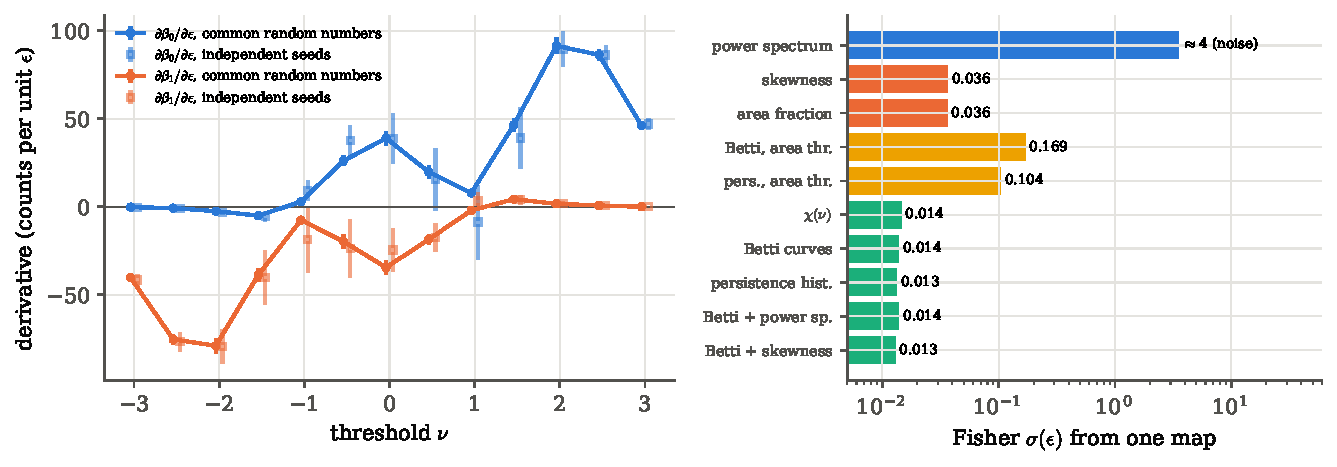
\includegraphics[width=\linewidth]{figures/ch12/c_fisher.pdf}
\caption{Left: the derivative of the Betti curves with respect to $\epsilon$ ($\pm2$ standard errors), from $500$ seeds with shared
random numbers (filled) and from $250$ pairs of different seeds (open): the same curve, with error bars several times smaller.
The response is concentrated in the tails, more pieces above $\nu\approx2$ and fewer lakes below $\nu\approx-2$. Right: the Fisher
error $F^{-1/2}$ on $\epsilon$ from one $256\times256$ map. Blue: power spectrum (no information, the bar is pure derivative noise);
orange: one-point summaries; yellow: topological summaries at area-fraction thresholds; green: topological summaries at
$\sigma$-thresholds and combinations.}
\label{12c:fig:fisher}
\end{figure}

\Cref{12c:fig:fisher} gives the results, with steps $h=0.05$ and $500$ seeds. The Euler characteristic gives $\sigma(\epsilon)=\CfSigChi$,
the Betti curves $\CfSigBetti$, the persistence histograms $\CfSigPd$. The skewness gives $\CfSigSkew$ and the area fractions
$\CfSigArea$, nearly three times worse; at area-fraction thresholds the Betti curves give $\CfSigBettiA$ and the persistence
histograms $\CfSigPdA$. These are the same rankings the tests of \cref{12c:fig:power} showed, now as error bars. Adding the
skewness to the Betti curves improves the error only to $\CfSigBettiSkew$: the Betti curves already contain most of what the
histogram of values knows. Adding the power spectrum changes nothing ($\CfSigBettiPk$).

\paragraph{Example: a Fisher error made of noise.} The power spectrum bar reads $\sigma(\epsilon)\approx\CfSigPk$, as if one map
could measure $\epsilon$ to within a few units. It cannot measure it at all: the true derivative is zero
\eqref{12c:eq:same-spectrum}. What the bar shows is \eqref{12w:eq:fisher-bias} with $\bm d=0$: the estimated $\hat{\bm d}$ is pure
noise, and $\hat{\bm d}\T\hat\Cmat^{-1}\hat{\bm d}$ is a positive number whose average is the noise term alone. The script's
estimate of that term is $\CfBiasPk$ times the measured $F$; a measured information equal to (or, within its own noise, below) its
expected noise bias is the signature of no information. For the topological summaries the same ratio is $\CfBiasBetti\%$ (Betti
curves), $\CfBiasPd\%$ (persistence histograms) and $\CfBiasPdA\%$ (persistence at area-fraction thresholds, where the signal is
weakest).

\paragraph{Example: why the noise bias is small here.} Even without shared seeds the Betti Fisher error is $\CfSigInd$ and the bias
below one per cent. Estimate it: without common random numbers, $\bm D_k$ has covariance about $2\Cmat/(2h)^2=200\,\Cmat$ for
$h=0.05$, so with $N_{\rm der}=250$ pairs
\begin{align*}
  \frac{\Tr[\Cmat^{-1}\bm\Sigma_d]}{N_{\rm der}}
  \eqby{1}\frac{\Tr[\Cmat^{-1}\,200\,\Cmat]}{250}
  \eqby{2}\frac{200\times\CfP}{250}\approx\CfBiasEst ,
\end{align*}
\begin{explain}
  \item The per-pair covariance $\bm\Sigma_d$: two independent maps, each with covariance $\Cmat$, difference divided by $2h=0.1$.
  \item $\Tr\Id=p=\CfP$.
\end{explain}
against $F=1/\CfSigBetti^2\approx\CfFbetti$: a $\CfBiasEstPct\%$ effect. The signal is strong, one parameter has no degeneracy to break, and noise in
the derivative cannot fake a direction the data do not have. In \cref{12w:sec:mc-fisher} the true information across the degeneracy
was a percent of the diagonal, and a bias of the same size changed the answer.

\paragraph{Checks on the derivative.} Three changes should not move a trustworthy number, and they do not. The step: with
$h=0.025$, $0.05$ and $0.1$ the Betti error is $\CfStepA$, $\CfStepB$ and $\CfStepC$; the largest step starts to feel the curvature
of $\bm\mu(\epsilon)$ (a central difference has an error of order $h^2\mu'''$, \cref{10a:sec:numderiv}). The number of seeds: with
$25$, $50$, $100$, $250$ and $500$ pairs it is $\CfConvA$, $\CfConvB$, $\CfConvC$, $\CfConvD$ and $\CfConvE$. And shared versus
independent seeds, $\CfSigBetti$ against $\CfSigInd$.

\paragraph{Verification and research with the same machinery.} \Cref{12c:sec:matsubara} used simulations to \emph{verify} a known result: Matsubara's perturbative formula for the mean Euler
characteristic. The Fisher errors above are \emph{research} numbers: no formula gives the covariance of Betti curves or the
response of a persistence histogram, and the simulated derivatives and covariance are the only route. The same split appears in
research. Cole and Shiu forecast $f_{\rm NL}$ from persistence diagrams of simulated CMB patches with exactly this construction,
a simulated mean at a few values of $f_{\rm NL}$ and a covariance from $2000$ Gaussian maps \cite{ColeShiu2018}; weak-lensing analyses
forecast $S_8$ from peaks and persistent Betti numbers in the same way, with emulators of the mean in place of finite differences
\cite{Heydenreich2021} (\cref{12w:sec:beyond}).
\section{From one map to a posterior for $\epsilon$}
\label{12c:sec:posterior}

The Fisher error is a forecast: the width the posterior will have on average, if the likelihood is Gaussian and the mean is
linear in the parameter. Now we take one map and compute the posterior itself. The reasoning is the one of parameter
estimation in \cref{ch:05}, applied to a new kind of data. The observed event is the Betti vector $\bm S_{\rm obs}$ of one map.
The candidate explanations are the values of $\epsilon$. For each candidate the likelihood asks how readily a map with that
$\epsilon$ would have produced these counts; Bayes' theorem combines the answers with a prior.

\paragraph{The question.} For one map with $\epsilon_{\rm true}=0.05$: which values of $\epsilon$ could have produced its Betti
curves, and how probable is each? And over many such maps, do the $68\%$ intervals we report contain the truth $68\%$ of the time?

\subsection{The likelihood}
\label{12c:sec:like}

We model the Betti vector as Gaussian, $\bm S\sim\Normal(\bm\mu(\epsilon),\Cmat)$. In the language of \cref{3b:sec:likelihood}, for a
given $\epsilon$ the model predicts the mean counts $\bm\mu(\epsilon)$; the observed counts differ from it by a fluctuation
$\bm S_{\rm obs}-\bm\mu(\epsilon)$; and the likelihood is the probability density of exactly that fluctuation under the map-to-map
scatter $\Cmat$:
\begin{equation}
  \ln\Like(\epsilon)=-\frac12\bigl(\bm S_{\rm obs}-\bm\mu(\epsilon)\bigr)\T\Cmat^{-1}\bigl(\bm S_{\rm obs}-\bm\mu(\epsilon)\bigr)+\text{const}.
  \label{12c:eq:like}
\end{equation}
A value of $\epsilon$ whose prediction requires an improbable fluctuation is disfavoured. Three ingredients have to be supplied,
and each comes from simulations.

\emph{The mean.} At the seven grid values of $\epsilon$ we average the Betti vectors of seeds $0$--$249$. A straight line through
them would miss the curvature that the step test of \cref{12c:sec:fisher-results} hinted at, so each of the $\CfP$ components is fitted
with a parabola in $\epsilon$. The largest misfit of any component at any grid point is $\CfFitRes$ of the scatter of one map: the
parabola is as good as the simulations can tell.

\emph{The covariance.} $\hat\Cmat$ from the $1000$ null maps, with the Hartlap factor, held fixed.

\emph{The prior.} Uniform on $|\epsilon|<0.15$, wide compared with the expected width and narrow enough that the parabola is
never extrapolated.

\begin{pitfall}[A Gaussian likelihood for counts is a model choice]
\eqref{12c:eq:like} is not derived from the physics; it is an approximation to $P(\bm S\given\epsilon)$ that is good when every
count is large and when $\Cmat$ hardly changes with $\epsilon$. Rare-feature bins violate the first (\cref{12c:sec:hotelling}), and
the coverage test below shows how the second fails. Replacing $\Cmat$ by $\Cmat(\epsilon)$ inside a Gaussian likelihood is not the
cure: for non-Gaussian data it adds a spurious term to the information and can make the posterior narrower than the Cram\'er--Rao
bound allows \cite{Carron2013}.
\end{pitfall}

\subsection{One map, three ways of computing its posterior}
\label{12c:sec:onemap}

The held-out seeds $250$--$499$ at $\epsilon=0.05$ serve as mock data. For the picture we take the first of them whose posterior
mean lies within one posterior standard deviation of the truth, a typical map, seed $\CfMock$; the coverage test below uses all
$250$. With one parameter the posterior can be computed on a grid of $1201$ values of $\epsilon$, which gives the reference answer.
The Metropolis sampler of \cref{9b:sec:code} and the ensemble sampler emcee (\cref{9b:sec:ensemble}) are then two independent
checks:
\pyfile[firstline=142,lastline=153]{code/ch12/c05_fisher_post.py}{The likelihood of the Betti vector, with a uniform prior}
\noindent \pyname{mu_of} evaluates the fitted parabolas, \pyname{loglike} returns \eqref{12c:eq:like} inside the prior and
$-\infty$ outside, which the samplers read as ``never accept''. The chain makes $20000$ steps with Gaussian proposals of width
$1.5$ times the grid posterior's standard deviation, somewhat narrower than the $2.38/\sqrt D=2.38$ standard deviations
that \cref{9b:sec:0234} found optimal for a Gaussian target; the price is a little efficiency, the chain accepting more
proposals than it would at the optimal width.

\begin{figure}[htbp]
\centering
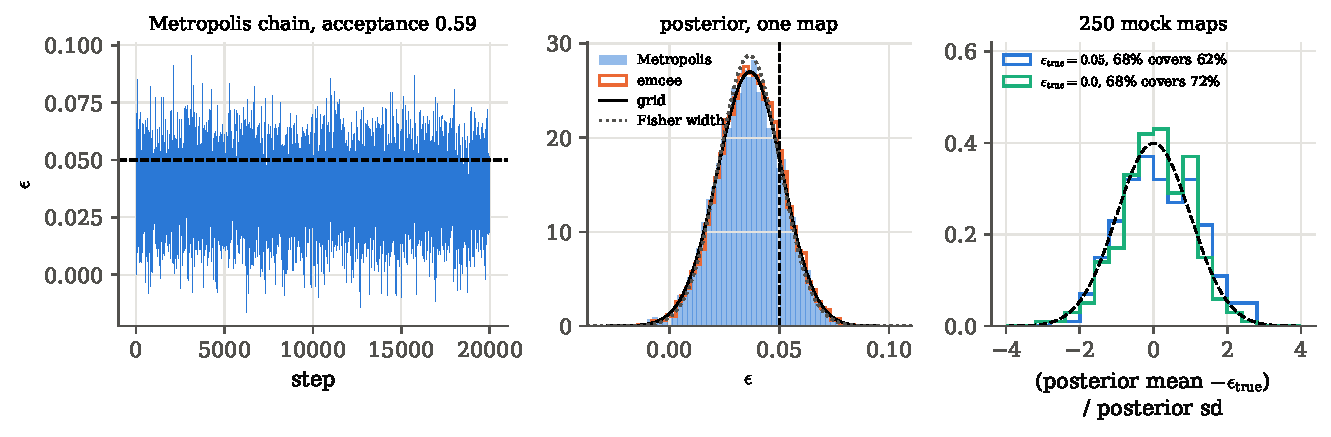
\includegraphics[width=\linewidth]{figures/ch12/c_post.pdf}
\caption{Left: the Metropolis chain for one map with $\epsilon_{\rm true}=0.05$ (dashed), well mixed from the first steps. Middle: its
histogram, the emcee histogram, the posterior on a grid and a Gaussian of the Fisher width centred on the grid mean: four curves
that lie on each other. Right: for $250$ maps, the distance of the posterior mean from the truth in units of the posterior
standard deviation, at $\epsilon_{\rm true}=0.05$ and $0$; dashed: the unit normal these should follow if the intervals are honest.}
\label{12c:fig:post}
\end{figure}

The grid posterior has mean $\CfGridMean$ and standard deviation $\CfGridSd$; its central $68\%$ interval is
$[\CfGridLo,\CfGridHi]$, which contains the true $\CfTrue$. The Metropolis chain gives $\CfMhMean\pm\CfMhSd$, with acceptance
fraction $\CfMhAcc$ and integrated autocorrelation time $\CfMhTau$ steps (\cref{9b:sec:tau}), so its $19000$ post-burn-in steps are
worth about $19000/\CfMhTau\approx\CfMhNeff$ independent draws, enough for a standard deviation good to about one per cent. emcee gives
$\CfEmMean\pm\CfEmSd$. The Fisher forecast was $\CfSigBetti$. Four routes, one answer: for this problem the likelihood is nearly Gaussian
in $\epsilon$ and the forecast is the posterior.

\subsection{Do the intervals cover?}
\label{12c:sec:coverage}

A $68\%$ credible interval is a statement about one map. Whether intervals constructed this way contain the truth in $68\%$ of
repeated experiments is a separate, frequentist property, \emph{coverage} (\cref{4b:sec:coverage}), and it can be tested only by
repeating the experiment, which simulations let us do. For each of the $250$ held-out maps at $\epsilon_{\rm true}=0.05$ we compute
the grid posterior and check whether its central $68\%$ interval contains $0.05$; then the same at $\epsilon_{\rm true}=0$.

At $\epsilon_{\rm true}=0$ the intervals contain the truth in $\CfCoverZero\%$ of maps; at $\epsilon_{\rm true}=0.05$ only in
$\CfCoverFive\%$. With $250$ maps the binomial uncertainty on such a fraction is $\sqrt{0.68\times0.32/250}=3\%$. The right panel
of \cref{12c:fig:post} shows the standardised errors $(\text{posterior mean}-\epsilon_{\rm true})/\text{posterior sd}$ at
$\epsilon_{\rm true}=0.05$: their standard deviation is $\CfZsdFive\pm\CfZsdSe$ instead of $1$, and their mean $\CfZmeanFive\pm\CfZmeanSe$
instead of $0$. With $250$ maps these numbers are themselves noisy, so they hint at a problem rather than prove one. Is there a
reason the posteriors should be too narrow at $\epsilon=0.05$?

\paragraph{What could make them too narrow?} Go through the ingredients one at a time. The prior is wide, so it cannot be it. The mean
$\bm\mu(\epsilon)$ was fitted at the very values of $\epsilon$ we test and fits to within $\CfFitRes$ of one map's scatter, so it is not
the mean. That leaves the covariance, which was measured at $\epsilon=0$ and used at every $\epsilon$. Is the scatter of the counts
larger at $\epsilon=0.05$? Project each map onto the direction that matters, the compressed statistic $t=\bm d\T\Cmat^{-1}\bm S$ of
\eqref{12c:eq:score}; its variance over the grid maps at $\epsilon=0.05$ is $\CfVarT\pm\CfVarTSe$ times its variance at $\epsilon=0$. Each seed gives
both maps from the same Gaussian field, so much of the noise cancels in this ratio, but not all: it sits above one by somewhat less
than two of its errors. That is a hint, not a proof, and it points the same way as the coverage. There is also a reason to expect it:
a positive $\epsilon$ makes the high peaks higher and more numerous, and counts of rarer, more extreme features fluctuate more. If
so, the likelihood underestimates the scatter by a factor $k=\sqrt{\CfVarT}\approx\CfK$ in exactly the direction that determines $\epsilon$.

\paragraph{Example: the coverage a wrong width produces.} Suppose the estimate $\hat\epsilon$ scatters around the truth with standard
deviation $k\sigma$ but we report $\hat\epsilon\pm\sigma$. The interval covers the truth when $|\hat\epsilon-\epsilon_{\rm true}|<\sigma$:
\begin{align}
  \Prob\bigl(|\hat\epsilon-\epsilon_{\rm true}|<\sigma\bigr)
  &\eqby{1}\Prob\Bigl(|Z|<\frac1k\Bigr)
   \eqby{2}2\Phi\Bigl(\frac1k\Bigr)-1
   \eqby{3}2\Phi(\CfKinv)-1
   \eqby{4}\CfCovK ,
  \label{12c:eq:coverage-k}
\end{align}
\begin{explain}
  \item Write $\hat\epsilon-\epsilon_{\rm true}=k\sigma Z$ with $Z$ a unit normal, and divide by $k\sigma$.
  \item $\Phi$ is the standard normal distribution function, and the normal is symmetric.
  \item $k=\sqrt{\CfVarT}=\CfK$.
  \item $\Phi(\CfKinv)=\CfPhiK$ from a table.
\end{explain}
A $\CfKPct\%$ error in the width turns a $68\%$ interval into a $\CfCovKPct\%$ one. The simulations found $\CfCoverFive\pm3\%$:
consistent with this cause, though $250$ maps cannot rule out others, such as the offset of the mean. At $\epsilon_{\rm true}=0$
the covariance is the right one, and the coverage, $\CfCoverZero\%$, agrees with $68\%$ within its uncertainty.

\begin{figure}[htbp]
\centering
\begin{tikzpicture}
\begin{axis}[width=8.2cm,height=5.0cm,xmin=0.78,xmax=1.62,ymin=0.44,ymax=0.96,
  xlabel={true scatter $/$ assumed width, $k$},ylabel={coverage of ``$68\%$''},
  axis lines=left,tick label style={font=\scriptsize},label style={font=\small},
  legend style={font=\scriptsize,draw=none,fill=none,at={(0.98,0.97)},anchor=north east}]
  \addplot[black,thick,smooth] coordinates {(0.80,0.7887) (0.85,0.7606) (0.90,0.7335) (0.95,0.7075) (1.00,0.6827)
    (1.05,0.6591) (1.10,0.6367) (1.15,0.6155) (1.20,0.5953) (1.25,0.5763) (1.30,0.5582) (1.35,0.5411) (1.40,0.5249)
    (1.45,0.5096) (1.50,0.4950) (1.55,0.4812) (1.60,0.4680)};
  \addlegendentry{$2\Phi(1/k)-1$}
  \addplot[only marks,mark=square*,mark size=2pt,fibreorange] coordinates {(\CfK,\CfCovK)};
  \addlegendentry{predicted from the variance ratio}
  \addplot[only marks,mark=*,mark size=2pt,formblue,error bars/.cd,y dir=both,y explicit]
    coordinates {(\CfZsdFive,{\CfCoverFive/100}) +- (0,0.03)};
  \addlegendentry{$250$ mock maps, $\epsilon_{\rm true}=0.05$}
  \draw[softgray,dashed] (axis cs:1,0.44) -- (axis cs:1,0.6827) -- (axis cs:0.78,0.6827);
\end{axis}
\end{tikzpicture}
\caption{The coverage of a nominal $68\%$ interval when the true scatter of the estimate is $k$ times the width we report,
\eqref{12c:eq:coverage-k}. Honest intervals sit at $k=1$ (dashed). The variance ratio measured for the compressed Betti statistic
predicts the orange square; the blue point is the coverage actually found over $250$ mock maps, placed at the measured spread of
their standardised errors, with its binomial error bar.}
\label{12c:fig:coverage}
\end{figure}

The remedy follows from the diagnosis. Measure the covariance near the answer rather than at an arbitrary fiducial point: after a
first pass, simulate the null set again at the best-fit $\epsilon$ and repeat. Or drop the Gaussian form altogether and let simulations
supply the likelihood, which is the subject of \cref{12c:sec:abc}. What we should not do is skip the test: coverage is the only check
that the error bars we publish mean what they say, and for a summary without a likelihood formula, simulations are the only way to
run it.
\section{The same experiment on the CMB sky}
\label{12c:sec:sphere}

A temperature map is a function on the celestial sphere, $T:S^2\to\R$, and we never see it directly. The telescope blurs it with
its beam, the detectors add noise, and the Galaxy and bright sources force us to throw away part of the sky. In \cref{ch:08} each
of these was an operation on the map whose effect on the power-spectrum estimator we measured by passing simulated skies through
it: the beam and pixel window as a multiplicative transfer function, the noise as an additive bias, the mask as a coupling of
multipoles. MASTER is built on that idea, effects of the observation ``calibrated in Monte Carlo simulations of the modelled
observation and analysis'' \srcref{Hivon}{\S1}. Topology has exactly the same problem. A mask cuts islands in two at its edge, noise
creates tiny islands that the sky does not have, a beam merges islands the sky keeps apart. There is no formula for any of this on
a masked, noisy sky, but there is the same remedy: treat each observational effect as an operator on the map, push Gaussian skies
through it, and measure what it does to the summary.

\paragraph{The questions.} What do the beam, the noise and the mask each do to the counts of hot and cold spots and to their
persistence? And once all three are applied, can Gaussian simulations, passed through the same operators, tell a Gaussian sky from a
slightly non-Gaussian one with the same power spectrum, as the \textit{Planck} test does?

\subsection{Counting on the HEALPix sphere}
\label{12c:sec:healpix-count}

The skies are drawn from the fiducial \textit{Planck} 2018 temperature spectrum (\cref{ch:T1}) at $N_{\rm side}=\CpNside$, with
multipoles up to $\ell_{\max}=\CpLmax$ and pixels of $\CpPixArcmin'$. The persistence of the hot spots is computed by the union--find
algorithm of \cref{12b:sec:unionfind}, with the grid neighbours replaced by the HEALPix neighbours that \pyname{healpy.get_all_neighbours}
returns, eight per pixel (seven at a few special pixels):
\pyfile[firstline=64,lastline=104]{code/ch12/c06_sphere.py}{Hot-spot persistence on the sphere by union--find (compiled with numba)}
\noindent The pixels are visited from the hottest down (\pyname{order}). Each new pixel starts its own island, born at its own value.
It is then joined to every already-active neighbour; when two different islands meet, the younger one, the one born at the lower
value, dies at the current value and is recorded as a (birth, death) pair: the elder rule of \cref{12b:sec:filtration}. Pairs with
zero persistence, a pixel merging at its own value, are skipped. Islands that never die get death $-\infty$. Masked pixels are never
activated. The function is compiled with numba; drawing one full sky, observing it and computing both diagrams and both Betti curves
takes $\CpTone$~ms.

\paragraph{Hot spots and cold spots.} Hot pixels touching at a corner belong to one island; cold pixels must share an edge, which on
HEALPix means four of the eight neighbours (the diagonal directions SW, NW, NE, SE in healpy's ordering). This is the dual pair of
\cref{12a:sec:pixels}. Cold spots are computed by the same function applied to $-T$ with the four edge-neighbours. The Betti curves
are read off the diagrams: the number of islands of $\{T\ge\nu\}$ is the number of pairs alive at $\nu$, born at or above $\nu$ and dying
below it \eqref{12b:eq:betti-curve}.

\paragraph{Example: the Euler characteristic from hot and cold spots.} On the full sphere every lake of the hot set is a cold piece
that does not reach ``outside''. On a sphere there is no outside, but there is one cold piece that plays its role. Precisely, Alexander
duality on the sphere gives $\beta_1(\text{hot})=\beta_0(\text{cold})-1$ when both sets are non-empty (see the topology notes). Then
\begin{align}
  \chi(\text{hot set})
  \eqby{1}\beta_0(\text{hot})-\beta_1(\text{hot})
  \eqby{2}N_{\rm hot}-(N_{\rm cold}-1)
  =N_{\rm hot}-N_{\rm cold}+1 ,
  \label{12c:eq:chi-hotcold}
\end{align}
\begin{explain}
  \item The Euler characteristic of a planar or spherical set is pieces minus holes \eqref{12a:eq:chi}.
  \item The duality, with $N_{\rm hot}$ and $N_{\rm cold}$ the numbers of hot and cold spots.
\end{explain}
This is why \textit{Planck} can compute its genus as a difference of hot-spot and cold-spot counts \cite{Planck2018VII} (their eq.~15,
\cref{T3a:sec:planck-mf}); the $+1$ is the sphere's own contribution, the $2\Psi(\nu)$ term of \eqref{12a:eq:sphere} at low threshold.

\paragraph{Checks.} On one noisy sky the Betti curves from the diagrams were compared with a direct count of connected components
(scipy's sparse-graph labelling on the same neighbour lists, \pyname{lib_sphere.betti_sphere}) at all thirteen thresholds, for hot and
cold spots: $\CpChkBad$ disagreements in $\CpChkN$ comparisons. On a smaller sky ($N_{\rm side}=32$) the hot-spot diagram was recomputed
with gudhi, by inserting every pixel as a vertex and every neighbour pair as an edge into a \pyname{SimplexTree} with the lower-star
filtration of $-T$: our code finds $\CpGudhiN$ finite pairs, gudhi $\CpGudhiNg$, and the largest difference in any birth or death is
$\CpGudhiDiff$.

\subsection{Three operators, one at a time}
\label{12c:sec:operators}

\paragraph{The beam erases small structures.} \Cref{12c:fig:sphere-ops}, left, shows the mean numbers of hot and cold spots of $100$
full skies for Gaussian beams of $40'$, $80'$ and $160'$. The peak number of hot spots is $\CpPeakFourty$, $\CpPeakEighty$ and
$\CpPeakOneSixty$. What should the ratios be? By the Gaussian kinematic formula, every count of features scales with
$\lambda=\sigma_1^2/(2\sigma_0^2)$, the gradient variance per component in units of the field variance (\eqref{12a:eq:sphere}); on the
sphere $\sigma_0^2=\sum_\ell\frac{2\ell+1}{4\pi}C_\ell b_\ell^2$ and $\sigma_1^2=\sum_\ell\frac{2\ell+1}{4\pi}\ell(\ell+1)C_\ell b_\ell^2$
(\eqref{T3a:eq:sigma0}, \eqref{T3a:eq:sigma1}) with the beam $b_\ell$. These give $\lambda=\CpLamFourty$ and $\CpLamOneSixty$ per steradian at
$40'$ and $160'$, a ratio of $\CpRatioLam$; the measured ratio of peak counts is $\CpRatioObs$. The same deficit shows in the Euler
characteristic at $\nu=1$, \eqref{12c:eq:chi-hotcold}: $\CpChiOneEighty$ against the formula's $\CpGkfOneEighty$ at $80'$, and
$\CpChiOneFourty$ against $\CpGkfOneFourty$ at $40'$. The cause is the pixel, not the formula: at $40'$ the beam is only one and a half
$\CpPixArcmin'$ pixels wide, the smallest islands are not resolved, and the 8-neighbour rule merges what the continuous field keeps
apart (\cref{12a:sec:pixels}). A beam is an operator that lowers $\lambda$, and with it every count, and the counting grid is part of the
operator.

\begin{figure}[htbp]
\centering
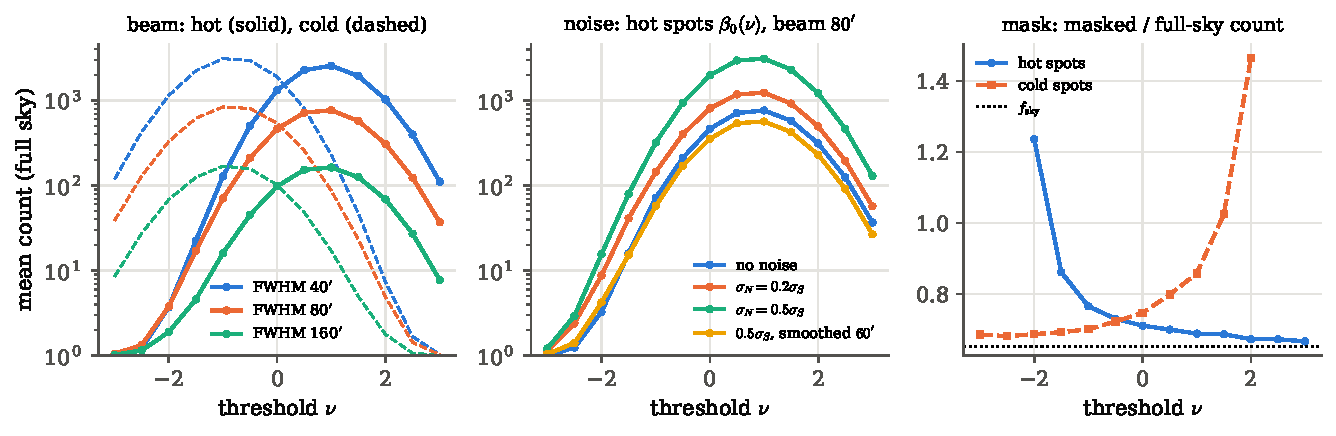
\includegraphics[width=\linewidth]{figures/ch12/c_sphere_ops.pdf}
\caption{Three operators on the full-sky Betti curves, $100$ skies each. Left: beams of $40'$, $80'$ and $160'$; the counts of hot spots
(solid) and cold spots (dashed) fall with the beam as $\lambda$ does. Middle: white pixel noise of $0.2$ and $0.5$ times the signal rms on
the $80'$ map multiplies the hot spots; smoothing the noisy map by another $60'$ removes them again. Right: the counts on a masked sky
divided by the full-sky counts, against the observed sky fraction (dotted).}
\label{12c:fig:sphere-ops}
\end{figure}

\paragraph{Noise creates short-lived features.} White noise is added to every pixel of the $80'$ map, with standard deviation
$\sigma_N=0.2$ and $0.5$ times the rms $\sigma_S$ of the beamed signal; the same skies and the same noise draws are used for every level,
so differences between levels are not cosmic variance. Noise has power at every multipole up to the pixel scale, so it raises $\sigma_1$
far more than $\sigma_0$, and with it $\lambda$. The number of finite hot-spot pairs per sky goes from $\CpNfeatZero$ without noise to
$\CpNfeatTwenty$ and $\CpNfeatFifty$, and the hot spots above $\nu=1$ from $\CpHotOneZero$ to $\CpHotOneFifty$ at $\sigma_N=0.5\sigma_S$. Where do
the new features sit in the diagram? \Cref{12c:fig:sphere-noise} shows it: along the diagonal. The stability theorem of
\cref{12b:sec:stability} says that a perturbation of size $\eta$ can only create pairs of persistence at most $2\eta$, and a single pixel
of noise moves the map only locally; the extra features are tiny bumps on the slopes of real hot spots, born and dead within a fraction
of $\sigma$. The number of pairs with persistence below $0.1\sigma$ triples, from $\CpShortZero$ to $\CpShortTwenty$ and $\CpShortFifty$. Smoothing
the noisy map by a further $60'$ is a second operator that undoes most of the first: $\CpNfeatFiftyS$ pairs, $\CpShortFiftyS$ short ones and
$\CpHotOneFiftyS$ hot spots above $\nu=1$, now fewer than without noise because the total beam is wider.

\begin{figure}[htbp]
\centering
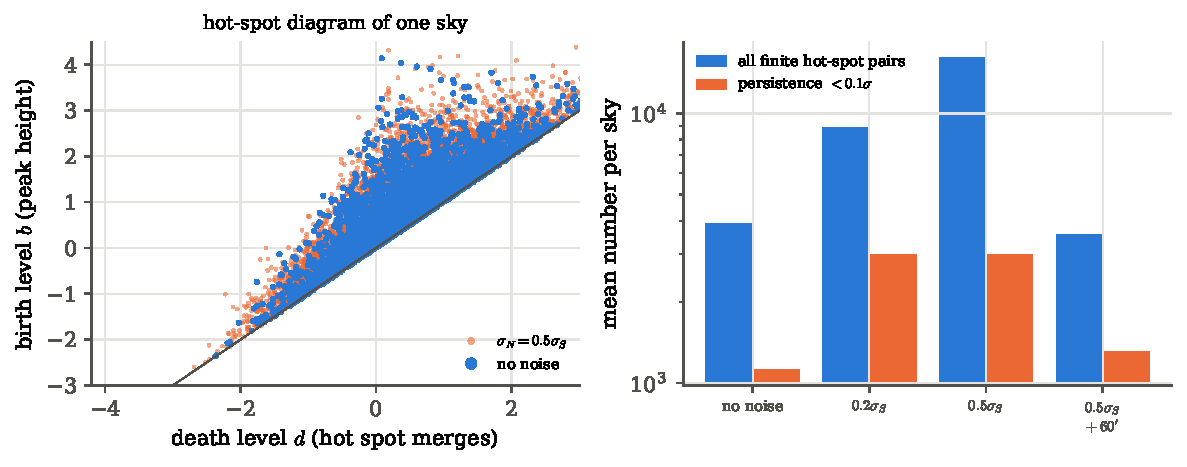
\includegraphics[width=\linewidth]{figures/ch12/c_sphere_noise.pdf}
\caption{Left: the hot-spot persistence diagram of one sky with the $80'$ beam, without noise (blue) and with white noise of $0.5\sigma_S$
(orange); every point is a hot spot born at height $b$ that merges at level $d$. The noisy sky has about four times as many points,
and the extra ones lie close to the diagonal (partly hidden under the blue points, which are drawn on top). Right: the mean number per sky of all finite pairs and of pairs with persistence below $0.1\sigma$, for no noise, $0.2\sigma_S$,
$0.5\sigma_S$, and $0.5\sigma_S$ smoothed by a further $60'$.}
\label{12c:fig:sphere-noise}
\end{figure}

\paragraph{The mask cuts and isolates.} The mask removes the band $|b|<20^\circ$ around the Galactic equator and $100$ discs of radius
$1^\circ$ at random positions, leaving $\fsky=\CpFsky$ of the sky. If the mask simply removed area, every count would fall to $\fsky$ of its
full-sky value. At $\nu=1.5$ the hot spots fall to $\CpMaskRatio$ of the full-sky count: slightly more than $\fsky$, because an island that
crosses the edge of the mask is cut, and a cut island can fall apart into two. Where the excursion set is large, the effect is much bigger
(\cref{12c:fig:sphere-ops}, right). At high thresholds the cold set is almost the whole sky, a single piece on the full sphere; on the
masked sky the band alone splits it into a northern and a southern piece, and every source hole surrounded by hot pixels can isolate
another. The ratio of cold counts climbs far above one. A mask has a topology of its own, two caps with a hundred holes, and it adds that
topology to every large excursion set, the topological counterpart of the mode coupling of \cref{8b:sec:coupling}.

\subsection{A \textit{Planck}-style Gaussianity test on masked, noisy skies}
\label{12c:sec:planck-test}

\paragraph{Their question.} \textit{Planck} asked whether the shapes of the observed microwave sky are those of a Gaussian, isotropic field
\cite{Planck2018VII}. The test (\cref{T3a:sec:planck-mf}) compares the Minkowski functionals of the data with $999$ end-to-end
simulations through a $\chi^2$ and reports the fraction of simulations with a larger $\chi^2$. On the real sky the answer was ``yes, Gaussian'',
with probabilities between $24\%$ and $99.8\%$ for temperature (their Table~5). We reproduce the test, on simulations only (the real sky is
analysed in \cref{ch:13}), with Betti curves in place of the functionals, and with a non-Gaussian sky to see what a failure would look like.

\paragraph{Their equations, in ours.} Their data vector is $36$ numbers, three functionals at twelve thresholds; ours is $p=\CpP$ numbers, hot
and cold counts at thirteen thresholds, after dropping entries that never vary. Their $\chi^2$ (their eqs.~20--22) is \eqref{12c:eq:chi2} with
mean and covariance from simulations; their probability is the simulated $p$-value \eqref{12c:eq:psim}, whose validity we derived in
\eqref{12c:eq:psim-valid}. Their genus is \eqref{12c:eq:chi-hotcold} divided by the sky area. Nothing else is needed.

\paragraph{Our setup.} The null model is a Gaussian sky with the $80'$ beam, white noise of $0.2\sigma_S$ and the mask above: $\CpNnull$
skies, of which $\CpNcov$ give the mean and the covariance (Hartlap factor $\CpHart$) and $\CpNref$ the reference distribution of $\chi^2$.
Calibration: we split the reference skies in two, use one half as the reference and test the other $\CpCalibN$ Gaussian skies
against it; $\CpCalib\%$ of them get $p<0.05$, with an uncertainty of about $\CpCalibSd\%$, and a two-sample
Kolmogorov--Smirnov test of the two halves gives $p=\CpCalibKS$: with only $\CpCalibN$ test skies, both are consistent
with a calibrated test. (Ranking each reference sky among all the others would give
$5\%$ whatever the skies, since the ranks of a set among itself are just a reordering.) The alternative
skies are made as in \cref{12c:sec:model}, now on the sphere: before the beam, the Gaussian sky $s$ becomes $s+a(s^2-\sigma^2)/\sigma$, and each
multipole is rescaled by $R_\ell=\sqrt{C_\ell^{s}/C_\ell^{\phi}}$ so that the power spectrum is unchanged; $R_\ell$ is measured from the
spectra of $\CpNrenorm$ skies with and without the quadratic term, built from the same Gaussian skies so that their ratio is nearly free of
cosmic variance. For each of $a=0.02$, $0.05$ and $0.15$, $\CpNdata$ skies go through the same beam, noise and mask. As a control, the same
test is run with the pseudo-$C_\ell$ of the masked map in a dozen logarithmic bins (\cref{8b:sec:pseudo}).

How large are these amplitudes? On large scales the temperature is $-\Phi/3$, and the local model gives $a=-3f_{\rm NL}\sigma_t$ with
$\sigma_t\approx2\times10^{-5}$ (\cref{T3a:sec:ng-code}). Then $a=0.02$ corresponds to $|f_{\rm NL}|\approx0.02/(6\times10^{-5})\approx330$,
some sixty times the \textit{Planck} error \eqref{T3a:eq:fnl}. Our skies are an exaggerated, pointwise version of the local model at
$N_{\rm side}=128$; they test the machinery, not the inflationary bound.

\paragraph{Side by side.} \Cref{12c:fig:sphere-test} is our version of the bracket plots: the counts of one sky, minus the simulation mean,
in units of the simulation scatter. The Gaussian ``data'' sky stays inside the band at every threshold and has $p=\CpPdataG$. The
non-Gaussian sky with $a=0.15$ leaves it in a characteristic pattern, too many hot spots at high thresholds and too few cold spots below $-1$,
and its $p$ is $\CpPdataNG$, the smallest value $400$ reference skies allow ($1/401$).

\begin{figure}[htbp]
\centering
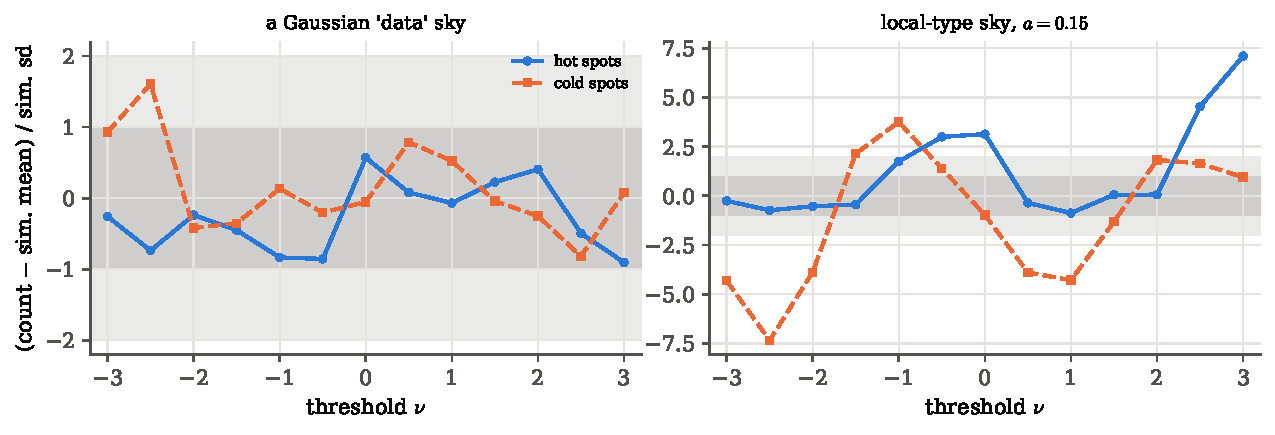
\includegraphics[width=0.9\linewidth]{figures/ch12/c_sphere_test.pdf}
\caption{Hot-spot (solid) and cold-spot (dashed) counts of one masked, noisy, beamed sky, minus the mean of $600$ Gaussian simulations
processed identically, in units of their standard deviation; grey bands: $\pm1$ and $\pm2$. Left: a Gaussian sky, bracketed by the
simulations as \textit{Planck}'s sky was. Right: a local-type sky with $a=0.15$ and the same power spectrum: many thresholds are several
standard deviations out.}
\label{12c:fig:sphere-test}
\end{figure}

\begin{center}
\small
\begin{tabularx}{\linewidth}{@{}>{\raggedright\arraybackslash}p{2.6cm}>{\raggedright\arraybackslash}X>{\raggedright\arraybackslash}X@{}}
\toprule
 & \textit{Planck} 2018 \cite{Planck2018VII} & ours\\
\midrule
summary & $v_0,v_1,v_2$ at $12$ thresholds ($36$) & hot, cold counts at $13$ thresholds ($\CpP$)\\
simulations & $999$ FFP10, full pipeline & $\CpNcov+\CpNref$ Gaussian, beam $+$ white noise $+$ mask\\
resolution & $N_{\rm side}$ $16$ to $2048$ & $N_{\rm side}=\CpNside$, $80'$\\
sky fraction & $\approx0.75$ & $\CpFsky$\\
Gaussian sky, probability & $24\%$ to $99.8\%$ (real $T$ maps) & $p=\CpPdataG$ (one Gaussian sky); $\CpCalib\pm\CpCalibSd\%$ below $0.05$\\
non-Gaussian sky & not seen & $a=0.02$: median $p=\CpMedTwo$, $\CpPowTwo\%$ detected\\
 & & $a=0.05$: median $p=\CpMedFive$, $\CpPowFive\%$ detected\\
 & & $a=0.15$: median $p=\CpMedFifteen$, $\CpPowFifteen\%$ detected\\
same, pseudo-$C_\ell$ & --- & $\CpPclPowTwo\%$, $\CpPclPowFive\%$, $\CpPclPowFifteen\%$ detected\\
\bottomrule
\end{tabularx}
\end{center}

\paragraph{Why they differ, and what the control shows.} The numbers in the two columns answer different questions, and the differences
have stated causes. \textit{Planck}'s probabilities are for the real sky, so they say the sky is Gaussian; ours are for skies whose answer we
know, so they say whether the test works: Gaussian skies are flagged at $\CpCalib\pm\CpCalibSd\%$, to be compared with the nominal
$5\%$, and non-Gaussian ones are caught with a power that rises
from $\CpPowTwo\%$ at $a=0.02$ to $\CpPowFive\%$ at $a=0.05$. \textit{Planck}'s simulations contain the real noise, its anisotropy across the sky,
the component-separation residuals and lensing; ours contain white noise only, so our null distribution is narrower than theirs would be,
and our power is an upper bound for a sky with real systematics. The pseudo-$C_\ell$ control behaves as designed: its median $p$ stays near
the middle ($\CpPclMedTwo$, $\CpPclMedFive$, $\CpPclMedFifteen$) and its detection rate near the false-alarm rate, except at $a=0.15$, where it
rises to $\CpPclPowFifteen\%$. The spectra have the same mean, to within $\CpPclPullMax$ standard errors of a $100$-sky average in the worst bin;
what differs is their scatter: the quadratic term adds a connected four-point function, which inflates the variance of each $\hat C_\ell$ (the
pitfall of \cref{12c:sec:model}), and an omnibus $\chi^2$ notices a larger scatter as well as a shifted mean.

\paragraph{Lesson.} Rebuilding the test showed what its probabilities rest on: the null hypothesis enters only through simulations processed
exactly like the data, so the mask, the beam and the noise need no formula, and the test is only as good as those simulations.
\section{When there is no likelihood: inference from the simulator alone}
\label{12c:sec:abc}

Every inference so far went through a formula for $P(\bm S\given\epsilon)$: Gaussian, with a mean and a covariance read off
simulations. \Cref{12c:sec:coverage} showed what that formula costs: a covariance frozen at one value of $\epsilon$ made the
intervals several per cent too narrow, and counts of rare features are not Gaussian anyway. Yet the simulator itself never assumed
anything Gaussian about the counts. For any $\epsilon$ it produces maps, and the counts of those maps \emph{are} draws from the true
$P(\bm S\given\epsilon)$. The likelihood is defined implicitly by the simulator, even if we cannot write it down. Can we get a
posterior using only the ability to simulate?

\paragraph{The question.} Without writing $P(\bm S\given\epsilon)$, which values of $\epsilon$ could have produced the map we observed,
and how probable is each, using nothing but the prior and the simulator?

\subsection{Rejection ABC}
\label{12c:sec:rejection}

The plainest answer is a direct imitation of Bayes' theorem by sampling, \newterm{approximate Bayesian computation} (ABC). Repeat
many times: draw $\epsilon$ from the prior; simulate a map with that $\epsilon$; compute its summary $t$; keep $\epsilon$ if $t$ lands
within a distance $\delta$ of the observed $t_{\rm obs}$. The kept values are draws from the posterior. Why? A value $\epsilon$ is
proposed with probability density $p(\epsilon)$ and, once proposed, kept with probability $\Prob(|t-t_{\rm obs}|<\delta\given\epsilon)$.
So the density of kept values is
\begin{align}
  p_{\rm kept}(\epsilon)
  &\eqby{1}\frac{p(\epsilon)\,\Prob(|t-t_{\rm obs}|<\delta\given\epsilon)}{\int p(\epsilon')\,\Prob(|t-t_{\rm obs}|<\delta\given\epsilon')\,\dd\epsilon'}
   \eqby{2}\frac{p(\epsilon)\,\int_{t_{\rm obs}-\delta}^{t_{\rm obs}+\delta}p(t\given\epsilon)\,\dd t}
               {\int p(\epsilon')\int_{t_{\rm obs}-\delta}^{t_{\rm obs}+\delta}p(t\given\epsilon')\,\dd t\,\dd\epsilon'}\nonumber\\
  &\relby{3}{\approx}\frac{p(\epsilon)\,2\delta\,p(t_{\rm obs}\given\epsilon)}{\int p(\epsilon')\,2\delta\,p(t_{\rm obs}\given\epsilon')\,\dd\epsilon'}
   \eqby{4}p(\epsilon\given t_{\rm obs}) .
  \label{12c:eq:abc}
\end{align}
\begin{explain}
  \item The probability of ``proposed at $\epsilon$ and kept'', normalised over everything kept (Bayes' theorem with the event
        ``kept'').
  \item The probability of landing in the window is the integral of the density of $t$ over the window.
  \item For a small window the density is nearly constant across it: the integral is its width times the value at the centre.
  \item The $2\delta$ cancels, and what remains is Bayes' theorem for the posterior given $t_{\rm obs}$.
\end{explain}
No likelihood was evaluated. The simulator decided, by producing or not producing a $t$ close to $t_{\rm obs}$, how readily each
$\epsilon$ could have produced the observation; this is the likelihood of \cref{ch:05}, estimated by counting. The approximation
is the finite window: as $\delta\to0$ the answer becomes exact, and the fraction of kept simulations goes to zero.

\begin{figure}[htbp]
\centering
\begin{tikzpicture}[
  bx/.style={draw=black!45,rounded corners=2pt,align=center,font=\small,text width=2.7cm,minimum height=1.0cm,fill=formblue!6},
  arr/.style={->,thick,black!55}]
  \node[bx] (pr) at (0,0) {draw $\epsilon$\\ \scriptsize from the prior};
  \node[bx] (sim) at (3.6,0) {simulate a map\\ \scriptsize same pipeline as data};
  \node[bx] (sum) at (7.2,0) {summarise\\ \scriptsize $t=\bm w\T(\bm S-\bm\mu_0)$};
  \node[bx,fill=bdryred!6,draw=bdryred!60] (cmp) at (7.2,-2.0) {$|t-t_{\rm obs}|<\delta$?};
  \node[bx,fill=tangentgreen!8,draw=tangentgreen!70] (keep) at (3.6,-2.0) {keep $\epsilon$\\ \scriptsize posterior draw};
  \node[bx,fill=black!3] (obs) at (10.4,-2.0) {observed map\\ \scriptsize $t_{\rm obs}$};
  \draw[arr] (pr) -- (sim);
  \draw[arr] (sim) -- (sum);
  \draw[arr] (sum) -- (cmp);
  \draw[arr] (obs) -- (cmp);
  \draw[arr] (cmp) -- node[above,font=\scriptsize]{yes} (keep);
  \draw[arr] (cmp.south) -- ++(0,-0.55) -| node[pos=0.25,below,font=\scriptsize]{no: discard, repeat} (pr.south);
\end{tikzpicture}
\caption{Rejection ABC. Parameters are drawn from the prior and pushed through the simulator; only those whose simulated summary
lands close to the observed one survive. Surviving in proportion to how often each $\epsilon$ produces something like the data
is exactly the likelihood weighting of Bayes' theorem.}
\label{12c:fig:abcloop}
\end{figure}

\subsection{Why compress first}
\label{12c:sec:compress}

The window in \eqref{12c:eq:abc} is around one number. Why not around the whole $26$-number Betti vector? Because in many
dimensions ``close'' almost never happens. Measure the distance between a simulated vector and the observed one in units of the
noise, $D^2=(\bm S-\bm S_{\rm obs})\T\Cmat^{-1}(\bm S-\bm S_{\rm obs})$. Even a simulation with exactly the right $\epsilon$ differs from
the observation by two independent fluctuations, so its $\bm S-\bm S_{\rm obs}$ has covariance $2\Cmat$ and
\begin{equation}
  \E[D^2]=\Tr\bigl(\Cmat^{-1}\,2\Cmat\bigr)=2p=52,\qquad D\approx7 ,
  \label{12c:eq:curse}
\end{equation}
while the effect of a wrong $\epsilon$ adds only $(\Delta\epsilon)^2F$ to $D^2$. In $26$ dimensions every simulation is far away, the
right $\epsilon$ and the wrong one almost equally; keeping the nearest few per cent selects mostly on noise. This is the curse of
dimensionality, and the cure is to compress the data to as few numbers as there are parameters while keeping the information.

\paragraph{The score as a compression.} If the mean were linear, $\bm\mu(\epsilon)=\bm\mu_0+\epsilon\bm d$, the Gaussian log-likelihood
would be
\begin{align}
  \ln\Like(\epsilon)
  &\eqby{1}-\tfrac12(\bm S-\bm\mu_0-\epsilon\bm d)\T\Cmat^{-1}(\bm S-\bm\mu_0-\epsilon\bm d)\nonumber\\
  &\eqby{2}-\tfrac12(\bm S-\bm\mu_0)\T\Cmat^{-1}(\bm S-\bm\mu_0)+\epsilon\,\bm d\T\Cmat^{-1}(\bm S-\bm\mu_0)-\tfrac12\epsilon^2F ,
  \label{12c:eq:sufficient}
\end{align}
\begin{explain}
  \item \eqref{12c:eq:like} with the linear mean.
  \item Multiply out; the two cross terms are equal because $\Cmat^{-1}$ is symmetric; $F=\bm d\T\Cmat^{-1}\bm d$.
\end{explain}
The first term does not depend on $\epsilon$ and cancels in any posterior. The data enter the $\epsilon$-dependence only through
$\bm d\T\Cmat^{-1}(\bm S-\bm\mu_0)$, the score \eqref{12c:eq:score}. Two maps with the same score have the same posterior: the score
is a sufficient statistic for this model (\cref{3b:sec:recipe-suff}), and dividing it by $F$ turns it into an estimate of $\epsilon$,
\begin{equation}
  t=\frac{\bm d\T\Cmat^{-1}(\bm S-\bm\mu_0)}{\bm d\T\Cmat^{-1}\bm d} .
  \label{12c:eq:tcomp}
\end{equation}
For a model that is only approximately linear and Gaussian, $t$ is no longer exactly sufficient, but it keeps nearly all the Fisher
information about $\epsilon$ near the fiducial point. This approximate score compression is how simulation-based analyses in cosmology
reduce long data vectors to one number per parameter \cite{Alsing2019}. Note what the Gaussian model is used for here: only to choose
the weights $\bm w=\Cmat^{-1}\bm d/F$. If the weights are imperfect we lose some information, but the posterior is still correct for the
$t$ we use, because ABC takes the distribution of $t$ from the simulator.

\subsection{ABC on one map}
\label{12c:sec:abc-run}

The script \pyname{code/ch12/c07_abc.py} applies this to the same mock map as \cref{12c:sec:onemap} (seed $\CfMock$,
$\epsilon_{\rm true}=0.05$). It draws $\CbN$ new maps with $\epsilon$ uniform on $(-0.15,0.15)$:
\pyfile[firstline=44,lastline=47]{code/ch12/c07_abc.py}{One ABC simulation: prior draw, map, summary}
\noindent and then keeps the $\CbKeepPct\%$ whose compressed summary is nearest to the observed one:
\pyfile[firstline=76,lastline=90]{code/ch12/c07_abc.py}{Compression weights, the observed summary, and rejection on $t$ and on all $26$ numbers}
\noindent Line by line: the weights \pyname{w} are $\Cmat^{-1}\bm d/F$ from the null maps and the derivative of \cref{12c:sec:deriv};
\pyname{t_obs} is the observed map's compressed summary, $\CbTobs$; the $\CbKeep$ simulations with $t$ nearest to it are kept, which sets
the window at $\delta=\CbTol$; for comparison the $\CbKeep$ simulations nearest in the full $26$-dimensional distance $D$ are kept as
well.

\begin{figure}[htbp]
\centering
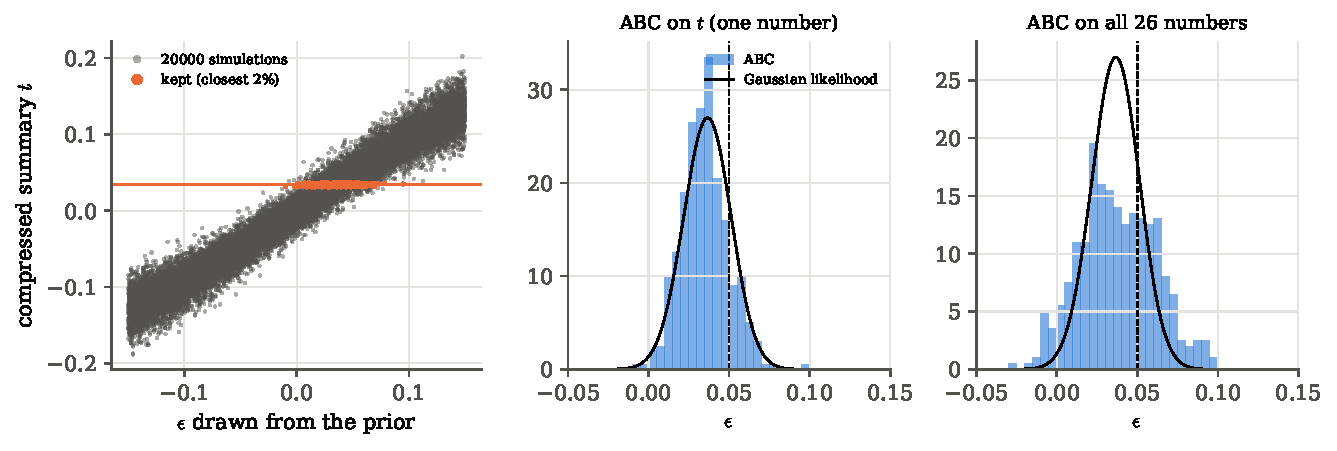
\includegraphics[width=\linewidth]{figures/ch12/c_abc.pdf}
\caption{Left: the compressed summary $t$ of $20000$ maps against the $\epsilon$ they were made with. The band is the likelihood seen
sideways: at each $\epsilon$, the spread of $t$ is its sampling distribution. The horizontal line is the observed $t$; the orange points,
the simulations nearest to it, are the ABC posterior draws. Middle: their histogram against the Gaussian-likelihood posterior of
\cref{12c:sec:onemap}. Right: the same with the window around all $26$ numbers: much broader.}
\label{12c:fig:abc}
\end{figure}

\paragraph{The result.} ABC on $t$ gives $\epsilon=\CbMeanT\pm\CbSdT$. ABC on all $26$ numbers gives $\CbMeanAll\pm\CbSdAll$, and its
kept simulations are at distances up to $D=\CbDistTol$, not far below the $D\approx7$ that \eqref{12c:eq:curse} predicts even for the right
$\epsilon$: the selection is mostly noise, as expected. The Gaussian likelihood gave $\CbMeanL\pm\CbSdL$.

\paragraph{Is ABC more honest?} On this one map ABC on $t$ comes out a little narrower than the Gaussian likelihood ($\CbSdT$
against $\CbSdL$). One map cannot settle the question. The width that $\CbKeep$ kept simulations give is itself uncertain by a few per
cent, and the width of either posterior changes from map to map. But the ABC simulations do not depend on which map was observed, so the
same $\CbN$ of them serve all $\CbNmaps$ mock maps of \cref{12c:sec:coverage}, at no extra cost. Over those maps the typical (median) ABC
width is $\CbSdMed$, against $\CfSdMedFive$ for the Gaussian likelihood. The ABC interval contains the true $\epsilon$ in
$\CbCover\pm\CbCoverErr\%$ of the maps; the Gaussian interval does so in $\CfCoverFive\%$, and both should do so in $68\%$.

Where does the extra width come from? The left panel of \cref{12c:fig:abc} shows it. A straight-line fit of $t$ against $\epsilon$ has
slope $\CbSlope$ (an exactly linear model would give $1$), and the points scatter around the line by $\CbScatter$. The scatter grows with
$\epsilon$, from $\CbScZero$ near $\epsilon=0$ to $\CbScFive$ near $0.05$. A posterior from $t$ alone is about as wide as the scatter
divided by the slope, $\CbScFive/\CbSlope\approx0.016$ near the truth. The window adds little: $\delta=\CbTol$ adds $\delta^2/3$ to the
variance, about one per cent. The Gaussian likelihood instead assumed the $\epsilon=0$ scatter everywhere, which gives $\CbSigF$. ABC
uses the scatter the simulator really produces at each $\epsilon$, so its intervals are wider and contain the truth about as often as they
should. That is the width the coverage test asked for.

\paragraph{What it cost.} ABC used $\CbN$ simulations to give one posterior, against about $5000$ for the Gaussian-likelihood analysis,
which then serves any number of maps. Rejection wastes $98\%$ of its simulations, and shrinking $\delta$ wastes more. Modern
simulation-based inference keeps every simulation: it fits a flexible model of the density $p(t\given\epsilon)$ or $p(\epsilon\given t)$
(a neural density estimator) to the simulated pairs, and chooses where to simulate next by where the posterior is
\cite{Alsing2019}. Akeret et al.\ built the same rejection-and-refinement loop for cosmological forward models \cite{Akeret2015}. The logic
is \eqref{12c:eq:abc} in every case: the simulator defines the likelihood, and the data are compared with it through a few
well-chosen numbers.

\begin{keyidea}[The simulator is the likelihood]
If we can simulate the data for any parameter value, we never need to write $P(\bm S\given\theta)$: keeping parameter draws whose
simulations resemble the data samples the posterior \eqref{12c:eq:abc}. ``Resemble'' must be measured on a few informative numbers,
such as the score-compressed summary \eqref{12c:eq:tcomp}, because in many dimensions nothing resembles anything.
\end{keyidea}
\section{Reproducing the literature: topology and $f_{\rm NL}$}
\label{12c:sec:repro}

Two papers made the claim tested above, that topological summaries see primordial non-Gaussianity that the power
spectrum does not, and turned it into numbers. Cole and Shiu forecast $f_{\rm NL}$ from persistence diagrams of CMB maps
\cite{ColeShiu2018}; Biagetti, Cole and Shiu detected it in the topology of simulated dark-matter haloes \cite{Biagetti2021}. A third,
Heydenreich and collaborators, did the same for cosmological parameters from weak-lensing mass maps \cite{Heydenreich2021}, and was
reproduced in \cref{12w:sec:beyond}. We redo the key result of each of the first two on our maps, with the machinery of the previous
sections, and see what survives the change of setting.

\subsection{Cole and Shiu (2018): are persistence diagrams worth more than Betti curves?}
\label{12c:sec:repro-cs}

\paragraph{Their question.} Betti curves count the features alive at each threshold; a persistence diagram also records which birth goes with
which death. The diagram therefore contains the Betti curves (\eqref{12b:eq:betti-curve}) and possibly more. Is the extra information about
local non-Gaussianity worth having? In 2017 nobody had tried persistence diagrams on the CMB.

\paragraph{Their setup.} They used public simulations of CMB temperature with local non-Gaussianity: for each of $1000$ realisations, a
Gaussian set of $a_{\ell m}$ and a separate non-Gaussian part, combined as $a_{\ell m}=a^{\rm G}_{\ell m}+f_{\rm NL}a^{\rm NG}_{\ell m}$ so that any
$f_{\rm NL}$ can be dialled in. From each sky they cut two square patches of $1024\times1024$ pixels around the poles, and computed the persistence
diagrams of the sublevel filtration (lowering the threshold from the coldest pixel up) and the Betti curves. The diagrams were binned into
two-dimensional histograms (birth $\times$ persistence), and the Betti curves divided by their maximum.

\begin{center}
\small
\begin{tabular}{ll}
\toprule
resolution & $N_{\rm side}=512$, $\ell_{\max}=1024$, Gaussian smoothing $\theta_s=90'$ (FWHM $212'$)\\
maps & $2000$ patches of $1024^2$ pixels per value of $f_{\rm NL}\in\{0,10,25,50,100\}$\\
mean $\bm\mu(f_{\rm NL})$ & average of $800$ patches at $f_{\rm NL}=0,10,50$\\
covariance & $2000$ patches at $f_{\rm NL}=0$, with the Hartlap factor\\
statistics & $\beta_0$, $\beta_1$, $\beta_0+\beta_1$; histograms PD0, PD1, PD0+PD1\\
\bottomrule
\end{tabular}
\end{center}

\paragraph{Their key equation.} Their likelihood (their eq.~4.2) is our \eqref{12c:eq:like}, $\ln\Like(f_{\rm NL})=-\frac12(\bm d-\bm\mu(f_{\rm NL}))\T
\Cmat^{-1}(\bm d-\bm\mu(f_{\rm NL}))$, evaluated for ``data'' $\bm d$ equal to the simulated mean at $f_{\rm NL}=0$, and fitted with a Gaussian in
$f_{\rm NL}$ whose width is the quoted error. With noise-free data at the fiducial point and a mean that is linear in the parameter,
$\bm\mu(f)=\bm\mu_0+f\bm\mu'$,
\begin{align}
  \ln\Like(f)
  &\eqby{1}-\tfrac12(\bm\mu_0-\bm\mu_0-f\bm\mu')\T\Cmat^{-1}(\bm\mu_0-\bm\mu_0-f\bm\mu')
   \eqby{2}-\tfrac12f^2\,\bm\mu'^{\mathsf T}\Cmat^{-1}\bm\mu'\nonumber\\
  &\eqby{3}-\frac{f^2}{2\sigma^2},\qquad \sigma=\bigl(\bm\mu'^{\mathsf T}\Cmat^{-1}\bm\mu'\bigr)^{-1/2} ,
  \label{12c:eq:cs-like}
\end{align}
\begin{explain}
  \item Insert $\bm d=\bm\mu_0$ and the linear mean.
  \item The constant vectors cancel; $f$ comes out of both factors.
  \item A Gaussian in $f$ centred on zero, with variance the inverse of the quadratic coefficient.
\end{explain}
The fitted width is the Fisher error \eqref{12c:eq:fisher}. Symbol map: their $f_{\rm NL}$ is our $\epsilon$ up to a constant factor (the
variance of their potential against our unit-variance $g$), so absolute errors cannot be compared, but \emph{ratios} of errors between
statistics can. We compare every error with that of $\beta_0+\beta_1$.

\paragraph{What we compute.} \pyname{code/ch12/c08_repro.py} evaluates \eqref{12c:eq:fisher} for the same six statistics on our $256^2$ maps,
with derivatives from shared seeds at $\epsilon=\pm0.05$ and the covariance from the $1000$ null maps:
\pyfile[firstline=33,lastline=51]{code/ch12/c08_repro.py}{Fisher error for one statistic (optionally with each curve divided by its maximum)}
\noindent It also repeats the Betti rows with every curve divided by its own maximum, as they did.

\paragraph{Side by side.}
\begin{center}
\small
\begin{tabular}{lcccc}
\toprule
statistic & Cole \& Shiu $\Delta f_{\rm NL}$ & ratio & ours $\sigma(\epsilon)$ & ratio\\
\midrule
$\beta_0$ & $67.4$ & $\CrThBZero$ & $\CrBZero$ & $\CrRelBZero$\\
$\beta_1$ & $66.1$ & $\CrThBOne$ & $\CrBOne$ & $\CrRelBOne$\\
$\beta_0+\beta_1$ & $60.6$ & $\CrThBBoth$ & $\CrBBoth$ & $\CrRelBBoth$\\
PD0 & $39.1$ & $\CrThPZero$ & $\CrPZero$ & $\CrRelPZero$\\
PD1 & $37.4$ & $\CrThPOne$ & $\CrPOne$ & $\CrRelPOne$\\
PD0$+$PD1 & $35.8$ & $\CrThPBoth$ & $\CrPBoth$ & $\CrRelPBoth$\\
\bottomrule
\end{tabular}
\end{center}

\begin{figure}[htbp]
\centering
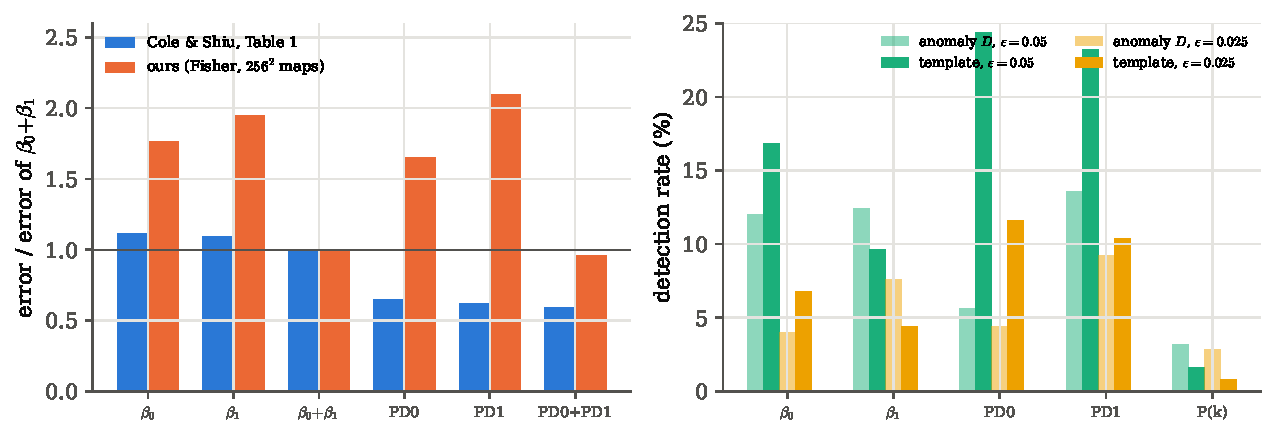
\includegraphics[width=\linewidth]{figures/ch12/c_repro.pdf}
\caption{Left: errors on the non-Gaussianity amplitude relative to that of $\beta_0+\beta_1$, from Cole and Shiu's Table~1 (blue) and from our
Fisher matrices (orange). They find the diagrams $40\%$ better than the curves; on our maps the two are equal, while each curve alone is about
twice as bad as the pair. Right: detection rates of $\epsilon=0.05$ and $0.025$ with Biagetti et al.'s anomaly distance (pale) and template
statistic (dark), for four topological summaries and the power spectrum.}
\label{12c:fig:repro}
\end{figure}

\paragraph{Why they differ.} Two results disagree. Their diagrams beat their Betti curves by a factor $0.59$; ours tie. And their $\beta_0$ and
$\beta_1$ each nearly match the pair, while ours are each about twice as bad. Go through the differences in setup one at a time.

\emph{The normalisation of the Betti curves.} Dividing each curve by its maximum throws away its overall amplitude. On our maps it costs
something: $\beta_0+\beta_1$ normalised gives $\CrNormBBoth$ instead of $\CrBBoth$, so that the diagrams measured against normalised curves would come out at
$\CrPBoth/\CrNormBBoth\approx\CrPdOverNorm$ instead of $1$. Part of their gap, not all of it.

\emph{Where the signal lives.} In our model the quadratic term is applied to the field we observe, smoothed once; most of what $\epsilon$ does is
move pixel values, a one-point effect (\cref{12c:sec:shift}), and it shows up as more pieces in the hot tail and fewer lakes in the cold tail,
two nearly independent witnesses (\cref{12c:sec:power}). Betti curves sampled out to $\pm3\sigma$ capture that completely, and $\beta_0$ and
$\beta_1$ see different tails, so each alone loses half. In their CMB maps the quadratic term acts on the primordial potential and passes
through the acoustic transfer function, which mixes neighbouring points (\cref{T3a:sec:ng-code}); less of the signal is a simple shift of values,
and more of it is in how features are arranged. If that is the reason, removing the one-point part from our maps should restore their
result. It does: at area-fraction thresholds, where the one-point effect is gone by construction, our persistence histograms give
$\sigma(\epsilon)=\CfSigPdA$ against $\CfSigBettiA$ for the Betti curves, a ratio of $\CfSigPdA/\CfSigBettiA\approx\CfPdAOverBettiA$, against
their $0.59$. We cannot prove from their paper
that this is the whole explanation, but it is the one we can test, and it passes.

\emph{Smaller differences.} Their histograms are finer than our $10\times5$ bins; their patches have edges, which add pieces along the boundary
(the reason they normalised); their maps hold far more correlation areas than our $256^2$ pixels. None of these changes the ratios we compare
by as much as the two effects above.

\paragraph{Lesson.} ``Persistence diagrams carry more information than Betti curves'' is not a theorem; it depends on where in the field the signal
lives. When the signal is a shift of values, a good Betti curve already has it; when it is in the arrangement, birth--death pairs add
information, and on our maps they add it in the same proportion as on Cole and Shiu's.

\subsection{Biagetti, Cole and Shiu (2021): detecting $f_{\rm NL}$ without a likelihood}
\label{12c:sec:repro-bcs}

\paragraph{Their question.} Can the topology of the dark-matter halo distribution reveal a local $f_{\rm NL}$ as small as $10$, through the
structures it affects at scales of about $10\,h^{-1}$Mpc, where the usual signature in the halo power spectrum (a bias that grows on large scales)
is negligible? And how can one attach a significance to such a detection without writing a likelihood for persistence summaries?

\paragraph{Their setup.} $N$-body simulations with Gaussian initial conditions (``G85L'') and with $f_{\rm NL}=10$ (``NG10L''), in boxes whose five
realisations add up to $40\,(h^{-1}{\rm Gpc})^3$, about a Euclid-like volume; persistence diagrams of the halo catalogues with a distance-to-measure
filtration; summaries built from the diagrams (distributions of births $B_p$, deaths $D_p$, persistences, and Betti curves). Significance comes
from splitting the realisations into a ``survey'' and a ``fiducial'' set in all possible ways: Gaussian against Gaussian splits give the null
distribution, Gaussian against non-Gaussian splits give the detection rate. Two statistics are used.

\paragraph{Their equations, derived.} The \emph{anomaly} distance (their eq.~4.1) is
\begin{equation}
  D_{\rm anomaly}=\Bigl[\frac1N\sum_{i=1}^N\frac{(d_i-\mu_i)^2}{\sigma_i^2}\Bigr]^{1/2},
  \label{12c:eq:anomaly}
\end{equation}
with $\mu_i$, $\sigma_i$ the mean and standard deviation of entry $i$ under the null: the $\chi^2$ of \eqref{12c:eq:chi2} with the covariance
replaced by its diagonal, divided by $N$, square-rooted. It is an omnibus test, and it ignores correlations. A detection is a $D$ above the
$95$th percentile of the Gaussian splits. The \emph{template} (their eqs.~4.2--4.3) is the mean difference between a strongly non-Gaussian
($f_{\rm NL}=250$) and a Gaussian simulation \emph{with the same initial seed}, $\bm T=\overline{\bm S_{\rm NG}-\bm S_{\rm G}}$, and the statistic is the
projection of the data on it, $D_{\rm template}=(\bm S-\bm\mu)\cdot\bm T/\sigma_T$, with $\sigma_T$ its standard deviation under the null; a detection
is a value above the $97.5$th percentile. What is the template, in our language? To first order the shared-seed difference is
$\bm T\approx f_{\rm big}\,\bm d$, the derivative of \cref{12c:sec:deriv} times the large amplitude, so
\begin{align}
  D_{\rm template}
  &\eqby{1}\frac{f_{\rm big}\,\bm d\T(\bm S-\bm\mu)}{\sqrt{\Var[f_{\rm big}\,\bm d\T(\bm S-\bm\mu)]}}
   \eqby{2}\frac{\bm d\T(\bm S-\bm\mu)}{\sqrt{\bm d\T\Cmat\bm d}} ,
  \label{12c:eq:template}
\end{align}
\begin{explain}
  \item $\bm T\approx f_{\rm big}\bm d$, and $\sigma_T$ is the null standard deviation of the projection.
  \item $f_{\rm big}$ cancels; the variance of $\bm a\T\bm x$ is $\bm a\T\Cmat\bm a$.
\end{explain}
This is the score \eqref{12c:eq:score} with $\Cmat^{-1}$ replaced by the identity: it aims at the right direction but does not weight the entries
by their noise. How much does that cost? For any weights $\bm w$, the statistic $\bm w\T(\bm S-\bm\mu)$ has, at a small $\epsilon$, mean $\epsilon\,\bm w\T\bm d$ and
standard deviation $\sqrt{\bm w\T\Cmat\bm w}$. Write $\bm a=\Cmat^{1/2}\bm w$ and $\bm b=\Cmat^{-1/2}\bm d$; then
\begin{align}
  \frac{\bm w\T\bm d}{\sqrt{\bm w\T\Cmat\bm w}}
  \eqby{1}\frac{\bm a\T\bm b}{|\bm a|}
  \relby{2}{\le}|\bm b|
  \eqby{3}\sqrt{\bm d\T\Cmat^{-1}\bm d}=\sqrt F ,
  \label{12c:eq:cauchy}
\end{align}
\begin{explain}
  \item $\bm w\T\bm d=\bm w\T\Cmat^{1/2}\Cmat^{-1/2}\bm d=\bm a\T\bm b$ and $\bm w\T\Cmat\bm w=|\bm a|^2$.
  \item Cauchy--Schwarz, with equality when $\bm a\propto\bm b$, that is $\bm w\propto\Cmat^{-1}\bm d$: the score.
  \item $|\bm b|^2=\bm d\T\Cmat^{-1}\bm d$.
\end{explain}
The score is the best linear statistic; the template reaches the bound only if $\bm d$ happens to be an eigenvector of $\Cmat$.
\Cref{12c:fig:whiten} shows the geometry.

\begin{figure}[htbp]
\centering
\begin{tikzpicture}[scale=1.25]
  \draw[faint,->] (-2.6,0) -- (2.8,0) node[right,black,font=\small] {entry 1};
  \draw[faint,->] (0,-1.1) -- (0,1.9) node[above,black,font=\small] {entry 2};
  \fill[formblue!10] (0,0) ellipse (2 and 0.5);
  \draw[formblue,thick] (0,0) ellipse (2 and 0.5);
  \node[formblue,font=\small,anchor=north west] at (1.25,-0.45) {null scatter $\Cmat$};
  \draw[->,very thick,bdryred] (0,0) -- (0.9,0.9);
  \node[bdryred,font=\small,anchor=west] at (0.92,0.95) {response $\bm d$ (template)};
  \draw[->,very thick,tangentgreen] (0,0) -- ({1.4/sqrt(257)},{1.4*16/sqrt(257)});
  \node[tangentgreen!70!black,font=\small,anchor=east] at ({1.4/sqrt(257)-0.05},{1.4*16/sqrt(257)}) {score weights $\Cmat^{-1}\bm d$};
\end{tikzpicture}
\caption{Why whitening matters. Two entries of a data vector, the first very noisy (long axis of the null ellipse) and the second quiet. A small
$\epsilon$ moves the mean along $\bm d$ (red), equally in both. Projecting on $\bm d$ mixes in the large noise of entry~1; the score weights
$\Cmat^{-1}\bm d$ (green) lean on the quiet entry. For the ellipse drawn, with standard deviations $2$ and $0.5$, the signal-to-noise per unit
$\epsilon$ is $2/\sqrt{4.25}=0.97$ along $\bm d$ and $\sqrt{4.25}=2.06$ along $\Cmat^{-1}\bm d$.}
\label{12c:fig:whiten}
\end{figure}

\paragraph{What we compute.} The same two statistics on our maps, in \pyname{c08_repro.py}: null mean and standard deviations from the
$1000$ null maps, the null distributions of $D_{\rm anomaly}$ and $D_{\rm template}$ from the $500$ check maps, the template from the shared-seed
differences between $\epsilon=0.1$ and $\epsilon=0$ for grid seeds $0$--$249$ (twice the tested amplitude, where theirs was twenty-five times), and
detection rates for seeds $250$--$499$ at $\epsilon=0.05$ and $0.025$, for $\beta_0$, $\beta_1$, PD0, PD1 and the power spectrum.

\paragraph{Side by side.} Biagetti et al.\ detect $f_{\rm NL}=10$ in about $85\%$ of survey volumes with the template on $B_1$ (births of loops)
and $74\%$ on $D_1$ (deaths of loops), at the $97.5\%$ level, and several summaries reach detection rates above $60\%$ with the anomaly distance
at the $95\%$ level; the halo power spectrum, on large scales, does about as well as the topology. On our maps, at $\epsilon=0.05$:
\begin{center}
\small
\begin{tabular}{lccccc}
\toprule
 & $\beta_0$ & $\beta_1$ & PD0 & PD1 & $P(k)$\\
\midrule
anomaly $D$, $95\%$ (\%) & $\CrAnBZeroFive$ & $\CrAnBOneFive$ & $\CrAnPZeroFive$ & $\CrAnPOneFive$ & $\CrAnPkFive$\\
template, $97.5\%$ (\%) & $\CrTpBZeroFive$ & $\CrTpBOneFive$ & $\CrTpPZeroFive$ & $\CrTpPOneFive$ & $\CrTpPkFive$\\
\bottomrule
\end{tabular}
\end{center}
and at $\epsilon=0.025$ the template rates are $\CrTpBZeroTwo$, $\CrTpBOneTwo$, $\CrTpPZeroTwo$, $\CrTpPOneTwo$ and $\CrTpPkTwo\%$.

\paragraph{Why they differ.} Each rate comes from $250$ maps, so a rate near $15\%$ is uncertain by
$\sqrt{0.15\times0.85/250}\approx2$ percentage points, and both statistics are judged against the same $500$ check maps. Within
that precision the qualitative pattern is theirs: where the two statistics differ by several such errors, the template beats
the anomaly distance, because it aims (\cref{12c:sec:power}); the anomaly distance, an unweighted omnibus statistic, is the
weakest. The power spectrum is where our setting
departs on purpose: our maps have the same spectrum by construction, so it detects nothing beyond the false-alarm rate, while in a halo catalogue
local $f_{\rm NL}$ changes the large-scale bias and the spectrum does respond. The absolute rates differ because the experiments differ in size, one
$256^2$ map against $40\,(h^{-1}{\rm Gpc})^3$ of haloes. The rates are also low compared with what our data can do, and \eqref{12c:eq:cauchy} says
why: the template is unwhitened. For $\beta_0$ alone the Fisher error is $\CrBZero$, so the score at $\epsilon=0.05$ is shifted by
$0.05/\CrBZero\approx\CrShiftBZero$ standard deviations, and a one-sided test at $97.5\%$ (threshold $1.96$) would detect it about half the time; the template
detects $\CrTpBZeroFive\%$. Our $\beta_0$ curve has entries with very different noise, large counts near the median and small, quiet counts in the
tail where the signal is, exactly the situation of \cref{12c:fig:whiten}.

\paragraph{Lesson.} Their two statistics are the omnibus test and an unwhitened score. Reproducing them showed that the step from anomaly to
template, aiming at the expected signal, is what raises the detection rate, and that the next step, weighting by the inverse covariance, is worth
as much again whenever the entries of the summary are not equally noisy.

\paragraph{Heydenreich et al.\ (2021), recalled.} The weak-lensing analogue was reproduced in \cref{12w:sec:beyond}: persistent Betti numbers of
aperture-mass maps, with a simulated covariance and an emulated mean, constrain $S_8$ better than peak counts, by $44\%$ in figure of merit in their
KV450-like setup and $18\%$ in error for a Euclid-like survey \cite{Heydenreich2021}. It is the same pipeline as for $\epsilon$, with a cosmological
parameter in place of $\epsilon$ and a non-Gaussian field produced by gravity rather than by inflation.
\section{How it is done in research}
\label{12c:sec:research}

Every step from the nine-pixel grid to the ABC posterior was a scaled-down version of an analysis that is run on real data. The steps are the same; the size of the
maps, the realism of the simulations, the number of parameters and the care taken at each step are not. \Cref{12c:fig:research}
lays out the pipeline as a real analysis runs it, for a CMB Gaussianity test or an $f_{\rm NL}$ forecast from topology, and for its
large-scale-structure and lensing relatives.

\begin{figure}[htbp]
\centering
\begin{tikzpicture}[
  st/.style={draw=black!45,rounded corners=2pt,align=center,font=\small,text width=3.0cm,minimum height=1.25cm,fill=formblue!6},
  ck/.style={draw=bdryred!60,rounded corners=2pt,align=center,font=\scriptsize,text width=3.0cm,minimum height=0.9cm,fill=bdryred!4},
  arr/.style={->,thick,black!55}]
  \node[st] (d) at (0,0) {1. data products\\ \scriptsize maps, masks, catalogues};
  \node[st] (s) at (3.7,0) {2. end-to-end sims\\ \scriptsize null and alternatives};
  \node[st] (p) at (7.4,0) {3. same processing\\ \scriptsize degrade, smooth, mask};
  \node[st] (t) at (11.1,0) {4. summary $\bm S$\\ \scriptsize MFs, Betti, diagrams};
  \node[st] (c) at (11.1,-2.6) {5. sampling distribution\\ \scriptsize $\hat{\bm\mu}$, $\hat\Cmat$, $\chi^2$ law};
  \node[st] (i) at (7.4,-2.6) {6. inference\\ \scriptsize test, Fisher, MCMC, SBI};
  \node[ck] (k) at (3.7,-2.6) {7. checks: calibration, coverage, null tests, library vs scratch, resolution};
  \draw[arr] (d) -- (s);
  \draw[arr] (s) -- (p);
  \draw[arr] (p) -- (t);
  \draw[arr] (t) -- (c);
  \draw[arr] (c) -- (i);
  \draw[arr,dashed] (k) -- (i);
  \draw[arr,dashed] (k.north) -- (s.south);
\end{tikzpicture}
\caption{The pipeline of a simulation-based topological analysis. The data and every simulation pass through the same processing and the
same summary; the simulations then supply the mean, the covariance and the distribution of the test statistic, and every inference is
checked on simulations whose answer is known before it is applied to the sky.}
\label{12c:fig:research}
\end{figure}

\paragraph{1. Data products.} For the CMB: the component-separated temperature and $E$-mode maps of \textit{Planck} at $N_{\rm side}=2048$,
the common mask (about $75\%$ of the sky kept) and the noise and beam models \cite{Planck2018VII}. For large-scale structure: halo or galaxy
catalogues, or $N$-body snapshots \cite{Biagetti2021}; for lensing, shear catalogues and mass maps (\cref{12w:sec:research}). \emph{Ours:}
no data; flat $256^2$ maps and full skies at $N_{\rm side}=\CpNside$. \emph{Cost:} everything here is a demonstration on simulations; the real
sky is analysed in \cref{ch:13}.

\paragraph{2. Simulations.} \textit{Planck} uses $999$ FFP10 end-to-end simulations, which contain the lensed CMB, the instrument noise with
its anisotropy and correlations, the scanning and the component-separation pipeline \cite{Planck2018VII}. Non-Gaussian alternatives are made
by adding a separately computed non-Gaussian part to Gaussian $a_{\ell m}$, so that any $f_{\rm NL}$ can be dialled in, with the transfer
functions of the full physics \cite{ColeShiu2018}. \emph{Ours:} Gaussian fields with white noise; a quadratic term applied pointwise and then
smoothed, renormalised to the same spectrum. \emph{Cost:} our null distributions are narrower than real ones (no correlated noise, no
foreground residuals), so our detection rates are upper bounds, and our non-Gaussian signal is mostly a shift of values, which favours
Betti curves over persistence diagrams (\cref{12c:sec:repro-cs}).

\paragraph{3. Processing.} The real maps are degraded to several resolutions, smoothed with a beam that grows with the pixel size, and
masked, and every simulation is processed in exactly the same way; analyses at several resolutions or needlet scales probe several
physical scales. \emph{Ours:} one resolution and one beam per study. \emph{Cost:} we test one scale at a time, and do not face the
look-elsewhere effect that many resolutions and statistics create (\cref{4b:sec:lee}).

\paragraph{4. Summaries.} Area, boundary length and genus at a dozen thresholds for \textit{Planck}; Betti curves and binned persistence
diagrams for the topology papers, computed with gudhi, PHAT, ripser or dedicated cubical codes. \emph{Ours:} our own union--find and cell
counts, checked against gudhi and scikit-image (\cref{12c:sec:tiny,12c:sec:healpix-count}). \emph{Cost:} none in principle; the check
against a library is the step a real analysis must also do once.

\paragraph{5. The sampling distribution.} Mean and covariance from hundreds to thousands of simulations, the Hartlap factor or the
Sellentin--Heavens $t$-likelihood for the noise in the covariance \cite{Hartlap2007,SellentinHeavens2016}, and the distribution of the test
statistic from simulations rather than from tables. \emph{Ours:} the same, with $1000$ maps for the covariance and $500$ for the reference
distribution. \emph{Cost:} with $p=\CcPb$ and $n=1000$ the noise in the covariance is small (Hartlap factor $\CcHartb$); with longer
summaries, $98$-bin persistence histograms, it is not, and \cref{12c:sec:calib} showed that the table then fails.

\paragraph{6. Inference.} For a Gaussianity test, a $\chi^2$ and a simulated probability. For $f_{\rm NL}$ itself, \textit{Planck} uses the
bispectrum, the optimal statistic for a known three-point shape, and keeps the Minkowski functionals as a model-independent check
(\cref{T3a:sec:planck-fnl}). Forecasts from topology use Fisher matrices from simulated derivatives; parameter inference with several
cosmological and nuisance parameters uses an emulator of $\bm\mu(\params)$ over a few dozen simulated cosmologies and an MCMC
\cite{Heydenreich2021}, or simulation-based inference with neural density estimators \cite{Alsing2019}. \emph{Ours:} one parameter, finite
differences at seven values, a grid posterior checked by Metropolis and emcee, and rejection ABC. \emph{Cost:} no degeneracies with other
parameters (\cref{12w:sec:mc-fisher} showed how much they matter), and no nuisance parameters to marginalise.

\paragraph{7. Checks.} The checks we ran are the ones a real analysis runs. \emph{Calibration}: $p$-values of null simulations must
be uniform (\cref{12c:sec:calib}). \emph{Coverage}: intervals must contain the truth at the stated rate over mock data sets
(\cref{12c:sec:coverage}); ours did not at $\epsilon=0.05$, and the diagnosis, a covariance fixed at the wrong parameter, is a real and common
failure. \emph{Null tests}: statistics that should see nothing must see nothing, as the power spectrum did here. \emph{Implementation}: a
from-scratch code against a library, and a convergence test in resolution and in the number of simulations.

\begin{inpractice}[how the tests are run on the real sky]
\textit{Planck} tested the Gaussianity and isotropy of the temperature and polarization maps with the three Minkowski functionals at
resolutions from $N_{\rm side}=16$ to $2048$, using $999$ simulations for the mean, the covariance and the distribution of $\chi^2$; the
temperature maps were consistent with Gaussian skies, with probabilities from $24\%$ to $99.8\%$, and the bispectrum bounded the local
$f_{\rm NL}$ to $-0.9\pm5.1$ \cite{Planck2018VII,Planck2018IX} (\cref{T3a:sec:planck}). Persistent homology has entered the same pipelines as a
summary: Betti curves and persistence diagrams for $f_{\rm NL}$ in CMB simulations \cite{ColeShiu2018} and in halo catalogues
\cite{Biagetti2021}, and persistent Betti numbers of weak-lensing mass maps, which tightened $S_8$ beyond peak counts in survey-like
analyses \cite{Heydenreich2021} (\cref{12w:sec:beyond}). In every case the topology is the cheap part, seconds per map; the simulations,
processed exactly like the data, are the expensive part and the scientific core.
\end{inpractice}

Each reduction, what the full analysis does instead, and what the reduction costs:

\begin{center}
\small
\renewcommand{\arraystretch}{1.15}
\begin{tabularx}{\linewidth}{@{}>{\raggedright\arraybackslash}p{2.4cm}>{\raggedright\arraybackslash}X>{\raggedright\arraybackslash}X@{}}
\toprule
reduction & full research version & what the reduction costs\\
\midrule
map size & full sky at $N_{\rm side}=2048$; $1024^2$-pixel patches & our $256^2$ maps hold fewer correlation areas: errors on $\epsilon$ larger by roughly
the square root of the area ratio\\
sphere resolution & $N_{\rm side}=2048$, beams down to $5'$ & at $N_{\rm side}=128$ the $40'$ beam is barely resolved and counts fall short of the
formula (\cref{12c:sec:operators})\\
non-Gaussian model & local $f_{\rm NL}$ through the radiation transfer functions & our signal is mostly one-point; amplitudes are $\sim\!100$ times
the \textit{Planck} bound\\
noise & anisotropic, correlated, with foreground residuals & white noise only; null scatter underestimated\\
simulations & $999$ end-to-end FFP10 skies; thousands of $N$-body volumes & $1000$ to $5000$ Gaussian maps per study; $p$-values resolved to
$1/501$ or $1/401$\\
covariance & $t$-likelihood or covariance at the best fit & fixed at $\epsilon=0$; $68\%$ intervals covered $\CfCoverFive\%$\\
parameters & cosmology plus nuisances, emulated means & one parameter, finite differences\\
\bottomrule
\end{tabularx}
\end{center}

\begin{recap}
\begin{itemize}[itemsep=1pt,leftmargin=1.2em]
  \item A topological summary is a random variable with a sampling distribution $P(S\given\theta)$
        \eqref{12c:eq:sampling}; on a $3\times3$ grid it can be enumerated ($\E\chi=p+4q^2-4q^4$, $\E\beta_1=p^4q$), on a real
        map only simulated (\cref{12c:sec:random}).
  \item The local model $g+\epsilon(g^2-1)$, renormalised by $\sqrt{S_g/S_\phi}$ with $S_\phi=S_g+\epsilon^2\,\mathcal F[2\xi^2]$, has the
        same spectrum for every $\epsilon$; its Euler characteristic moves as Matsubara's formula predicts, mostly through the
        one-point term, which area-fraction thresholds remove (\cref{12c:sec:twins}).
  \item With $\hat{\bm\mu}$ and $\hat\Cmat$ from $n$ simulations, the $\chi^2$ of a new map is
        $(1+\frac1n)\frac{(n-1)p}{n-p}F_{p,n-p}$: Hartlap fixes its mean, not its width; rare-feature bins give it a heavy tail
        (\cref{12c:sec:mc}).
  \item The simulated $p$-value $(1+r)/(1+N)$ is exact by exchangeability; reference maps must be independent of those used for the
        covariance. Aimed (score) tests beat omnibus $\chi^2$ tests by a factor $\approx\CcOmniRatio$ in detectable $\epsilon$ for $p=\CcPt$
        (\cref{12c:sec:test}).
  \item Fisher errors from shared-seed derivatives: Betti $\CfSigBetti$, persistence $\CfSigPd$, skewness $\CfSigSkew$, power spectrum none;
        a Fisher number equal to its own noise bias means no information (\cref{12c:sec:fisher}).
  \item Grid, Metropolis and emcee posteriors agree with the Fisher width; $68\%$ intervals covered $\CfCoverFive\pm3\%$ at $\epsilon=0.05$,
        consistent with a covariance that grows with $\epsilon$ by $\CfVarT$, which predicts $2\Phi(1/\sqrt{\CfVarT})-1\approx\CfCovK$
        (\cref{12c:sec:posterior}).
  \item On the sphere: beams lower $\lambda$ and every count; noise adds short-lived features on the diagonal; masks cut and isolate.
        A \textit{Planck}-style test with these operators is calibrated and detects same-spectrum non-Gaussian skies that pseudo-$C_\ell$
        misses (\cref{12c:sec:sphere}).
  \item ABC samples the posterior from the simulator alone \eqref{12c:eq:abc}; it needs compression to one number per parameter. Over
        $\CbNmaps$ maps its intervals are wider than the Gaussian ones and contain the truth about as often as they should
        (\cref{12c:sec:abc}).
  \item Reproduced: Cole and Shiu's diagram-to-curve ratio $0.59$ appears on our maps once the one-point signal is removed ($0.62$);
        Biagetti et al.'s template statistic beats their anomaly distance, and whitening would add as much again
        (\cref{12c:sec:repro}).
\end{itemize}
\end{recap}

\subsection*{Reading the literature}
\label{12c:sec:reading}

\begin{itemize}[itemsep=2pt,leftmargin=1.2em]
  \item \textbf{Excursion sets and the geometry of random fields.} Rice on counting crossings and maxima \cite{Rice1944}; Adler, and Adler
        and Taylor, for the Gaussian kinematic formula \cite{Adler1981,AdlerTaylor2007}; Tomita on curvature invariants \cite{Tomita1986};
        Hamilton, Gott and Weinberg on the genus of large-scale structure \cite{HamiltonGottWeinberg1986}; Schmalzing and G\'orski on
        Minkowski functionals on the sphere \cite{SchmalzingGorski1998}; Matsubara on weakly non-Gaussian fields \cite{Matsubara2003}.
  \item \textbf{Persistent homology.} Edelsbrunner, Letscher and Zomorodian on persistence \cite{Edelsbrunner2002}; Cohen-Steiner,
        Edelsbrunner and Harer on stability \cite{CohenSteiner2007}; Otter et al.\ for a roadmap of algorithms and software \cite{Otter2017};
        Pranav et al.\ and Wilding et al.\ on the topology of the cosmic web \cite{Pranav2017,Wilding2021}.
  \item \textbf{Polarization singularities and lensing.} Vachaspati and Lue, and Huterer and Vachaspati, on the singularities of CMB
        polarization \cite{VachaspatiLue2003,HutererVachaspati2005}; Challinor and Chon, and Lewis and Challinor, on lensing of the CMB
        \cite{ChallinorChon2002,LewisChallinor2006}.
  \item \textbf{The CMB tests.} \textit{Planck} 2018 on isotropy and statistics, and on primordial non-Gaussianity
        \cite{Planck2018VII,Planck2018IX}; Cole and Shiu on persistence diagrams of CMB maps \cite{ColeShiu2018}; Biagetti, Cole and Shiu
        on persistent homology and $f_{\rm NL}$ in halo catalogues \cite{Biagetti2021}.
  \item \textbf{Weak lensing.} Bartelmann and Schneider, and Kilbinger, for reviews \cite{BartelmannSchneider2001,Kilbinger2015}; Kaiser and
        Squires on mass reconstruction \cite{KaiserSquires1993}; Xavier et al.\ on lognormal fields \cite{Xavier2016}; Jeffrey et al.\ on the DES
        mass maps \cite{Jeffrey2021DESmass}; Kratochvil et al.\ and Dietrich and Hartlap on peak counts \cite{Kratochvil2010,DietrichHartlap2010};
        Heydenreich et al.\ on persistent Betti numbers \cite{Heydenreich2021}; the HSC, KiDS and DES cosmic-shear analyses
        \cite{Hikage2019HSC,Asgari2021KiDS,Amon2022DES}.
  \item \textbf{Inference from simulations.} Hobson et al.\ on covariances from simulations \srcref{HobsonBMC}{\S3.4.3}; Hivon et al.\ on
        Monte Carlo calibration of an estimator \srcref{Hivon}{\S1}; Hartlap, Simon and Schneider, Taylor, Joachimi and Kitching, and
        Sellentin and Heavens on estimated covariances \cite{Hartlap2007,Taylor2013,SellentinHeavens2016}; Carron on parameter-dependent
        covariances \cite{Carron2013}; Akeret et al.\ on approximate Bayesian computation in cosmology \cite{Akeret2015}; Alsing et al.\ on
        density-estimation likelihood-free inference and score compression \cite{Alsing2019}.
\end{itemize}

\section*{Chapter summary}
\addcontentsline{toc}{section}{Chapter summary}
\label{12c:sec:summary}

What should we measure in a field when the power spectrum is not enough? The answer is the shape of its excursion sets. Above
a threshold a field becomes a region; its pieces and holes are counted by Betti numbers, their difference is the Euler characteristic, and on
pixels the counting needs dual neighbour rules and can be done by $V-E+F$. These counts survive smooth one-to-one remappings and monotone
changes of the values, which is what makes them robust; for a Gaussian field their averages follow from counting critical points and depend
on the spectrum only through $\lambda$. Sweeping the threshold turns the excursion sets into a filtration, and recording when each piece and
hole is born and dies gives persistence diagrams, stable under small perturbations and computable by union--find. On weak-lensing mass maps
the same ideas met a field made non-Gaussian by gravity: shear converted to convergence, noise and masks modelled, and peaks, Minkowski
functionals and persistent Betti numbers compared with the two-point function. Finally the summaries became random observables: sampling
distributions by simulation, covariances and their noise, tests with simulated null distributions, Fisher forecasts with simulated
derivatives, posteriors, coverage, and inference from the simulator alone. In the pipeline of the book,
\[
  \text{physical model}\to\text{field or data}\to\text{what matters}\to\text{summary }S\to\boxed{P(S\given\theta)\to\text{physics}},
\]
topological summaries now have every arrow: a reason to choose them, a construction, and a sampling distribution that turns them into tests, forecasts and posteriors. \Cref{ch:13} applies them to the real \textit{Planck} sky, and
\cref{ch:14} collects what the whole book's machinery assumes and where it breaks.

\begin{center}
\small
\renewcommand{\arraystretch}{1.15}
\begin{tabularx}{\linewidth}{@{}>{\raggedright\arraybackslash}p{3.3cm}
                               >{\raggedright\arraybackslash}X
                               >{\raggedright\arraybackslash}p{2.3cm}@{}}
\toprule
\multicolumn{3}{@{}l}{\textbf{Excursion sets and Minkowski functionals (part 12a)}}\\
concept & operational meaning & used later in\\\midrule
nuisance and protection & operator $\phi\to\mathcal N[\phi]$; $T$ protected if $T[\mathcal N\phi]=T[\phi]$ & \cref{ch:13,ch:14}\\
excursion set, $\beta_0$, $\beta_1$, $\chi$ & pixels above $\nu$; pieces, holes, $\chi=\beta_0-\beta_1=V-E+F$ & \cref{ch:13}\\
dual connectivity & 8 neighbours for the set, 4 for its complement & \cref{ch:13}\\
area-fraction threshold & $\Psi(\nu_A)=$ measured area; removes monotone (one-point) distortions & \cref{ch:13}\\
Minkowski functionals & area, boundary length, $\chi$; the additive shape measures & \cref{ch:13}\\
Gaussian kinematic formula & $\E\chi/A=\lambda\nu e^{-\nu^2/2}/(2\pi)^{3/2}$, $\lambda=\sigma_1^2/2\sigma_0^2$; sphere adds $2\Psi(\nu)$ & \cref{ch:13,ch:14}\\
Matsubara correction & first-order shift from $S^{(0)},S^{(1)},S^{(2)}$; only differences survive at fixed area & \cref{ch:13}\\
\bottomrule
\end{tabularx}
\end{center}

\begin{center}
\small
\renewcommand{\arraystretch}{1.15}
\begin{tabularx}{\linewidth}{@{}>{\raggedright\arraybackslash}p{3.3cm}
                               >{\raggedright\arraybackslash}X
                               >{\raggedright\arraybackslash}p{2.3cm}@{}}
\toprule
\multicolumn{3}{@{}l}{\textbf{Persistent homology (part 12b)}}\\
concept & operational meaning & used later in\\\midrule
filtration, birth, death & nested excursion sets as $\nu$ falls; elder rule pairs each death with the younger feature & \cref{ch:13}\\
persistence diagram, barcode & the set of $(b,d)$ pairs; Betti curve $=$ pairs alive at $\nu$ & \cref{ch:13}\\
stability & $d_B(\mathrm{Dgm}f,\mathrm{Dgm}g)\le\|f-g\|_\infty$; noise adds points near the diagonal & \cref{ch:13,ch:14}\\
union--find, duality & islands by merging; lakes as islands of $-\phi$ with a sea around the map & \cref{ch:13}\\
Vietoris--Rips & complex of a point cloud; its $H_0$ is the minimum spanning tree & \cref{ch:11}\\
cosmic web & clusters, tunnels and voids as $H_0,H_1,H_2$ of a density field; gravity moves the diagram away from the Gaussian one & \cref{ch:11}\\
polarization singularities & zeros of $Q+iU$, index $\pm\frac12$; kept by one-to-one remappings & \cref{ch:14}\\
\bottomrule
\end{tabularx}
\end{center}

\begin{center}
\small
\renewcommand{\arraystretch}{1.15}
\begin{tabularx}{\linewidth}{@{}>{\raggedright\arraybackslash}p{3.3cm}
                               >{\raggedright\arraybackslash}X
                               >{\raggedright\arraybackslash}p{2.3cm}@{}}
\toprule
\multicolumn{3}{@{}l}{\textbf{Weak-lensing maps (part 12w)}}\\
concept & operational meaning & used later in\\\midrule
lognormal convergence & shifted lognormal $e^{Z}-\lambda$ matching the mean, variance and skewness of $\kappa$ & \cref{ch:14}\\
Kaiser--Squires & $\tilde\kappa=\tilde\gamma\,e^{-2i\varphi_\ell}$ in Fourier space; E and B modes; mass-sheet constant & \cref{ch:14}\\
mask on the mass map & leaks $E$ into $B$ in band powers; cuts and isolates features in counts & \cref{ch:14}\\
shape noise & $\sigma_e^2/(n\,A_{\rm pix})$ per pixel; must be smoothed before counting & \cref{ch:14}\\
band powers and $S_8$ & pseudo-$C_\ell$ on a masked patch; Fisher banana in $(\Omega_m,\sigma_8)$ & \cref{ch:14}\\
beyond two points & peaks, MFs, Betti and persistent Betti numbers with simulated covariance and derivatives & \cref{ch:14}\\
Fisher noise bias & $\Tr[\Cmat^{-1}\bm\Sigma_d]/N_{\rm der}$; dangerous along degeneracies & \cref{ch:14}\\
\bottomrule
\end{tabularx}
\end{center}

\begin{center}
\small
\renewcommand{\arraystretch}{1.15}
\begin{tabularx}{\linewidth}{@{}>{\raggedright\arraybackslash}p{3.3cm}
                               >{\raggedright\arraybackslash}X
                               >{\raggedright\arraybackslash}p{2.3cm}@{}}
\toprule
\multicolumn{3}{@{}l}{\textbf{Topological summaries as statistics (part 12c)}}\\
concept & operational meaning & used later in\\\midrule
sampling distribution & $P(S\given\theta)$ from simulations through the data's pipeline & \cref{ch:13,ch:14}\\
same-spectrum twins & renormalised local model; only beyond-two-point statistics separate them & \cref{ch:13}\\
$\chi^2$ with simulated $\hat\Cmat$ & Hotelling law $(1+\frac1n)\frac{(n-1)p}{n-p}F_{p,n-p}$; Hartlap fixes the mean only & \cref{ch:13,ch:14}\\
simulated $p$-value & $(1+r)/(1+N)$ with independent reference simulations; exact & \cref{ch:13}\\
score vs omnibus & $t=\bm d\T\Cmat^{-1}(\bm S-\bm\mu_0)$ aims; $\chi^2$ spreads over $p$ directions & \cref{ch:13,ch:14}\\
Fisher from simulations & shared-seed central differences; compare $F$ with its noise bias & \cref{ch:14}\\
coverage test & fraction of mock intervals containing the truth; $2\Phi(1/k)-1$ for a width off by $k$ & \cref{ch:14}\\
operators on the sky & beam lowers $\lambda$, noise adds diagonal features, mask cuts and isolates & \cref{ch:13}\\
ABC and compression & keep prior draws whose simulated $t$ is near $t_{\rm obs}$; compress to one number per parameter & \cref{ch:14}\\
\bottomrule
\end{tabularx}
\end{center}
  